\documentclass[12pt,a4paper,oneside]{report}

% ============================================================
% ENCODAGE ET LANGUE
% ============================================================

\usepackage[utf8]{inputenc}
\usepackage[T1]{fontenc}
\usepackage[french]{babel}
\usepackage{lmodern}
\usepackage{microtype}

% ============================================================
% MISE EN PAGE
% ============================================================

\usepackage{geometry}
\geometry{margin=2.5cm}

\usepackage{setspace}
\onehalfspacing

\usepackage{ragged2e}
\raggedbottom

\setlength{\emergencystretch}{4em}

% ============================================================
% FIGURES, TABLEAUX ET MATHÉMATIQUES
% ============================================================

\usepackage{graphicx}
\usepackage{booktabs}
\usepackage{array}
\usepackage{tabularx}
\usepackage{longtable}
\usepackage{float}
\usepackage{xcolor}
\usepackage{caption}
\usepackage{amsmath}
\usepackage{amssymb}

% ============================================================
% TIKZ
% ============================================================

\usepackage{tikz}
\usetikzlibrary{
    arrows.meta,
    positioning,
    shapes.geometric,
    fit
}

% ============================================================
% LISTES ET URL
% ============================================================

\usepackage{enumitem}
\usepackage{url}
\usepackage[strings]{underscore}

\Urlmuskip=0mu plus 2mu

% ============================================================
% TABLE DES MATIÈRES ET HYPERLIENS
% ============================================================

\usepackage{tocbibind}
\usepackage{hyperref}

\hypersetup{
    colorlinks=true,
    linkcolor=black,
    citecolor=black,
    urlcolor=blue,
    pdftitle={Architecture multi-agents légère pour l’analyse de journaux système et réseau hétérogènes — Conception et évaluation en laboratoire d’Ariel Logminer},
    pdfauthor={MARHEGANE BITATI André Olivier},
    pdfsubject={Mémoire d’Ingénieur Civil Électricien},
    pdfkeywords={
        cybersécurité,
        logs,
        détection d'anomalies,
        agents,
        Redis,
        machine learning,
        Ariel Logminer
    }
}

\setcounter{tocdepth}{1}
\setcounter{secnumdepth}{3}

% ============================================================
% CHEMINS DES FIGURES
% ============================================================

\graphicspath{
    {figures/}
    {figures/final/}
    {captures/}
    {figures/dashboard/}
}

% ============================================================
% COMMANDES DU MÉMOIRE
% ============================================================

\newcommand{\logminer}{Logminer}

\newcommand{\universite}{
    UNIVERSITÉ DE KINSHASA
}

\newcommand{\faculte}{
    FACULTÉ POLYTECHNIQUE
}

\newcommand{\departement}{
    DÉPARTEMENT DE GÉNIE ÉLECTRIQUE ET INFORMATIQUE
}

% ============================================================
% EN-TÊTES ET PIEDS DE PAGE
% ============================================================

\usepackage{fancyhdr}

\pagestyle{fancy}
\fancyhf{}

\fancyhead[L]{
    \small Ariel \logminer
}

\fancyfoot[C]{
    \thepage
}

\renewcommand{\headrulewidth}{0.4pt}

\setlength{\headheight}{15pt}

% ============================================================
% DOCUMENT
% ============================================================

\begin{document}
\hypersetup{pageanchor=false}

\sloppy

% ============================================================
% PAGE DE GARDE
% ============================================================

\begin{titlepage}

\centering

{\Large\bfseries
\universite
\par}

\vspace{0.2cm}

\IfFileExists{captures/unikin_logo.png}
{
    
\includegraphics[width=3cm]{unikin_logo.png}
    \par
    \vspace{0.8cm}
}
{}

{\large\bfseries
\faculte
\par}

\vspace{0.2cm}

{\large\bfseries
\departement
\par}

\vspace{0.8cm}

{\Large
Mémoire présenté et défendu en vue de l'obtention du titre
d'Ingénieur Civil Électricien
\par}

\vspace{0.4cm}

{\large
Orientation : Informatique
\par}

\vspace{1cm}

{\huge\bfseries
Architecture multi-agents légère pour l’analyse
de journaux système et réseau hétérogènes
\par}

\vspace{0.4cm}

{\Large
— Conception et évaluation en laboratoire
d’Ariel \logminer
\par}

\vfill

{\small

\noindent
\begin{minipage}[t]{0.47\textwidth}

\RaggedRight

\textbf{Par :}\\
MARHEGANE BITATI André Olivier

\vspace{0.3cm}

\textbf{Promotion :}\\
2ICE-IN

\end{minipage}
\hfill
\begin{minipage}[t]{0.47\textwidth}

\RaggedRight

\textbf{Directeur :}\\
Prof. Dr Ir. KYANDOGHERE KYAMAKYA Jean Vianney

\vspace{0.3cm}

\textbf{Co-directeurs :}\\
Dr KAMBALE WITESYAVWIRWA Vianney\\
Ir. civ. MUGISHA MUHIRE Jean-Pierre

\end{minipage}

}

\vfill

{\large
ANNÉE ACADÉMIQUE : 2025--2026
\par}

\end{titlepage}

% ============================================================
% PAGES LIMINAIRES
% ============================================================

\pagenumbering{roman}
\hypersetup{pageanchor=true}

\chapter*{Épigraphe}
\addcontentsline{toc}{chapter}{Épigraphe}

\begin{quote}
« À qui l'on a beaucoup donné, il sera beaucoup demandé. »
\end{quote}

\begin{flushright}
Luc 12:48
\end{flushright}


\chapter*{Dédicace}
\addcontentsline{toc}{chapter}{Dédicace}

À ma famille, pour son soutien constant, ses encouragements et les sacrifices consentis tout au long de mon parcours académique.

À toutes les personnes qui m'ont accompagné dans les moments d'effort, de doute et de progression.



\chapter*{Remerciements}
\addcontentsline{toc}{chapter}{Remerciements}

Je rends grâce à Dieu pour la force, la persévérance et l'intelligence accordées durant la réalisation de ce travail.

J'exprime ma profonde reconnaissance à l'Université de Kinshasa, à la Faculté Polytechnique et au Département de Génie Électrique et Informatique pour la formation reçue et le cadre scientifique offert.

Je remercie mon directeur de mémoire, le Prof.Dr.Ir. KYANDOGHERE KYAMAKYA Jean Vianney, ainsi que mes co-directeurs, le Dr. KAMBALE WITESYAVWIRWA Vianney et l'Ir.civ. MUGISHA MUHIRE Jean-Pierre, pour l'encadrement scientifique, les orientations méthodologiques et les remarques ayant permis d'améliorer ce travail.

J'adresse une reconnaissance particulière à mes frères et sœurs, BITATI MUKANDEZI Naomie Olive, MARHEGANE TSHIKONGA Ruth, MARHEGANE MPOYI Michel et BITATI KADIMASHI Benjamin, pour leur présence, leur soutien moral et leurs encouragements constants.

Je remercie affectueusement ma nièce, MAKENGO BITATI Meghan-Arielle, dont la présence a été pour moi une source de joie et de motivation.

Mes remerciements vont également à mes amis SITU SANZU Aristote et KAPOLA Joseph, pour leur disponibilité, leurs encouragements et les moments de partage qui ont accompagné ce parcours.

Je tiens aussi à exprimer ma gratitude à mon oncle, le Dr.Ir.MUTEBA TSHIASUMA Adolphe, pour ses conseils, son soutien et son intérêt constant pour l'aboutissement de mon parcours académique.

Je remercie enfin, de manière générale, tous mes collègues de promotion et tous ceux avec qui j'ai partagé les échanges académiques, les travaux pratiques, les discussions techniques et les efforts quotidiens qui ont marqué cette formation. Que toutes les personnes qui ont contribué, directement ou indirectement, à la réalisation de ce mémoire trouvent ici l'expression de ma sincère gratitude.


\chapter*{Déclaration relative à l'utilisation d'outils d'intelligence artificielle}
\addcontentsline{toc}{chapter}{Déclaration relative à l'utilisation d'outils d'intelligence artificielle}

Nous avons utilisé des outils d'intelligence artificielle générative (ChatGPT et OpenAI
Codex, Copilot SDK dans Visual Studio Code, Claude Code) comme aide à la rédaction et à la
programmation, de mai à novembre 2026. Pour la rédaction, ils ont servi à reformuler,
structurer et relire le texte. Pour la programmation, ils ont écrit ou modifié du code, y
compris les programmes des campagnes expérimentales, et ont exécuté ces programmes à notre
demande. Ils ne sont la source d'aucune affirmation scientifique ni d'aucune valeur : chaque
valeur provient d'un fichier de résultats identifié dans la matrice résultats--preuves
(tableau~\ref{tab:preuves-experimentales}).

Nous avons défini le sujet, la question de recherche et les hypothèses, choisi les campagnes
à mener, validé chaque protocole avant son exécution, arbitré les décisions d'interprétation
et arrêté le texte final. Nous en assumons les résultats et l'interprétation, et nous nous
engageons à justifier en soutenance chaque protocole, chaque script et chaque valeur. La
chronologie des campagnes et la portée du versionnement de leurs protocoles sont exposées à
la section~\ref{sec:preenregistrement}.


% ============================================================
% RÉSUMÉ
% ============================================================

\chapter*{Résumé}
\addcontentsline{toc}{chapter}{Résumé}

Ce mémoire conçoit et évalue en laboratoire Ariel \logminer{}, une architecture multi-agents légère pour l'analyse de journaux système et réseau de formats différents. Les agents sont des composants logiciels qui déclarent leurs capacités, conservent un état et se répartissent les tâches par le protocole Contract Net. Le travail ne propose aucun nouvel algorithme : il mesure ce que cette organisation apporte et ce qu'elle coûte, en confrontant chaque mécanisme à une solution plus simple, sur un ou deux hôtes.

Les scores dépendent d'abord du protocole d'évaluation. Sur CICIDS2017, le F1 d'un Random Forest passe de $0{,}9951$ en séparation aléatoire à $0{,}4374$ lorsque les derniers jours de capture sont tenus à l'écart. Dans le holdout par scénario corrigé, aucun des cinq modèles ne dépasse la prédiction systématiquement positive. Sur CICIDS2017, HDFS, BGL et CSE-CIC-IDS2018, aucun modèle retenu ne dépasse la meilleure règle simple évaluée sur le même test ; H4 est donc réfutée dans ce périmètre. Ces constats répliquent des critiques déjà publiées.

Les adaptateurs lisent tous les formats testés, mais le schéma commun reste vide pour les flux réseau tabulaires. Chaque source est analysée séparément : aucun incident n'est reconstitué à partir de journaux système et de flux réseau. Le routeur écarte tous les fichiers inconnus testés, au prix de quelques rejets à tort.

Sur des microtâches, l'organisation en agents est nettement plus lente qu'un monolithe. L'absence de doublon après une panne tient au magasin d'idempotence, et non aux agents. Contract Net réduit les échecs par rapport à une table statique, mais un répartiteur au moindre chargé, sans négociation, obtient les mêmes taux d'échec avec un meilleur débit. La mémoire n'apporte de gain établi que pour une probabilité d'échec de $0{,}9$, et une seconde machine virtuelle n'ajoute pas de capacité.

Les exigences de lecture et de reprise sont satisfaites, tandis que le cycle de gouvernance n'est pas vérifié. H4 et l'hypothèse propre à Contract Net sont réfutées dans le périmètre testé ; le routage spécialisé, l'effet général de la mémoire et la priorisation ne sont pas établis. La contribution est méthodologique et d'ingénierie : une chaîne locale traçable et des comparaisons qui isolent l'effet de chaque mécanisme et montrent que, dans les conditions testées, une solution plus simple suffit souvent.

\bigskip

\noindent
\textbf{Mots-clés :}
cybersécurité, journaux système, journaux réseau, détection d'anomalies,
systèmes multi-agents, Redis Streams, routage, corrélation, apprentissage
automatique, reproductibilité.

% ============================================================
% ABSTRACT
% ============================================================

\chapter*{Abstract}
\addcontentsline{toc}{chapter}{Abstract}

This thesis designs and evaluates in a laboratory Ariel \logminer{}, a lightweight multi-agent architecture for analyzing system and network logs of different formats. Its agents are software components that declare capabilities, keep a state and allocate tasks through the Contract Net protocol. The work proposes no new algorithm: it measures what this organization brings and what it costs, by confronting each mechanism with a simpler solution, on one or two hosts.

Scores depend first on the evaluation protocol. On CICIDS2017, the F1 of a Random Forest falls from $0.9951$ under a random split to $0.4374$ when the last capture days are held out. In the corrected scenario holdout, none of the five models exceeds the always-positive predictor. Across CICIDS2017, HDFS, BGL and CSE-CIC-IDS2018, no retained model exceeds the best simple rule evaluated on the same test set; H4 is therefore refuted within this scope. These findings replicate published criticisms.

The adapters read every tested format, but the common schema remains empty for tabular network flows. Each source is analyzed separately: no incident is reconstructed from both system logs and network flows. The router rejects all tested unknown files, at the cost of a few wrongful rejections.

On microtasks, the agent organization is markedly slower than a monolith. The absence of duplicates after a failure comes from the idempotency store, not from the agents. Contract Net reduces failures compared with a static table, but a least-loaded dispatcher, without negotiation, reaches the same failure rates with higher throughput. Memory yields an established gain only at a failure probability of $0.9$, and a second virtual machine adds no capacity.

The reading and recovery requirements are satisfied, whereas the governance cycle is not verified. H4 and the Contract-Net-specific hypothesis are refuted within the tested scope; specialized routing, the general effect of memory and prioritization are not established. The contribution is methodological and in engineering: a traceable local pipeline and comparisons that isolate the effect of each mechanism and show that, under the tested conditions, a simpler solution is often sufficient.

\bigskip

\noindent
\textbf{Keywords:}
cybersecurity, system logs, network logs, anomaly detection,
multi-agent systems, Redis Streams, routing, correlation,
machine learning, reproducibility.


%=============================================================
%Mokusé
%=============================================================
\chapter*{Bokuse}

\addcontentsline{toc}{chapter}{Bokuse}

Mémoire oyo ezali kolakisa Ariel \logminer{}, architecture moko ya
multi-agents ya pete mpe oyo ekabolami na environnement ya laboratoire
mpo na kosala analyse ya ba journaux ya système mpe ya réseau oyo ezali
ya lolenge ndenge na ndenge. Agent moko ezali awa entité logicielle oyo
ezali na makoki, état, mémoire mpe politique locale na yango ; ekoki
kopesa proposition ya mosala, koboya yango, mpe na sima kosala yango na
nzela ya ba handlers oyo ekokani na mosala yango. Négociation kati na
ba agents etongami likolo ya protocole Contract Net oyo elimbolami
polele, mpe transport ekoki kozala local to kosalema na nzela ya Redis.
Autonomie mpe distribution ezali awa kolakisa bizaleli ya logiciel oyo
emekami na laboratoire. Intelligence générale mpe fonctionnement ya SOC
industriel ezali na libanda ya périmètre ya mosala oyo.

Évaluation emonisi mingimingi influence ya protocole expérimental likolo
ya performances. Na CICIDS2017, F1 ya Random Forest ekiti uta
$0{,}9951$ na séparation aléatoire kino $0{,}4374$ tango mikolo ya suka
ya capture elongolami na entraînement. Na holdout corrigé par scénario,
modèle moko te eleki prédiction tout positif. Na CICIDS2017, HDFS, BGL
mpe CSE-CIC-IDS2018, modèle moko te eleki règle simple ya malamu koleka
na test kaka wana ; H4 eréfutami na périmètre oyo.

Ba adaptateurs etangi ba formats nyonso oyo emekamaki, kasi schéma commun
etikali mpamba mpo na ba flux réseau tabulaires. Source moko na moko
eanalyser séparément : incident moko te ereconstitué na ba journaux ya
système mpe ba flux réseau esika moko. Routeur eboyi ba fichiers inconnus
oyo emekamaki, kasi eboyi mpe ba fichiers connus mosusu na libunga.

Na ba microtâches, organisation ya ba agents ezali malembe koleka
monolithe. Kozanga doublon nsima ya panne ewuti na magasin d'idempotence,
kasi na ba agents te. Contract Net ekitisi ba échecs liboso ya table
statique, kasi répartiteur ya moindre charge, kozanga négociation, ezwi ba
taux d'échec kaka wana mpe débit ya malamu koleka. Mémoire ememi gain oyo
endimisami kaka na probabilité d'échec ya $0{,}9$, mpe machine virtuelle
ya mibale ebakisi capacité te.

Ba exigences ya lecture mpe reprise esatisfer, kasi cycle ya gouvernance
everifier te. H4 mpe hypothèse ya Contract Net eréfutami na périmètre oyo
emekamaki ; routage spécialisé, effet général ya mémoire mpe priorisation
endimisami te. Contribution ezali méthodologique mpe ya ingénierie :
chaîne locale oyo ekoki kolandelama mpe ba comparaisons oyo ekabolaka
effet ya mécanisme moko na moko.

\bigskip

\noindent

\textbf{Maloba ya ntina :}

cybersécurité, journaux système, journaux réseau, détection d'anomalies,
systèmes multi-agents, Redis Streams, routage, corrélation, apprentissage
automatique, reproductibilité.
% ============================================================
% TABLES PRÉLIMINAIRES
% ============================================================

\tableofcontents

\listoffigures

\listoftables

\chapter*{Liste des sigles et acronymes}
\addcontentsline{toc}{chapter}{Liste des sigles et acronymes}

\begin{longtable}{p{3.2cm}p{11.2cm}}

\textbf{Acronyme} & \textbf{Signification} \\
\toprule
\endfirsthead

\textbf{Acronyme} & \textbf{Signification} \\
\toprule
\endhead

ACK &
\textit{Acknowledgement} -- acquittement d'un message ou d'une tâche. \\

API &
\textit{Application Programming Interface} -- interface de programmation
permettant l'accès aux fonctions du prototype. \\

BGL &
\textit{Blue Gene/L} -- corpus de journaux système issu du supercalculateur
Blue Gene/L. \\

CEF &
\textit{Common Event Format} -- format standardisé de représentation
d'événements de sécurité. \\

CIC &
\textit{Canadian Institute for Cybersecurity}. \\

CICIDS2017 &
\textit{Canadian Institute for Cybersecurity Intrusion Detection System
Dataset 2017}. \\

CPU &
\textit{Central Processing Unit} -- processeur. \\

CSV &
\textit{Comma-Separated Values} -- format tabulaire de données. \\

DDoS &
\textit{Distributed Denial of Service} -- déni de service distribué. \\

EF1--EF9 &
exigences fonctionnelles du prototype (tableau~\ref{tab:exigences-fonctionnelles}), à ne pas confondre avec le score F1. \\

EVTX &
Format de fichier utilisé par Windows pour enregistrer les journaux
d'événements. \\

F1 &
F1-score, moyenne harmonique entre précision et rappel. \\

FN &
\textit{False Negative} -- faux négatif. \\

FP &
\textit{False Positive} -- faux positif. \\

FPR &
\textit{False Positive Rate} -- taux de faux positifs. \\

HDFS &
\textit{Hadoop Distributed File System}. Dans ce mémoire, HDFS désigne
également le corpus public de journaux associé à ce système. \\

HIDS &
\textit{Host-based Intrusion Detection System} -- système de détection
d'intrusions au niveau d'un hôte. \\

HTTP &
\textit{Hypertext Transfer Protocol}. \\

IC &
Intervalle de confiance. \\

IDS &
\textit{Intrusion Detection System} -- système de détection d'intrusions. \\

IF &
\textit{Isolation Forest}. \\

IQR &
\textit{Interquartile Range} -- écart interquartile. \\

JSON &
\textit{JavaScript Object Notation}. \\

JSONL &
\textit{JSON Lines} -- format où chaque ligne contient un objet JSON
indépendant. \\

LLNL &
\textit{Lawrence Livermore National Laboratory}. \\

LOF &
\textit{Local Outlier Factor}. \\

LR &
\textit{Logistic Regression} -- régression logistique. \\

MCC &
\textit{Matthews Correlation Coefficient}. \\

ML &
\textit{Machine Learning} -- apprentissage automatique. \\

NAT &
\textit{Network Address Translation}. \\

NIST &
\textit{National Institute of Standards and Technology}. \\

PR-AUC &
\textit{Area Under the Precision--Recall Curve} -- aire sous la courbe
précision--rappel. \\

QR &
Question de recherche. \\

RAM &
\textit{Random Access Memory} -- mémoire vive. \\

RF &
\textit{Random Forest}. \\

RSS &
\textit{Resident Set Size} -- quantité de mémoire physique résidente
utilisée par un processus. \\

SHA-256 &
\textit{Secure Hash Algorithm 256 bits}. \\

SIEM &
\textit{Security Information and Event Management}. \\

SOC &
\textit{Security Operations Center}. \\

SVM &
\textit{Support Vector Machine}. \\

TP &
\textit{True Positive} -- vrai positif. \\

TN &
\textit{True Negative} -- vrai négatif. \\

UNB &
\textit{University of New Brunswick}. \\

VM &
\textit{Virtual Machine} -- machine virtuelle. \\

WAN &
\textit{Wide Area Network}. \\

\bottomrule

\end{longtable}

\section*{Termes anglais conservés}

Ces termes, d'usage courant dans le domaine, ne sont pas des sigles ; ils sont conservés en anglais et définis à leur première occurrence.

\begin{longtable}{p{3.2cm}p{11.2cm}}
\textbf{Terme} & \textbf{Signification} \\
\toprule
\endfirsthead
\textbf{Terme} & \textbf{Signification} \\
\toprule
\endhead

\textit{Baseline} &
règle de référence simple (par exemple « tout positif » ou un seuil sur une seule variable), évaluée sur le même test que le modèle pour fixer le niveau qu'il doit dépasser. \\

\textit{Holdout} &
jeu de test tenu à l'écart de l'entraînement selon une règle fixée (scénario d'attaque, période ou bloc). \\

\textit{Worker} &
unité d'exécution (processus ou fil) qui consomme une tâche transportée par le bus de messages. \\

\bottomrule
\end{longtable}


% ============================================================
% CORPS DU MÉMOIRE
% ============================================================

\clearpage
\pagenumbering{arabic}

% Introduction générale non numérotée
\chapter*{Introduction générale}

\addcontentsline{toc}{chapter}{Introduction générale}

% Les sections de l'introduction sont volontairement non numérotées afin
% d'éviter une numérotation de type 0.1, 0.2, etc.

\section*{Contexte général et justification du sujet}

\addcontentsline{toc}{section}{Contexte général et justification du sujet}

Les systèmes informatiques modernes produisent continuellement des traces de leur fonctionnement, de leurs interactions et des événements qui modifient leur état. Ces traces prennent des formes diverses : journaux système, journaux d'applications, journaux d'authentification, flux réseau, événements de sécurité ou encore alertes émises par des plateformes spécialisées. Elles constituent une source d'information essentielle pour l'administration des systèmes, l'audit, l'investigation numérique et la cybersécurité. Leur gestion ne se résume donc pas à leur conservation. Collecte, protection, analyse et exploitation doivent s'inscrire dans un processus cohérent de supervision \cite{nist80092}.

Dans la pratique, ces données sont rarement homogènes. Un poste Windows produit par exemple des événements structurés dans Windows Event Log, alors qu'un serveur Linux enregistre une partie de son activité dans des messages textuels de type syslog. Un serveur web génère ses propres journaux d'accès et d'erreur. À cela s'ajoutent les événements enrichis par les HIDS ou les SIEM, qui introduisent des règles, des niveaux de sévérité et diverses métadonnées. Les flux réseau destinés à la détection d'intrusion sont encore différents : ils sont souvent représentés sous une forme tabulaire contenant des caractéristiques statistiques ou temporelles.

Cette diversité est l'une des premières difficultés rencontrées lorsqu'on cherche à construire une chaîne d'analyse commune. Deux événements décrivant des situations proches peuvent ne partager ni les mêmes champs, ni la même structure, ni la même granularité temporelle. Des standards tels que syslog apportent une certaine homogénéité dans leur domaine d'application \cite{rfc5424}, mais ils ne constituent pas pour autant une représentation universelle des traces produites par les systèmes, les applications, les équipements réseau et les outils de sécurité. Une chaîne multi-source doit donc reconnaître l'origine des événements, extraire ce qui est pertinent et rapprocher les informations sans effacer les particularités propres à chaque source.

Le volume pose une autre difficulté. L'analyse manuelle reste pertinente lorsqu'un analyste étudie un incident précis, mais elle devient rapidement difficile à maintenir lorsque le nombre de sources et d'événements augmente. Il ne s'agit plus seulement de lire davantage de lignes. Il faut identifier les événements qui méritent une attention particulière, rapprocher ceux qui semblent appartenir au même contexte et conserver suffisamment d'éléments pour permettre une vérification humaine ultérieure.

La détection d'intrusion s'appuie depuis longtemps sur l'exploitation des traces d'audit et sur la recherche de comportements qui s'écartent d'un fonctionnement attendu \cite{denning1987intrusion}. Certaines approches recherchent des comportements connus à l'aide de signatures, tandis que d'autres tentent d'identifier des anomalies \cite{axelsson2000intrusion}. Cette seconde famille devient particulièrement intéressante lorsqu'il est impossible de décrire à l'avance tous les comportements indésirables. Elle impose cependant une prudence essentielle : ce qui est atypique n'est pas nécessairement malveillant.

Dans ce mémoire, une sortie produite par un mécanisme de détection d'anomalies est donc considérée comme une \textit{anomalie candidate}. Elle constitue un signal à examiner dans son contexte, et non une preuve d'intrusion. Cette distinction est importante, car la littérature identifie plusieurs formes d'anomalies dont l'interprétation dépend fortement du contexte \cite{chandola2009anomaly}.

L'apprentissage automatique apporte des outils supplémentaires pour exploiter ces données. Les modèles supervisés peuvent apprendre à distinguer plusieurs classes lorsque des exemples correctement étiquetés sont disponibles. Les méthodes non supervisées, de leur côté, recherchent des observations atypiques sans exiger nécessairement une vérité terrain complète. De nombreuses approches ont déjà été étudiées en cybersécurité \cite{buczak2016survey,khraisat2019survey}. Leur efficacité dépend toutefois de plusieurs éléments : qualité des données, déséquilibre des classes, protocole de séparation entre entraînement et test, mais aussi proximité réelle entre les données expérimentales et l'environnement dans lequel le modèle devrait être utilisé.

Le choix de l'algorithme ne constitue donc qu'une partie du problème. Une détection exploitable doit s'insérer dans une chaîne où plusieurs fonctions coopèrent : acquisition des données, parsing, normalisation, routage vers un traitement compatible, détection, corrélation, conservation des décisions, audit et restitution à l'analyste. Un score élevé obtenu sur un jeu de données isolé ne suffit pas à couvrir l'ensemble de ces besoins.

C'est dans cette perspective qu'a été développé \textit{Ariel Logminer}. Le prototype rassemble plusieurs mécanismes relativement légers dans une architecture commune afin d'analyser des journaux hétérogènes de manière reproductible et auditable. L'apport recherché concerne avant tout l'architecture, l'intégration des composants et leur évaluation expérimentale. Le travail ne prétend ni proposer une nouvelle théorie de l'apprentissage automatique ni introduire un algorithme universel de détection.

Cette orientation répond aussi à une contrainte pratique. Déployer immédiatement une infrastructure complète de type SOC peut être difficile dans un contexte universitaire, expérimental ou dans une organisation disposant de moyens limités. Un prototype local offre au contraire un environnement contrôlé dans lequel il devient possible d'étudier séparément les mécanismes de la chaîne, de mesurer leur comportement et de comparer plusieurs choix d'architecture, de détection et de distribution.


\section*{Problématique}

\addcontentsline{toc}{section}{Problématique}

L'analyse de journaux système et réseau pour la cybersécurité fait apparaître plusieurs difficultés qui ne peuvent pas être traitées indépendamment les unes des autres.

La première tient naturellement à la représentation des données. Les journaux manipulés peuvent être structurés, semi-structurés ou entièrement textuels. Certains possèdent un schéma explicite ; d'autres nécessitent une phase de parsing avant que leurs informations essentielles deviennent exploitables. Appliquer exactement le même pipeline à toutes ces sources conduirait soit à perdre certaines informations, soit à multiplier les traitements spécifiques jusqu'à rendre la chaîne difficile à maintenir.

Cette diversité se prolonge au niveau de la détection. Un modèle construit à partir de caractéristiques de flux réseau ne peut pas être appliqué tel quel à des événements Windows ou à des messages Linux. Même après transformation en représentations numériques, la signification des variables et leur distribution restent propres aux données d'origine. Le traitement retenu doit donc rester cohérent avec la famille de journaux analysée, en particulier lorsqu'une même application combine plusieurs méthodes supervisées et non supervisées.

La question de la généralisation est encore plus délicate. Une performance obtenue sur une partition aléatoire peut être très différente de celle observée lorsque le test porte sur un scénario absent de l'entraînement. Sommer et Paxson ont notamment souligné les difficultés liées au transfert direct vers des réseaux opérationnels de résultats de machine learning obtenus dans des environnements contrôlés \cite{sommer2010outside}. Un score ne peut donc être interprété correctement qu'en connaissant le protocole qui l'a produit.

L'organisation logicielle intervient ensuite. Rassembler collecte, détection, corrélation, mémoire et restitution dans un seul bloc simplifie parfois les premiers développements, mais complique l'évolution et l'audit du système. Une séparation entre composants spécialisés rend plus facile le remplacement d'un traitement, l'identification d'une décision et la reprise de certaines tâches. Elle introduit en contrepartie un coût d'orchestration qu'il faut mesurer plutôt que supposer négligeable.

Un autre enjeu concerne directement l'analyste. Produire davantage de scores ne signifie pas nécessairement mieux assister une investigation. Les événements doivent pouvoir être filtrés, replacés dans leur contexte, rapprochés d'autres observations et soumis à une validation. La décision de sécurité ne doit donc pas être confondue avec la sortie brute d'un algorithme.

À cela s'ajoute une exigence transversale : la vérifiabilité. Les données utilisées, les paramètres, les modèles, les partitions, les versions des dépendances et les résultats doivent être suffisamment documentés pour permettre de comprendre et, dans une mesure raisonnable, de reproduire les expériences. Cette exigence devient particulièrement importante lorsque le travail combine jeux de données publics, journaux collectés localement, exports d'outils de sécurité et scénarios synthétiques.

Ces difficultés conduisent à considérer la détection d'anomalies non comme une simple opération de classification, mais comme une chaîne complète de traitement et de décision. La problématique du mémoire porte ainsi sur la conception d'une architecture capable de faire coopérer ces fonctions, tout en restant assez légère pour être évaluée localement, assez modulaire pour intégrer plusieurs traitements et suffisamment auditable pour que ses résultats puissent être interprétés et vérifiés.


\section*{Positionnement et définition opérationnelle des termes}

\addcontentsline{toc}{section}{Positionnement et définition opérationnelle des termes}

Le titre du mémoire qualifie l'architecture de \textit{multi-agents} et de \textit{légère} ; le mémoire décrit en outre ses agents comme \textit{autonomes}, \textit{intelligents} et \textit{multitâches}, et leur exécution comme \textit{distribuée}. Ces termes peuvent couvrir des réalités très différentes ; leur sens doit donc être précisé dans le cadre exact de ce travail.

Un \textbf{agent} désigne ici une entité logicielle disposant de capacités déclarées, d'un état propre, d'une mémoire et d'une politique locale de décision. Lorsqu'un objectif borné lui est confié, il évalue les tâches disponibles, peut proposer leur exécution ou les refuser, exécute un handler compatible, produit si nécessaire des sous-tâches et délègue celles qui exigent une autre capacité. L'état de l'objectif et les résultats intermédiaires sont mémorisés afin de permettre la reprise et l'audit. Cette définition reste volontairement opérationnelle : elle renvoie au comportement du code et aux traces produites par le prototype, et non à une entité cognitive.

Un \textbf{worker} désigne ici l'unité d'exécution runtime (processus ou thread) qui consomme et traite une tâche transportée par le bus de messages ; il peut héberger un agent, ou, dans l'architecture de référence B, opérer sans capacités déclarées ni politique de décision propre.

L'\textbf{autonomie} correspond à la capacité de l'agent à prendre localement des décisions d'offre, de refus, d'exécution, d'enchaînement, de reprise et de délégation, sans recevoir une instruction impérative à chaque étape. Cette autonomie est limitée par un nombre maximal d'actions, de tentatives, de niveaux de sous-tâches et de tâches en attente. L'objectif initial reste fourni par le système ou par l'utilisateur ; l'agent ne définit pas librement ses propres finalités et ne doit pas être assimilé à une intelligence générale ni à un apprentissage continu entièrement autonome en production.

Le qualificatif \textbf{intelligent} renvoie, dans ce contexte, à une adaptation opérationnelle fondée sur plusieurs informations : état de l'agent, capacités disponibles, historique, compatibilité du modèle, disponibilité, charge et latence. La politique de décision repose sur l'utilité configurable suivante :

\[
U = 0{,}30C + 0{,}20H + 0{,}20M + 0{,}15A + 0{,}10L + 0{,}05T,
\]

où les différentes composantes sont normalisées entre 0 et 1, avec

\[
H_i = \frac{s_i+1}{s_i+f_i+2}.
\]

Les poids sont fixés avant les campagnes expérimentales. Ils constituent des paramètres de fonctionnement et ne sont pas présentés comme une combinaison optimale ; leur mise en œuvre est spécifiée à la section~\ref{sec:spec-utilite}.

Un agent est dit \textbf{multitâche} lorsqu'il peut traiter plusieurs catégories de tâches à travers différents handlers compatibles. La négociation s'appuie sur le protocole Contract Net \cite{smith1980contract}, dans une variante inspirée de la spécification FIPA \cite{fipa2002contractnet}, qui rend explicites les principales étapes de décision : CFP, PROPOSE ou REFUSE, AWARD ou REJECT, ACCEPT, RESULT ou FAIL, puis FEEDBACK.

Le terme \textbf{distribué} renvoie à l'exécution de plusieurs processus et, dans l'expérience effectuée dans le présent travail, à l'utilisation de deux machines virtuelles communiquant au moyen d'un Redis centralisé sur l'hôte du laboratoire. Une architecture industrielle géographiquement distribuée, la haute disponibilité ou le fonctionnement d'un SOC multi-site ne font pas partie des propriétés évaluées.

Enfin, une distinction est maintenue entre \textbf{anomalie} et \textbf{attaque}. Une anomalie correspond à une observation, ou à un ensemble d'observations, considéré comme inhabituel par le mécanisme utilisé. Parler d'attaque suppose une interprétation de sécurité plus forte, fondée sur une vérité terrain, une règle explicite ou une investigation. Les résultats issus des mécanismes non supervisés sont interprétés en respectant cette distinction.


\section*{Question centrale et questions de recherche}

\addcontentsline{toc}{section}{Question centrale et questions de recherche}

Les difficultés précédentes conduisent à la question centrale suivante :

\begin{quote}

\textit{Dans quelle mesure une chaîne d'analyse multi-agents légère, exécutée en laboratoire sur un ou deux hôtes, peut-elle lire des journaux système et réseau de formats hétérogènes, les orienter vers un traitement compatible et y détecter des anomalies sous des protocoles d'évaluation stricts, et que coûte cette organisation par rapport à une exécution monolithique ou à des workers centralisés ?}

\end{quote}

La variable principale de la partie prédictive est le F1 obtenu sur un test tenu à l'écart, calculé au niveau de l'unité annotée et rapporté à la meilleure règle triviale évaluée sur le même test. Le débit, la latence, les effets dupliqués après une panne et la répartition des tâches entre machines caractérisent la partie architecturale. L'hétérogénéité visée est celle des formats : chaque source est lue et évaluée séparément, et l'analyse conjointe d'un même incident à partir de journaux système et de flux réseau n'entre pas dans la question. La priorisation des anomalies, les traitements périodiques, l'exécution par micro-lots et l'aide apportée à l'analyste relèvent de la conception (chapitre~\ref{chap:architecture}), mais ne sont pas mesurés ; la question ne les retient donc pas.

Cette question est déclinée en six questions de recherche :

\begin{enumerate}[label=\textbf{QR\arabic*.}, leftmargin=1.6cm]

    \item Quelles sources de formats différents les adaptateurs lisent-ils et projettent-ils dans un schéma commun, et quelle part de ce schéma chaque source remplit-elle effectivement ?

    \item Comment organiser des agents spécialisés pour que l'attribution, la délégation et la reprise des tâches soient explicites, et quel coût cette organisation ajoute-t-elle par rapport à une exécution monolithique ou à des workers centralisés ?

    \item Le routeur oriente-t-il chaque source connue vers un traitement compatible et rejette-t-il les sources dont le schéma lui est inconnu ?

    \item Quelles fonctions de consultation, de filtrage et de validation le tableau de bord met-il à la disposition de l'analyste ?

    \item L'activation de la mémoire persistante modifie-t-elle de façon mesurable le comportement des agents, et la procédure de mise à jour ne remplace-t-elle le modèle actif que conformément à sa règle de promotion ?

    \item Dans quelle mesure les scores de détection obtenus sur des jeux publics dépendent-ils du protocole de séparation, de l'unité d'analyse et des règles triviales évaluées sur le même test ?

\end{enumerate}

Ces questions ne sont pas de même nature, et n'appellent pas le même type de preuve. Une \textbf{exigence de réalisation} est satisfaite ou non par le prototype : elle se vérifie par un test fonctionnel et ne constitue pas, à elle seule, une connaissance nouvelle. Une \textbf{propriété opérationnelle} est une grandeur mesurée, comme un coût, un débit ou une répartition, sans prédiction posée à l'avance. Une \textbf{hypothèse scientifique} compare deux conditions et peut être réfutée par l'observation. Le tableau~\ref{tab:nature-qr} rattache chaque question à ces catégories et aux hypothèses de la section suivante.

\begin{table}[H]
\centering
\caption{Nature des questions de recherche et preuves attendues.}
\label{tab:nature-qr}
\small
\begin{tabularx}{\textwidth}{p{0.07\textwidth} p{0.27\textwidth} X p{0.07\textwidth}}
\toprule
\textbf{QR} & \textbf{Nature} & \textbf{Preuve attendue} & \textbf{Hyp.} \\
\midrule
QR1 & Exigence de réalisation ; propriété opérationnelle & Lecture et émission de chaque unité dans le schéma commun ; remplissage du schéma par source. & H1 \\
QR2 & Exigence de réalisation ; propriété opérationnelle & Tests du noyau multi-agent ; coût comparé des architectures ; reprise après panne ; répartition des tâches entre machines. & H2 \\
QR3 & Exigence de réalisation ; hypothèse comparative & Décisions du routeur sur des sources connues et inconnues ; comparaison avec la même chaîne sans routage. & H3 \\
QR4 & Exigence de réalisation & Fonctions du tableau de bord documentées par captures ; l'utilité pour l'analyste n'est pas mesurée. & --- \\
QR5 & Hypothèse comparative ; exigence de réalisation & Comparaison mémoire activée et désactivée à tâches identiques ; cycle de promotion et de rejet. & H5 \\
QR6 & Hypothèse comparative ; propriété mesurée & Comparaison des partitions, des unités d'analyse et des règles triviales sur les quatre jeux publics. & H4 \\
\bottomrule
\end{tabularx}
\end{table}

La réponse ne peut donc pas se réduire à une seule métrique de classification. Les modèles sont évalués selon le protocole qui les produit, et l'architecture selon le coût, la reprise et la répartition qu'elle induit ; les exigences de réalisation sont vérifiées, sans être présentées comme des résultats scientifiques.


\section*{Hypothèses de recherche et critères de décision}

\addcontentsline{toc}{section}{Hypothèses de recherche et critères de décision}

Cinq hypothèses structurent les expériences. Elles constituent des propositions à confronter aux observations et ne préjugent pas de leur validation.

\begin{description}[leftmargin=1.6cm, style=nextline]

    \item[\textbf{H1.}]
    Pour chaque unité des formats retenus, la normalisation produit un événement conforme au noyau commun et conserve une référence vérifiable vers la donnée source. L'hypothèse est réfutée si une unité présente ne peut être lue, normalisée ou retracée.

    \item[\textbf{H2.}]
    Dans l'architecture à agents, lors d'un arrêt contrôlé après persistance et avant émission du résultat, l'activation de l'idempotence permet de terminer la tâche sans perte ni effet dupliqué, contrairement à la même exécution sans idempotence. L'hypothèse est réfutée si cette différence n'est pas observée.

    \item[\textbf{H3.}]
    Sur un corpus comprenant des familles connues et inconnues, le routage par famille réduit le taux d'exécutions incompatibles par rapport à la même chaîne sans routage, sans accroître le taux d'erreur prédictive fixé par le protocole. L'hypothèse est réfutée en l'absence de réduction mesurée.

    \item[\textbf{H4.}]
    Sous une séparation stricte fixée avant l'expérience, au moins un modèle léger surpasse la baseline déclarée en F1 sur le test tenu à l'écart et reproduit ce résultat dans le budget local de temps et de mémoire fixé par le protocole. L'hypothèse est réfutée si aucun candidat ne satisfait conjointement ces critères.

    \item[\textbf{H5.}]
    À protocole et tâches identiques, l'activation de la mémoire persistante améliore au moins une métrique de priorisation fixée à l'avance sans dégrader les autres métriques principales, et la procédure de mise à jour ne remplace le modèle actif que lorsqu'un candidat satisfait la règle de promotion. L'hypothèse est réfutée si aucun gain n'est observé ou si une promotion contraire à la règle se produit.

\end{description}

Chaque hypothèse définit une observation susceptible de la réfuter. Les seuils de décision des détecteurs sont choisis sur la validation et jamais sur le test, et le seuil du routeur est gelé avant d'être appliqué aux sources supplémentaires. Aucun des critères de H1 à H5 n'a en revanche fait l'objet d'un préenregistrement ; seuls les protocoles des comparaisons E-H3b, E-H3b stricte, E-H4, E-H5, E-CNP et E-CNP au moindre chargé l'ont été, et plusieurs grandeurs que les énoncés supposent fixées à l'avance ne l'ont pas été : le taux d'exécutions incompatibles et le taux d'erreur de référence de H3, le budget local de temps et de mémoire de H4, la métrique de priorisation de H5. Certains protocoles complémentaires ont par ailleurs été conçus après lecture de résultats antérieurs, comme le protocole contigu G sur BGL (section~\ref{sec:bgl-second-protocole}). Une hypothèse reste non tranchée lorsque le comparateur requis n'a pas été exécuté, et une grandeur qui n'a pas été fixée avant l'exécution n'est pas fixée après coup ; la conclusion applique ces règles (tableau~\ref{tab:statut-hypotheses}).

Les cinq hypothèses ne sont pas de même nature. H1 et H2 portent sur des exigences de réalisation : leur issue dépend de la correction de l'implémentation, et, sans magasin d'idempotence, le rejeu d'une tâche dont l'effet est déjà persistant répète cet effet par construction. Elles vérifient que le prototype fait ce qu'il annonce, sans constituer des propositions explicatives. H3, H4 et H5 sont comparatives : elles opposent le prototype à une chaîne sans routage, à une baseline ou à une exécution sans mémoire, et seules ces comparaisons peuvent apporter une connaissance au-delà du fonctionnement du code.

H1 découle directement de l'hétérogénéité des formats. Elle sera examinée à partir du comportement des adaptateurs et du pipeline de normalisation. Il ne s'agit pas de supposer qu'un schéma unique puisse représenter parfaitement toutes les propriétés de toutes les sources, mais de déterminer si plusieurs journaux peuvent être rapprochés sans perdre les informations nécessaires à leur analyse et à leur audit.

Avec H2, l'attention se déplace vers l'architecture. La modularité et la traçabilité peuvent être observées dans la conception et dans les traces d'exécution ; la robustesse, elle, nécessite des scénarios de reprise et de défaillance contrôlée. La comparaison avec une exécution plus monolithique permettra également de mesurer le prix de cette organisation.

H3 porte sur le routage. Les familles de journaux ayant des structures et des variables différentes, orienter chaque source vers un traitement compatible devrait limiter certaines incohérences. Cette hypothèse ne suppose toutefois pas qu'un modèle spécialisé soit automatiquement supérieur à un modèle plus général. Compatibilité architecturale et gain prédictif doivent donc être examinés séparément.

H4 concerne le choix de modèles relativement légers. Ce choix est cohérent avec le périmètre local du prototype et avec l'objectif de reproductibilité. Il ne constitue pas une affirmation de supériorité face aux architectures profondes. L'intérêt de ces modèles sera jugé à partir des données, du protocole expérimental, du coût de calcul, de l'interprétabilité et de leur intégration dans la chaîne.

H5 introduit enfin la mémoire persistante. Celle-ci n'est pas considérée comme un mécanisme d'apprentissage continu capable de modifier spontanément les modèles en production. Son rôle consiste à conserver des informations sur les exécutions, les décisions, les erreurs et certains retours de l'analyste, tout en fournissant un support à une procédure de mise à jour contrôlée.


\section*{Objectif général et objectifs spécifiques}

\addcontentsline{toc}{section}{Objectif général et objectifs spécifiques}

L'\textbf{objectif général} de ce travail est de concevoir, implémenter et évaluer un prototype modulaire, nommé \textit{Ariel Logminer}, destiné à la détection d'anomalies candidates dans des journaux système et réseau de formats hétérogènes. La conception prévoit également leur priorisation, qui n'est pas évaluée. Le prototype organise une chaîne allant de l'acquisition ou de la lecture des données jusqu'à la restitution des résultats. Cette chaîne intègre la normalisation, le routage, la détection, la corrélation, la mémoire, l'audit et les mécanismes nécessaires à une validation humaine.

Cet objectif général se décline en objectifs spécifiques :

\begin{enumerate}

    \item caractériser les principales familles de journaux utilisées dans le travail et identifier les contraintes liées à leur hétérogénéité ;

    \item définir une représentation commune permettant au pipeline de manipuler plusieurs catégories de données tout en conservant les informations nécessaires à l'analyse ;

    \item concevoir une architecture modulaire fondée sur des composants et agents spécialisés capables de poursuivre des objectifs bornés, avec des mécanismes explicites de communication, de délégation, de suivi et d'audit ;

    \item mettre en œuvre un mécanisme de routage capable d'orienter une source vers une famille et un traitement compatibles ;

    \item intégrer des méthodes supervisées et non supervisées adaptées aux différents scénarios expérimentaux, sans supposer qu'un modèle unique convient à toutes les données ;

    \item intégrer un mécanisme de corrélation afin de rapprocher plusieurs anomalies candidates lorsqu'elles présentent des relations temporelles ou contextuelles compatibles ;

    \item mettre en place une mémoire persistante et une procédure contrôlée permettant de conserver les décisions et d'encadrer l'évaluation d'un modèle candidat avant son éventuelle promotion ;

    \item proposer une interface permettant de consulter, filtrer et examiner les signaux produits par la chaîne, tout en maintenant la validation humaine dans le processus ;

    \item évaluer le prototype à travers des protocoles documentés portant à la fois sur la qualité de détection, la robustesse fonctionnelle, le routage, le traitement multiformat, les ressources utilisées, l'orchestration et la distribution de laboratoire ;

    \item documenter les données, paramètres, scripts et artefacts nécessaires pour rendre les expériences aussi vérifiables et reproductibles que le permet l'environnement étudié.

\end{enumerate}

Ces objectifs montrent le caractère transversal du travail. Certains concernent directement l'apprentissage automatique, d'autres relèvent davantage de l'architecture logicielle, du traitement des données ou de la validation expérimentale. Ariel Logminer cherche précisément à faire fonctionner ces dimensions dans une même chaîne.


\section*{Démarche méthodologique}

\addcontentsline{toc}{section}{Démarche méthodologique}

La démarche retenue combine conception logicielle et expérimentation. Elle ne consiste pas à entraîner un modèle sur un jeu de données puis à généraliser son score à l'ensemble du système. Chaque fonction du prototype est évaluée avec des données et un protocole correspondant à la question étudiée.

Le travail commence par l'établissement des fondements scientifiques et techniques nécessaires : journalisation, parsing, principales familles de détection d'anomalies, systèmes multi-agents, distribution des tâches, corrélation et restitution à l'analyste. Cette étude permet de préciser les fonctions attendues du prototype et, tout aussi important, les limites à ne pas dépasser dans l'interprétation des résultats.

La conception de l'architecture s'appuie ensuite sur une séparation claire des responsabilités. Acquisition ou découverte des sources, parsing, normalisation, routage, détection, corrélation, mémoire, audit et restitution sont traités comme des fonctions distinctes. Les agents échangent au moyen d'un contrat métier explicite, tandis que le mécanisme de transport reste séparé. Ce choix évite de confondre la logique du traitement avec les détails propres au bus de messages.

L'implémentation matérialise cette architecture sous la forme d'un pipeline, d'adaptateurs de données, d'agents, d'un registre de modèles, de mécanismes de communication, d'une couche de persistance, d'un système d'audit et d'un tableau de bord. Une pile logicielle exécutable localement a été privilégiée afin de conserver un niveau raisonnable de contrôle et de reproductibilité.

Les données proviennent de plusieurs catégories qu'il est nécessaire de distinguer. Parmi les \textbf{jeux de données publics}, CICIDS2017 fournit des flux réseau comportant du trafic bénin et différents scénarios d'attaque dans un environnement contrôlé \cite{sharafaldin2018cicids}. CSE-CIC-IDS2018, produit par la même équipe selon une méthodologie comparable, sert de jeu externe \cite{sharafaldin2018cicids,cic2018csecicids}. HDFS est largement utilisé pour l'étude des anomalies dans les journaux de systèmes distribués \cite{xu2009hdfs}, tandis que BGL provient des journaux du supercalculateur Blue Gene/L \cite{oliner2007bgl}. Leur diffusion et leur emploi pour l'analyse automatisée de journaux sont également documentés dans Loghub \cite{zhu2023loghub}.

Le protocole utilise aussi des \textbf{journaux collectés localement}, des \textbf{exports locaux d'outils de sécurité} et des \textbf{scénarios synthétiques contrôlés}. Ces catégories ne sont pas confondues. Une collecte locale n'est pas présentée comme un jeu de données public, et un scénario créé pour solliciter un mécanisme précis ne constitue pas une validation sur des incidents réels de SOC. La provenance des sources et des copies locales est conservée.

Les expériences de détection suivent plusieurs protocoles et ne relèvent pas toutes du même cadre d'apprentissage. Sur les flux réseau (CICIDS2017 et CSE-CIC-IDS2018), l'évaluation porte principalement sur une \textbf{classification supervisée binaire}, entraînée sur des exemples étiquetés des deux classes ; un détecteur non supervisé, appris sur le seul trafic bénin, est évalué à titre de contrôle. Pour CICIDS2017, l'étude compare notamment une séparation aléatoire stratifiée à des holdouts par scénario, sur plusieurs graines. L'objectif est d'observer dans quelle mesure la constitution des ensembles d'entraînement et de test modifie les performances. Une campagne complémentaire compare plusieurs modèles légers sur les mêmes scénarios afin de vérifier que les conclusions ne dépendent pas d'un seul algorithme.

HDFS et BGL sont traités différemment, dans un cadre de détection d'anomalies : le score de rareté est appris sans utiliser les labels (pour BGL, l'entraînement ne contient d'ailleurs aucun événement anormal), tandis que le seuil est fixé sur une validation étiquetée. Il s'agit donc d'une détection non supervisée à calibration semi-supervisée. Entraînement, validation et test sont séparés explicitement. Le parsing par modèles de messages est ajusté uniquement sur l'entraînement, puis son état est gelé avant l'évaluation. Les seuils nécessaires aux méthodes sont choisis à partir de la validation et non du test final. Cette organisation limite l'utilisation involontaire d'informations provenant du test lors de la préparation des données.

Toutes les expériences ne cherchent pas à mesurer la qualité d'un classifieur. La validation multiformat vérifie quelles sources traversent effectivement les adaptateurs et atteignent la représentation normalisée. Le routeur est évalué sur sa capacité à reconnaître la famille d'une entrée dans le corpus retenu. Un benchmark compare également une exécution monolithique à une exécution par agents afin de quantifier le coût de l'orchestration. Les campagnes Redis et multi-VM examinent, de leur côté, la consommation des tâches, leur acquittement et un scénario de reprise en laboratoire.

La corrélation fait l'objet d'une expérience séparée, construite à partir de scénarios synthétiques dont le regroupement attendu est connu. Cette expérience mesure la capacité des règles à rapprocher correctement les événements dans le corpus contrôlé ; elle ne constitue pas une validation sur des incidents réels de SOC.

Une procédure de mise à jour contrôlée complète le dispositif. Elle compare un modèle candidat au modèle courant à partir d'une métrique et d'un seuil définis. Les informations permettant de vérifier l'intégrité de la procédure sont conservées. Il s'agit d'un mécanisme de gouvernance expérimentale des modèles, et non d'un apprentissage continu autonome déjà déployé en production.

Les preuves produites sont donc de plusieurs natures. Les métriques de classification décrivent le comportement des modèles lorsqu'une vérité terrain est disponible. Les mesures de débit, de CPU et de mémoire caractérisent certains coûts d'exécution. Les campagnes fonctionnelles vérifient la circulation réelle des données et des tâches. Les captures documentent les fonctions de l'interface, sans prétendre mesurer son utilisabilité. Les manifestes et empreintes servent enfin à relier les données et les artefacts aux expériences qui les ont produits.


\section*{Contributions du travail}

\addcontentsline{toc}{section}{Contributions du travail}

Ariel Logminer n'introduit pas un nouvel algorithme d'apprentissage automatique. Son apport se situe ailleurs : dans l'organisation de plusieurs mécanismes au sein d'une même chaîne, dans leur confrontation à des données de nature différente et dans la manière dont leurs résultats sont documentés et évalués.

Sur le plan \textbf{architectural}, le prototype sépare les principales fonctions du traitement des journaux : parsing, normalisation, routage, détection, corrélation, mémoire, audit et visualisation. Cette organisation permet de suivre plus clairement le passage d'une source brute vers un résultat inspectable.

L'apport \textbf{méthodologique} tient surtout au protocole d'évaluation. Les conclusions ne reposent pas uniquement sur une partition aléatoire. Le travail étudie la sensibilité des résultats à des holdouts par scénario, compare plusieurs modèles et impose, pour HDFS et BGL, une séparation explicite entre entraînement, validation et test. L'objectif est de distinguer les résultats qui restent valables lorsque les conditions d'évaluation deviennent plus exigeantes.

La dimension \textbf{logicielle} est concrétisée par un prototype fonctionnel intégrant des agents spécialisés, un routeur, plusieurs traitements de détection, une mémoire persistante, un mécanisme d'audit, une corrélation et une interface de consultation. L'architecture peut ainsi être observée dans son exécution, et non uniquement à travers un schéma conceptuel.

Sur le plan \textbf{expérimental}, plusieurs campagnes ciblent des propriétés différentes : généralisation des modèles, traitement multiformat, routage, comparaison agents/monolithe, communication via Redis, exécution multi-VM, corrélation et mise à jour contrôlée. Les résultats positifs sont conservés, mais les résultats partiels ou négatifs le sont également lorsqu'ils permettent de préciser la portée réelle du système.

Le prototype possède enfin une dimension \textbf{opérationnelle} limitée au cadre étudié. Les résultats sont associés à des mécanismes d'audit, de filtrage, de mémoire et de restitution qui maintiennent l'analyste dans la boucle de décision. Cette qualification décrit ce qui fonctionne dans le laboratoire ; elle ne constitue pas une certification du prototype comme plateforme SOC de production.

Les expériences permettent ainsi de caractériser non seulement les performances, mais aussi leurs limites. Elles montrent notamment qu'une séparation aléatoire peut produire des résultats bien plus favorables qu'un holdout par scénario, qu'une architecture à agents introduit un coût mesurable et qu'un adaptateur peut rencontrer des limites sur certaines familles de données. Ces observations participent directement à la définition des propriétés réellement démontrées.


\section*{Délimitations et portée du mémoire}

\addcontentsline{toc}{section}{Délimitations et portée du mémoire}

Ce travail porte sur la conception et l'évaluation d'un \textbf{prototype}. Cette qualification est importante, car elle fixe la portée des résultats présentés.

Les expériences reposent sur un ensemble identifié de jeux de données publics, de journaux ou exports locaux et de scénarios synthétiques. Elles permettent de décrire le comportement du système sur ces sources. Elles ne permettent pas, à elles seules, d'établir que le même comportement serait observé dans tous les environnements informatiques.

La distribution est étudiée dans une topologie de laboratoire. Redis Streams, plusieurs workers et plusieurs machines virtuelles servent à observer l'échange, l'attribution et la reprise de certaines tâches. La haute disponibilité, la scalabilité industrielle et l'exploitation multi-site ne sont pas évaluées.

Le tableau de bord est validé sur ses fonctions : affichage, filtrage et consultation des résultats. L'utilisabilité au sens ergonomique reste en dehors du protocole expérimental. Aucun groupe d'analystes n'a été mobilisé pour mesurer le temps d'investigation, la charge cognitive ou la facilité d'utilisation.

Les méthodes non supervisées produisent des anomalies candidates. Elles ne permettent pas, en l'absence de vérité terrain fiable, d'assimiler automatiquement chaque signal à une attaque ni d'estimer directement le nombre réel d'incidents.

La mémoire persistante conserve des informations utiles aux décisions, aux exécutions et à la reprise des objectifs, tandis que la procédure de mise à jour contrôlée fournit un cadre pour comparer un modèle candidat au modèle courant. L'automatisation complète du réentraînement, de la validation et du déploiement continu reste une perspective.

Le choix de modèles relativement légers répond enfin au périmètre local de l'étude. Les architectures profondes spécialisées dans l'analyse séquentielle des journaux sont prises en compte dans l'état de l'art, mais leur comparaison exhaustive avec toutes les méthodes intégrées au prototype n'est pas l'objet principal du mémoire ; les scores publiés sont rappelés au chapitre des résultats avec leur protocole, sans être réputés directement comparables. De même, la détection d'intrusion réseau est évaluée pour l'essentiel comme une classification supervisée : la capacité à détecter des attaques sans exemple étiqueté n'est mesurée que par un contrôle limité, dont le résultat est défavorable.

Ces limites ne remettent pas en cause les résultats obtenus ; elles indiquent simplement jusqu'où ils peuvent être interprétés et quelles extensions nécessiteraient de nouvelles expériences.


\section*{Organisation du mémoire}

\addcontentsline{toc}{section}{Organisation du mémoire}

Outre cette introduction et la conclusion générale, le mémoire est structuré en sept chapitres.

Le \textbf{chapitre 1} présente l'état de l'art et les fondements nécessaires à la compréhension du travail. Il aborde la journalisation, la détection d'anomalies, les méthodes supervisées et non supervisées, le parsing des journaux, les architectures multi-agents, la distribution, la corrélation et les approches récentes pertinentes. Cette analyse sert également à préciser le positionnement scientifique d'Ariel Logminer.

Le \textbf{chapitre 2} décrit le modèle proposé et l'architecture du prototype. Les composants, leurs responsabilités, les flux de traitement, le contrat de messages ainsi que les mécanismes de routage, de mémoire, d'audit, de corrélation et de mise à jour contrôlée y sont détaillés.

Le \textbf{chapitre 3} passe de la conception à l'implémentation. Il présente l'organisation logicielle, les technologies retenues, les agents, les adaptateurs, le registre de modèles, les mécanismes de communication, la persistance et l'interface de consultation.

Le \textbf{chapitre 4} constitue le cœur expérimental du mémoire. Il rassemble les sources de données, leur traçabilité, les métriques, les protocoles et les résultats des campagnes consacrées à CICIDS2017, HDFS/BGL, au traitement multiformat, au routeur, à la comparaison agents/monolithe, à la validation multi-VM, à la corrélation et à la mise à jour contrôlée.

Le \textbf{chapitre 5} examine la validité scientifique des résultats. Les menaces à la validité interne, externe, statistique et de construit y sont discutées, de même que les limites liées aux jeux de données, aux labels, aux partitions et à l'environnement expérimental.

Le \textbf{chapitre 6} revient sur les résultats pour les interpréter de manière transversale. Il les met en relation avec les questions de recherche, les hypothèses et la littérature, sans écarter les résultats négatifs ni les limites observées.

Le \textbf{chapitre 7} rassemble les éléments nécessaires à la reproductibilité, au déploiement et à l'exploitation du prototype. Il décrit l'environnement, les configurations, les paramètres, les scripts, les artefacts et les précautions à prendre pour reproduire les campagnes dans le périmètre étudié.

La \textbf{conclusion générale} reprend enfin les principaux résultats à la lumière de la problématique et des objectifs. Elle revient sur les questions de recherche et les hypothèses, distingue les contributions effectivement soutenues par les expériences et présente les limites ainsi que les prolongements possibles.


% Chapitre 1
\chapter{État de l'art et fondements}

\label{chap:etat-art}

\section{Introduction}

L'analyse des journaux système et réseau se trouve au croisement de plusieurs domaines : administration des systèmes, cybersécurité, traitement de données, apprentissage automatique et ingénierie logicielle. Détecter une activité inhabituelle ne revient donc pas simplement à choisir un bon classifieur. Il faut aussi disposer de données exploitables, comprendre leur structure, retenir un traitement compatible avec leur nature, préserver le contexte utile et produire un résultat qui puisse être vérifié.

Cette diversité se retrouve dans la littérature. Les règles et les signatures restent largement utilisées, tandis que d'autres travaux s'appuient sur des méthodes statistiques ou sur l'apprentissage automatique. Le parsing devient central dès que les événements sont semi-structurés. Les approches plus récentes exploitent quant à elles les séquences, les représentations sémantiques ou les architectures profondes pour intégrer davantage de contexte. Dès que l'on se rapproche d'un système opérationnel, d'autres questions apparaissent encore : distribution des traitements, audit, corrélation, persistance, gestion des erreurs et interaction avec l'analyste.

Ce chapitre ne cherche donc pas à dresser un catalogue d'algorithmes. Il examine les solutions qui éclairent directement le problème étudié, leurs points forts et leurs limites, afin de situer la place de \logminer{}. La discussion part de la représentation de journaux hétérogènes et des mécanismes de détection, puis s'étend au choix des traitements, à la conservation du contexte et aux conditions d'évaluation. Une distinction restera essentielle : une performance mesurée en laboratoire ne constitue pas, à elle seule, une preuve d'efficacité opérationnelle.

\section{Journaux système et réseau}

\subsection{Rôle des journaux dans la cybersécurité}

Un journal est une trace produite par un système, une application, un service ou un
équipement afin de rendre observable une partie de son activité. Selon la source, un
événement peut décrire une authentification, une erreur, une modification de configuration,
un accès à une ressource, une connexion réseau, l'exécution d'un processus ou le
déclenchement d'une règle de sécurité.
La journalisation constitue une composante essentielle de la supervision et de l'audit.
Le guide NIST SP 800-92 présente la gestion des logs comme un processus couvrant notamment
leur génération, leur transmission, leur stockage, leur analyse et leur conservation
\cite{nist80092}. Une organisation qui conserve des événements sans disposer de mécanismes
permettant de les rechercher, de les rapprocher ou de les interpréter ne bénéficie donc
que partiellement de la valeur de ces traces.
Dans le domaine de la sécurité, les journaux jouent plusieurs rôles. Ils peuvent servir à
identifier une activité anormale pendant son déroulement, à reconstruire une chronologie
après un incident, à vérifier le respect de certaines politiques ou encore à fournir des
éléments à une investigation. Cette multiplicité des usages impose de préserver non
seulement le contenu technique d'un événement, mais également son contexte : source,
horodatage, hôte, utilisateur, service concerné, niveau de sévérité et relation éventuelle
avec d'autres observations.

\subsection{Hétérogénéité des sources}

La difficulté apparaît dès que plusieurs familles de journaux doivent être analysées dans
une même chaîne. Un événement Windows, une ligne syslog, un accès Apache et un flux réseau
ne possèdent ni la même structure ni les mêmes variables.
Le protocole syslog fournit un format destiné au transport et à la représentation de
messages provenant de systèmes et d'équipements différents \cite{rfc5424}. Il structure
notamment des informations d'en-tête et un contenu de message. Cette standardisation
n'implique toutefois pas que toutes les applications produisent des événements possédant
la même sémantique.
Les environnements Windows utilisent leurs propres mécanismes de journalisation. Les
événements peuvent être organisés par canal, fournisseur, niveau, identifiant et données
associées. À l'inverse, de nombreux journaux Linux restent textuels ou semi-structurés.
Les serveurs web utilisent encore d'autres structures, généralement orientées autour des
requêtes, des codes de réponse et des ressources consultées.
Les plateformes HIDS et SIEM ajoutent un niveau d'enrichissement. Un événement peut y être
accompagné d'un identifiant de règle, d'une catégorie, d'un niveau de sévérité, d'un agent
ou d'informations extraites par un décodeur. Les données de détection réseau sont souvent
encore différentes : elles peuvent être représentées sous forme de flux et de
caractéristiques numériques calculées à partir de paquets ou de sessions.
Cette diversité explique pourquoi la notion de ``log'' ne doit pas être réduite à une simple
ligne de texte. Dans une architecture multi-source, la première difficulté est de construire
une représentation suffisamment commune pour permettre certaines opérations transversales,
sans supprimer les attributs spécifiques nécessaires aux traitements spécialisés.

\subsection{Typologie utile pour une chaîne d'analyse}

Pour le problème étudié, quatre familles de données reviennent régulièrement, mais elles n'ont ni la même structure ni le même usage.

Les \textbf{journaux système} décrivent notamment les authentifications, les services, les processus, les erreurs et les événements propres au système d'exploitation. Ils sont utiles pour observer les comportements inhabituels sur un hôte, tout en restant fortement dépendants de l'environnement d'exécution.

Les \textbf{journaux applicatifs} obéissent à une logique différente. Un serveur web, une base de données et un service métier ne produisent pas les mêmes événements ; un ensemble unique de variables ne peut donc pas être supposé pertinent pour toutes les applications.

Les outils de supervision produisent ou enrichissent également des \textbf{événements de sécurité}. Ceux-ci peuvent déjà contenir une règle, une catégorie, un niveau de sévérité ou des informations sur la source. Cet enrichissement facilite l'analyse, mais ne transforme pas automatiquement l'événement en vérité terrain : les faux positifs restent possibles.

Enfin, les \textbf{données de trafic ou de flux réseau} sont souvent représentées, dans les datasets de machine learning, sous une forme tabulaire composée de caractéristiques numériques. Elles se prêtent bien à plusieurs modèles supervisés, mais leur structure reste très éloignée de celle d'un message système textuel.

Cette typologie suffit déjà à montrer la limite d'une approche uniforme. Deux sources peuvent servir le même objectif de détection tout en nécessitant des prétraitements, des caractéristiques et des modèles différents.

\section{Détection d'intrusion et détection d'anomalies}

\subsection{Fondements de la détection d'intrusion}

La détection d'intrusion consiste à analyser l'activité d'un système ou d'un réseau afin
d'identifier des événements susceptibles de correspondre à un comportement non autorisé.
Les travaux de Denning constituent l'une des références historiques importantes du domaine.
Le modèle proposé repose sur l'exploitation de traces d'audit et sur l'identification de
déviations par rapport à des profils de comportement \cite{denning1987intrusion}.
Axelsson distingue plusieurs dimensions permettant de classifier les IDS, notamment les
sources d'information utilisées et les principes de détection \cite{axelsson2000intrusion}.
Une distinction particulièrement utile oppose les approches fondées sur des connaissances
d'attaques connues aux approches fondées sur la recherche de comportements anormaux.
Une détection par connaissance peut être très efficace lorsqu'une signature ou une règle
décrit précisément un comportement attendu. Son avantage le plus immédiat est l'interprétabilité :
la raison du déclenchement est généralement explicite. La difficulté survient lorsqu'un
comportement malveillant ne correspond à aucune règle disponible ou lorsque la règle est
trop générale et génère de nombreux faux positifs.
La détection d'anomalies adopte une logique différente. Elle tente d'identifier des
observations qui s'écartent de ce qui est considéré comme normal ou fréquent. Cette
approche est intéressante face à des comportements inconnus, mais elle ne fournit pas
directement leur signification en matière de sécurité.

\subsection{Nature des anomalies}

Chandola et al. distinguent les anomalies ponctuelles, contextuelles et collectives \cite{chandola2009anomaly}. Cette distinction est particulièrement utile pour l'analyse de journaux.

Une \textbf{anomalie ponctuelle} se remarque dans une observation isolée : une valeur exceptionnellement élevée ou un type d'événement très rare, par exemple. Le caractère atypique est alors visible sans devoir reconstruire une longue séquence.

Pour une \textbf{anomalie contextuelle}, la même observation peut être normale ou suspecte selon les circonstances. Une connexion administrative peut ainsi être attendue pendant une fenêtre de maintenance et devenir inhabituelle à une autre heure.

Il arrive enfin qu'aucun événement ne soit inquiétant pris séparément, alors que leur enchaînement le devient. On parle d'\textbf{anomalie collective}. Cette forme est particulièrement importante dans l'analyse de séquences de logs et dans la corrélation d'événements.

Cette typologie rappelle une limite fondamentale : un détecteur d'anomalies ne produit pas automatiquement une preuve d'attaque. Une maintenance, un changement de configuration ou une hausse légitime de charge peuvent eux aussi créer des observations rares. La détection sert donc souvent à prioriser ce qui mérite une analyse humaine ou une corrélation plus large.

\subsection{Détection et décision}

Dans une chaîne de cybersécurité, le passage de la mesure technique à la décision se fait par degrés. À la base se trouve le \textbf{signal technique} : un score, le déclenchement d'une règle ou une observation inhabituelle.

Lorsqu'un tel signal mérite d'être conservé, enrichi ou présenté à l'analyste, il devient une \textbf{alerte} ou une \textbf{anomalie candidate}. La qualification d'\textbf{incident confirmé} vient plus tard et suppose une interprétation supplémentaire fondée sur plusieurs éléments de preuve.

\logminer{} se situe volontairement avant cette dernière étape. Le prototype détecte, priorise et rapproche des anomalies candidates ; la confirmation d'une intrusion dépend de la qualité de la vérité terrain, du contexte disponible et, lorsque cela est nécessaire, de l'analyste.

\section{Approches fondées sur les règles et les signatures}

\subsection{Principe}

Les approches à règles décrivent explicitement des conditions conduisant à la génération
d'une alerte. Elles peuvent s'appuyer sur un motif textuel, une valeur, une fréquence,
une séquence connue ou la combinaison de plusieurs champs.
Leur principal avantage est leur transparence. Lorsqu'une règle est déclenchée, il est
généralement possible d'expliquer quelles conditions ont été satisfaites. Cette propriété
est particulièrement importante dans un environnement opérationnel où les décisions doivent
pouvoir être auditées.
Les signatures sont également efficaces lorsque le comportement malveillant est connu et
suffisamment stable. Les IDS et HIDS opérationnels exploitent largement ce mécanisme.

\subsection{Limites}

La qualité et la couverture des règles déterminent cependant leur efficacité. Une signature
ne détecte pas directement un comportement qu'elle ne représente pas. Les règles
doivent également être adaptées au contexte : une activité inhabituelle sur un serveur peut
être normale sur un autre.
Un second problème concerne le bruit. Une règle trop générale peut produire un grand nombre
de faux positifs, ce qui augmente la charge d'analyse. À l'inverse, une règle trop restrictive
peut manquer certains événements pertinents.
La maintenance constitue une autre limite. Les règles doivent évoluer avec les applications,
les comportements d'attaque et l'infrastructure. Elles restent donc indispensables dans de
nombreux contextes, mais elles ne résolvent pas à elles seules le problème de la détection
de comportements nouveaux.

\subsection{Complémentarité avec les approches fondées sur les données}

L'intérêt de l'apprentissage automatique n'est pas nécessairement de remplacer les règles.
Dans une architecture intégrée, les deux approches peuvent remplir des fonctions différentes.
Une règle fournit une interprétation forte lorsqu'un comportement connu est identifié. Un
modèle statistique peut, quant à lui, attirer l'attention sur une observation inhabituelle
pour laquelle aucune signature explicite n'existe.
Cette complémentarité justifie le positionnement de \logminer{} : le prototype n'est pas
présenté comme un substitut aux plateformes HIDS ou SIEM établies. Il étudie plutôt
l'intégration de mécanismes analytiques supplémentaires dans une chaîne où les sorties
restent auditables et soumises à interprétation.

\section{Apprentissage automatique pour la cybersécurité}

\subsection{Apprentissage supervisé}

L'apprentissage supervisé suppose que les observations disponibles sont associées à des
labels. Le modèle apprend une fonction reliant des caractéristiques d'entrée à une classe
ou à une valeur cible.
Dans le domaine de la cybersécurité, l'apprentissage supervisé est largement étudié pour la
classification de trafic et la détection d'intrusion. Buczak et Guven recensent de
nombreuses techniques de machine learning appliquées à ce domaine
\cite{buczak2016survey}. Khraisat et al. soulignent également la diversité des méthodes,
des datasets et des critères d'évaluation utilisés dans les IDS
\cite{khraisat2019survey}.
Les modèles supervisés présentent un avantage évident : lorsque la vérité terrain est de
bonne qualité, leur performance peut être mesurée directement au moyen de métriques telles
que la précision, le rappel ou le F1-score. Ils peuvent également apprendre des frontières
de décision complexes à partir de nombreuses caractéristiques.
Le point sensible reste leur dépendance aux données d'entraînement.
Un score élevé n'indique pas nécessairement qu'un modèle saura reconnaître un comportement
différent de ceux rencontrés pendant l'apprentissage. Cette question devient critique
lorsque la construction du jeu de test permet au modèle de retrouver des observations très
proches de celles du jeu d'entraînement.

\subsection{Random Forest et modèles d'ensemble}

Random Forest est un ensemble d'arbres de décision introduit par Breiman
\cite{breiman2001random}. Chaque arbre est construit sur une partie des données et une
sélection de variables ; les prédictions sont ensuite agrégées.
Le modèle est particulièrement adapté aux données tabulaires. Il peut représenter des
relations non linéaires, exploiter des variables possédant des échelles différentes et
demande généralement moins de transformations que certaines méthodes linéaires.
Cette facilité d'utilisation ne doit toutefois pas être confondue avec une garantie de
généralisation. Un ensemble d'arbres peut apprendre très efficacement les particularités
d'un dataset. Si certaines caractéristiques sont fortement associées à un scénario de
collecte plutôt qu'au phénomène de sécurité recherché, le modèle peut obtenir d'excellentes
performances sans pour autant apprendre une règle transférable.
Cette limite justifie la présence de plusieurs protocoles d'évaluation dans le travail
expérimental de ce mémoire.

\subsection{Modèles linéaires}

La régression logistique constitue une approche plus simple. Elle estime une combinaison
linéaire des variables et transforme cette combinaison en probabilité de classe. Son
intérêt réside dans sa relative simplicité, son coût de calcul limité et la possibilité
d'examiner l'influence des variables.
Dans un problème où les classes sont approximativement séparables par une frontière
linéaire après transformation des caractéristiques, un tel modèle peut être compétitif.
À l'inverse, il peut être limité lorsque les interactions entre variables sont fortement
non linéaires.
Les modèles linéaires constituent ainsi un point de comparaison utile. Leur présence dans
une évaluation évite d'attribuer systématiquement une bonne performance à un modèle plus
complexe lorsque les données pourraient être séparées par une structure plus simple.

\subsection{Gradient boosting et arbres supplémentaires}

Les méthodes de boosting construisent progressivement plusieurs estimateurs afin de
corriger les erreurs des précédents. Elles peuvent fournir d'excellentes performances sur
des données tabulaires, mais introduisent également des paramètres supplémentaires et une
sensibilité à la configuration.
Extra Trees suit une logique proche des ensembles d'arbres, mais introduit davantage
d'aléatoire dans la construction des séparations. Sa comparaison avec Random Forest est
intéressante lorsque l'on cherche à déterminer si les performances sont liées à un choix
particulier d'ensemble d'arbres ou à des propriétés plus générales du dataset.
Dans \logminer{}, l'intérêt de ces modèles n'est pas de désigner un algorithme universel
pour la cybersécurité. La comparaison de plusieurs familles doit plutôt permettre
d'identifier les compromis entre F1, rappel, PR-AUC et stabilité selon les scénarios.

\section{Apprentissage non supervisé et détection de valeurs atypiques}

\subsection{Motivation}

Dans de nombreux environnements, la majorité des journaux ne possède pas de label
permettant de distinguer exactement activité normale et activité malveillante. Produire
manuellement une vérité terrain complète peut être coûteux ou impossible.
Les approches non supervisées tentent de contourner cette difficulté en modélisant la
structure des observations sans utiliser directement une classe cible. Leur sortie doit
cependant être interprétée avec prudence : elles identifient généralement des points rares,
des régions de faible densité ou des observations éloignées d'un comportement majoritaire.

\subsection{Isolation Forest}

Isolation Forest repose sur l'idée que des observations rares peuvent être isolées avec
moins de séparations que des observations situées au cœur de la distribution
\cite{liu2008isolation}. Le modèle construit des arbres aléatoires et utilise la profondeur
nécessaire pour isoler une observation comme information sur son caractère atypique.
Cette méthode possède plusieurs avantages pour un prototype local : coût relativement
modéré, absence de labels obligatoires et capacité à fonctionner avec de nombreuses
variables numériques.
Sa sortie reste néanmoins un score d'anomalie. Le modèle n'explique pas automatiquement
pourquoi un événement est malveillant et ne remplace pas une règle de sécurité ou une
investigation.

\subsection{Local Outlier Factor}

Local Outlier Factor compare la densité locale d'une observation avec celle de ses voisins
\cite{breunig2000lof}. Une observation peut être considérée comme anormale lorsqu'elle se
trouve dans une région significativement moins dense que son voisinage.
Cette logique est utile lorsque plusieurs régimes normaux coexistent, car une valeur peut
être atypique globalement tout en étant cohérente avec un sous-groupe local.
La méthode dépend toutefois du choix du voisinage et peut devenir coûteuse lorsque le
volume de données augmente.

\subsection{One-Class SVM}

One-Class SVM cherche à estimer une frontière entourant une région considérée comme normale
\cite{scholkopf2001estimating}. Les observations situées à l'extérieur de cette région
sont considérées comme atypiques.
La méthode peut représenter des frontières non linéaires au moyen de noyaux, mais son
réglage peut être délicat sur des ensembles de grande taille. Sa performance dépend
également fortement de la représentation des données.

\subsection{Méthodes statistiques simples}

Les seuils fondés sur des statistiques de référence demeurent utiles comme baselines.
Un z-score, un intervalle interquartile ou un histogramme appris sur une période considérée
comme normale peuvent mettre en évidence des valeurs inhabituelles sans nécessiter un
modèle complexe.
Leur simplicité facilite l'audit. Un analyste peut comprendre pourquoi une valeur dépasse
un seuil. Cette propriété explique pourquoi des méthodes simples restent pertinentes,
notamment lorsqu'elles sont intégrées à une chaîne où les sorties sont ensuite corrélées
avec d'autres informations.
Leur principale faiblesse est la sensibilité au choix de la fenêtre de référence et à la
stabilité de la distribution. Un seuil valable pendant une période peut devenir inadapté
lorsque la charge ou le comportement normal évolue.

\section{Problème du déséquilibre des classes}

Les datasets de cybersécurité sont fréquemment déséquilibrés : les événements normaux
peuvent être beaucoup plus nombreux que certains types d'attaques. Dans ces conditions,
l'accuracy peut donner une impression trompeuse de performance.
Supposons par exemple qu'un ensemble contienne 99\,\% d'événements normaux. Un classifieur
qui prédit systématiquement la classe normale obtiendra 99\,\% d'accuracy tout en étant
incapable de détecter la moindre attaque.
Cette situation explique l'importance de métriques telles que la précision, le rappel, le
F1-score, le MCC et l'aire sous la courbe précision--rappel. La qualité d'un détecteur ne peut pas être résumée par une seule mesure.
Le rappel renseigne sur la capacité à retrouver les éléments positifs, tandis que la
précision indique quelle proportion des détections positives correspond réellement à la
classe recherchée. Dans un contexte opérationnel, ces deux dimensions sont importantes :
un rappel faible laisse passer des événements, alors qu'une précision faible peut augmenter
fortement le nombre d'alertes inutiles.

\section{Datasets et validité des évaluations}

\subsection{Rôle des datasets publics}

Les datasets publics permettent de comparer des méthodes dans des conditions
documentées. Ils jouent un rôle important dans la recherche parce qu'ils fournissent des
données accessibles, des labels et des protocoles pouvant être reproduits.
Ils ne représentent toutefois jamais parfaitement la diversité de tous les réseaux et de
tous les systèmes. Un dataset est le résultat d'un environnement, d'une période, d'une
méthode de collecte et d'un ensemble de scénarios.
Sommer et Paxson mettent en garde contre l'application naïve de méthodes de machine
learning issues d'un environnement expérimental à des réseaux réels
\cite{sommer2010outside}. Cette remarque reste centrale : la qualité d'un modèle dépend
autant du protocole d'évaluation que de l'algorithme.

\subsection{CICIDS2017}

CICIDS2017 est un dataset conçu par le Canadian Institute for Cybersecurity afin de
représenter du trafic bénin et plusieurs catégories d'attaques dans un environnement
contrôlé \cite{sharafaldin2018cicids}. Les données sont notamment disponibles sous forme
de flux décrits par des caractéristiques numériques.
Ce type de corpus est adapté à l'évaluation de modèles supervisés. Sa richesse permet
d'examiner plusieurs scénarios, mais elle introduit également une question méthodologique :
une séparation aléatoire des lignes peut conduire à placer dans les ensembles
d'entraînement et de test des observations provenant de contextes très proches.
Lorsque l'objectif est d'étudier la généralisation, une séparation par scénario peut donc
apporter une information complémentaire. Le modèle doit alors reconnaître une classe ou
un comportement dans un contexte moins proche des exemples utilisés pendant
l'entraînement.
Le protocole expérimental distingue donc la \textit{performance sur une partition aléatoire} de la \textit{performance hors scénario d'entraînement}.
Cette précaution méthodologique s'inscrit dans un débat documenté par la littérature.
Plusieurs travaux ont réexaminé CICIDS2017 après sa publication et identifié des
problèmes de génération du trafic, de construction des flux, d'extraction des
caractéristiques et d'étiquetage susceptibles de modifier sensiblement les performances
mesurées~\cite{engelen2021troubleshooting,lanvin2023errors}. La chute du F1 observée ici entre séparation aléatoire et séparation par scénario (section~6.2) est donc cohérente avec ces constats indépendants portant sur le même corpus.

\subsection{HDFS}

Le corpus HDFS est largement utilisé dans la littérature sur l'analyse de logs de systèmes
distribués. Xu et al. ont étudié la détection de problèmes à grande échelle à partir de
journaux de console \cite{xu2009hdfs}.
Une particularité importante de HDFS est la notion de bloc. Plusieurs messages peuvent
être associés au même identifiant de bloc, et la vérité terrain est liée au comportement
de la trace correspondante. Cette propriété distingue HDFS d'un dataset tabulaire où
chaque ligne serait indépendamment étiquetée.
L'utilisation de ce dataset demande donc de préciser l'unité d'analyse. Une évaluation
au niveau événement et une évaluation au niveau bloc ne répondent pas exactement à la
même question.

\subsection{BGL}

Le dataset BGL provient de journaux du supercalculateur Blue Gene/L du Lawrence Livermore
National Laboratory. Oliner et Stearley l'ont notamment utilisé dans leur étude de
journaux de supercalculateurs \cite{oliner2007bgl}.
BGL présente un intérêt différent de CICIDS2017. Il s'agit de messages système et non de
flux réseau tabulaires. Leur analyse implique généralement une étape de parsing ou de
représentation des messages avant d'appliquer une méthode de détection.
Cette différence justifie la présence de plusieurs pipelines expérimentaux dans
\logminer{}. Un modèle adapté à CICIDS2017 n'est pas directement applicable aux messages
BGL.

\subsection{Loghub}

Loghub rassemble plusieurs datasets de journaux largement utilisés dans la recherche
\cite{zhu2023loghub}. Cette collection facilite la comparaison d'approches de parsing et
de détection sur des sources hétérogènes.
Son intérêt dépasse la simple disponibilité de fichiers. La diversité des systèmes
représentés rappelle qu'un résultat obtenu sur un corpus ne doit pas automatiquement être
généralisé à tous les autres. Les formats, le vocabulaire, la structure et les mécanismes
de génération des événements peuvent différer fortement.

\section{Parsing automatique des journaux}

\subsection{Pourquoi parser les messages}

De nombreux journaux contiennent à la fois une partie relativement stable et des valeurs
variables. Considérons deux messages :
\begin{quote}
\texttt{Failed password for user alice from 10.0.0.15}
\end{quote}
et
\begin{quote}
\texttt{Failed password for user bob from 10.0.0.21}
\end{quote}
Les deux lignes décrivent le même type d'événement, mais certains paramètres changent.
Une représentation utile peut chercher à extraire un template tel que :
\begin{quote}
\texttt{Failed password for user <\*> from <\*>}
\end{quote}
Cette opération réduit la diversité lexicale et facilite la construction de statistiques
ou de séquences d'événements.

\subsection{Drain}

Drain est une méthode de parsing en ligne conçue pour extraire des templates de messages
de logs \cite{he2016drain}. Son principe repose sur un arbre de profondeur fixe permettant
d'orienter rapidement les messages vers un groupe compatible.
La méthode est intéressante pour plusieurs raisons. Elle peut traiter les événements
progressivement, ne nécessite pas un apprentissage supervisé complexe et produit des
templates relativement faciles à interpréter.
Le parsing n'est cependant pas une étape neutre. Si deux messages différents sont fusionnés
dans un même template, de l'information peut être perdue. À l'inverse, si des paramètres
variables ne sont pas correctement reconnus, un même type d'événement peut être fragmenté
en de nombreux templates.

\subsection{Importance du protocole d'apprentissage du parseur}

Lorsqu'un parseur adaptatif apprend de nouveaux templates pendant l'évaluation, une fuite
méthodologique peut apparaître. Le parseur bénéficie alors indirectement d'informations
présentes dans le test.
Pour une évaluation stricte, il est préférable de distinguer une phase pendant laquelle
l'état du parseur est construit et une phase pendant laquelle cet état est utilisé sans
adaptation supplémentaire. Cette séparation est particulièrement importante lorsque les
templates sont ensuite utilisés comme caractéristiques d'entrée d'un détecteur.
Les travaux comparatifs sur les parseurs de logs montrent que le choix du parseur peut
modifier les représentations produites \cite{zhu2019logparser}. La qualité de cette étape
doit donc être considérée comme une composante du protocole expérimental et non comme un
simple détail d'implémentation.

\section{Normalisation de journaux hétérogènes}

\subsection{Objectif de la normalisation}

Le parsing et la normalisation répondent à deux questions différentes. Le parsing cherche
à comprendre la structure d'une source. La normalisation cherche à présenter certaines
informations selon une représentation commune.
Dans une architecture multi-source, des champs génériques peuvent notamment représenter :
\begin{itemize}
    \item l'horodatage ;
    \item la source ;
    \item l'hôte ;
    \item le type ou la catégorie de l'événement ;
    \item la sévérité ;
    \item le message ;
    \item les informations nécessaires au traitement spécialisé.
\end{itemize}
L'intérêt pratique est de permettre aux composants aval de recevoir une enveloppe
relativement cohérente, même lorsque la structure d'origine est différente.

\subsection{Risque de perte d'information}

Une normalisation trop agressive peut supprimer des informations importantes. Un champ spécifique à Windows, à Wazuh ou à une application n'a pas toujours d'équivalent direct dans le schéma commun.

Une solution radicale consisterait à imposer un schéma strict et à écarter tout ce qui n'y entre pas. Le traitement devient plus simple, mais les données s'appauvrissent dès qu'une source possède des attributs propres.

L'autre possibilité est d'utiliser un \textbf{noyau commun extensible}. Les informations partagées alimentent les champs normalisés, tandis que les attributs spécifiques restent accessibles dans une structure complémentaire ou dans l'événement brut conservé. Ce choix convient mieux à un prototype orienté audit : le schéma commun facilite les opérations transversales sans prétendre remplacer l'événement original.

\subsection{Normalisation et robustesse réelle}

La présence d'un schéma commun ne suffit pas à démontrer qu'un système supporte
universellement plusieurs formats. Il faut vérifier que chaque adaptateur transforme
effectivement les entrées attendues et mesurer les cas d'échec.
La validation multiformat sépare la \textit{capacité prévue par l'architecture} de la
\textit{capacité effectivement observée}. Il s'agit d'une expérience fonctionnelle sur les
formats testés, et non d'une garantie de compatibilité avec tout type de journal.

\section{Analyse séquentielle des journaux}

\subsection{Importance de l'ordre des événements}

De nombreuses anomalies ne peuvent pas être comprises à partir d'un événement isolé.
L'ordre des messages apporte alors une information essentielle.
Un échec d'authentification unique peut être banal. Une séquence rapide de centaines
d'échecs provenant de la même source possède une signification différente. De même, une
erreur de service suivie de plusieurs redémarrages peut indiquer un comportement qui ne
serait pas visible en examinant chaque ligne séparément.
Les méthodes séquentielles cherchent à exploiter cette dépendance.

\subsection{DeepLog}

DeepLog utilise un réseau récurrent de type LSTM afin d'apprendre les séquences normales
de templates de logs \cite{du2017deeplog}. Le modèle prédit les événements susceptibles
d'apparaître à partir de ceux qui précèdent. Une observation qui s'écarte de cette
prédiction peut être considérée comme suspecte.
DeepLog représente explicitement le contexte temporel. Cette méthode est
particulièrement adaptée lorsque les journaux suivent des workflows ou des séquences
répétitives.
Elle introduit également plusieurs contraintes : choix de la taille des fenêtres,
construction correcte des séquences, besoin de données suffisantes et coût de calcul
supérieur à celui de certaines méthodes statistiques.

\subsection{LogAnomaly}

LogAnomaly combine des informations séquentielles et quantitatives afin de détecter des
anomalies dans des logs non structurés \cite{meng2019loganomaly}. L'approche illustre une
évolution importante du domaine : la représentation d'un événement ne doit pas
nécessairement être limitée à l'identifiant d'un template.
Les valeurs quantitatives, la fréquence et le contexte peuvent compléter la structure
séquentielle. Cette idée est pertinente pour les systèmes où plusieurs dimensions
contribuent simultanément à l'anomalie.

\subsection{LogBERT}

Les architectures Transformer ont également été adaptées aux journaux. LogBERT utilise
une approche inspirée de BERT pour modéliser des séquences de logs et identifier des
comportements anormaux \cite{guo2021logbert}.
Ce type de méthode possède un potentiel important pour représenter des relations
complexes entre événements. Il augmente néanmoins les exigences relatives aux données,
au calcul et au protocole de préparation.
Dans le contexte de \logminer{}, ces approches servent surtout à situer le prototype par
rapport aux méthodes spécialisées de l'état de l'art. Le travail privilégie des mécanismes
plus légers et s'intéresse davantage à l'intégration de plusieurs étapes qu'à la recherche
du meilleur modèle profond sur un benchmark unique.

\section{Représentation sémantique et évolution récente de l'analyse de logs}

L'évolution des méthodes de traitement automatique du langage a progressivement influencé
l'analyse des logs. Un template représente efficacement la structure syntaxique d'un
message, mais il ne capture pas toujours sa signification.
Deux messages différents peuvent par exemple décrire des erreurs conceptuellement proches
sans partager de nombreux termes. À l'inverse, des messages lexicalement voisins peuvent
correspondre à des contextes opérationnels différents.
Les travaux contemporains cherchent donc à exploiter des représentations capables de
capturer à la fois la structure, la séquence et une partie de la sémantique. Cette
orientation est particulièrement intéressante lorsque le vocabulaire évolue ou lorsque
plusieurs applications décrivent des situations similaires avec des formulations
différentes.
Cette évolution s'est nettement accélérée avec l'arrivée des grands modèles de langage :
une synthèse récente recense 183 travaux publiés entre 2020 et 2024 sur leur usage pour
l'analyse de journaux et la gestion des défaillances~\cite{zhang2025aiops}, et une autre
synthèse dresse un panorama comparable spécifiquement pour la détection d'intrusion à
base de transformeurs et de LLM~\cite{kheddar2025transformers}.

Pour un prototype léger, l'adoption immédiate de telles architectures n'est pas toujours
nécessaire. Leur intérêt dans l'état de l'art est surtout de montrer les limites d'un
pipeline reposant uniquement sur des variables tabulaires ou des fréquences. Elles
constituent une perspective pertinente lorsque l'objectif devient l'analyse de séquences
longues et de messages fortement dépendants du contexte.

\section{Systèmes multi-agents}

\subsection{Concept général}

Un système multi-agent décompose un problème entre plusieurs entités capables d'exécuter
des tâches et de communiquer. Dans sa forme la plus générale, un agent peut posséder un
état, des objectifs, des capacités et un mécanisme de décision.
Les premières architectures distribuées de détection ont déjà exploré cette logique.
AAFID, par exemple, repose sur une architecture d'agents autonomes pour la détection
d'intrusion \cite{balasubramaniyan1998aafid}. La motivation principale est de répartir
les fonctions et de réduire la dépendance à un composant unique réalisant toutes les
analyses.
Cette logique connaît un regain d'intérêt récent avec l'intégration de grands modèles de
langage dans les agents spécialisés. Audit-LLM organise ainsi plusieurs agents collaboratifs
pour la détection de menaces internes à partir de journaux~\cite{song2024auditllm}, et
Hmimou et al. proposent une architecture multi-agent où des agents spécialisés (vérification
d'e-mails, analyse de journaux, analyse d'adresses IP) coopèrent via un système de
recommandation contextuel pour corréler des menaces~\cite{hmimou2025multiagent}. Ariel
Logminer se distingue de ces approches en s'appuyant sur des modèles légers et un protocole
Contract Net plutôt que sur des appels systématiques à un LLM, ce qui répond à l'objectif de
reproductibilité locale (H4) au prix d'une interprétation sémantique plus limitée.

\subsection{Intérêt architectural}

L'intérêt d'une architecture à agents tient d'abord à la manière dont elle découpe le travail. Le parsing, le routage ou la détection peuvent être confiés à des composants distincts, avec des responsabilités plus faciles à identifier. Cette séparation facilite aussi l'\textbf{extensibilité} : ajouter un traitement devient plus simple lorsqu'il respecte un contrat d'entrée et de sortie explicite.

L'\textbf{auditabilité} constitue un autre apport. Lorsque les tâches et les échanges sont identifiables, le chemin suivi par un traitement peut être reconstruit. Enfin, si le mécanisme de transport conserve l'état des tâches, l'architecture peut soutenir la \textbf{reprise} : une tâche non acquittée peut, dans certaines conditions, être réattribuée après l'arrêt d'un worker.

Ces propriétés sont architecturales. Elles ne permettent pas de conclure, sans mesure, qu'un système à agents sera plus rapide qu'une exécution monolithique.

\subsection{Coût de l'orchestration}

Distribuer le traitement a un prix. La sérialisation des messages, leur passage par un bus, les changements de contexte, les heartbeats, la persistance et les mécanismes d'acquittement ajoutent tous du travail qui n'existe pas dans une exécution directe.

Sur des microtâches, ce coût fixe peut même dépasser le bénéfice du parallélisme. La question utile n'est donc pas seulement de savoir si les agents sont plus rapides. Il faut plutôt déterminer ce qu'ils apportent en modularité, traçabilité ou reprise, puis mesurer le coût associé.

L'évaluation de \logminer{} sépare précisément ces deux dimensions : les propriétés de conception d'un côté, le débit, la latence et les ressources consommées de l'autre.

\section{Bus de messages et distribution des tâches}

\subsection{Découplage des composants}

Un bus de messages permet à un producteur et à un consommateur de communiquer sans
nécessairement s'exécuter au même moment ni dans le même processus.
Dans une architecture d'analyse de logs, ce découplage peut être utile lorsque plusieurs
workers traitent des tâches différentes. Le producteur publie une unité de travail, tandis
qu'un consommateur compatible la récupère.
Ce découplage facilite la distribution, mais introduit des questions de fiabilité :
comment savoir qu'une tâche a été traitée ? Que se passe-t-il lorsqu'un worker s'arrête
après avoir récupéré une tâche ? Comment distinguer un message métier d'un identifiant
propre au transport ?

\subsection{Acquittement}

L'acquittement est un mécanisme essentiel dans une file fiable. Un message lu n'est pas
nécessairement un message traité avec succès. Il doit donc être possible de distinguer au
minimum :
\begin{itemize}
    \item le message disponible ;
    \item le message livré à un consommateur ;
    \item le message en attente de confirmation ;
    \item le message acquitté.
\end{itemize}
Le nombre de messages acquittés renseigne sur le fonctionnement du transport, mais pas sur
la réussite de toutes les opérations métier associées.
Dans le chapitre expérimental, cette nuance est conservée lors de l'analyse des campagnes
multi-VM.

\subsection{Tolérance aux pannes}

La présence d'un mécanisme de reprise ne suffit pas non plus à démontrer une haute
disponibilité complète.
Une architecture réellement hautement disponible doit considérer plusieurs scénarios :
arrêt d'un worker, panne du broker, partition réseau, duplication de messages, indisponibilité
du stockage, redémarrage simultané de plusieurs composants et restauration de l'état.
Une expérience portant sur l'un de ces scénarios apporte une preuve locale pour le
mécanisme étudié ; elle ne doit pas être généralisée à toutes les formes de panne.
\logminer{} distingue ainsi la \textit{reprise démontrée} dans un scénario précis de la
\textit{haute disponibilité} de l'ensemble du système.

\section{Routage et spécialisation des traitements}

\subsection{Pourquoi router les données}

L'hétérogénéité des sources suggère qu'un même traitement ne convient pas forcément à
toutes les données. Le routage consiste à identifier la famille d'une entrée puis à choisir
un pipeline compatible.
Le choix peut s'appuyer sur plusieurs indices :
\begin{itemize}
    \item extension du fichier ;
    \item noms de colonnes ;
    \item présence de champs caractéristiques ;
    \item structure des lignes ;
    \item vocabulaire ;
    \item métadonnées de la source.
\end{itemize}
Cette étape peut être considérée comme une forme de classification de la source, mais son
objectif n'est pas nécessairement de produire une décision probabiliste.

\subsection{Spécialisation et performance}

Il serait tentant de supposer qu'un modèle spécialisé est toujours meilleur qu'un modèle
global. Cette hypothèse n'est pas garantie.
Un modèle global dispose davantage de données et peut apprendre certaines structures
partagées. Un modèle spécialisé voit un domaine plus homogène mais peut disposer de moins
d'observations.
Le routage peut donc avoir une valeur architecturale même lorsque la spécialisation
n'améliore pas systématiquement la métrique prédictive. Il évite notamment d'appliquer un
pipeline incompatible à une source.
L'évaluation sépare donc la \textbf{bonne orientation du traitement} du
\textbf{gain de performance du modèle spécialisé}.

\section{Corrélation d'événements}

\subsection{Du signal isolé à l'incident potentiel}

Une anomalie isolée fournit souvent peu de contexte. Plusieurs signaux rapprochés dans le
temps ou associés à la même source peuvent en revanche décrire une situation plus
cohérente.
La corrélation cherche à regrouper ou à relier ces événements à partir de critères tels que :
\begin{itemize}
    \item proximité temporelle ;
    \item adresse source ou destination ;
    \item hôte ;
    \item utilisateur ;
    \item type d'événement ;
    \item ressource concernée ;
    \item identifiant commun.
\end{itemize}
Le résultat peut être un cluster, une chaîne d'événements ou un incident candidat.

\subsection{Difficultés de la corrélation}

La corrélation doit trouver un équilibre entre deux erreurs opposées. Si les critères sont trop stricts, des événements appartenant au même phénomène peuvent être séparés en plusieurs groupes : c'est la \textbf{fragmentation}. À l'inverse, des critères trop larges peuvent réunir des événements indépendants simplement parce qu'ils partagent quelques attributs ; on obtient alors une \textbf{fusion incorrecte}.

La fenêtre temporelle agit directement sur ce compromis. Trop courte, elle accentue la fragmentation ; trop longue, elle augmente le risque de fusion. La qualité du corrélateur doit donc être évaluée pour elle-même, indépendamment de la performance du détecteur qui produit les anomalies en entrée.

\section{Mémoire persistante et feedback humain}

\subsection{Rôle de la mémoire}

Un système d'analyse peut bénéficier de la conservation des décisions antérieures. Une
mémoire persistante peut enregistrer :
\begin{itemize}
    \item les exécutions ;
    \item les erreurs ;
    \item les anomalies observées ;
    \item les validations de l'analyste ;
    \item les versions des modèles ;
    \item les décisions de promotion ou de rejet.
\end{itemize}
Cette mémoire améliore principalement la traçabilité. Elle permet de retrouver comment une
décision a été produite et de conserver des informations qui pourront être réutilisées lors
d'une analyse ultérieure.

\subsection{Human-in-the-loop}

Dans un système de cybersécurité, l'intervention humaine reste particulièrement importante
lorsque les sorties proviennent de méthodes non supervisées ou de règles approximatives.
L'analyste peut confirmer qu'un signal mérite une investigation, le rejeter comme faux
positif ou modifier sa classification. Cette décision possède une valeur que le système
peut conserver.
Le feedback ne doit toutefois pas être confondu avec un apprentissage automatique immédiat.
Modifier directement un modèle à partir de chaque décision utilisateur pourrait introduire
des dérives ou propager une erreur.
Une approche contrôlée consiste plutôt à accumuler les retours, entraîner éventuellement
un candidat hors ligne, puis comparer ce candidat au modèle courant avant toute promotion.

\section{Mise à jour et gouvernance des modèles}

\subsection{Besoin d'évolution}

Le comportement d'un système évolue dans le temps. Les applications changent, de nouvelles
versions sont installées, les utilisateurs modifient leurs habitudes et de nouveaux types
d'événements apparaissent.
Un modèle entraîné une fois pour toutes peut donc devenir progressivement moins adapté.
Cette évolution est souvent décrite par la notion de dérive de distribution ou de dérive
conceptuelle.

\subsection{Mise à jour contrôlée}

Une stratégie prudente distingue plusieurs objets :
\begin{enumerate}
    \item le modèle actuellement utilisé ;
    \item le dataset servant à entraîner un candidat ;
    \item le modèle candidat ;
    \item le jeu servant à la comparaison ;
    \item la règle de promotion.
\end{enumerate}
La comparaison préalable empêche qu'un nouvel entraînement remplace automatiquement un
modèle fonctionnel.
Une règle simple peut par exemple imposer qu'un candidat améliore une métrique minimale
avant d'être promu. Si l'amélioration est insuffisante ou négative, le modèle existant est
conservé.
L'intérêt principal est la gouvernance : la décision devient reproductible et auditable.
Cette gouvernance ne couvre pas l'apprentissage autonome et continu en production.

\section{Tableaux de bord et exploitabilité par l'analyste}

\subsection{Rôle de la visualisation}

Une chaîne de détection peut produire plusieurs informations : source, horodatage, score,
type d'anomalie, sévérité, modèle utilisé, événements corrélés et statut de validation.
Sans mécanisme de restitution, ces informations restent difficiles à exploiter.
Le tableau de bord doit permettre à l'analyste de passer d'une vue agrégée à une vue plus
détaillée. Il peut notamment faciliter :
\begin{itemize}
    \item le filtrage des événements ;
    \item l'inspection d'une anomalie ;
    \item la consultation du contexte ;
    \item l'examen des incidents candidats ;
    \item l'accès aux informations d'audit ;
    \item l'enregistrement d'une décision.
\end{itemize}

\subsection{Fonctionnalité et utilisabilité}

Afficher correctement les informations prouve que l'interface fonctionne ; cela ne dit pas encore si elle améliore le travail de l'analyste. Une véritable étude d'utilisabilité demanderait des utilisateurs représentatifs, des scénarios et des tâches définies, ainsi que des mesures de temps, d'erreurs ou un questionnaire adapté.

Il faut donc séparer la \textbf{validation fonctionnelle}, qui vérifie les fonctions implémentées, de l'\textbf{évaluation ergonomique ou utilisateur}, qui mesure l'effet réel de l'interface sur son usage. Dans le périmètre étudié de \logminer{}, le tableau de bord fait l'objet d'une validation fonctionnelle.

\section{Reproductibilité et traçabilité expérimentale}

\subsection{Importance de la reproductibilité}

Une expérience de machine learning ne peut pas être interprétée correctement si les
conditions d'exécution sont inconnues.
Les éléments importants comprennent notamment :
\begin{itemize}
    \item origine des données ;
    \item prétraitement ;
    \item variables utilisées ;
    \item partitions ;
    \item graines aléatoires ;
    \item paramètres ;
    \item versions des bibliothèques ;
    \item métriques ;
    \item scripts ;
    \item artefacts produits.
\end{itemize}
Cette exigence devient encore plus importante lorsque plusieurs campagnes utilisent des
protocoles différents.

\subsection{Traçabilité des données}

La traçabilité d'un dataset comporte plusieurs niveaux.
Le nom d'un jeu de données public ne garantit pas que la copie locale corresponde
exactement à la distribution officielle. Une vérification plus forte peut
reposer sur le hash du fichier ou sur une comparaison sémantique lorsque les formats de
distribution diffèrent.
À l'inverse, une donnée collectée localement ne doit pas recevoir artificiellement une
source publique. Sa traçabilité repose plutôt sur la documentation du système, du mode de
collecte, du format, de la période et du prétraitement.
Les données synthétiques doivent également être identifiées explicitement. Leur intérêt
est de construire des scénarios contrôlés, mais elles ne doivent pas être confondues avec
une observation naturelle d'incidents opérationnels.

\subsection{Traçabilité des résultats}

Un score présenté dans un mémoire doit pouvoir être relié à une campagne déterminée.
Cette relation peut être représentée sous la forme :
\begin{center}
\textit{résultat}
$\longrightarrow$
\textit{expérience}
$\longrightarrow$
\textit{configuration}
$\longrightarrow$
\textit{données}
$\longrightarrow$
\textit{artefacts}.
\end{center}
Une telle chaîne garantit que le résultat publié correspond au protocole documenté et à
l'artefact associé.

\section{Comparaison des principales familles d'approches}

Le tableau~\ref{tab:comparaison-familles} résume les principales approches discutées et
leur relation avec les besoins du présent travail.
\begin{table}[H]
\centering
\caption{Comparaison des principales familles d'approches pour l'analyse de journaux}
\label{tab:comparaison-familles}
\scriptsize
\begin{tabularx}{\textwidth}{p{2.6cm}p{3.6cm}p{3.6cm}X}
\toprule
\textbf{Approche} &
\textbf{Atouts} &
\textbf{Limites principales} &
\textbf{Intérêt pour \logminer{}} \\
\midrule
Règles et signatures &
Interprétation directe, faible coût et bonne efficacité sur les comportements connus. &
Maintenance nécessaire ; couverture limitée face aux comportements non décrits. &
Complémentarité avec les anomalies candidates et conservation de la validation humaine. \\
Méthodes statistiques &
Simples, auditables et légères. &
Sensibles au choix de la référence, aux seuils et aux changements de distribution. &
Baselines et méthodes adaptées à certains journaux agrégés ou structurés. \\
Apprentissage supervisé &
Mesure directe des performances lorsque les labels sont disponibles ; modèles efficaces sur données tabulaires. &
Dépendance aux labels et à la distribution d'entraînement ; risque de résultats trop favorables avec certains splits. &
Évaluation de plusieurs modèles sur des flux réseau labellisés avec plusieurs protocoles. \\
Apprentissage non supervisé &
Applicable sans vérité terrain complète ; utile pour rechercher des observations rares. &
Une anomalie n'est pas nécessairement une attaque ; choix du seuil souvent délicat. &
Production d'anomalies candidates ensuite contextualisées et corrélées. \\
Parsing par templates &
Réduction de la variabilité textuelle et représentation structurée des messages. &
Erreurs possibles de fusion ou fragmentation ; protocole d'apprentissage du parseur important. &
Préparation des journaux système et étude de HDFS/BGL avec un état de parsing contrôlé. \\
Modèles séquentiels &
Exploitation de l'ordre des événements et du contexte. &
Préparation des séquences et coût plus élevés ; dépendance à la fenêtre. &
Référence de l'état de l'art et perspective pour des analyses plus riches. \\
Architecture multi-agent &
Modularité, séparation des responsabilités, possibilité de reprise et d'extension. &
Surcoût de communication et d'orchestration ; ne garantit pas une amélioration du débit. &
Organisation des composants du prototype et expérimentation de la distribution des tâches. \\
Corrélation &
Réduction de la fragmentation de l'analyse et création d'un contexte incident. &
Risque de fusion excessive ou de fragmentation selon les règles et fenêtres. &
Regroupement d'anomalies candidates dans des scénarios contrôlés. \\
Mémoire et feedback &
Traçabilité des décisions et possibilité de réutiliser l'historique. &
Le feedback humain peut être bruité ; mise à jour automatique risquée. &
Mémoire persistante et procédure contrôlée d'évaluation d'un modèle candidat. \\
\bottomrule
\end{tabularx}
\end{table}
Cette comparaison montre qu'aucune famille ne couvre seule l'ensemble du problème. Les
règles apportent une forte interprétabilité, mais nécessitent des connaissances préalables.
Les modèles supervisés sont mesurables lorsqu'une vérité terrain existe, mais leur
généralisation doit être vérifiée. Les méthodes non supervisées répondent au manque de
labels, au prix d'une interprétation plus prudente. Les architectures séquentielles
exploitent un contexte riche, mais augmentent la complexité. Enfin, les systèmes
multi-agents et les bus de messages répondent à un problème d'organisation logicielle et
non directement à un problème de précision statistique.

\section{Comparaison de travaux représentatifs}

Le tableau~\ref{tab:travaux-representatifs} replace quelques travaux importants selon
l'objet qu'ils étudient. Il ne cherche pas à établir un classement des méthodes, car leurs
protocoles et leurs objectifs diffèrent.
\begin{table}[H]
\centering
\caption{Travaux représentatifs et limites pertinentes pour ce mémoire}
\label{tab:travaux-representatifs}
\scriptsize
\begin{tabularx}{\textwidth}{p{2.4cm}p{1.3cm}p{3cm}p{3.4cm}X}
\toprule
\textbf{Travail} &
\textbf{Année} &
\textbf{Objet principal} &
\textbf{Apport} &
\textbf{Limite ou différence par rapport au présent travail} \\
\midrule
Denning \cite{denning1987intrusion} &
1987 &
Détection d'intrusion &
Modèle fondateur utilisant les traces d'audit et les profils de comportement. &
Cadre conceptuel ; ne traite pas l'intégration logicielle multi-source étudiée ici. \\
AAFID \cite{balasubramaniyan1998aafid} &
1998 &
IDS distribué à agents &
Distribution fonctionnelle de la détection entre agents. &
Architecture historiquement différente des mécanismes modernes de streaming et du pipeline multi-format du prototype. \\
Isolation Forest \cite{liu2008isolation} &
2008 &
Détection non supervisée &
Isolation efficace des observations rares. &
Produit un score d'anomalie sans interprétation de sécurité complète. \\
DeepLog \cite{du2017deeplog} &
2017 &
Détection séquentielle &
Apprentissage LSTM de séquences normales de templates. &
Approche spécialisée sur les séquences ; plus complexe que les traitements légers privilégiés ici. \\
CICIDS2017 \cite{sharafaldin2018cicids} &
2018 &
Dataset d'intrusion réseau &
Trafic bénin et attaques avec caractéristiques de flux. &
La validité d'un score dépend fortement de la manière dont les partitions sont constituées. \\
LogAnomaly \cite{meng2019loganomaly} &
2019 &
Anomalies dans logs &
Combinaison de dimensions séquentielles et quantitatives. &
Approche centrée sur la modélisation des séquences, non sur une chaîne opérationnelle multi-source complète. \\
LogBERT \cite{guo2021logbert} &
2021 &
Modélisation Transformer &
Représentation auto-supervisée de séquences de logs. &
Exigences de données et de calcul supérieures ; objectif différent de l'intégration légère étudiée ici. \\
Loghub \cite{zhu2023loghub} &
2023 &
Collection de datasets &
Mise à disposition de plusieurs corpus de logs utilisés par la recherche. &
Fournit les données et benchmarks, sans architecture intégrée d'analyse. \\
\bottomrule
\end{tabularx}
\end{table}
La lecture de ces travaux confirme que les contributions de la littérature sont souvent
spécialisées. Certaines améliorent la détection, d'autres le parsing, la représentation ou
la distribution. Cette spécialisation est scientifiquement légitime, mais laisse ouverte
la question de leur articulation dans une chaîne de traitement commune.

\section{Lacunes identifiées dans la littérature}

L'état de l'art ne révèle pas une absence de solutions. Il montre plutôt que les solutions existantes répondent souvent à des morceaux différents du problème. Plusieurs écarts restent donc pertinents pour le cadre de ce mémoire.

\subsection{Fragmentation des fonctions}

Une grande partie des travaux de machine learning se concentre sur la performance du
détecteur. Les données sont supposées disponibles sous une forme déjà exploitable, tandis
que le parsing, la normalisation, la distribution, la conservation de l'audit ou la
présentation à l'analyste sont traités séparément.
À l'inverse, les outils opérationnels intègrent de nombreuses fonctions d'ingénierie, mais
n'ont pas nécessairement pour objectif de fournir un cadre expérimental permettant de
comparer plusieurs protocoles et plusieurs modèles.
Il existe donc un espace entre le \textbf{prototype algorithmique} et la
\textbf{plateforme opérationnelle complète}. C'est dans cet espace que se situe
\logminer{}.

\subsection{Hétérogénéité insuffisamment considérée dans les évaluations}

De nombreux travaux évaluent leur méthode sur une famille précise de données. Cette
stratégie est adaptée à la mesure d'un algorithme, mais elle ne répond pas à la question
de l'intégration de sources possédant des structures différentes.
Une chaîne multi-source doit non seulement détecter, mais également déterminer quel
prétraitement et quel modèle sont compatibles avec l'entrée.
Le routage et les adaptateurs deviennent alors des composants scientifiques et techniques
à évaluer, et non de simples détails de programmation.

\subsection{Confusion possible entre score et généralisation}

Un score élevé sur un jeu de données ne garantit pas le transfert du modèle à un contexte
différent.
Cette limite est connue dans la littérature sur l'application du machine learning à la
sécurité \cite{sommer2010outside}. Elle motive l'utilisation de protocoles d'évaluation qui
tentent de séparer davantage les contextes d'entraînement et de test.
La comparaison entre partition aléatoire et holdout par scénario examine directement ce
risque de transfert.

\subsection{Évaluation incomplète des propriétés architecturales}

L'architecture multi-agent est souvent associée à la distribution, à la flexibilité ou à
la robustesse. Ces propriétés ne doivent cependant pas être confondues.
Ces propriétés appellent des preuves différentes. La modularité peut être discutée à partir de la structure du logiciel, alors que le débit doit être mesuré. La reprise exige un scénario d'interruption ou de panne contrôlée. Quant à la haute disponibilité, elle demanderait un protocole beaucoup plus large. Associer chaque revendication à la preuve qui lui correspond devient donc une exigence méthodologique en soi.

\subsection{Place de l'analyste}

Une anomalie détectée n'est utile que si elle peut être comprise et replacée dans un
contexte. Les travaux centrés uniquement sur une métrique ne décrivent pas toujours la
manière dont le signal est transmis à l'utilisateur.
L'intégration d'une interface, d'un audit et d'un mécanisme de feedback ne garantit pas
l'utilisabilité, mais elle permet au moins de fermer la chaîne entre détection technique
et décision humaine.

\section{Positionnement scientifique d'Ariel Logminer}

À la lumière de cet état de l'art, \logminer{} se situe entre le prototype centré sur un algorithme et la plateforme SOC complète. Il est considéré ici comme un \textbf{prototype d'intégration et d'expérimentation pour l'analyse de journaux hétérogènes}.

Sa contribution n'est donc pas un nouvel algorithme de détection. L'intérêt du prototype vient plutôt de l'assemblage, dans une même chaîne expérimentale, de fonctions souvent étudiées séparément :

\begin{itemize}
    \item ingestion de sources différentes ;
    \item parsing ;
    \item normalisation ;
    \item identification de la famille d'entrée ;
    \item routage vers un traitement ;
    \item utilisation de plusieurs modèles ;
    \item génération d'anomalies candidates ;
    \item corrélation ;
    \item persistance ;
    \item audit ;
    \item feedback ;
    \item mise à jour contrôlée ;
    \item visualisation.
\end{itemize}
L'évaluation rattache chaque performance de détection à son jeu de données et à son
protocole. Les résultats non supervisés restent des anomalies candidates. La qualité du
routage est mesurée indépendamment du gain prédictif des modèles spécialisés, tandis que
le coût de la distribution par agents fait l'objet d'un benchmark. La campagne multi-VM
caractérise une topologie de laboratoire, sans couvrir la scalabilité industrielle. Enfin,
la mémoire et la promotion d'un modèle candidat sont encadrées par des mécanismes
contrôlés et auditables ; l'apprentissage continu autonome en production n'est pas évalué.
Le positionnement peut être résumé par le tableau~\ref{tab:positionnement-logminer}.
\begin{table}[H]
\centering
\caption{Positionnement scientifique d'Ariel Logminer}
\label{tab:positionnement-logminer}
\small
\begin{tabularx}{\textwidth}{p{3.4cm}X X}
\toprule
\textbf{Dimension} &
\textbf{Ce que le prototype cherche à démontrer} &
\textbf{Ce qu'il ne revendique pas} \\
\midrule
Hétérogénéité &
Traitement d'un ensemble documenté de formats et représentation commune partielle. &
Compatibilité universelle avec tout format de journal. \\
Détection &
Évaluation de plusieurs approches dans des protocoles explicitement définis. &
Détecteur universel ou meilleur modèle pour tout environnement. \\
Routage &
Orientation d'une source vers une famille de traitement compatible. &
Gain prédictif systématique grâce à la spécialisation. \\
Agents &
Modularité, séparation des responsabilités, échanges et mécanismes de reprise ciblés. &
Accélération automatique du traitement ou autonomie cognitive. \\
Distribution &
Fonctionnement multiprocessus et validation multi-VM de laboratoire. &
Scalabilité industrielle, multi-site ou haute disponibilité complète. \\
Corrélation &
Capacité à regrouper des anomalies dans des scénarios contrôlés. &
Validation sur incidents SOC réels à grande échelle. \\
Mémoire &
Persistance de l'historique et support d'une procédure contrôlée. &
Apprentissage continu totalement autonome en production. \\
Dashboard &
Restitution fonctionnelle des informations et support de validation. &
Amélioration d'utilisabilité démontrée par une étude utilisateur. \\
\bottomrule
\end{tabularx}
\end{table}

\section{Synthèse du chapitre}

L'analyse des journaux a progressivement dépassé les règles, les signatures et les profils statistiques pour intégrer le machine learning, le parsing automatique, l'analyse séquentielle et, plus récemment, des représentations plus riches du contexte. Cette évolution élargit les possibilités de détection, mais elle ne fait pas disparaître les difficultés de départ. Les sources restent hétérogènes, un dataset ne représente jamais tous les environnements et un score dépend fortement du protocole qui l'a produit. De plus, une anomalie calculée par un modèle n'est pas encore un incident confirmé.

Le même constat vaut pour l'architecture. Modularité, distribution, corrélation, persistance et visualisation ne se résument pas à une métrique de classification. Une architecture multi-agent peut mieux séparer les responsabilités tout en ajoutant du surcoût. Une reprise observée dans un scénario précis ne prouve pas la haute disponibilité du système entier. De même, une interface qui fonctionne techniquement n'est pas, pour cette seule raison, une interface dont l'utilisabilité a été démontrée.

La lacune retenue dans ce mémoire se situe à cet endroit : disposer d'une chaîne cohérente capable d'intégrer plusieurs familles de journaux, plusieurs mécanismes de détection et des fonctions d'exploitation, tout en exigeant pour chaque propriété annoncée une preuve expérimentale adaptée.

Le chapitre suivant présente le modèle proposé et l'architecture d'Ariel Logminer. Les besoins dégagés ici y sont traduits en composants, contrats de communication, mécanismes de routage, traitements de détection, mémoire, corrélation et audit.


% Chapitre 2
\chapter{Modèle proposé et architecture d'Ariel Logminer}

\label{chap:architecture}

L'état de l'art a montré qu'une chaîne d'analyse de journaux de formats différents ne se ramène pas au choix d'un algorithme. Avant qu'un modèle intervienne, la source doit être lue, reconnue, transformée puis orientée vers un traitement compatible ; après la détection, les sorties doivent encore être contextualisées, conservées, éventuellement corrélées et présentées à l'analyste. Ariel \logminer{} est conçu autour de ce problème d'intégration : chaque responsabilité est confiée à un composant distinct, de sorte qu'une anomalie candidate contestée puisse être rattachée à l'étape qui l'a produite (lecture, parsing, normalisation, routage, modèle ou corrélation).

Ce chapitre décrit le modèle architectural du prototype : exigences, composants, cycle de vie des données, contrats de communication, routage, mémoire, corrélation et gouvernance des modèles. Les choix de programmation sont présentés au chapitre suivant. Lorsqu'une fonction décrite ici n'est pas implémentée dans le prototype, le texte le signale explicitement. Les propriétés décrites sont des propriétés de conception : ce qui a été effectivement testé, et ce qui s'est révélé supérieur à une alternative plus simple, est établi aux chapitres~\ref{chap:resultats} et suivants ; les frontières de l'architecture (autonomie bornée, distribution de laboratoire, normalisation partielle, absence de haute disponibilité et d'étude d'utilisabilité) sont regroupées dans la section des limites (section~\ref{sec:limites}).

\section{Exigences et principes de conception}

\label{sec:exigences-principes}

La conception part d'une chaîne fonctionnelle complète, dont les exigences sont synthétisées dans le tableau~\ref{tab:exigences-fonctionnelles}.

\begin{table}[H]
\centering
\caption{Exigences fonctionnelles principales d'Ariel \logminer{}}
\label{tab:exigences-fonctionnelles}
\small
\begin{tabularx}{\textwidth}{p{1.0cm}p{3.4cm}X}
\toprule
\textbf{ID} & \textbf{Fonction} & \textbf{Exigence} \\
\midrule
EF1 & Acquisition & Accepter les catégories de fichiers, journaux et exports du périmètre du prototype. \\
EF2 & Parsing & Extraire les champs d'une source dont le format est reconnu ; signaler explicitement les cas non pris en charge. \\
EF3 & Normalisation & Projeter les informations disponibles vers un noyau commun exploitable par les composants transversaux. \\
EF4 & Routage & Identifier une famille probable de données et choisir un traitement compatible. \\
EF5 & Détection & Appliquer un modèle supervisé, non supervisé ou statistique selon la source et le protocole. \\
EF6 & Corrélation & Rapprocher des anomalies candidates à partir d'indices temporels et contextuels. \\
EF7 & Mémoire et audit & Conserver les informations nécessaires à la traçabilité des exécutions, décisions et erreurs. \\
EF8 & Visualisation & Présenter les résultats pour leur consultation, leur filtrage et leur inspection. \\
EF9 & Mise à jour contrôlée & Comparer un modèle candidat au modèle courant avant toute promotion. \\
\bottomrule
\end{tabularx}
\end{table}

Ces fonctions ne relèvent pas du même type de preuve. Le parsing se vérifie par le nombre d'entrées effectivement transformées ; un classifieur exige des métriques de prédiction ; le bus de messages, des mesures d'acquittement et de reprise ; le tableau de bord, une vérification fonctionnelle qui ne constitue pas une étude d'utilisabilité.

Cinq exigences non fonctionnelles complètent ce tableau. La \textbf{modularité} donne à chaque composant une responsabilité principale identifiable. L'\textbf{auditabilité} impose que les traitements importants laissent des traces suffisantes pour reconstruire une décision ou diagnostiquer une erreur du pipeline. La \textbf{reproductibilité} relie chaque résultat aux données, paramètres, versions de modèles et artefacts qui l'ont produit. La \textbf{dégradation contrôlée} interdit qu'une source inconnue ou mal formée soit déclarée correctement traitée : le système signale l'erreur, emprunte une route de repli ou conserve les éléments disponibles. Enfin, la \textbf{sobriété opérationnelle} exige que les fonctions essentielles s'exécutent sur une machine locale, sans cluster.

Quatre principes en découlent.
\begin{enumerate}
    \item \textbf{Séparation des responsabilités.} La normalisation reste distincte du modèle qui consomme les données, ce qui permet d'évaluer séparément le parseur, le routeur et le détecteur : une erreur de routage n'est pas imputée au modèle sélectionné.
    \item \textbf{Séparation entre contrat métier et transport.} Le message échangé entre agents porte une intention métier (émetteur, destinataire, type, charge utile) ; le transport conserve ses propres informations (identifiant de stream, groupe de consommateurs, état \textit{pending}, acquittement). Un identifiant créé par Redis n'est jamais l'identifiant métier d'un événement de sécurité.
    \item \textbf{Autonomie bornée.} Un objectif confié à un agent est représenté par un état persistant : tâches en attente, actions exécutées, résultats et erreurs. Chaque handler termine l'objectif ou produit des sous-tâches ; l'agent classe les actions compatibles selon sa règle locale, exécute celle qu'il retient et délègue par Contract Net une tâche qui exige une capacité absente. Quatre garde-fous bornent ce cycle : nombre d'actions, profondeur des sous-tâches, tentatives par tâche et taille de la file. Un budget épuisé interrompt l'objectif, dont la reprise exige une augmentation explicite du budget. Un score inhabituel ne devient pas un incident confirmé, et un modèle ne remplace pas le modèle courant sans comparaison préalable.
    \item \textbf{Conservation des résultats négatifs.} Erreurs, refus et résultats défavorables sont enregistrés comme des résultats, non éliminés comme du bruit : ils délimitent ce que l'architecture permet réellement de soutenir.
\end{enumerate}

\section{Architecture générale et plans fonctionnels}

\label{sec:architecture-generale}

\begin{figure}[H]
\centering
\resizebox{0.98\textwidth}{!}{%
\begin{tikzpicture}[
node distance=1.05cm and 1.05cm,
component/.style={
    draw,
    rounded corners=2pt,
    align=center,
    minimum width=2.45cm,
    minimum height=0.9cm,
    font=\small
},
store/.style={
    draw,
    cylinder,
    shape border rotate=90,
    aspect=0.25,
    align=center,
    minimum width=2.5cm,
    minimum height=0.9cm,
    font=\small
},
arrow/.style={-{Latex[length=2.2mm]}, thick},
feedback/.style={-{Latex[length=2.2mm]}, dashed, thick}
]
\node[component] (sources) {Sources\\de journaux};
\node[component, right=of sources] (collect) {Collecte\\et lecture};
\node[component, right=of collect] (parse) {Parsing};
\node[component, right=of parse] (norm) {Normalisation};
\node[component, right=of norm] (route) {Routage};
\node[component, below=1.25cm of route] (detect) {Détection};
\node[component, left=of detect] (corr) {Corrélation};
\node[component, left=of corr] (dash) {Dashboard\\et analyste};
\node[store, below=1.35cm of corr] (audit) {Audit\\et mémoire};
\node[component, right=of detect] (update) {Mise à jour\\contrôlée};
\node[component, below=1.35cm of detect] (bus) {Bus de tâches\\local / Redis Streams};
\draw[arrow] (sources) -- (collect);
\draw[arrow] (collect) -- (parse);
\draw[arrow] (parse) -- (norm);
\draw[arrow] (norm) -- (route);
\draw[arrow] (route) -- (detect);
\draw[arrow] (detect) -- (corr);
\draw[arrow] (corr) -- (dash);
\draw[feedback] (dash.south) |- (audit.west);
\draw[feedback] (corr.south) -- (audit.north);
\draw[feedback] (detect.south west) -- (audit.north east);
\draw[feedback] (audit.south east) -- ++(0,-0.42cm) -| (update.south);
\draw[feedback] (update.north) |- (route.east);
\draw[arrow] (bus) -- (detect);
\draw[feedback] (bus.west) -- (audit.east);
\end{tikzpicture}
}
\caption{Architecture logique d'Ariel \logminer{}. Source : auteur.}
\label{fig:architecture-logique}
\end{figure}

Le flux principal se lit de gauche à droite (figure~\ref{fig:architecture-logique}). Une source est acquise ; le parseur extrait les informations qu'il reconnaît ; le normaliseur construit une représentation commune ; le routeur détermine la famille la plus plausible et sélectionne le traitement correspondant ; le détecteur produit un score, une classe ou une décision intermédiaire. Les anomalies candidates sont ensuite transmises au corrélateur puis au tableau de bord. L'audit et la mémoire sont transversaux : une erreur de parsing, une décision de routage, un résultat de modèle et une décision d'analyste y sont enregistrés. Le bus de tâches l'est également : le pipeline s'exécute localement sans Redis, et Redis Streams n'intervient que lorsque des tâches sont réparties entre workers, sans modifier la signification métier des messages.

Quatre plans fonctionnels structurent cette architecture. Le \textbf{plan de données} regroupe les transformations de la représentation d'une source : lecture, parsing, normalisation, détection. Le \textbf{plan d'orchestration} décide quel composant intervient et comment une tâche est transportée : routage par famille, choix du handler, attribution aux agents, signaux de vie (\textit{heartbeats}), groupes de consommateurs Redis, acquittement et reprise ; c'est à ce plan que renvoient les termes « autonome » et « distribué » dans ce travail. Le \textbf{plan de persistance et d'audit} conserve ce qui permet d'expliquer ou de rejouer une exécution : fichiers de résultats, historiques, décisions de routage, scores, erreurs, retours de l'analyste, versions de modèles, empreintes et décisions de promotion. Le \textbf{plan de contrôle humain}, enfin, concerne l'analyste : le système prépare et ordonne des signaux, mais l'effet de cette priorisation n'est pas évalué et l'interprétation reste humaine ; le tableau de bord enregistre une acceptation, un rejet ou un reclassement, sans modifier un modèle en service.

\section{Agents et cycle de vie d'une donnée}

\label{sec:agents-cycle}

Un agent désigne ici une entité logicielle qui dispose de capacités déclarées, d'un état propre et d'une règle locale de décision : face à une tâche, elle calcule un score d'utilité, propose ou refuse son exécution, exécute un traitement compatible et peut produire des sous-tâches. Cette définition est volontairement faible. Elle correspond aux propriétés de réactivité et de capacité sociale décrites par Wooldridge \cite{wooldridge2009introduction}, non à une autonomie cognitive : la règle de décision est une somme pondérée à poids fixés avant les expériences (section~\ref{sec:spec-utilite}), et sa seule adaptation tient à la mise à jour de deux taux empiriques lorsque la mémoire est activée. Le mot « agent » désigne donc une organisation du logiciel. Savoir si cette organisation apporte un bénéfice mesurable par rapport à une affectation plus simple est l'une des questions examinées. Les responsabilités des composants sont résumées dans le tableau~\ref{tab:agents-architecture}.

\begin{table}[H]
\centering
\caption{Responsabilités des agents et composants fonctionnels}
\label{tab:agents-architecture}
\small
\begin{tabularx}{\textwidth}{p{3.0cm}X X}
\toprule
\textbf{Composant} & \textbf{Responsabilité principale} & \textbf{Sortie} \\
\midrule
Collecteur & Découvrir ou charger une source du périmètre. & Fichier ou unité de travail associée à sa provenance. \\
Parseur & Reconnaître la structure d'une entrée et extraire les champs disponibles. & Événement parsé, ou erreur et repli explicites. \\
Normaliseur & Projeter les informations disponibles vers le noyau commun. & Événement normalisé. \\
Routeur & Estimer la famille de la source et sélectionner un traitement compatible. & Famille, traitement, scores heuristiques et motifs. \\
Détecteur & Appliquer le traitement statistique ou d'apprentissage associé à la famille. & Classe, score ou anomalie candidate. \\
Corrélateur & Regrouper les anomalies candidates dont les clés et la fenêtre coïncident. & Incident candidat. \\
Audit & Enregistrer les opérations et décisions. & Journal d'audit inspectable. \\
Mémoire & Conserver les compteurs d'exécution et les retours de l'analyste. & État persistant relu par les mécanismes autorisés. \\
Dashboard & Présenter événements et incidents ; recueillir les décisions. & Vue analyste, filtres, décisions. \\
Superviseur, workers & Distribuer, sélectionner et suivre les tâches. & État d'exécution, signal de vie, acquittement ou erreur. \\
\bottomrule
\end{tabularx}
\end{table}

Ces frontières sont logiques : un même processus peut exécuter plusieurs responsabilités dans un scénario local. Elles deviennent opérantes lorsqu'une partie du pipeline est confiée à plusieurs workers.

\subsection{Architecture multi-agents}

L'architecture multi-agents repose sur la classe \texttt{MultiTaskIntelligentAgent} (le nom est hérité du code et ne qualifie pas le comportement) et sur \texttt{ContractNetCoordinator}. L'agent regroupe plusieurs capacités et handlers, observe son état local, calcule une offre ou un refus, poursuit les objectifs qui lui sont confiés et conserve les résultats utiles à la reprise. Un handler retourne un résultat simple ou un \texttt{ActionOutcome} contenant des sous-tâches ; l'état persistant \texttt{GoalState} et les limites \texttt{AutonomyLimits} rendent l'enchaînement explicite et borné. Le coordinateur enregistre les agents, diffuse les appels à propositions, classe les utilités reçues, attribue la tâche, rejette les autres offres et trace le cycle ; il ne calcule pas l'utilité à la place des agents.

Le transport et la persistance sont séparés du contrat métier : \texttt{LocalMessageBus} et \texttt{RedisMessageBus} transportent les messages ; \texttt{RedisContractNetCoordinator} et \texttt{RedisContractNetTransport} réalisent la négociation entre processus ; \texttt{SQLiteIdempotencyStore} et \texttt{RedisIdempotencyStore} empêchent qu'une tâche dont la clé a déjà produit un résultat soit exécutée une seconde fois. Le même protocole est ainsi testé en local, sur plusieurs processus et sur deux machines virtuelles. Le cycle de négociation, dérivé du Contract Net \cite{smith1980contract} et de sa spécification FIPA \cite{fipa2002contractnet} (correspondance détaillée au chapitre~\ref{chap:etat-art}), est :
\begin{center}
\textit{CFP} $\rightarrow$ \textit{PROPOSE/REFUSE} $\rightarrow$ \textit{AWARD} $\rightarrow$ \textit{ACCEPT} $\rightarrow$ \textit{RESULT/FAIL} $\rightarrow$ \textit{FEEDBACK}, puis \textit{REJECT} aux offres non tentées.
\end{center}
La figure~\ref{fig:architecture-multi-agent} situe le coordinateur et les agents dans la chaîne ; la figure~\ref{fig:contract-net-sequence} détaille ce cycle pour une tâche, y compris la vérification d'idempotence et la réattribution après un échec.

La politique expérimentale fixe l'utilité à
\[
U=0{,}30C+0{,}20H+0{,}20M+0{,}15A+0{,}10L+0{,}05T,
\]
avec des composantes bornées entre 0 et 1 : confiance de capacité $C$, fiabilité historique $H$, compatibilité de modèle $M$, disponibilité $A$, charge $L$ et latence observée $T$. Les poids sont configurables et fixés avant les campagnes ; ils ne sont ni appris ni présentés comme optimaux. L'utilité est donc un classement à poids fixes, dont plusieurs termes sont constants dans les campagnes Redis ; le calcul exact de chaque composante, les règles de refus et l'usage de $U$ sont spécifiés à la section~\ref{sec:spec-utilite}.

\begin{figure}[H]
\centering
% Architecture multi-agents du prototype (figure vectorielle, fidèle au code :
% src/logminer/agents/contract_net.py, intelligent_runtime.py, redis_contract_net.py).
\resizebox{\textwidth}{!}{%
\begin{tikzpicture}[
  font=\sffamily\small,
  node distance=0.6cm and 0.9cm,
  comp/.style={draw, rounded corners=2pt, align=center, minimum height=1.25cm, minimum width=2.5cm, fill=gray!6},
  agent/.style={draw, rounded corners=2pt, align=center, minimum height=1.05cm, minimum width=2.35cm, fill=white},
  store/.style={draw, align=center, minimum height=0.95cm, minimum width=2.35cm, fill=gray!14},
  note/.style={align=left, font=\sffamily\footnotesize},
  arrow/.style={-{Latex[length=2.2mm]}, thick},
  dashedarrow/.style={-{Latex[length=2mm]}, dashed},
  group/.style={draw, dashed, rounded corners=4pt, inner sep=0.3cm}
]
% Flux principal
\node[comp, minimum width=3.0cm] (sources) {Sources\\[-1pt]{\footnotesize journaux texte,}\\[-3pt]{\footnotesize flux réseau (CSV),}\\[-3pt]{\footnotesize exports d'outils}};
\node[comp, right=of sources] (adapt) {Adaptateurs\\[-1pt]{\footnotesize lecture, parsing,}\\[-3pt]{\footnotesize schéma commun}};
\node[comp, right=of adapt] (route) {Routeur open-set\\[-1pt]{\footnotesize scores heuristiques,}\\[-3pt]{\footnotesize seuil gelé}};
\node[comp, right=1.9cm of route, minimum width=7.9cm, fill=gray!14] (coord) {Coordinateur Contract Net\\[-1pt]{\footnotesize classe les offres par utilité $U$ décroissante ; égalité départagée par l'identifiant}};
\node[store, below=0.45cm of route, minimum width=2.5cm] (reject) {Rejet ou repli\\[-3pt]{\footnotesize Isolation Forest}};

% Agents
\node[agent, below=1.05cm of coord.south west, anchor=north west] (a1) {\texttt{agent-alpha}\\[-2pt]{\footnotesize capacités, handlers}};
\node[agent, right=0.4cm of a1] (a2) {\texttt{agent-beta}\\[-2pt]{\footnotesize capacités, handlers}};
\node[agent, right=0.4cm of a2] (a3) {\texttt{agent-gamma}\\[-2pt]{\footnotesize capacités, handlers}};

% Mécanismes simples embarqués
\node[store, below=0.75cm of a1] (bus) {Bus de messages\\[-3pt]{\footnotesize local ou Redis Streams}};
\node[store, below=0.75cm of a2] (idem) {Magasin\\[-3pt]{\footnotesize d'idempotence}};
\node[store, below=0.75cm of a3] (fiab) {Compteur de fiabilité\\[-3pt]{\footnotesize ($H$, $T$ de $U$), si mémoire}};

\node[group, fit=(coord) (a1) (a3) (bus) (fiab), label={[font=\sffamily\small\bfseries, anchor=south west]north west:Système multi-agents}] (mas) {};

% Aval : sous la partie gauche, de droite à gauche
\node[comp] (detect) at (route |- idem) {Détection\\[-1pt]{\footnotesize modèle de la famille,}\\[-3pt]{\footnotesize ou repli}};
\node[comp] (corr) at (adapt |- idem) {Corrélation\\[-1pt]{\footnotesize clés et fenêtre}\\[-3pt]{\footnotesize $\rightarrow$ incident candidat}};
\node[comp, minimum width=3.0cm] (dash) at (sources |- idem) {Tableau de bord\\[-1pt]{\footnotesize décisions de l'analyste}\\[-3pt]{\footnotesize enregistrées}};

\path (dash.west) -- (mas.east) coordinate[midway] (mid);
\node[store, minimum width=14cm, anchor=north] (audit) at ([yshift=-1.3cm]mid |- mas.south) {Audit et preuves : traces JSON, \texttt{run\_id}, empreintes SHA-256};

% Flèches du flux
\draw[arrow] (sources) -- (adapt);
\draw[arrow] (adapt) -- (route);
\draw[arrow] (route) -- node[above, font=\sffamily\footnotesize]{t\^ache} (coord);
\draw[arrow] (route) -- (reject);
\foreach \a in {a1,a2,a3} {
  \draw[{Latex[length=2mm]}-{Latex[length=2mm]}] (coord.south -| \a.north) -- node[right, font=\sffamily\scriptsize, pos=0.45]{CFP, offres} (\a.north);
}
\draw[thick] (a1.south) -- (bus.north);
\draw[thick] (a2.south) -- (idem.north);
\draw[thick] (a3.south) -- (fiab.north);
\draw[arrow] (mas.west |- detect) -- node[above, font=\sffamily\footnotesize]{r\'esultat} (detect);
\draw[arrow] (detect) -- (corr);
\draw[arrow] (corr) -- (dash);
\draw[dashedarrow] (mas.south) -- (mas.south |- audit.north);
\draw[dashedarrow] (dash.south) -- (dash.south |- audit.north);
\end{tikzpicture}%
}

\caption[Architecture multi-agents du prototype.]{Architecture multi-agents du prototype. Les identifiants sont ceux des campagnes dans un seul processus ; sur deux machines virtuelles, les agents sont \texttt{debian-alpha} et \texttt{ubuntu-beta}, reliés par Redis Streams. Les mécanismes simples (bus, magasin d'idempotence, compteur de fiabilité) figurent sous les agents. Source : auteur.}
\label{fig:architecture-multi-agent}
\end{figure}

\begin{figure}[H]
\centering
% Séquence Contract Net telle qu'implémentée (src/logminer/agents/contract_net.py,
% negotiate ; vérification d'idempotence dans intelligent_runtime.py, execute_task).
\resizebox{\textwidth}{!}{%
\begin{tikzpicture}[
  font=\sffamily\small,
  head/.style={draw, rounded corners=2pt, align=center, minimum width=2.9cm, minimum height=0.95cm, fill=gray!10},
  msg/.style={-{Latex[length=2.2mm]}, thick},
  ret/.style={-{Latex[length=2.2mm]}, dashed},
  lbl/.style={font=\sffamily\footnotesize, fill=white, inner sep=1pt},
  note/.style={draw, align=left, font=\sffamily\footnotesize, fill=gray!6, inner sep=3pt},
  life/.style={densely dotted, gray}
]
% Lignes de vie : x en cm
\def\xC{0} \def\xA{3.8} \def\xB{7.6} \def\xR{11.4} \def\xS{15.2}
\node[head] at (\xC,0) {Coordinateur};
\node[head] at (\xA,0) {Agent $a$\\[-3pt]{\footnotesize meilleure offre}};
\node[head] at (\xB,0) {Agent $b$\\[-3pt]{\footnotesize offre suivante}};
\node[head] at (\xR,0) {Agent $r$\\[-3pt]{\footnotesize sans la capacité}};
\node[head] at (\xS,0) {Magasin\\[-3pt]{\footnotesize d'idempotence}};
\foreach \x in {\xC,\xA,\xB,\xR,\xS} \draw[life] (\x,-0.5) -- (\x,-12.9);

% 1-2. Appel d'offres, offres et refus
\draw[msg] (\xC,-1.1) -- node[lbl, pos=0.5, above]{1. CFP (tâche, clé d'idempotence)} (\xR,-1.1);
\foreach \x in {\xA,\xB} \fill (\x,-1.1) circle (1.6pt);
\draw[ret] (\xA,-1.8) -- node[lbl, above]{2. PROPOSE ($U_a$)} (\xC,-1.8);
\draw[ret] (\xB,-2.4) -- node[lbl, pos=0.35, above]{2. PROPOSE ($U_b$)} (\xC,-2.4);
\draw[ret] (\xR,-3.0) -- node[lbl, pos=0.25, above]{2. REFUSE (capacité absente)} (\xC,-3.0);
\node[note, anchor=west] at (\xC+0.3,-3.8) {Classement fixé à cet instant : $U$ décroissante, égalité départagée par l'identifiant ($U_a \geq U_b$)};

% 3-4. Attribution
\draw[msg] (\xC,-4.7) -- node[lbl, above]{3. AWARD} (\xA,-4.7);
\draw[ret] (\xA,-5.4) -- node[lbl, above]{4. ACCEPT} (\xC,-5.4);
\node[note, anchor=west] at (\xA+0.3,-5.05) {Agent saturé : REFUSE, puis AWARD à l'offre suivante};

% 5-6. Idempotence et exécution
\draw[msg] (\xA,-6.3) -- node[lbl, pos=0.5, above]{5. réserver la clé} (\xS,-6.3);
\draw[ret] (\xS,-7.0) -- node[lbl, pos=0.5, above]{clé nouvelle, déjà terminée ou en cours} (\xA,-7.0);
\node[note, anchor=west, text width=10.2cm] at (\xA+0.3,-7.95) {Clé nouvelle : exécution du handler (détection, etc.).\\Déjà terminée : rejeu du résultat stocké, sans nouvel effet.};
\draw[msg] (\xA,-8.9) -- node[lbl, pos=0.5, above]{6. enregistrer le résultat} (\xS,-8.9);

% 7-9. Résultat et suites
\draw[ret] (\xA,-9.6) -- node[lbl, above]{7. RESULT ou FAIL} (\xC,-9.6);
\draw[msg] (\xC,-10.2) -- node[lbl, above]{8. FEEDBACK (issue)} (\xA,-10.2);
\draw[msg] (\xC,-10.8) -- node[lbl, pos=0.7, above]{9. REJECT (offre non tentée)} (\xB,-10.8);

% Cas d'échec
\draw[dashed, gray] (-1.6,-11.35) -- (\xS+1.6,-11.35);
\node[font=\sffamily\footnotesize\bfseries, anchor=west] at (-1.6,-11.7) {En cas de FAIL à l'étape 7};
\draw[msg] (\xC,-12.4) -- node[lbl, pos=0.7, above]{AWARD} (\xB,-12.4);
\node[note, anchor=west, text width=7.2cm] at (\xB+0.3,-12.4) {Offre suivante du classement de l'étape 2, sans nouvel appel d'offres ; puis étapes 4 à 8 avec $b$.};
\node[note, anchor=north west, text width=18.2cm] at (-1.6,-13.2) {FEEDBACK ne modifie pas la mémoire : le compteur de fiabilité n'est mis à jour qu'après une exécution locale, et seulement si la mémoire est activée. Avec Redis Streams, les mêmes messages transitent par le bus ; l'acquittement du transport est distinct de l'issue métier (figure~\ref{fig:message-transport}).};
\end{tikzpicture}%
}

\caption[Séquence Contract Net implémentée.]{Séquence Contract Net implémentée, pour une tâche, trois agents et le magasin d'idempotence. Source : auteur, d'après le code du coordinateur.}
\label{fig:contract-net-sequence}
\end{figure}

\subsection{Cycle de vie d'une donnée}

\label{sec:cycle-vie}

Une donnée traverse sept niveaux de représentation :
\begin{center}
\textit{source brute} $\rightarrow$ \textit{événement parsé} $\rightarrow$ \textit{événement normalisé} $\rightarrow$ \textit{sortie de modèle} $\rightarrow$ \textit{anomalie candidate} $\rightarrow$ \textit{incident candidat} $\rightarrow$ \textit{décision analyste}.
\end{center}
La \textbf{source brute} est l'objet reçu : ligne textuelle, enregistrement tabulaire, événement Windows ou export de plateforme de sécurité. L'\textbf{événement parsé} reste proche de sa source (colonnes d'un export, ou horodatage, hôte, composant et message d'une ligne système) ; une entrée non reconnue produit un constat d'échec, non un événement. L'\textbf{événement normalisé} introduit le noyau commun décrit à la section suivante ; toutes les sources ne le traversent pas sans perte, et cette couverture est mesurée au chapitre~\ref{chap:resultats}. La \textbf{sortie de modèle} est une classe ou un score de classification dans un scénario supervisé, un score d'anomalie ou une décision de seuil dans un scénario non supervisé ; un score d'anomalie n'est jamais converti en attaque confirmée. Une sortie qui satisfait le critère du détecteur devient une \textbf{anomalie candidate}, c'est-à-dire une observation qui mérite attention. Le corrélateur en regroupe plusieurs en \textbf{incident candidat}, terme qui ne remplace pas la confirmation d'un incident réel. La \textbf{décision analyste} conserve, accepte, rejette ou reclasse un signal. La séparation de ces niveaux permet, lorsqu'un résultat final est contesté, de rechercher à quel niveau une information incorrecte a été introduite.

\section{Normalisation, routage, portefeuille de modèles et corrélation}

\label{sec:normalisation-routage}

\subsection{Modèle de normalisation}

La normalisation vise une interopérabilité interne, non l'uniformisation des sources. Le schéma commun du prototype compte quarante-deux colonnes, parmi lesquelles le jeu de données et son sous-type, la provenance (fichier, ligne), l'horodatage, la sévérité, la source, l'hôte, l'utilisateur, les adresses et ports réseau, le protocole, la catégorie, la sous-catégorie et le message. Ce noyau sert aux opérations transversales : filtrer par source, ordonner par horodatage, associer une famille, transmettre un résultat au tableau de bord et conserver un contexte dans l'audit. Les caractéristiques propres à un modèle restent hors du noyau lorsqu'elles n'ont pas de sens pour les autres familles.

Deux règles encadrent cette projection. Un champ absent n'est pas inventé : lorsque l'horodatage, l'hôte ou la catégorie ne peuvent être déterminés, le champ reste vide plutôt que de recevoir une valeur présentée comme réelle. Ensuite, la conservation du brut n'est pas universelle : le schéma conserve la provenance (fichier et numéro de ligne) et les informations que l'adaptateur expose, mais la conservation exacte et complète de l'entrée d'origine n'est pas garantie pour toutes les voies.

\subsection{Routage par famille}

Le routeur fait l'interface entre la représentation de la source et le portefeuille de traitements. Il ne cherche pas une attaque : il détermine la famille de pipeline la plus cohérente avec l'entrée, ce qui évite, par exemple, d'appliquer un modèle de flux réseau tabulaires à un fichier de journaux textuels. Ses indices sont l'extension et la structure du fichier, les noms de colonnes, la présence de champs caractéristiques, des motifs dans le contenu des premières lignes et, pour certaines familles, le nom du fichier. Chaque indice ajoute des points à une ou plusieurs familles.

Le routeur conserve la marge entre les deux meilleurs scores. Cette \textbf{marge n'est pas une probabilité calibrée} : une marge de 80 ne signifie pas une probabilité de $80\,\%$ que la famille soit correcte. Lorsque la source ne peut être attribuée avec assez de cohérence à une famille connue, elle est dirigée vers une route de repli, un modèle général d'Isolation Forest, plutôt que vers un modèle incompatible ; dans le protocole open-set, une entrée dont la meilleure famille est le repli, ou dont le score reste sous le seuil fixé, est rejetée. Le repli distingue ainsi deux résultats de sens différent : la source a été traitée par un modèle de sa famille, ou le système a reconnu qu'il ne disposait pas du traitement adapté.

\subsection{Portefeuille de modèles}

L'architecture ne repose pas sur un modèle universel. Un registre associe chaque famille à un artefact de modèle ou à une méthode : modèles supervisés pour les données tabulaires étiquetées, méthodes non supervisées en l'absence d'étiquettes fiables, et traitements propres aux journaux structurés en templates. Le routeur fournit la famille ; le registre fournit l'artefact disponible. Un modèle entraîné sur CICIDS2017 ne devient pas un détecteur applicable à un événement Windows ou BGL, et chaque combinaison évaluée reste soumise à son protocole (chapitre~\ref{chap:resultats}).

\subsection{Corrélation des anomalies candidates}

\label{sec:modele-correlation}

Lorsqu'un détecteur traite chaque événement séparément, plusieurs observations liées au même phénomène apparaissent comme des alertes indépendantes. Le corrélateur réduit cette fragmentation. Il appartient à la famille temporelle et contextuelle : il regroupe les anomalies candidates qui tombent dans la même fenêtre temporelle fixe et partagent les mêmes valeurs pour sept clés (hôte, utilisateur, source, catégorie, sous-catégorie, protocole, port de destination). Il ne modélise ni préconditions d'attaque ni causalité.

Deux erreurs opposées bornent sa conception. La \textbf{fragmentation} répartit dans plusieurs incidents des événements appartenant au même phénomène ; la \textbf{fusion} regroupe à tort des événements indépendants. La largeur de la fenêtre et la précision des clés règlent ce compromis. Une règle d'égalité stricte sur sept clés favorise la précision au détriment du rappel, en particulier pour les incidents en plusieurs étapes dont les catégories diffèrent. Le corrélateur exige donc une évaluation propre, avec une vérité de regroupement et des baselines plus simples (« hôte et fenêtre », « fenêtre seule ») : un bon F1 de classification en amont ne garantit pas la qualité du regroupement.

\section{Mémoire, audit et gouvernance des modèles}

\label{sec:memoire-gouvernance}

\subsection{Mémoire persistante}

Le prototype implémente deux mémoires distinctes. La \textbf{mémoire d'exécution} de chaque agent conserve, par type de tâche, le nombre d'exécutions réussies et échouées, les durées récentes, les derniers types de tâches traités et les derniers messages d'erreur ; elle est sérialisée en JSON et relue au redémarrage. Lorsque la mémoire est activée, elle alimente deux composantes de l'utilité : la fiabilité historique $H$, estimée par un lissage de Laplace, et la latence observée $T$. La \textbf{mémoire de l'analyste} conserve les décisions d'acceptation, de rejet et de reclassement prises dans le tableau de bord, regroupées par motif (catégorie, sévérité, événement, source et message). Elle ajuste la priorité d'affichage des anomalies présentant un motif déjà jugé : un motif souvent rejeté est rétrogradé, un motif accepté est remonté. Cette mémoire n'entraîne pas le modèle actif.

L'adaptation comporte ainsi trois niveaux : conserver une information, l'utiliser pour modifier une priorité ou une décision, et modifier les paramètres d'un modèle. Le prototype implémente les deux premiers niveaux et une procédure contrôlée pour le troisième ; un retour de l'analyste ne déclenche ni réentraînement immédiat ni déploiement automatique. L'effet de l'ajustement de priorité sur le travail de l'analyste n'est pas évalué.

\subsection{Audit}

L'audit rend les opérations importantes retraçables. Chaque entrée consigne l'action, son statut, l'acteur, la cible, des détails structurés (dont l'identifiant d'exécution) et l'horodatage. Il sert au diagnostic technique d'une erreur du pipeline, au rattachement scientifique d'un résultat à l'exécution qui l'a produit, et à la consultation par l'analyste du chemin suivi par un traitement.

\subsection{Gouvernance des modèles}

Lorsqu'une évolution est envisagée, le système distingue le modèle courant, le candidat, le jeu d'évaluation, la métrique de décision, le gain minimal exigé et la décision de promotion ou de rejet. Pour une métrique $M$ dont une valeur élevée est préférable, la règle est :
\[
\Delta M = M_{\text{candidat}} - M_{\text{courant}}, \qquad
\text{promouvoir} \iff \Delta M \geq \delta_{\min},
\]
où $\delta_{\min}$ est le gain minimal exigé. Le code de comparaison dispose d'un mode d'essai à blanc (\textit{dry-run}) qui calcule la décision sans remplacer le modèle. En cas de promotion, le modèle courant est sauvegardé avant d'être remplacé ; dans l'essai de bout en bout, des empreintes SHA-256 vérifient que la sauvegarde correspond au modèle remplacé et que le nouveau modèle courant est bien le candidat. L'évaluation ne couvre pas une succession de promotions et de rejets en exploitation : l'infrastructure est implémentée, son bénéfice n'est pas mesuré.

\section{Contrat de message, bus et attribution des tâches}

\label{sec:contrat-bus}

\subsection{Contrat métier \texttt{AgentMessage}}

\label{sec:agentmessage}

La communication entre agents repose sur un contrat métier explicite. \texttt{AgentMessage} contient exactement sept champs :
\begin{center}
\small
\begin{tabular}{ll}
\toprule
\textbf{Champ} & \textbf{Rôle} \\
\midrule
\texttt{run\_id} & Corrélation des messages appartenant à une même exécution. \\
\texttt{source} & Composant ou agent émetteur. \\
\texttt{target} & Composant ou agent destinataire. \\
\texttt{message\_type} & Nature du message métier. \\
\texttt{payload} & Charge utile transportée. \\
\texttt{status} & État métier du message ou du traitement. \\
\texttt{timestamp} & Horodatage du message. \\
\bottomrule
\end{tabular}
\end{center}
\texttt{AgentMessage} ne possède pas de champ \texttt{event\_id}, \texttt{message\_id} ou \texttt{metadata} ; une information complémentaire est placée dans \texttt{payload}. \texttt{run\_id} corrèle les messages d'une même exécution et n'identifie pas un événement métier : plusieurs messages partagent le même \texttt{run\_id}. Ce contrat minimal évite de rendre les agents dépendants de la structure de chaque source ; son prix est la nécessité de documenter les charges utiles attendues par chaque \texttt{message\_type}.

\subsection{Bus local et Redis Streams}

Dans le scénario local, les agents coopèrent en mémoire ; le contrat métier stabilise malgré tout la structure des échanges. Redis Streams est employé lorsque les tâches sont publiées dans un stream et consommées par un groupe de workers. Le transport possède alors des concepts qui n'appartiennent pas à \texttt{AgentMessage} : identifiant de stream, groupe de consommateurs, consommateur, état \textit{pending}, acquittement et reprise (figure~\ref{fig:message-transport}).

\begin{figure}[H]
\centering
\resizebox{0.98\textwidth}{!}{%
\begin{tikzpicture}[
node distance=1cm and 3.0cm,
box/.style={
    draw,
    rounded corners=2pt,
    align=center,
    minimum width=3.2cm,
    minimum height=1.0cm,
    font=\small
},
arrow/.style={-{Latex[length=2.2mm]}, thick},
label/.style={font=\small, fill=white, inner sep=1.5pt}
]
\node[box] (business) {
Contrat métier\\
\texttt{AgentMessage}
};
\node[box, right=of business] (envelope) {
Enveloppe de transport\\
Redis Streams
};
\node[box, right=of envelope] (worker) {
Consumer / worker\\
traitement
};
\draw[arrow] (business) -- node[label, midway, above=2pt]{sérialisation} (envelope);
\draw[arrow] (envelope) -- node[label, midway, above=2pt]{livraison} (worker);
\coordinate (acklevel) at ([yshift=-0.85cm]worker.south);
\coordinate (ackturn) at (acklevel -| envelope.south);
\draw[arrow] (worker.south) -- (acklevel)
-- node[label, midway, below=2pt]{ACK / état transport} (ackturn)
-- (envelope.south);
\end{tikzpicture}
}
\caption{Séparation entre le contrat métier et l'enveloppe de transport Redis. Source : auteur.}
\label{fig:message-transport}
\end{figure}

Un acquittement Redis atteste seulement que le consommateur a acquitté le message ; il n'atteste pas la réussite de toutes les conséquences métier de la tâche. Cette nuance gouverne l'interprétation des expériences sur plusieurs machines virtuelles.

\subsection{Attribution des tâches}

Les tâches ne sont pas envoyées indistinctement à tous les workers : un agent ne propose une offre que s'il possède la capacité requise. Le cycle est le suivant : réception d'une tâche, identification de son type, appel à propositions aux agents dotés de la capacité, attribution à l'offre d'utilité maximale, exécution, production du résultat, mise à jour de l'état et trace d'audit. Chaque agent émet un signal de vie (\textit{heartbeat}) à chaque cycle d'exécution ; ce signal renseigne sur l'état observé d'un worker mais n'établit pas la haute disponibilité, qui exigerait la redondance et la réplication des autres composants.

\section{Erreurs, reprise et topologies d'exécution}

\label{sec:erreurs-topologies}

Une architecture qui manipule des données réelles traite les échecs comme un cas normal : fichier illisible, format inconnu, champ manquant, horodatage invalide, parseur incompatible, normalisation impossible, modèle absent, erreur d'inférence, erreur de transport ou tâche non acquittée. Trois règles s'appliquent. Une erreur est \textbf{visible} : elle produit un statut ou une trace. Une donnée absente n'est jamais remplacée par une valeur présentée comme réelle (\textbf{non-fabrication}). Les informations déjà disponibles sont conservées lorsque la suite du pipeline devient impossible. Le repli du routeur applique directement cette logique.

Redis Streams permet d'étudier la reprise de tâches non acquittées. Les scénarios de panne ne sont pas équivalents : arrêt d'un worker avant, pendant ou après le traitement mais avant l'acquittement, indisponibilité de Redis, partition réseau, duplication de messages, panne simultanée de plusieurs composants. Les expériences n'en couvrent qu'une partie, et la tolérance aux pannes du système complet n'est pas établie. En particulier, le mécanisme \textit{pending}/ACK ne suffit pas à éviter qu'une tâche traitée mais non acquittée soit exécutée deux fois : c'est le rôle du magasin d'idempotence, dont l'effet est mesuré au chapitre~\ref{chap:resultats}.

Trois topologies d'exécution sont prévues. La \textbf{topologie locale} exécute tous les composants sur une machine ; c'est le mode de développement, de test et de la plupart des campagnes. La \textbf{topologie multiprocessus} sépare plusieurs workers sur un même hôte, Redis Streams séparant le producteur des consommateurs ; elle sert à mesurer le coût de l'orchestration. La \textbf{topologie multi-VM de laboratoire} place des workers sur deux machines virtuelles autour d'un serveur Redis central (figure~\ref{fig:topologie-multivm}). Elle vérifie qu'un stream commun est consommé depuis plusieurs machines dans l'environnement étudié ; la réplication et le basculement du serveur Redis ne sont pas évalués.

\begin{figure}[H]
\centering
\resizebox{0.80\textwidth}{!}{%
\begin{tikzpicture}[
node distance=1cm and 1.35cm,
box/.style={
draw,
rounded corners=2pt,
align=center,
minimum width=3.0cm,
minimum height=1.0cm
},
bus/.style={
draw,
rounded corners=2pt,
align=center,
minimum width=3.4cm,
minimum height=1.0cm
},
arrow/.style={<->, thick, >=Latex}
]
\node[box] (host) {Hôte\\orchestration};
\node[bus, right=1.8cm of host] (redis) {Redis Streams\\central de laboratoire};
\node[box, above right=0.85cm and 1.8cm of redis] (vm1) {VM Debian\\worker};
\node[box, below right=0.85cm and 1.8cm of redis] (vm2) {VM Ubuntu\\worker};
\draw[arrow] (host) -- (redis);
\draw[arrow] (redis) -- (vm1);
\draw[arrow] (redis) -- (vm2);
\end{tikzpicture}
}
\caption{Topologie de la validation multi-VM de laboratoire. Source : auteur.}
\label{fig:topologie-multivm}
\end{figure}

\section{Interface analyste, sécurité et scénarios d'utilisation}

\label{sec:interface-scenarios}

Le tableau de bord est l'extrémité visible de la chaîne. Il reçoit, par l'API, des informations déjà produites (états, anomalies, incidents candidats, entrées d'audit) et offre une vue synthétique, la consultation et le filtrage des anomalies candidates, l'accès au détail et au contexte, et l'enregistrement d'une décision d'acceptation, de rejet ou de reclassement. L'analyste intervient après la sélection et la corrélation, qui réduisent le nombre d'éléments à examiner ; l'interprétation reste humaine. La validation porte sur le fonctionnement de l'interface ; son effet sur le travail de l'analyste et son utilisabilité n'ont pas été mesurés.

Le traitement de journaux expose des informations sensibles : identifiants, noms d'hôtes, adresses réseau, chemins de fichiers. Trois principes encadrent le prototype. Le traitement est \textbf{local} : les expériences ne transmettent aucun journal à un service externe. Les champs transportés entre composants sont ceux du schéma commun et de la charge utile nécessaire, non l'intégralité du contenu disponible. La \textbf{provenance} est explicite : une donnée publique, une collecte locale, un export d'outil et un scénario synthétique se distinguent dans les artefacts. L'anonymisation ou la pseudonymisation des champs sensibles n'est pas implémentée dans le prototype. Ces principes ne valent pas certification : une mise en production exigerait une étude de l'authentification, du chiffrement des communications, de la gestion des secrets, des permissions et de la protection du stockage.

Cinq scénarios d'utilisation découlent de cette architecture. (1) L'\textbf{analyse hors ligne} d'un fichier ou d'un corpus enchaîne identification, parsing, normalisation, routage, traitement et enregistrement des résultats ; c'est le scénario des jeux publics. (2) Le \textbf{traitement par cycles} : le superviseur enchaîne des cycles de découverte et d'analyse de fichiers locaux en conservant sa mémoire ; ce fonctionnement se rapproche d'une supervision continue sans satisfaire les contraintes du temps réel, et ses effets ne sont pas évalués. (3) Le \textbf{traitement distribué} publie une tâche récupérée par un worker doté de la capacité correspondante ; il sert à étudier l'organisation multi-agents et la répartition. (4) La \textbf{validation d'une anomalie} par l'analyste, qui examine le contexte, les scores et l'audit, enrichit la mémoire sans modifier le modèle actif. (5) L'\textbf{évaluation d'un modèle candidat}, produit hors ligne, évalué selon le protocole prévu et comparé au modèle courant, n'aboutit à une promotion que si la règle l'autorise ; un candidat rejeté est conservé comme trace de la comparaison.


% Chapitre 3
\chapter{Implémentation}

\section{Organisation du prototype}

L'implémentation Python reprend les frontières définies dans l'architecture présentée au chapitre précédent. Les modules d'ingestion assurent la lecture des sources, les adaptateurs construisent la représentation normalisée, le routeur identifie la famille de traitement et les agents exécutent les handlers correspondants. Les modules consacrés aux preuves enregistrent ensuite les résultats et les informations nécessaires à leur vérification.

Cette organisation permet d'isoler une étape lorsqu'un comportement doit être diagnostiqué, sans devoir exécuter systématiquement toute la chaîne. Lors d'une campagne complète, les traitements restent néanmoins reliés par un même \texttt{run\_id}, ce qui permet de retrouver les opérations appartenant à une exécution donnée.

Le prototype a été conçu pour rester relativement léger. En configuration locale, il peut fonctionner avec un bus en mémoire et une persistance SQLite. Redis intervient lorsque plusieurs processus ou plusieurs machines doivent partager les échanges et l'état d'idempotence. Le changement de transport ne modifie pas le contrat métier utilisé par les composants.


\section{Environnement logiciel}

Le cœur du prototype est développé en Python et s'appuie sur des bibliothèques courantes de manipulation de données et d'apprentissage automatique. Les traitements tabulaires réutilisent les transformations sauvegardées avec les paramètres employés pendant l'entraînement. Drain3 prend en charge le parsing incrémental des journaux textuels, tandis que FastAPI expose les opérations nécessaires au tableau de bord. Pour les campagnes distribuées, le transport des tâches repose sur Redis Streams.

Les conditions d'exécution sont documentées au moyen des fichiers de dépendances, des commandes de campagne et des manifestes de preuves. Lorsqu'un algorithme ou une séparation des données comporte une composante aléatoire, les graines utilisées sont également enregistrées.

Cette organisation améliore la reproductibilité des expériences, sans la rendre absolue. Celle-ci dépend encore de la disponibilité des jeux de données publics et, surtout, de l'accès à la même version des fichiers employés pendant les campagnes.


\section{Adaptateurs multi-formats}

Les adaptateurs intégrés au prototype couvrent plusieurs familles : HDFS, BGL, journaux Linux/auth, événements Windows, exports Wazuh, flux réseau tabulaires, syslog, JSONL, CEF/LEEF ainsi qu'une fixture Apache. Malgré leurs différences, ces adaptateurs suivent une logique commune : lecture de la source, validation minimale, parsing, puis normalisation.

Une erreur rencontrée pendant cette chaîne n'est pas silencieusement ignorée. Elle est comptabilisée afin de distinguer les unités réellement traitées de celles qui n'ont pas pu traverser l'adaptateur.

La campagne consacrée à la couverture multi-format porte sur $7\,001$ unités. HDFS et BGL y contribuent chacun pour $1\,000$ unités. Le cas Apache doit être interprété différemment : il repose sur une fixture synthétique d'une seule ligne, réutilisée par le protocole. Cette présence vérifie donc le fonctionnement de la voie Apache, mais elle n'est pas comparable à l'utilisation d'un corpus réel comportant plusieurs milliers d'événements.

La normalisation expose les attributs communs nécessaires au routage, tout en conservant les champs propres à chaque format dans la charge structurée. Lorsqu'une source ne contient pas une adresse réseau, une sévérité ou un identifiant d'hôte, l'adaptateur n'invente pas de valeur équivalente.


\section{Routeur et registre de modèles}

Le routeur examine la structure d'un fichier ou d'un échantillon et calcule des scores pour les différentes familles connues. Il retient ensuite le candidat le mieux classé et conserve la marge qui le sépare des autres possibilités. Dans le protocole open-set, un seuil de score principal est fixé avant l'évaluation afin de permettre le rejet des entrées insuffisamment compatibles avec les familles connues.

Une fois la famille déterminée, le registre fournit le modèle associé, son prétraitement ainsi que ses métadonnées. Cette séparation protège notamment contre l'utilisation d'un modèle sur un espace de caractéristiques qui ne lui correspond pas.

Le registre conserve également la provenance de l'artefact chargé. Si aucun modèle compatible n'est disponible, ou si le routeur rejette l'entrée, le pipeline ne fabrique pas de prédiction. Un état explicite est enregistré à la place.


\section{Implémentation des agents}

La classe \texttt{MultiTaskIntelligentAgent} peut enregistrer plusieurs capacités et plusieurs handlers. Son état local contient les informations utilisées lors de la décision : disponibilité, charge, santé et mémoire. Lorsqu'un objectif lui est confié, l'agent classe les tâches compatibles à partir de la même utilité que celle employée pour les propositions Contract Net. Il peut exécuter une tâche, produire les sous-tâches suivantes ou refuser une opération qui ne satisfait pas ses contraintes. Dans ce protocole, un refus constitue un comportement normal et non une exception.

L'attribution locale est coordonnée par \texttt{ContractNetCoordinator}. Lorsque la négociation passe par Redis, \texttt{RedisContractNetCoordinator} s'appuie sur \texttt{RedisContractNetTransport}. Les deux chemins utilisent les types de messages décrits à la section~\ref{sec:agentmessage}. Les traces expérimentales distinguent propositions, refus, attributions, résultats et échecs afin de rendre le cycle observable.

Pour les essais locaux, \texttt{LocalMessageBus} permet d'exécuter les échanges en mémoire et facilite les tests déterministes. \texttt{RedisMessageBus} est utilisé dès que la campagne implique plusieurs processus. Le transport reste toutefois neutre vis-à-vis de la compétence des agents : il déplace les messages, mais ne décide pas quel agent doit exécuter la tâche.

Le contrat \texttt{ActionOutcome} associe le résultat d'un handler aux éventuelles sous-tâches qu'il produit. \texttt{GoalState} conserve l'objectif, son statut, les tâches en attente, les résultats récents et les compteurs d'exécution. \texttt{AutonomyLimits} fixe les budgets d'actions, de profondeur, de tentatives et de tâches en attente. Ces objets sont sérialisables dans la mémoire JSON déjà utilisée par l'agent et ne nécessitent aucun service d'orchestration supplémentaire.

La méthode \texttt{pursue\_goal} exécute la boucle jusqu'à la terminaison, au blocage, à l'échec ou à l'épuisement du budget. \texttt{resume\_goal} recharge l'état persistant ; un budget épuisé ne peut être prolongé que par un nombre d'actions explicitement accordé. Le callback de délégation peut être directement relié à \texttt{ContractNetCoordinator.negotiate}, ce qui conserve un seul mécanisme d'attribution pour les tâches non exécutables localement.


\section{Idempotence et reprise}

Deux mécanismes de persistance sont disponibles pour l'idempotence. \texttt{SQLiteIdempotencyStore} est adapté à l'exécution locale, tandis que \texttt{RedisIdempotencyStore} rend cet état accessible à plusieurs agents.

Avant d'appliquer l'effet associé à une tâche, l'agent vérifie sa clé logique. Lorsque l'opération se termine correctement, cette clé est enregistrée. Si la même tâche est rejouée par la suite, le système peut reconnaître qu'un effet a déjà été produit et éviter de le répéter. Le replay devient ainsi observable sans nécessairement provoquer un second effet.

Cette protection a cependant une portée précise. Elle couvre les opérations effectivement instrumentées par le protocole et ne transforme pas toutes les interactions du système en transactions atomiques. Par exemple, un arrêt survenant après une opération externe non transactionnelle mais avant l'enregistrement de la clé demanderait une stratégie supplémentaire dans un déploiement industriel.


\section{Pipeline d'inférence}

Deux conditions de bout en bout ont été instrumentées afin de distinguer le coût d'une décision légère de celui d'une inférence réelle.

La condition H utilise une logique heuristique. La condition M charge au contraire les modèles réellement associés aux sources. Cette distinction est conservée dans les artefacts de campagne ; une latence obtenue avec le chemin heuristique ne peut donc pas être présentée comme le temps d'exécution d'un modèle réel.

Pour chaque unité traitée, le pipeline enregistre la source, la voie empruntée, le statut final, la latence et l'utilisation éventuelle d'un fallback. Dans la campagne M, $1\,400$ unités sur $1\,401$ passent effectivement par une inférence de modèle. La fixture Apache constitue l'unique fallback. Aucun échec d'inférence n'est enregistré dans cet artefact.


\section{Parsing HDFS et BGL}

Le traitement de HDFS respecte une séparation préalable des données. Drain3 est ajusté à partir de la partie d'entraînement uniquement ; les templates et les séquences obtenus définissent alors la représentation utilisée par la suite. La validation sert au choix du seuil, puis l'état du parseur est gelé avant le test.

Les scores produits au niveau événement sont ensuite agrégés par moyenne selon le \texttt{block\_id}. Ce choix est important, car les labels disponibles dans HDFS portent sur le bloc et non sur chaque ligne prise indépendamment.

BGL suit un protocole différent, fondé sur des fenêtres. L'évaluation Histogram est complétée par une séparation entre templates connus et inconnus ainsi que par le baseline \texttt{UnknownTemplateBaseline}. Cette instrumentation permet de vérifier quelle part de la performance peut être liée à la simple nouveauté d'un template, plutôt que d'attribuer automatiquement l'ensemble du F1 à une modélisation plus générale de la dynamique des journaux.


\section{Corrélation}

La couche de corrélation reçoit les alertes déjà normalisées et applique des contraintes temporelles et contextuelles pour déterminer lesquelles peuvent appartenir au même ensemble. Lorsqu'un groupe est créé, il reçoit un identifiant d'incident distinct des identifiants utilisés pour les messages.

Les événements sources restent référencés. Il devient ainsi possible de revenir du groupe corrélé vers les éléments qui l'ont constitué et de vérifier a posteriori pourquoi le rapprochement a été effectué.

L'évaluation de cette couche utilise un corpus synthétique dans lequel les groupes attendus sont connus. Les incidents produits sont comparés à cette vérité de regroupement. Ce protocole isole le comportement du corrélateur ; il ne reproduit toutefois pas toute la diversité ni toutes les ambiguïtés que l'on rencontrerait dans un environnement SOC réel.


\section{Mémoire et gouvernance}

La mémoire des agents conserve des informations issues des traitements et des retours disponibles. Ces informations peuvent intervenir dans le calcul de l'utilité configurée. Pour vérifier leur effet, le benchmark compare des conditions exécutées avec mémoire activée et désactivée sur les mêmes niveaux de charge.

La présence de cette fonctionnalité est donc testable indépendamment de son bénéfice. Si la mémoire ne produit pas de gain systématique sur une métrique, ce résultat doit rester visible plutôt que d'être interprété comme un défaut d'implémentation.

La gouvernance des modèles suit la même logique. Le code permet d'évaluer un candidat et de simuler une décision en mode \textit{dry-run}, mais la mise à jour autonome en production reste hors du périmètre du prototype.

Pour éviter de confondre présence du code et bénéfice démontré, l'audit distingue cinq niveaux de maturité expérimentale : existence de l'implémentation, test unitaire ou fonctionnel, comparaison effectivement exécutée, promotion observée et bénéfice mesuré après cette promotion. Les preuves actuellement disponibles ne couvrent pas l'ensemble de cette chaîne.


\section{API, dashboard et audit}

L'API expose les informations nécessaires au fonctionnement de l'interface : état des services, analyses, modèles disponibles, incidents et événements d'audit. Le dashboard consomme ces endpoints plutôt que d'accéder directement aux fichiers internes du prototype. Cette séparation limite le couplage entre l'interface et le stockage.

Le tableau de bord sert avant tout à examiner les alertes, les incidents candidats et les éléments de preuve disponibles. Il constitue un support à l'analyse ; il ne remplace pas la validation humaine.

\begin{figure}[H]
    \centering
    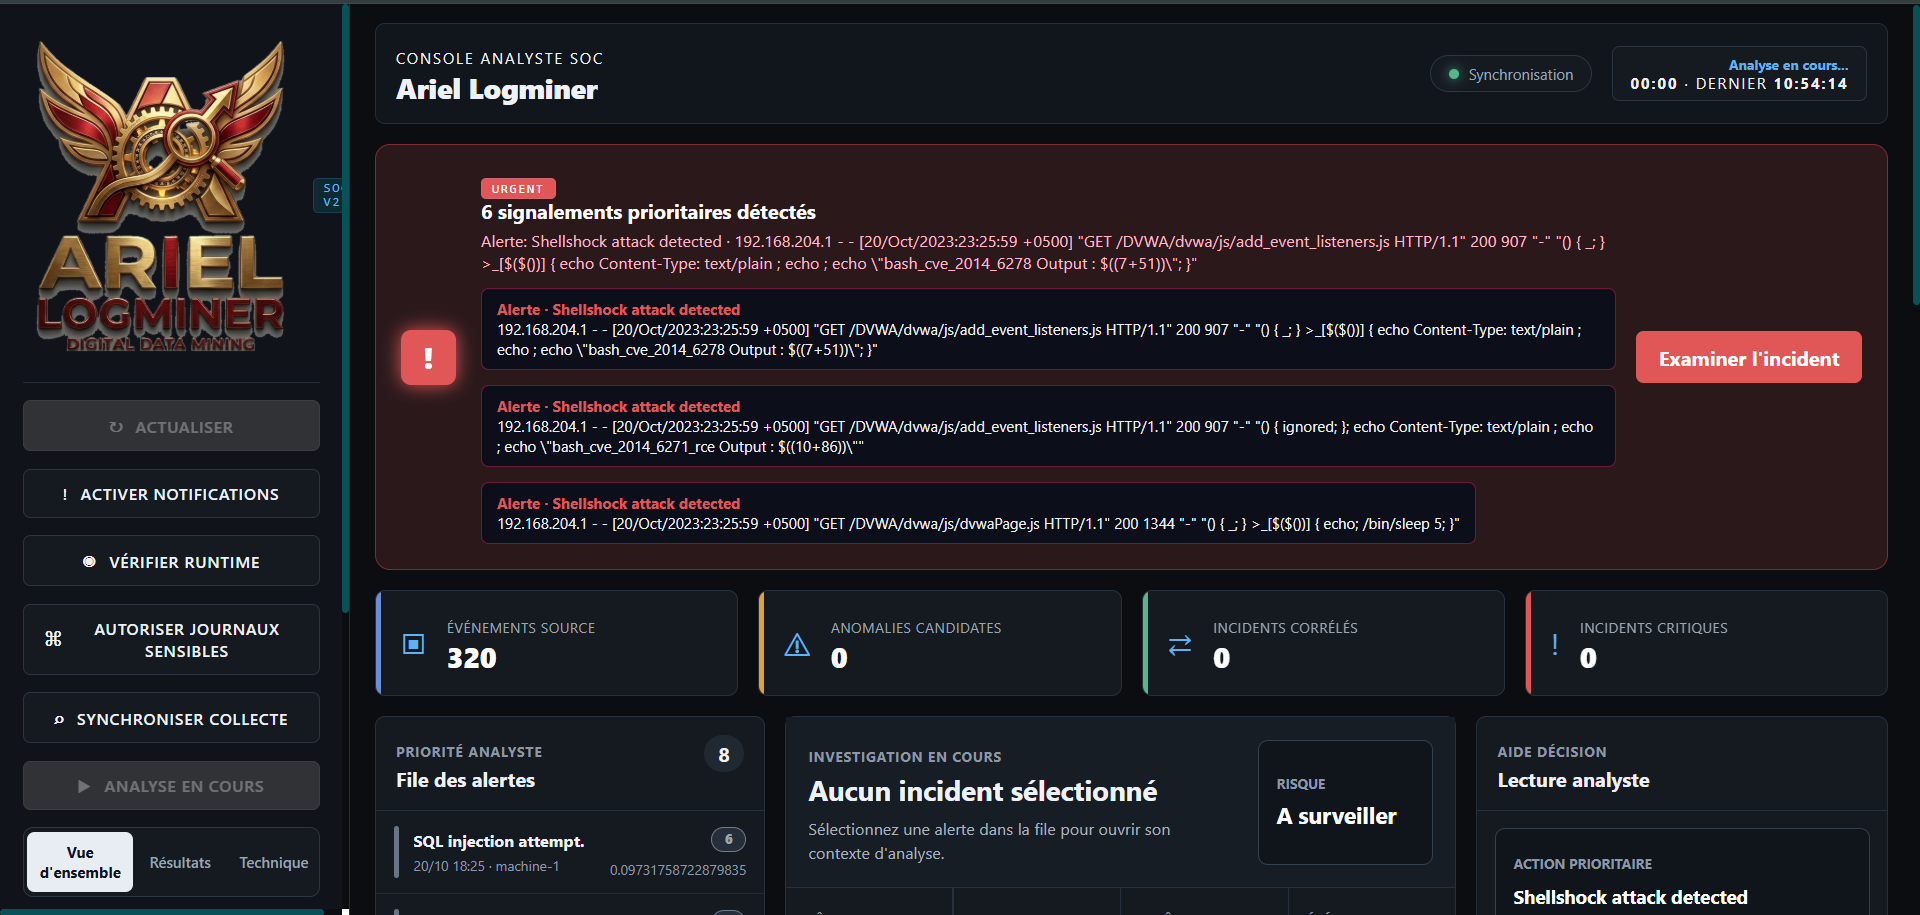
\includegraphics[width=0.94\textwidth]{dashboard_vue_ensemble.png}
    \caption{Vue d'ensemble du tableau de bord. L'interface rassemble les volumes, états et alertes et relie une exécution à ses résultats. Sa validation est fonctionnelle et distincte de l'évaluation prédictive. Source : prototype local Ariel Logminer.}
    \label{fig:dashboard-vue-ensemble}
\end{figure}


\section{Validation fonctionnelle}

Les tests automatisés vérifient notamment les contrats, les transitions du protocole, le routage, les chemins de fallback et le replay idempotent. Le module du noyau multi-agent comprend onze scénarios, dont l'enchaînement de handlers, la persistance et le rechargement d'un objectif, la délégation effective par Contract Net, l'arrêt sur épuisement du budget et la reprise après augmentation explicite de ce budget. Ils sont complétés par les campagnes expérimentales, qui produisent des artefacts CSV et JSON destinés à l'analyse.

Il faut toutefois distinguer deux types de conclusion. Un test fonctionnel réussi montre qu'un chemin du code produit le comportement attendu dans les conditions prévues. Il ne démontre pas qu'une méthode est statistiquement meilleure qu'une autre. Cette seconde question nécessite un protocole expérimental et des métriques adaptées.

Les manifestes conservent la provenance des jeux de données ainsi que l'unité d'analyse retenue pour chaque campagne. Dans le cas du routeur open-set, les contrôles évitent également d'interpréter le score heuristique comme une probabilité calibrée. De la même manière, les expériences distribuées distinguent le fonctionnement du transport Redis de l'autonomie décisionnelle des agents.


\section{Lien entre code et preuves}

Chaque campagne possède un identifiant d'exécution et enregistre ses paramètres avec les résultats qu'elle produit. Cette liaison permet de retrouver l'origine d'une valeur sans dépendre d'une transcription manuelle.

Les figures présentées dans le chapitre suivant sont générées directement à partir de ces artefacts CSV ou JSON. Un script commun centralise le style des graphiques, les unités et les sources utilisées. Cette organisation réduit le risque qu'un tableau, une figure et le texte du mémoire rapportent des valeurs différentes pour une même expérience.


% Chapitre 4
\chapter{Résultats et évaluation}

\label{chap:resultats}

\section{Cadre de lecture}

Ce chapitre présente les campagnes en maintenant séparées les expériences qui ne répondent pas à la même question. Chaque résultat reste rattaché à son jeu de données, à son unité d’analyse, à sa partition et au modèle utilisé. Les campagnes sont désignées par une étiquette lisible (par exemple « campagne HDFS, test complet ») ; chaque étiquette renvoie à une ligne de la matrice de traçabilité (tableau~\ref{tab:preuves-experimentales}), qui donne l'identifiant de la campagne et le chemin de ses artefacts. Dans le texte, les scores sont arrondis à quatre décimales ; la matrice et les fichiers CSV et JSON conservent une précision supérieure.

Quatre ensembles d’expériences structurent la lecture. Les campagnes CICIDS2017, HDFS, BGL et CSE-CIC-IDS2018 portent sur la qualité prédictive et sur la manière dont le protocole modifie son interprétation. Le routeur, la spécialisation des modèles et la couverture multiformat concernent le fonctionnement de la chaîne plutôt que la seule prédiction. Un troisième ensemble étudie le coût des architectures, le Contract Net et la mémoire. La validation sur deux machines virtuelles et la corrélation complètent l’évaluation.

\begin{table}[H]
\centering
\caption{Synthèse des protocoles expérimentaux.}
\label{tab:protocoles-experimentaux}
\small
\begin{tabularx}{\textwidth}{p{0.20\textwidth} p{0.22\textwidth} X}
\toprule
\textbf{Axe} & \textbf{Unité} & \textbf{Question contrôlée} \\
\midrule
CICIDS2017 & flux réseau & Sensibilité au protocole ; cinq candidats sous holdout par scénario. \\
HDFS & bloc & Détection alignée sur le label, parseur ajusté sur l'entraînement seulement. \\
BGL & événement/template & Apport d’Histogram au-delà d’une règle de nouveauté. \\
CSE-CIC-IDS2018 & flux réseau & Audit du transfert entre deux journées et des raccourcis de caractéristiques. \\
Routeur & fichier & Reconnaissance des sources connues et rejet de 20 fichiers inconnus relevant de 16 schémas. \\
Spécialisation & flux, ligne & Modèle propre à chaque famille contre modèle commun. \\
Multiformat & unité native & Lecture, parsing et normalisation des sources testées. \\
Multi-agent & tâche & Coût A--D, panne, mémoire, Contract Net face à une table statique et au moindre chargé. \\
Multi-VM & tâche & Répartition Debian--Ubuntu, reprise et idempotence. \\
Corrélation & paire d'anomalies & Regroupement en incidents sur corpus synthétiques, face aux baselines « hôte et fenêtre » et « fenêtre seule ». \\
\bottomrule
\end{tabularx}
\end{table}

\section{CICIDS2017 : influence du protocole}
\label{sec:cicids-resultats}

\subsection{Question et données}

Les fichiers utilisés sont les CSV d'origine diffusés par le CIC (\texttt{MachineLearningCVE}), sans les corrections proposées par Engelen et al.~\cite{engelen2021troubleshooting} ; les défauts d'étiquetage qu'ils recensent y restent présents. Le holdout par scénario a été répété sur leur version régénérée et réétiquetée (section~\ref{sec:cicids-wtmc}). Trois partitions sont comparées. La séparation aléatoire stratifiée mélange les scénarios : ses lignes sont tirées parmi les premières lignes de chaque fichier, puis rééchantillonnées. Le holdout par scénario réserve au test un fichier d'attaque entier. Le protocole temporel entraîne sur les données du lundi au jeudi et teste le vendredi. Les attaques du vendredi (DDoS, PortScan, Bot) n'apparaissent pas du lundi au jeudi : ce protocole est donc aussi un holdout par catégorie d'attaque, et non une simple séparation chronologique à catégories constantes. La séparation aléatoire et le protocole temporel rassemblent cinq graines ; le holdout par scénario, vingt-cinq évaluations par modèle.

\begin{figure}[H]
  \centering
  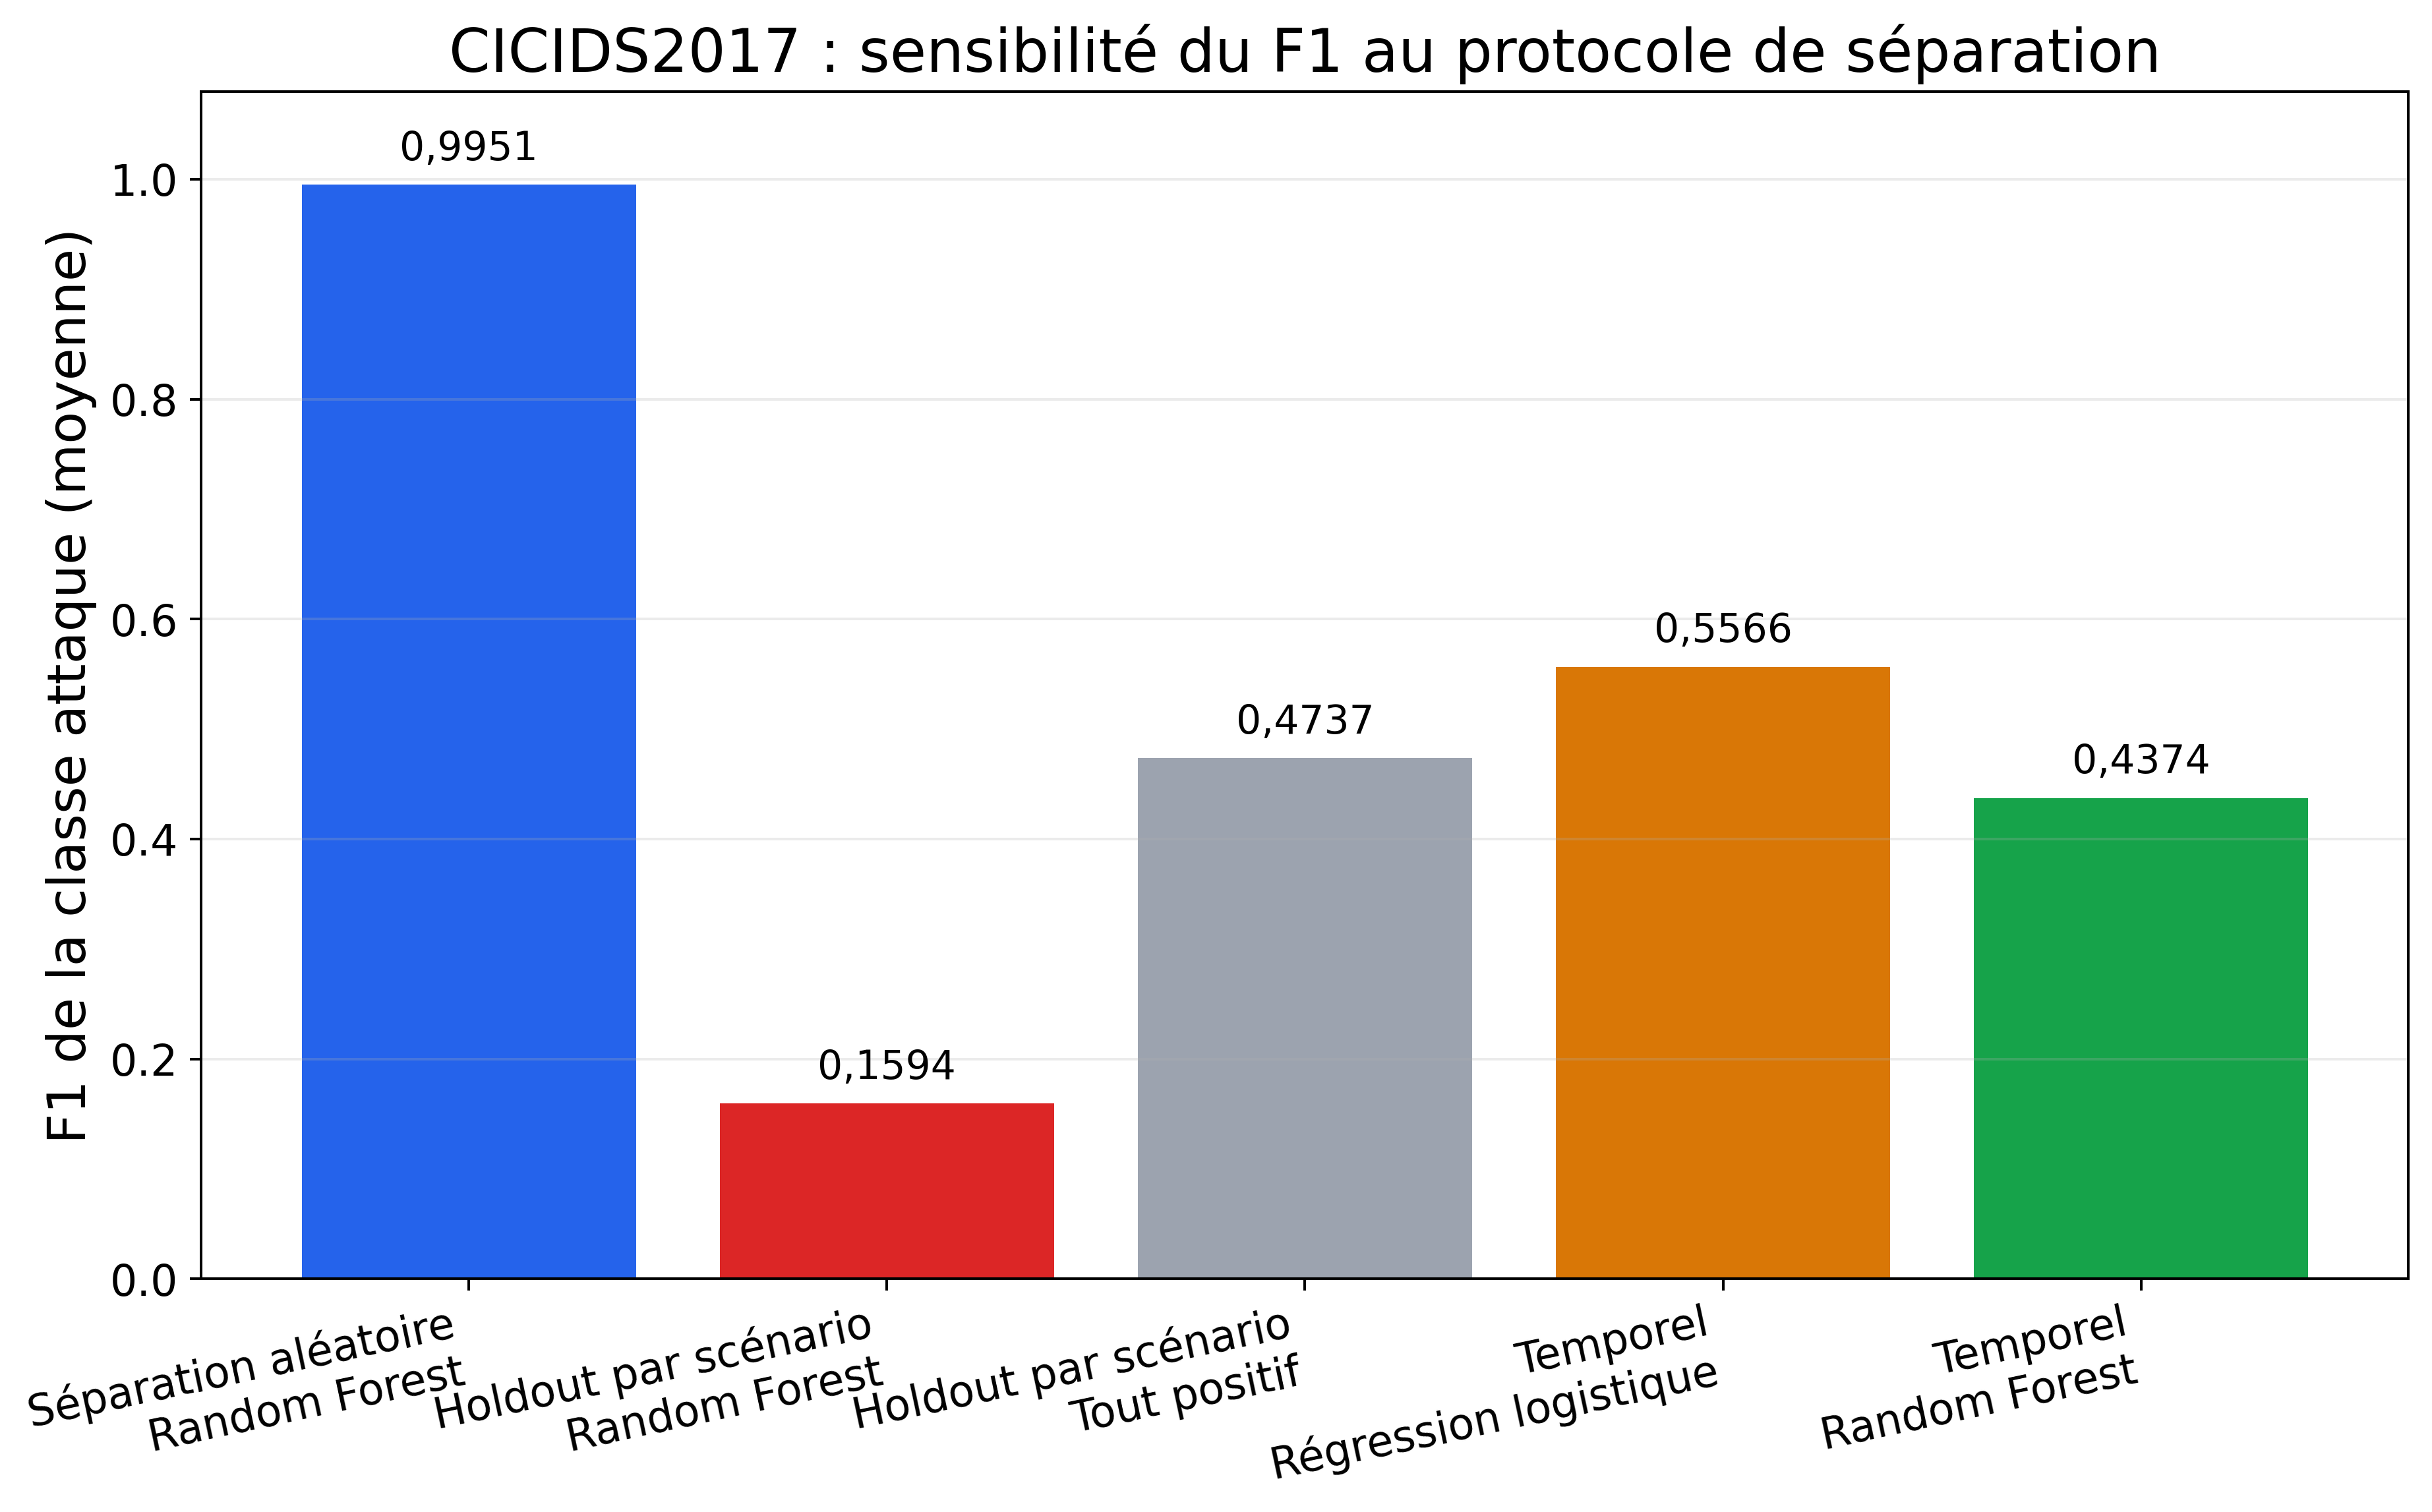
\includegraphics[width=0.98\textwidth]{fig_cicids_protocol_comparison.png}
  \caption[Comparaison des protocoles CICIDS2017.]{F1 de la classe attaque sous les trois protocoles CICIDS2017 ; pour le holdout par scénario, la prédiction systématiquement positive est évaluée sur les mêmes tests. Sources : comparaison des protocoles CICIDS2017 et réexécution du holdout par scénario (tableau~\ref{tab:preuves-experimentales}).}
  \label{fig:cicids-protocoles}
\end{figure}

La lecture change nettement avec la partition. Lorsque l’entraînement et le test partagent la structure des scénarios, le Random Forest sépare presque parfaitement les observations ($0{,}9951$). Ce score chute dès qu’un scénario entier est tenu hors de l’entraînement. Sous la séparation temporelle, qui tient elle aussi hors de l'entraînement les catégories du vendredi, la régression logistique ($0{,}5566$) dépasse le Random Forest ($0{,}4374$). Ce protocole n'est donc pas intermédiaire entre les deux autres : il tient lui aussi des catégories hors de l'entraînement, sur un test de composition différente. Ces scores sont des propriétés des protocoles testés, non une estimation de la performance attendue sur un réseau jamais observé.

\subsection{Cinq candidats sous holdout par scénario}

Cinq classificateurs (\texttt{LogisticRegression}, \texttt{SGDLogistic}, \texttt{HistGradientBoosting}, \texttt{RandomForest} et \texttt{ExtraTrees}) sont comparés avec les mêmes variables, les mêmes échantillons et les mêmes graines. Chaque scénario d'attaque (DDoS, PortScan, Bot, Infiltration, WebAttacks) est tour à tour tenu à l'écart, pour chacune des graines 42 à 46. L'entraînement tire au hasard $8\,000$ lignes par classe dans l'ensemble des sept autres fichiers, en respectant leurs proportions ; le test tire au plus $4\,000$ lignes par classe dans le fichier tenu à l'écart. Ces plafonds sont des paramètres de configuration, non le résultat d'un calcul de puissance. Les tests comptent ainsi $8\,000$ lignes pour DDoS et PortScan, $6\,180$ pour WebAttacks, $5\,966$ pour Bot et $4\,036$ pour Infiltration, dont 36 attaques seulement, qui pèsent pourtant autant que les autres scénarios dans la moyenne. Le F1 est calculé à la règle de décision par défaut de chaque modèle, sans seuil calibré.

Une première exécution de ce protocole tirait les lignes dans l'ordre des fichiers : les plafonds étaient atteints dès le premier fichier lu, si bien que l'entraînement ne contenait qu'un scénario d'attaque, DDoS ou PortScan. Ses résultats ne sont pas retenus. Le protocole présenté ici, qui ne modifie que le tirage des lignes, a été versionné avant son exécution ; la règle de décision fixée à cette occasion demande qu'un modèle dépasse la prédiction systématiquement positive de plus de $0{,}01$ en F1 moyen et sur au moins quatre des cinq scénarios.

\begin{table}[H]
\centering
\caption[Cinq candidats CICIDS2017 sous holdout par scénario.]{Cinq candidats CICIDS2017 sous holdout par scénario : F1 moyen par scénario tenu à l'écart (cinq graines), F1 moyen sur les 25 évaluations et F1 micro (matrices de confusion cumulées). Source : réexécution du holdout par scénario (tableau~\ref{tab:preuves-experimentales}).}
\label{tab:cicids-candidats}
\footnotesize
\setlength{\tabcolsep}{4pt}
\begin{tabular}{lrrrrrrr}
\toprule
\textbf{Modèle} & \textbf{DDoS} & \textbf{PortScan} & \textbf{Bot} & \textbf{Infiltr.} & \textbf{WebAtt.} & \textbf{F1 moyen} & \textbf{F1 micro} \\
\midrule
Tout positif & 0,6667 & 0,6667 & 0,4957 & 0,0177 & 0,5215 & 0,4737 & 0,5492 \\
SGDLogistic & 0,7618 & 0,1030 & 0,3707 & 0,0073 & 0,1916 & 0,2869 & 0,4251 \\
LogisticRegression & 0,7410 & 0,0993 & 0,3828 & 0,0178 & 0,0170 & 0,2516 & 0,3840 \\
HistGradientBoosting & 0,7746 & 0,0099 & 0,0000 & 0,0004 & 0,2790 & 0,2128 & 0,3805 \\
RandomForest & 0,7745 & 0,0027 & 0,0000 & 0,0047 & 0,0151 & 0,1594 & 0,3433 \\
ExtraTrees & 0,7378 & 0,0028 & 0,0000 & 0,0000 & 0,0427 & 0,1567 & 0,3085 \\
\bottomrule
\end{tabular}
\end{table}

Aucun des cinq modèles ne satisfait la règle de décision : tous restent sous la prédiction systématiquement positive en F1 moyen comme en F1 micro. Les modèles ne la dépassent nettement que sur DDoS, et la régression logistique l'égale sur Infiltration, dont le score est dominé par 36 attaques. Sur PortScan, Bot et WebAttacks, une attaque absente de l'entraînement est le plus souvent classée bénigne. Le classement entre candidats est secondaire : SGDLogistic n'est le meilleur qu'au sens d'une désignation faite après coup parmi cinq modèles, et il dépend du seuil par défaut, comme le montre HistGradientBoosting, dont la PR-AUC moyenne est la plus élevée ($0{,}6577$) alors que son F1 reste faible.

\paragraph{Version corrigée de CICIDS2017.}\label{sec:cicids-wtmc} Le même holdout par scénario a été répété, sous un protocole versionné avant son exécution, sur la version régénérée et réétiquetée de CICIDS2017 publiée par Engelen, Rimmer et Joosen (5 fichiers journaliers, $2\,100\,814$ flux). Les cinq modèles, leurs hyperparamètres, les graines, les plafonds et la règle de décision sont inchangés ; les identifiants (adresses, port source, protocole, horodatage) sont retirés des variables. Une première variante exclut les flux étiquetés « tentés » (\textit{Attempted}), attaques sans effet. Une seconde, décidée après lecture de ce résultat, suit la recommandation des auteurs et les compte comme bénins. La décision est identique dans les deux variantes : aucun modèle ne dépasse la prédiction systématiquement positive. Avec exclusion, leur F1 moyen vaut $0{,}20$ à $0{,}23$ contre $0{,}34$ ; avec reclassement bénin, il vaut $0{,}20$ à $0{,}22$ contre $0{,}34$, et au plus deux scénarios sur cinq sont gagnés. Sur ces données, DDoS se transfère presque parfaitement (F1 de $0{,}99$ dans la première variante), tandis que PortScan, Bot et les attaques web restent au niveau du hasard ou en dessous (MCC d'au plus $0{,}03$ dans cette variante). La réfutation sous le critère préenregistré ne tient donc ni aux défauts du jeu d'origine ni au traitement des flux tentés dans ce dispositif.

\subsection{Contrôle non supervisé sous protocole temporel}

Les campagnes précédentes relèvent de la classification supervisée. Pour mesurer le comportement d'un détecteur n'ayant vu aucune attaque à l'apprentissage, un Isolation Forest \cite{liu2008isolation} est ajusté sur $10\,000$ flux bénins de lundi à jeudi, puis évalué sur les mêmes tests du vendredi que la régression logistique et le Random Forest du protocole temporel, pour les graines 42 à 46. Deux seuils sont fixés sur une validation disjointe de l'ajustement : le quantile 99~\% des scores bénins, qui n'utilise que des données normales, et le seuil maximisant le F1 de validation, qui utilise aussi les attaques de cette partition.

\begin{table}[H]
\centering
\caption[Contrôle Isolation Forest sur CICIDS2017.]{Isolation Forest et modèles supervisés sur le même test temporel CICIDS2017, cinq graines. Sources : contrôle Isolation Forest et campagne CICIDS2017 en séparation temporelle.}
\label{tab:cicids-iforest}
\small
\begin{tabular}{llrrrr}
\toprule
\textbf{Modèle} & \textbf{Seuil} & \textbf{F1 moyen} & \textbf{Rappel} & \textbf{FPR} & \textbf{PR-AUC} \\
\midrule
Isolation Forest & quantile bénin 99~\% & 0,1157 & 0,0635 & 0,0334 & 0,5718 \\
Isolation Forest & max. F1 validation & 0,5214 & 0,5195 & 0,3123 & 0,5718 \\
LogisticRegression & supervisé & 0,5566 & 0,4010 & 0,0394 & 0,8714 \\
RandomForest & supervisé & 0,4374 & 0,2806 & 0,0024 & 0,8308 \\
\bottomrule
\end{tabular}
\end{table}

Le classement produit par Isolation Forest reste peu discriminant, avec une ROC-AUC moyenne de $0{,}6390$. Le seuil appris sur le trafic bénin seul ne détecte que $6{,}35\,\%$ des attaques ; le seuil optimisé sur la validation relève le rappel au prix d'un FPR moyen de $0{,}3123$ et d'une forte dispersion du F1 entre graines ($0{,}1708$). Sur ce test équilibré, une prédiction systématiquement positive obtiendrait un F1 de $0{,}6667$. Ce contrôle ne soutient donc pas le remplacement des classificateurs supervisés par ce détecteur générique ; l'évaluation des flux réseau porte principalement sur une classification supervisée.

\section{HDFS : décision au niveau bloc}

\subsection{Protocole sans contamination du parseur}

Le fichier HDFS contient $11\,175\,629$ lignes et $575\,061$ blocs annotés. Les blocs sont ordonnés par première apparition, puis répartis selon des proportions 60/20/20 : $345\,036$ blocs d'entraînement, $115\,012$ de validation et $115\,013$ de test, dont respectivement $11\,158$, $4\,001$ et $1\,679$ positifs (campagne HDFS, test complet). La prévalence vaut donc $3{,}23\,\%$, $3{,}48\,\%$ et $1{,}46\,\%$ : la baisse au test tient à l'ordre chronologique de la partition et non à un échantillonnage. Elle a un effet mécanique : à rappel et taux de faux positifs égaux, une prévalence plus faible abaisse la précision, et le seuil choisi en validation n'est pas optimal pour le test. Pour chacune des graines 42 à 46, $6\,000$ blocs d'entraînement (194 positifs, $1{,}7\,\%$ de l'entraînement) sont tirés de façon stratifiée pour ajuster le parseur ; cette taille est un paramètre du protocole, et la sensibilité du résultat à cette taille n'a pas été évaluée. La validation et le test sont utilisés en entier.

Pour chaque graine, Drain3 est ajusté uniquement sur les événements des blocs d'entraînement tirés avec \texttt{sim\_th=0.4}, profondeur 4 et 100 enfants au maximum. La validation et le test utilisent \texttt{match\_only}. L'empreinte de l’état et le nombre de clusters (24 à 36 selon la graine) sont identiques avant et après inférence, ce qui confirme l’absence de mise à jour du parseur ; deux exécutions indépendantes produisent des états de même empreinte et des métriques identiques. Les scores de rareté événementiels d'Histogram, qui suit le principe de HBOS (sous-section~\ref{subsec:histogram}), sont regroupés par bloc ; l’agrégateur et le seuil sont choisis sur validation seulement.

\begin{figure}[H]
  \centering
  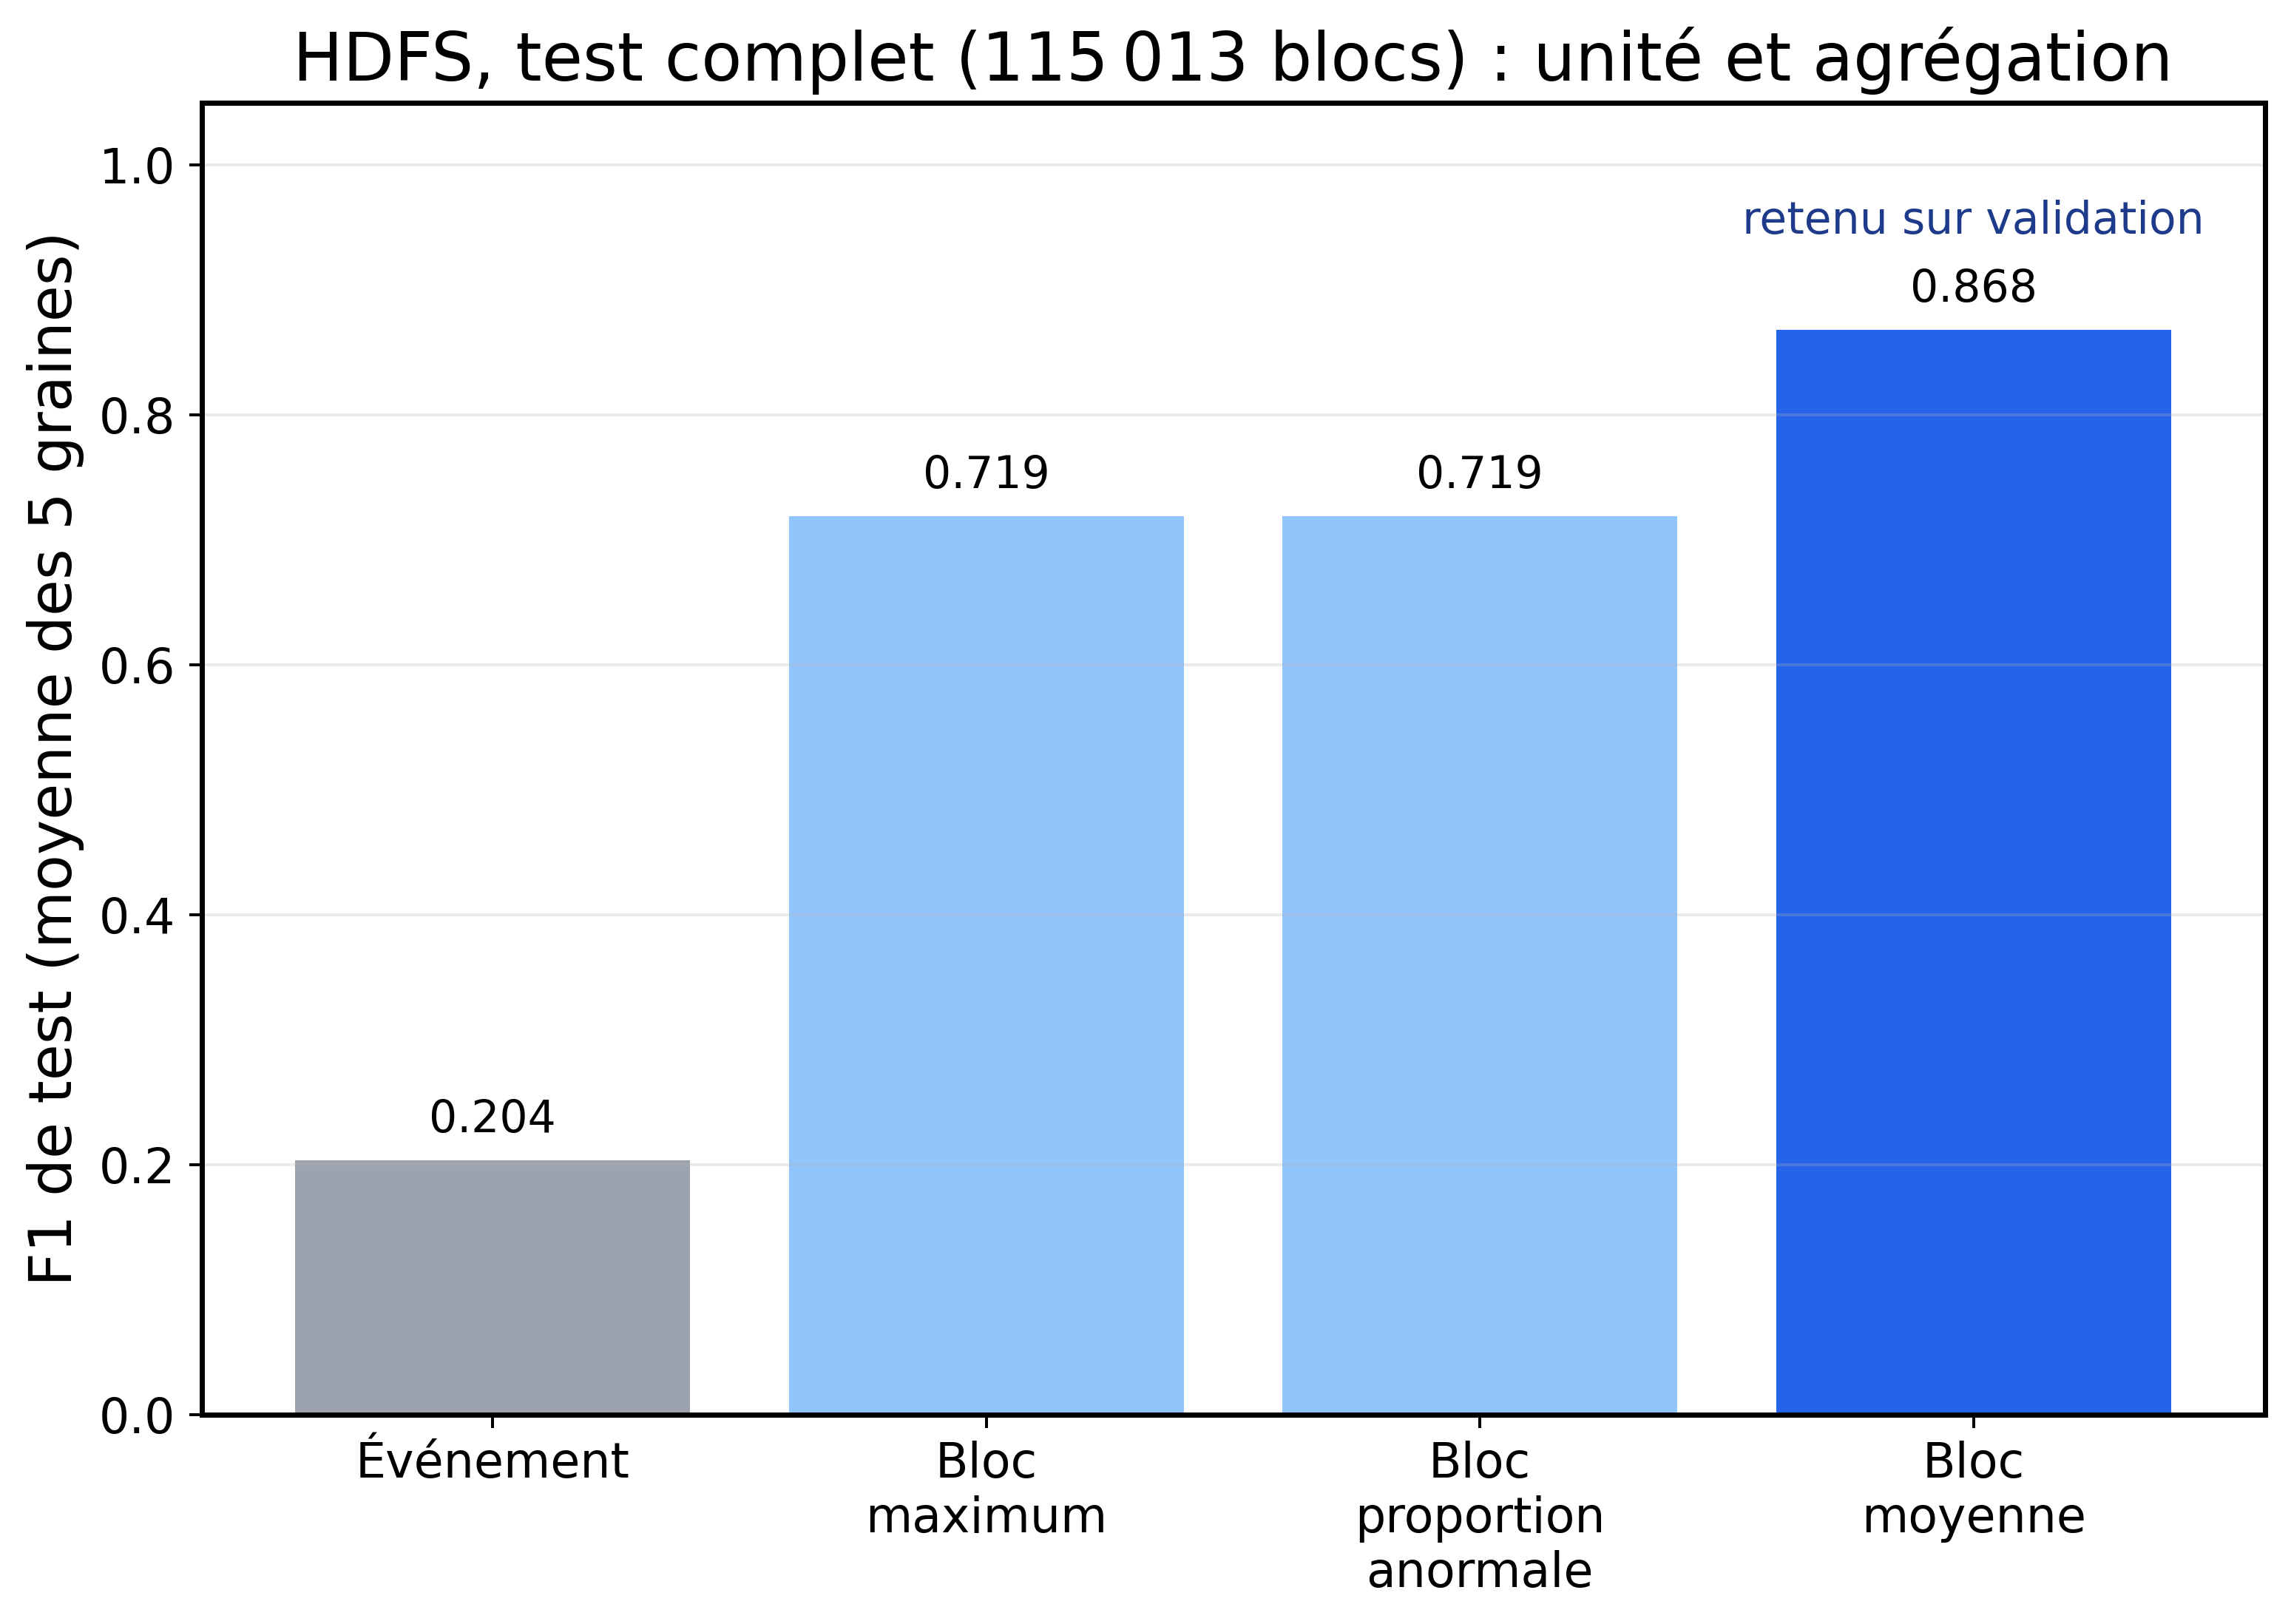
\includegraphics[width=0.96\textwidth]{fig_hdfs_event_vs_block.png}
  \caption[F1 HDFS au niveau événement et au niveau bloc.]{F1 de test HDFS au niveau événement et pour les trois agrégations par bloc, sur les $115\,013$ blocs du test ; la matrice de confusion est identique pour les graines 42 à 46. Source : campagne HDFS, test complet.}
  \label{fig:hdfs-event-bloc}
\end{figure}

La validation retient la moyenne pour les cinq graines, avec un seuil compris entre $1{,}2729$ et $1{,}2748$. Sur les $115\,013$ blocs de test, les cinq graines produisent la même matrice de confusion : $1\,679$ vrais positifs, 509 faux positifs, $112\,825$ vrais négatifs et aucun faux négatif. La précision vaut $0{,}7674$ (intervalle exact à 95~\% : $[0{,}7491\,;\,0{,}7849]$), le rappel $1$ ($[0{,}9978\,;\,1]$), le FPR $0{,}0045$ et le F1 $0{,}8684$, identique pour les cinq graines (intervalle bootstrap à 95~\% : $[0{,}8568\,;\,0{,}8795]$). La PR-AUC varie de $0{,}8449$ à $0{,}8502$ selon la graine.

\subsection{Incertitude}

Selon la graine, Drain3 forme de 24 à 36 clusters, mais la matrice de confusion reste identique en validation comme au test. Les cinq graines ne constituent donc qu'une seule observation du test, non cinq observations indépendantes. L'incertitude rapportée porte sur les blocs de test : intervalles exacts de Clopper-Pearson pour la précision, le rappel et le FPR, et bootstrap multinomial de $20\,000$ réplications pour le F1. Sur un échantillon de $2\,000$ blocs du test, dont 29 positifs, également utilisé pour l'exécution distribuée (section~\ref{sec:hdfs-distribue}), le F1 vaut $0{,}8923$ ; mille réplications bootstrap par \texttt{block\_id} donnent une médiane de $0{,}8947$ et un intervalle empirique $[0{,}8000\,;\,0{,}9610]$. Cette valeur se situe hors de l'intervalle du test complet : un échantillon de cette taille surestime la performance.

\begin{figure}[H]
  \centering
  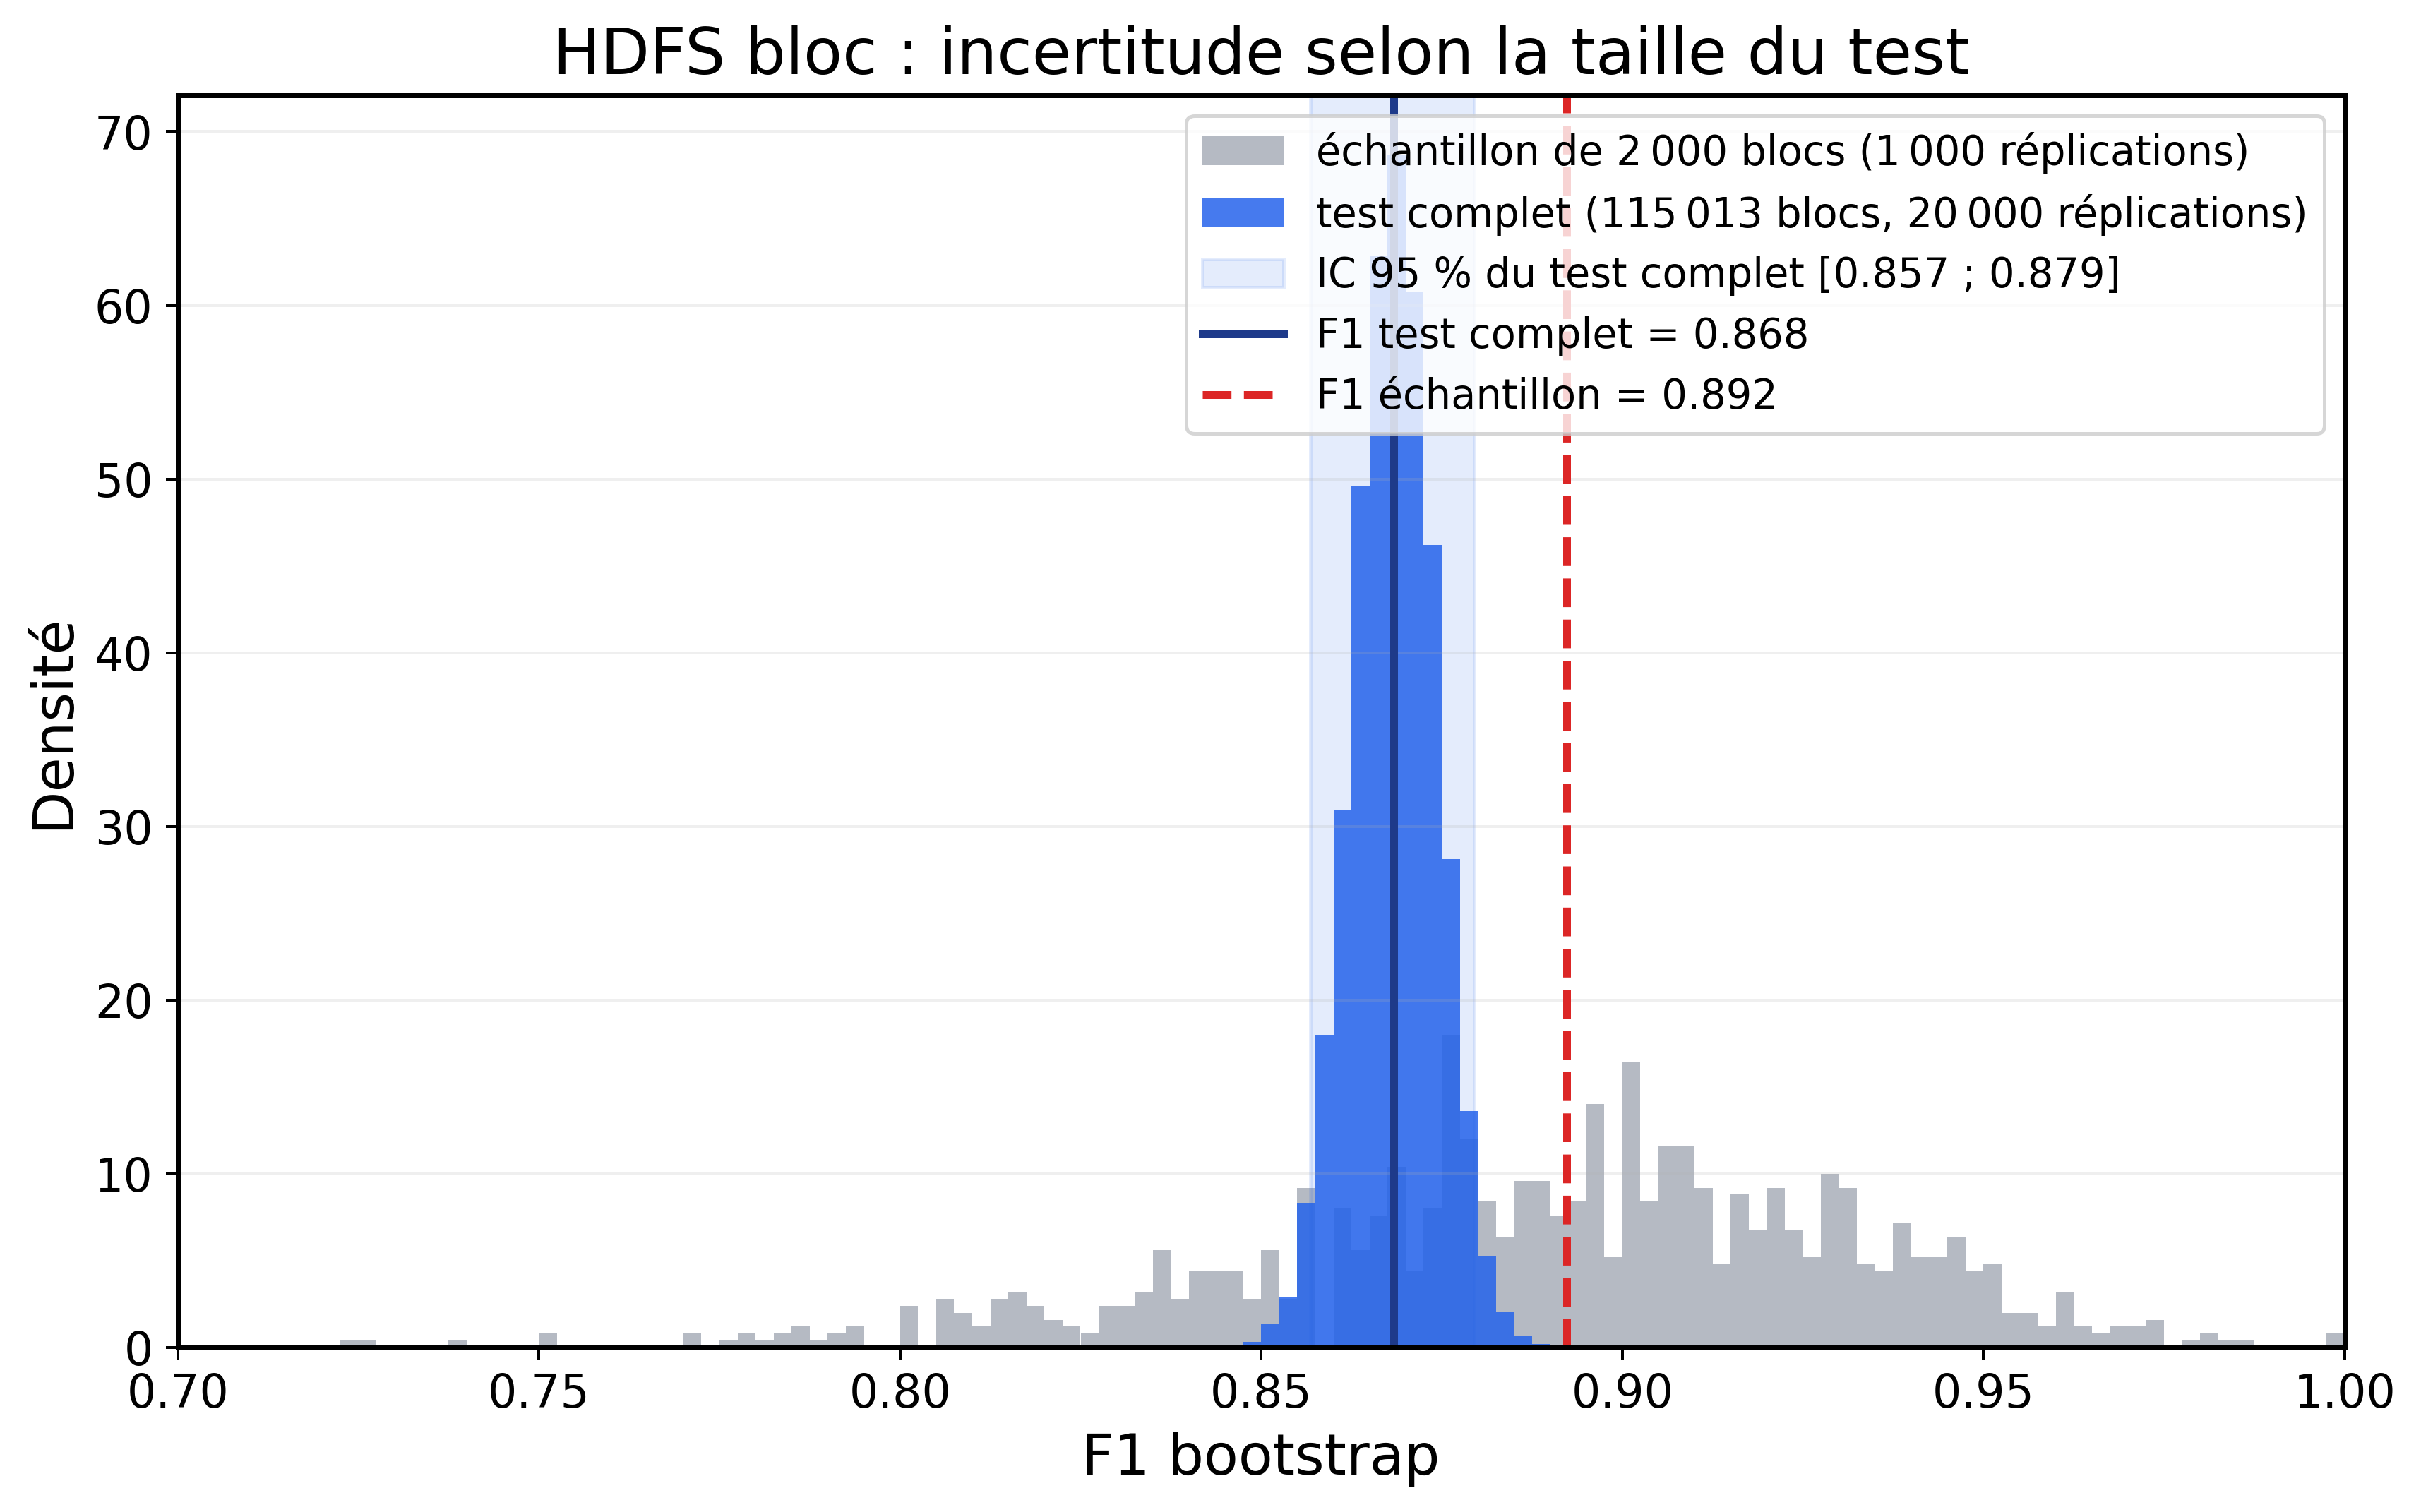
\includegraphics[width=0.96\textwidth]{fig_hdfs_bootstrap_distribution.png}
  \caption[Distribution bootstrap du F1 HDFS : test complet et échantillon de 2\,000 blocs.]{Distribution bootstrap du F1 HDFS sur le test complet ($115\,013$ blocs, $20\,000$ réplications multinomiales) et sur l'échantillon de $2\,000$ blocs ($1\,000$ réplications par \texttt{block\_id}). Sources : campagne HDFS, test complet, et campagne HDFS, échantillon de 2\,000 blocs.}
  \label{fig:hdfs-bootstrap}
\end{figure}

\subsection{Comparaison avec des baselines au niveau bloc}

Le seuil retenu détecte tous les blocs positifs de cette partition, ce qui ne suffit pas à établir un avantage sur une règle simple. Un protocole versionné avant son exécution compare donc Histogram à des règles simples, sur les mêmes partitions et les mêmes graines. La baseline \texttt{template\_only\_mean\_surprisal} calcule, pour chaque bloc, la surprise moyenne de ses templates selon leur fréquence parmi les événements normaux des blocs d'entraînement ; son seuil est choisi sur la validation. C'est la restriction du score d'Histogram au seul template : la comparaison oppose donc Histogram à sa propre version univariée. Histogram agrège les surprises de template, de source et de sévérité.

\begin{table}[H]
\centering
\small
\caption[Baselines au niveau bloc sur le test HDFS complet.]{Baselines au niveau bloc sur le test HDFS complet. Les valeurs sont identiques pour les graines 42 à 46, sauf pour la règle du template inédit (moyenne ; détail au tableau~\ref{tab:hdfs-baselines-seeds}).}
\label{tab:hdfs-block-baselines}
\begin{tabularx}{\textwidth}{Xrrrr}
\toprule
\textbf{Règle} & \textbf{F1} & \textbf{Précision} & \textbf{Rappel} & \textbf{FPR} \\
\midrule
Tout positif & 0,0288 & 0,0146 & 1,0000 & 1,0000 \\
Au moins un template inédit & 0,0191 & 0,9456 & 0,0096 & $<0{,}0001$ \\
Surprise moyenne du template & 0,8724 & 0,7737 & 1,0000 & 0,0043 \\
Histogram (template, source, sévérité) & 0,8684 & 0,7674 & 1,0000 & 0,0045 \\
\bottomrule
\end{tabularx}
\end{table}

La meilleure baseline simple dépasse Histogram de $0{,}0041$ en F1 ; le critère fixé avant exécution exigeait d'Histogram un avantage d'au moins $0{,}01$. Sur le test, les deux règles ont un rappel de 1, mais la baseline produit 491 faux positifs contre 509. Selon la règle de décision, le résultat est dominé par une règle simple.

\section{BGL : templates connus et inconnus}
\label{sec:bgl-resultats}

Le détecteur Histogram est évalué sur $19\,908$ événements, dont $2\,885$ positifs. Son seuil vaut $10{,}82$. Il produit $2\,885$ vrais positifs, 545 faux positifs, $16\,478$ vrais négatifs et aucun faux négatif, soit un F1 de $0{,}9137$. Toutefois, $17\,879$ événements, soit $89{,}81\,\%$, portent un template inconnu.

\begin{figure}[H]
  \centering
  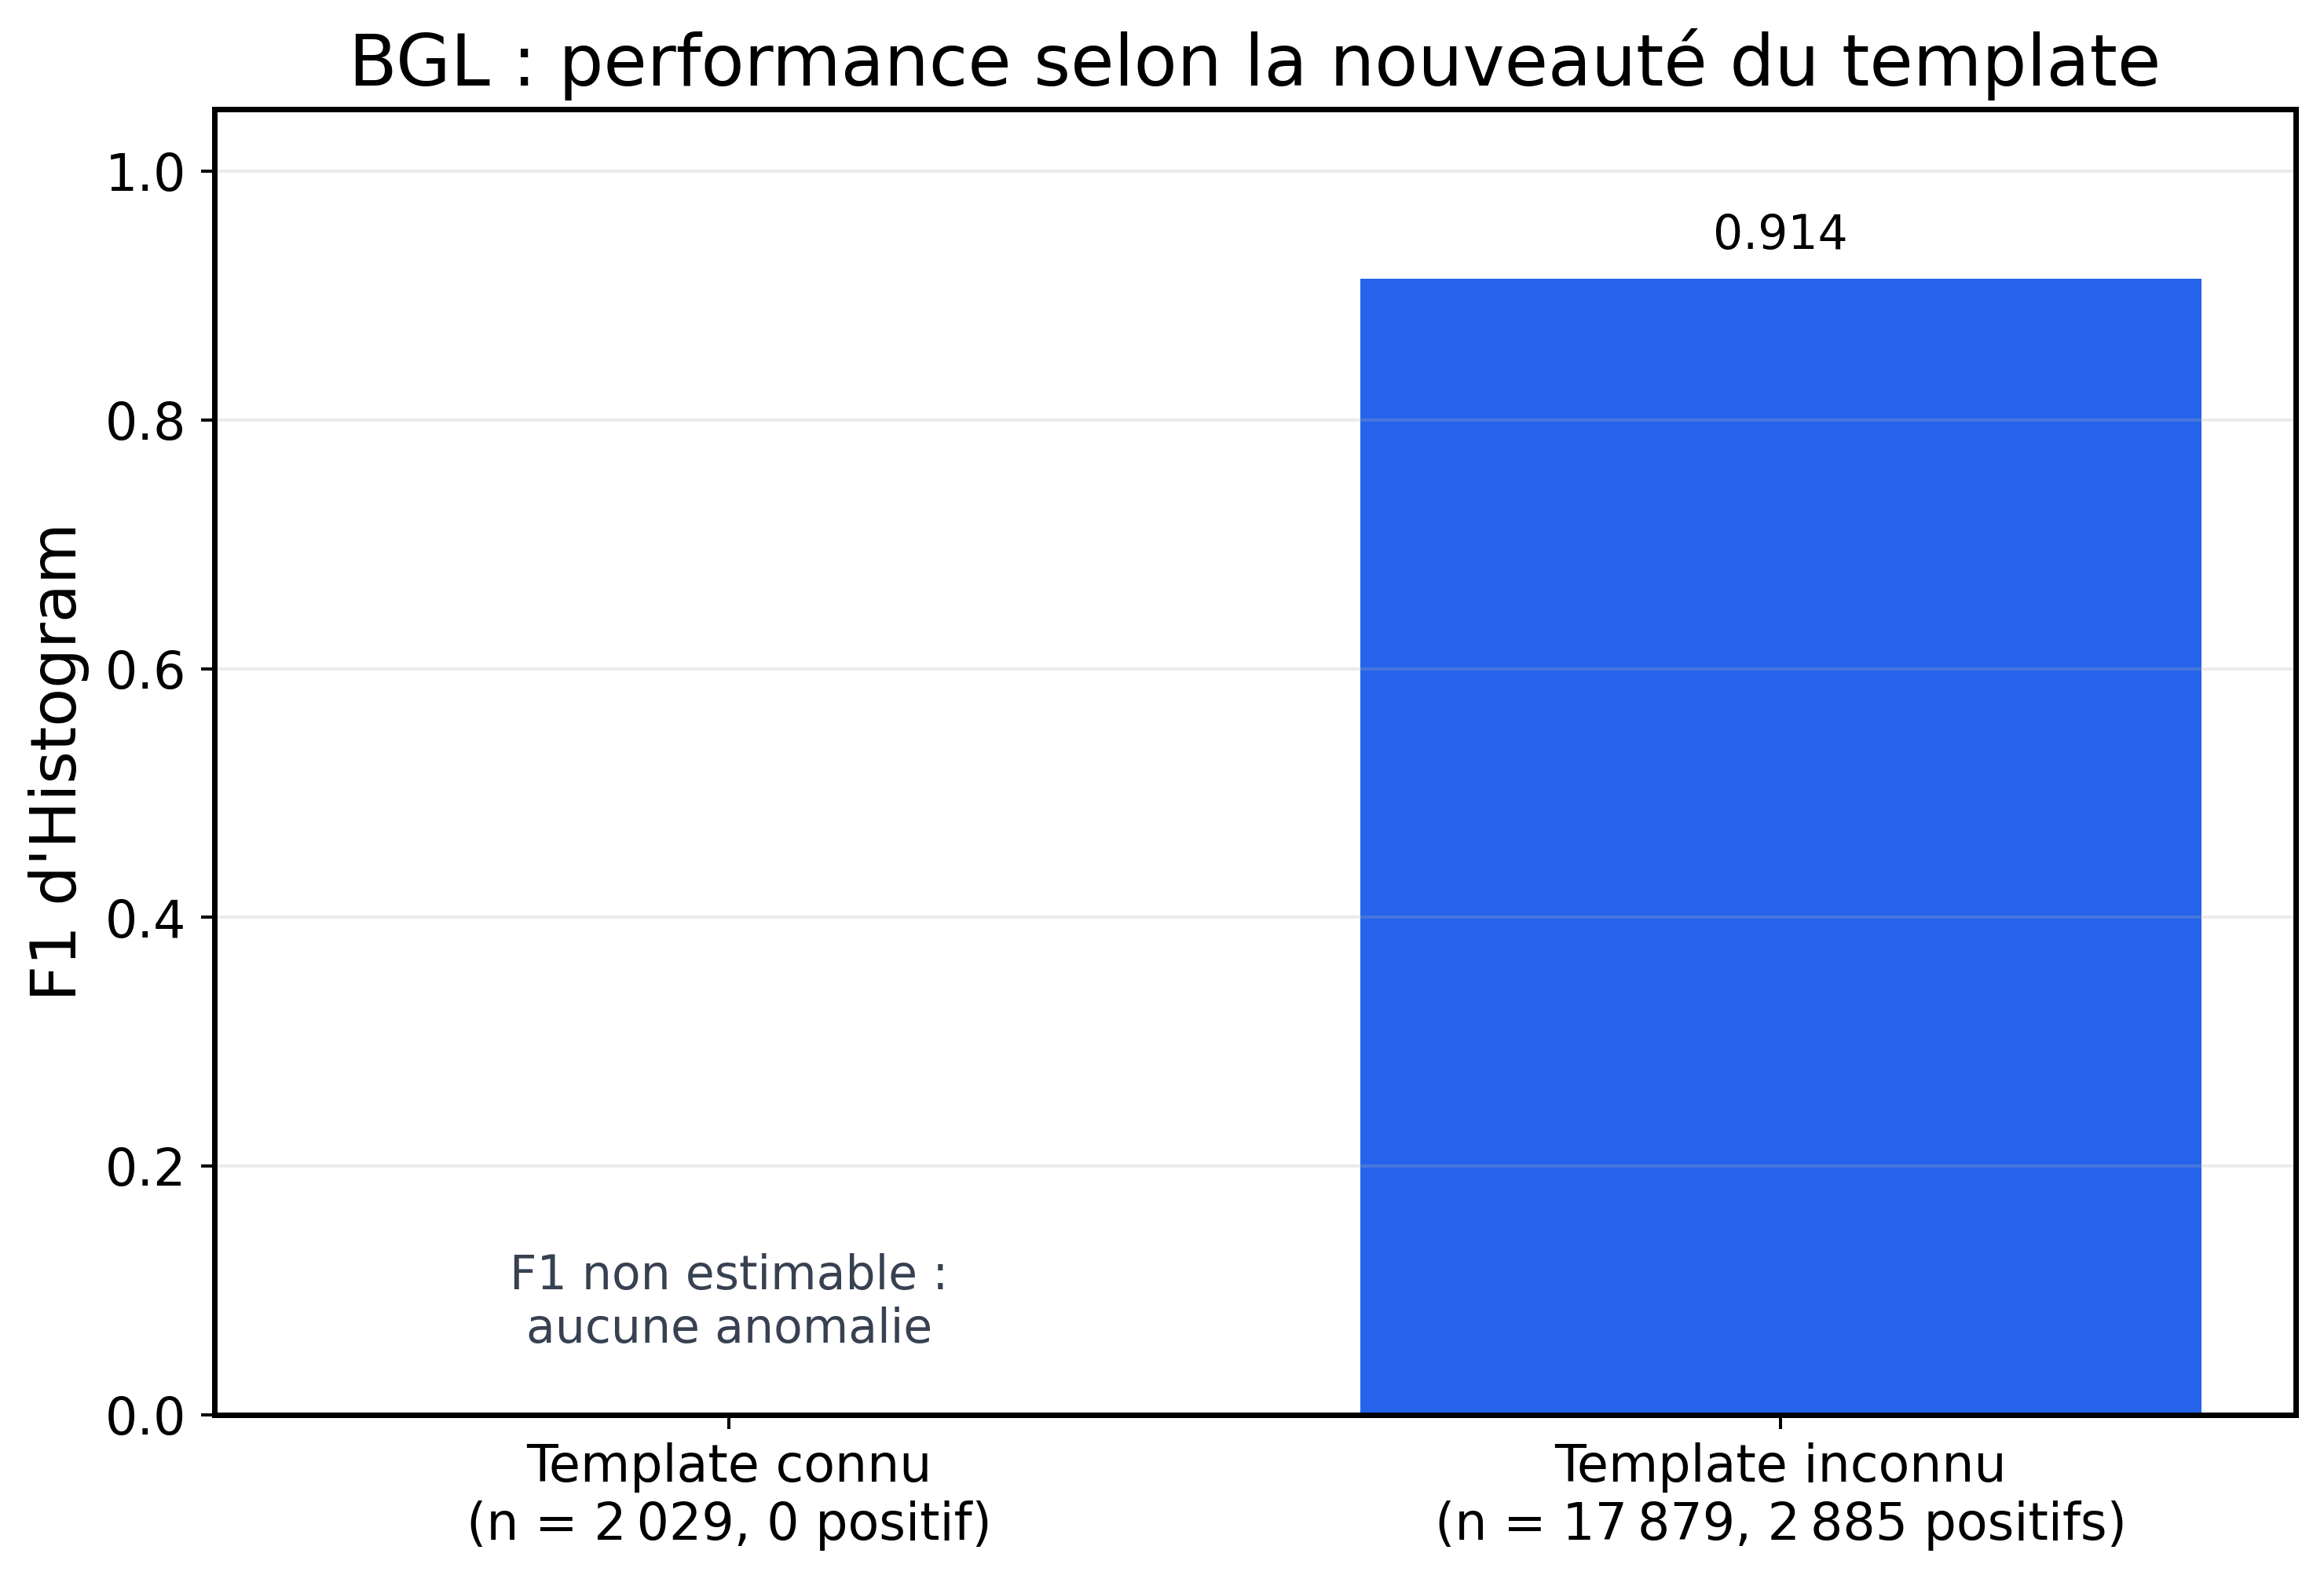
\includegraphics[width=0.96\textwidth]{fig_bgl_known_unknown.png}
  \caption[Résultats BGL selon la connaissance du template.]{F1 d'Histogram sur BGL selon la connaissance du template ; le groupe des templates connus ne contient aucune anomalie. Source : campagne BGL, second protocole, protocole principal.}
  \label{fig:bgl-connu-inconnu}
\end{figure}

La règle \texttt{UnknownTemplateBaseline}, qui déclare anormal tout template inconnu, n'atteint qu'un F1 de $0{,}2779$, avec $14\,994$ faux positifs. Ce protocole est pourtant dégénéré. Les $49\,999$ événements d'entraînement sont tous de sévérité \texttt{INFO} et Drain3 n'y forme que 7 clusters. Le seuil choisi sur validation est égal à $\ln 49\,999$, soit le score maximal possible : un événement n'est déclaré anormal que si son template, sa source et sa sévérité sont tous absents de l'entraînement. Sur ce test, Histogram applique donc exactement la règle « sévérité absente de l'entraînement », qui produit la même matrice de confusion et le même F1. Le F1 de $0{,}9137$ mesure cette règle, et non une capacité de détection apprise. Le contraste entre validation et test le confirme : le F1 de validation n'est que de $0{,}7335$, pour un FPR de $0{,}6128$, contre $0{,}0320$ au test, les deux périodes ayant des compositions très différentes.

\begin{figure}[H]
  \centering
  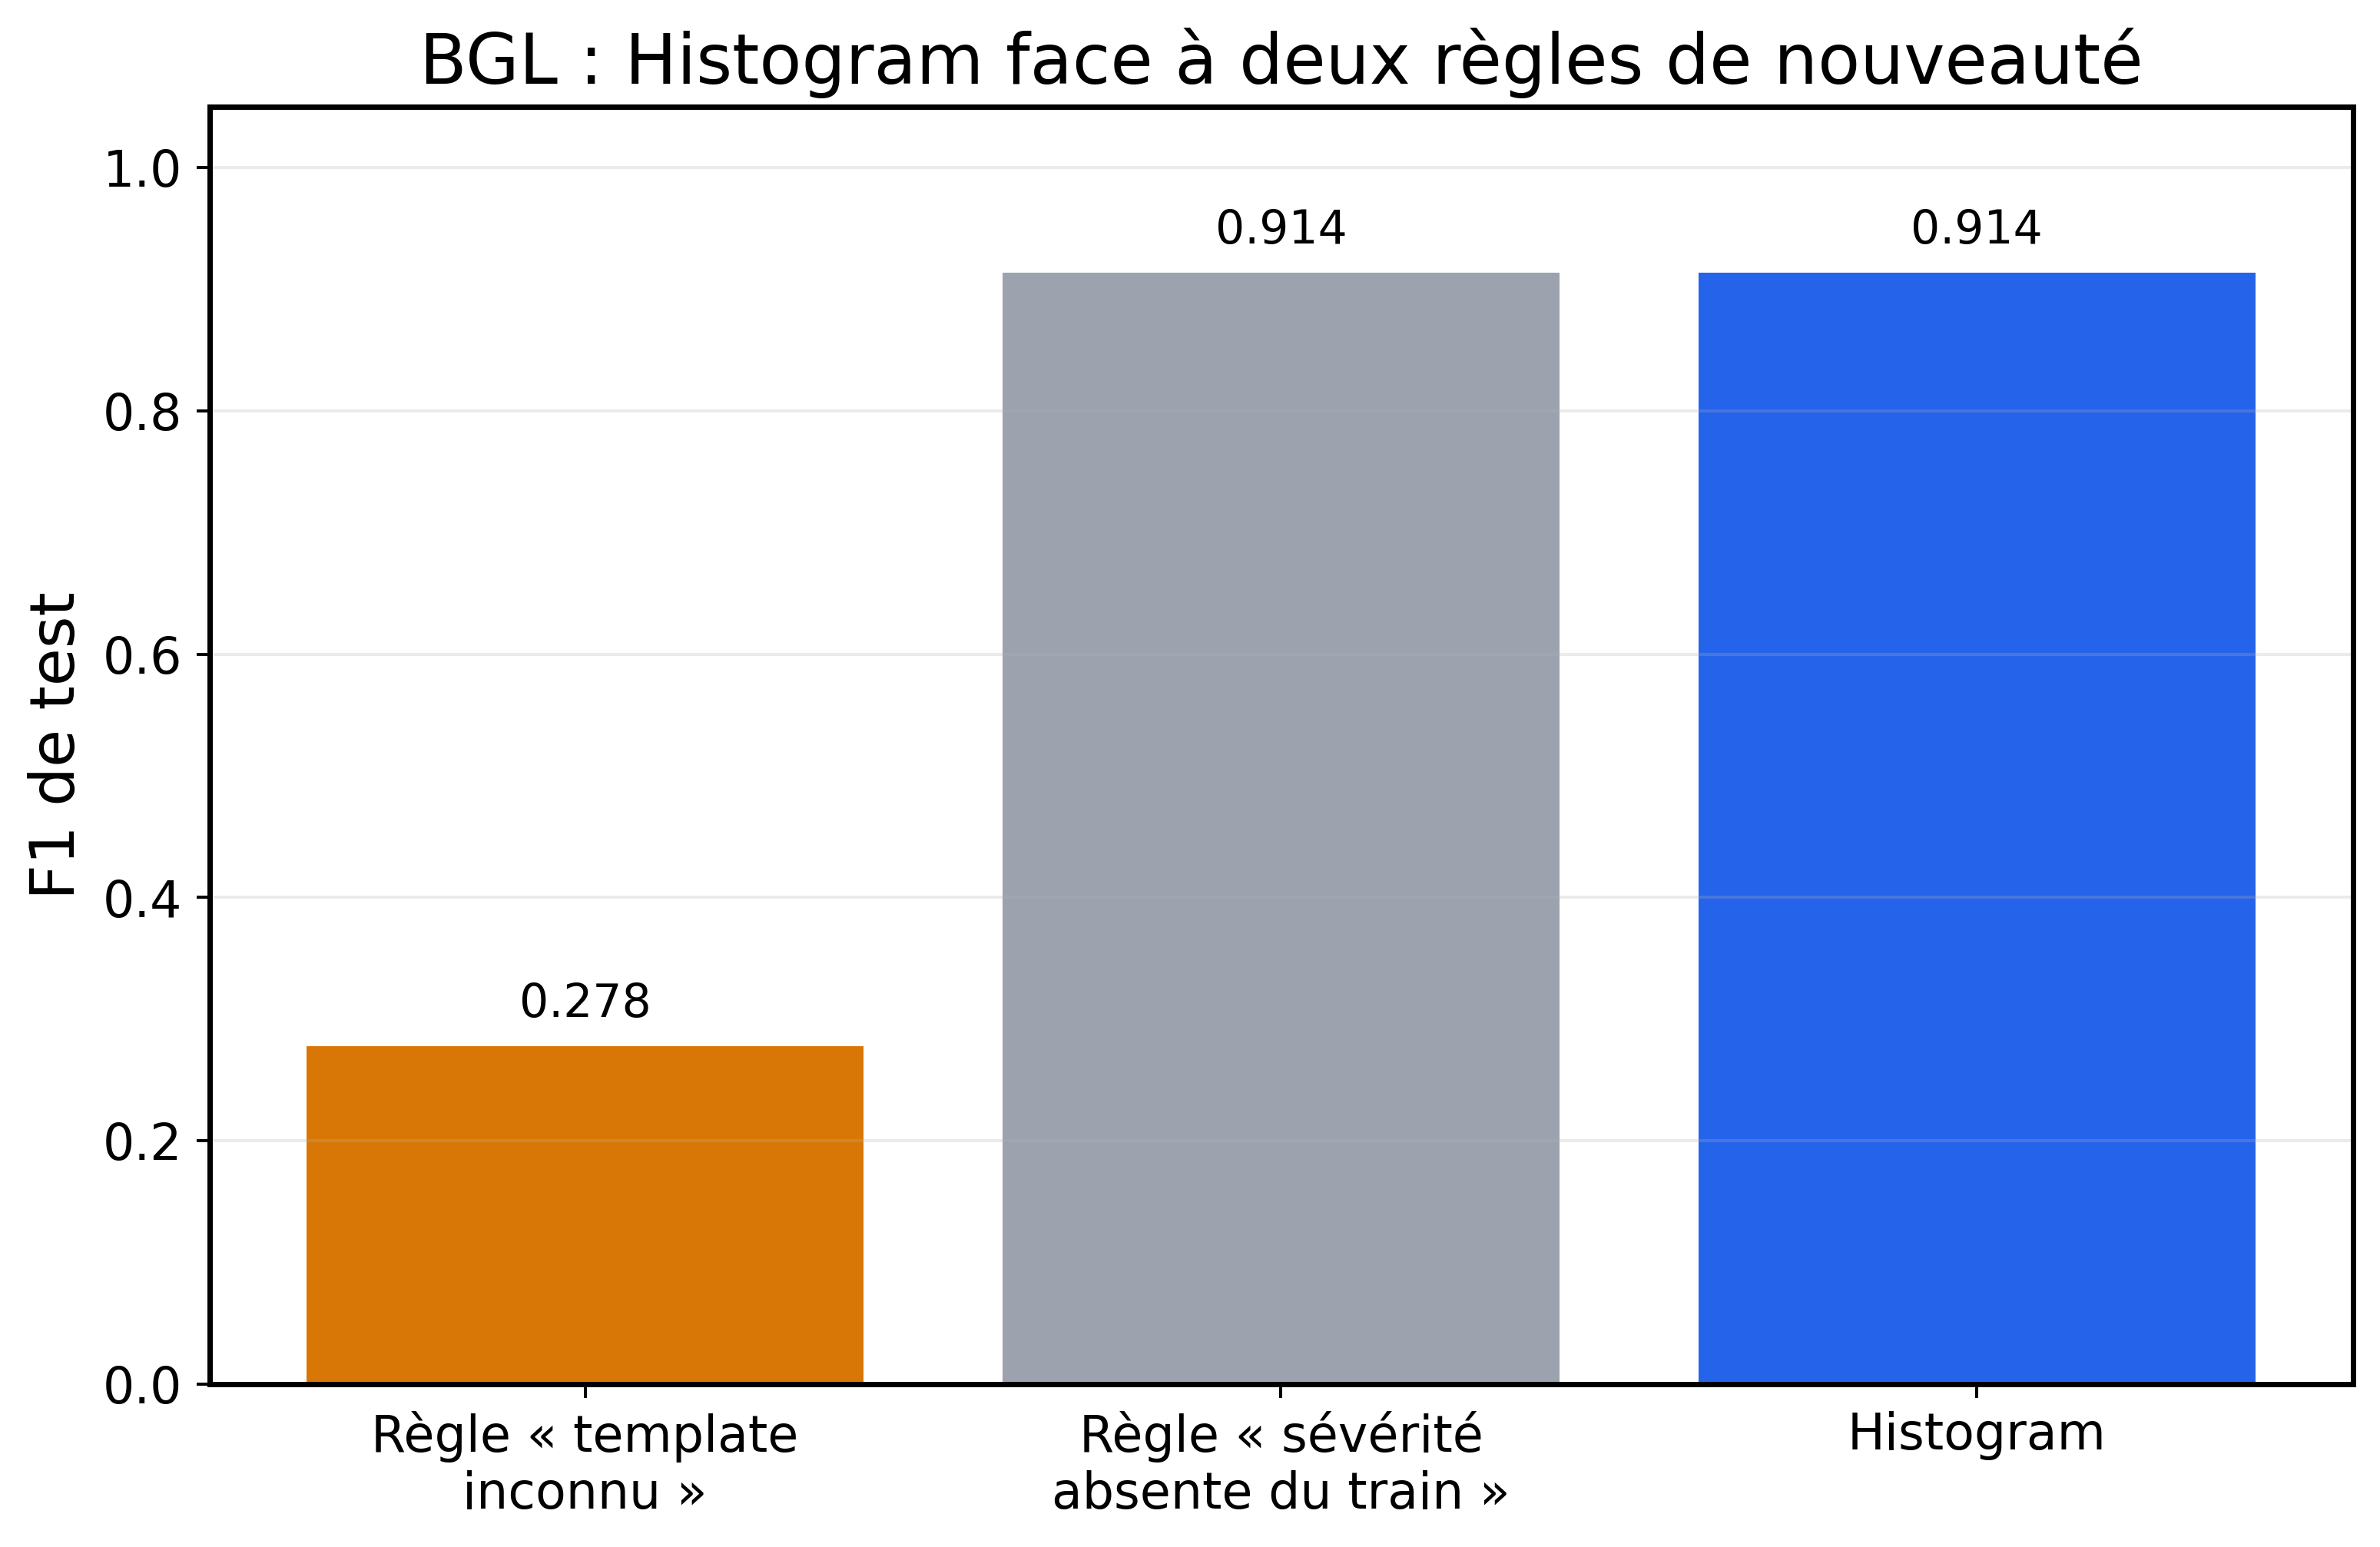
\includegraphics[width=0.96\textwidth]{fig_bgl_histogram_vs_unknown_baseline.png}
  \caption[Histogram et deux règles de nouveauté sur BGL.]{Histogram face aux règles « template inconnu » et « sévérité absente de l'entraînement » sur BGL. Source : campagne BGL, second protocole, protocole principal.}
  \label{fig:bgl-baseline}
\end{figure}

\subsection{Variantes exploratoires}
\label{sec:bgl-second-protocol}
\label{sec:bgl-second-protocole}

Le protocole principal ne contient aucun positif sur un template connu. Huit variantes exploratoires, présentées en annexe (section~\ref{sec:annexe-variantes-bgl}), font varier l'entraînement ; l'une d'elles, le protocole contigu G, a été conçue après observation du test. Leur F1 varie de $0{,}5985$ à $0{,}9419$ : aucune valeur unique ne résume la performance sur BGL, et aucune variante ne remplace le protocole principal.

\subsection{Mise en perspective avec des résultats publiés}

Le tableau~\ref{tab:baselines-publiees} rappelle plusieurs scores publiés sur HDFS et BGL avec leur protocole. Ils ne forment pas un classement direct : l'unité évaluée, le fenêtrage, la taille et la prévalence du test, la partition et l'usage des labels diffèrent selon les travaux.

\begin{table}[H]
\centering
\caption[Résultats publiés sur HDFS et BGL.]{Scores F1 publiés sur HDFS et BGL, accompagnés de leur protocole. Sources : articles cités et artefacts du présent travail.}
\label{tab:baselines-publiees}
\scriptsize
\begin{tabularx}{\textwidth}{p{2.25cm}p{0.80cm}p{1.85cm}p{1.8cm}Xr}
\toprule
\textbf{Source} & \textbf{Jeu} & \textbf{Méthode} & \textbf{Cadre} & \textbf{Unité et partition} & \textbf{F1} \\
\midrule
DeepLog \cite{du2017deeplog} & HDFS & DeepLog & semi-supervisé & session ; $4\,855$ sessions normales au train & 0,96 \\
LogBERT \cite{guo2021logbert} & HDFS & LogBERT & auto-supervisé & session ; environ $5\,000$ séquences normales & 0,8232 \\
LogBERT \cite{guo2021logbert} & HDFS & Isolation Forest & non supervisé & même protocole & 0,6049 \\
LogBERT \cite{guo2021logbert} & BGL & LogBERT & auto-supervisé & fenêtre de 5 min & 0,9083 \\
LogBERT \cite{guo2021logbert} & BGL & Isolation Forest & non supervisé & fenêtre de 5 min & 0,3065 \\
Le et Zhang \cite{le2022logbased} & HDFS & DeepLog & semi-supervisé & session ; partition aléatoire 80:20 & 0,908 \\
Le et Zhang \cite{le2022logbased} & HDFS & LogRobust & supervisé & session ; partition aléatoire 80:20 & 0,980 \\
Le et Zhang \cite{le2022logbased} & BGL & DeepLog & semi-supervisé & fenêtre d'une heure ; aléatoire / chronologique & 0,927 / 0,426 \\
Le et Zhang \cite{le2022logbased} & BGL & LogRobust & supervisé & fenêtre d'une heure ; aléatoire / chronologique & 0,981 / 0,967 \\
\midrule
Ce travail & HDFS & Histogram, moyenne & score sans label, seuil validé & bloc ; chronologique 60/20/20, test complet & 0,8684 \\
Ce travail & BGL & Histogram & nouveauté, seuil validé & événement ; trois périodes chronologiques & 0,9137 \\
\bottomrule
\end{tabularx}
\end{table}

Le F1 HDFS de $0{,}8684$ se situe dans l'ordre de grandeur de plusieurs résultats publiés, sans leur être directement comparable. La sensibilité au protocole observée ici rejoint celle rapportée par Le et Zhang : sur BGL, le F1 de DeepLog passe de $0{,}927$ à $0{,}426$ lorsque la partition devient chronologique \cite{le2022logbased}. Un contrôle Isolation Forest strict atteint pour sa part un F1 moyen de $0{,}2045$ au niveau événement sur HDFS et de $0{,}2535$ sur BGL, ce dernier niveau étant voisin de la prédiction systématiquement positive ($0{,}2531$).

\section{CSE-CIC-IDS2018 : audit de deux journées}
\label{sec:csecic-resultats}

Les fichiers du 15 et du 16 février 2018 ont été retéléchargés depuis la source vérifiée par l'auteur ; leurs empreintes SHA-256 sont identiques à celles des copies employées par les campagnes. Cet audit porte néanmoins sur deux journées seulement et ne constitue pas une évaluation générale de CSE-CIC-IDS2018. L'entraînement utilise le 15 février et le test le 16. Sur cinq graines, avec des échantillons équilibrés de $20\,000$ lignes par journée et 78 caractéristiques, la régression logistique atteint un F1 moyen de $0{,}9992$, contre $0{,}4014$ pour le Random Forest.

À la prévalence observée, une expérience complémentaire tire les lignes indépendamment de leur étiquette et compare les deux directions de transfert. Le tableau~\ref{tab:csecic-prevalence} montre que le résultat favorable du 15 vers le 16 repose principalement sur le port de destination.

\begin{table}[H]
\centering
\caption{CSE-CIC-IDS2018 à prévalence observée, F1 moyen sur cinq graines.}
\label{tab:csecic-prevalence}
\small
\begin{tabular}{llrr}
\toprule
\textbf{Direction} & \textbf{Variables} & \textbf{LR} & \textbf{RF} \\
\midrule
15 $\rightarrow$ 16 & 78 & 0,9943 & 0,0959 \\
15 $\rightarrow$ 16 & sans \texttt{Dst Port} & 0,7284 & 0,0713 \\
15 $\rightarrow$ 16 & \texttt{Dst Port} seul & 0,9997 & 0,8692 \\
16 $\rightarrow$ 15 & 78 & 0,2342 & 0,1440 \\
intra 15 & 78 & 0,9897 & 0,9986 \\
intra 16 & 78 & 0,9999 & 1,0000 \\
\bottomrule
\end{tabular}
\end{table}

Une règle fixe qui déclare attaque tout flux dont le port de destination est inférieur à 1024 atteint elle aussi $0{,}9997$ sur le 16 février, mais seulement $0{,}1215$ sur le 15. Le transfert inverse ne dépasse pas $0{,}2342$. La régression logistique exploite donc un raccourci propre à la journée de test plutôt qu'une signature générale des attaques. Le Random Forest n'est pas intrinsèquement faible : il atteint $0{,}9986$ et $1{,}0000$ en intra-journée, mais n'extrapole pas du port 80, vu le 15 février, au port 21 de SlowHTTPTest le 16. Les fichiers vérifiés s'arrêtent par ailleurs à une limite de lignes compatible avec une exportation par tableur ; cette propriété de la distribution est conservée comme limite du corpus, sans remettre en cause sa provenance.

\section{Routeur open-set}

Le jeu de calibration contient 31 fichiers répartis en neuf groupes : 28 connus et 3 inconnus. Sans seuil, le routeur classe correctement tous les connus mais ne rejette aucun inconnu. Le seuil de score principal est calibré sur les seules sources connues, puis gelé. À 100, les trois inconnus sont rejetés (intervalle exact à 95~\% : $[0{,}292\,;\,1]$, que la faiblesse de l'effectif rend très large) et aucun des 28 connus ne l’est ($[0\,;\,0{,}123]$).

Le seuil gelé est également appliqué, sans recalibration, à 37 fichiers locaux dont l’étiquette est fixée avant le routage : 17 inconnus relevant de 15 schémas (tables CSV génériques, audit Solaris BSM et listes de sessions de l'évaluation DARPA 1998), 18 connus issus de sources non vues à la calibration, et 2 fichiers ambigus, exclus des taux. Sur les 66 fichiers non ambigus (31 de calibration et 35 supplémentaires), $20/20$ inconnus sont rejetés ($[0{,}832\,;\,1]$) et $3/46$ connus le sont à tort ($[0{,}014\,;\,0{,}179]$) : deux journées CSE-CIC-IDS2018 et la forme structurée de Linux\_2k. Les 43 fichiers connus acceptés sont tous correctement orientés.

\begin{figure}[H]
  \centering
  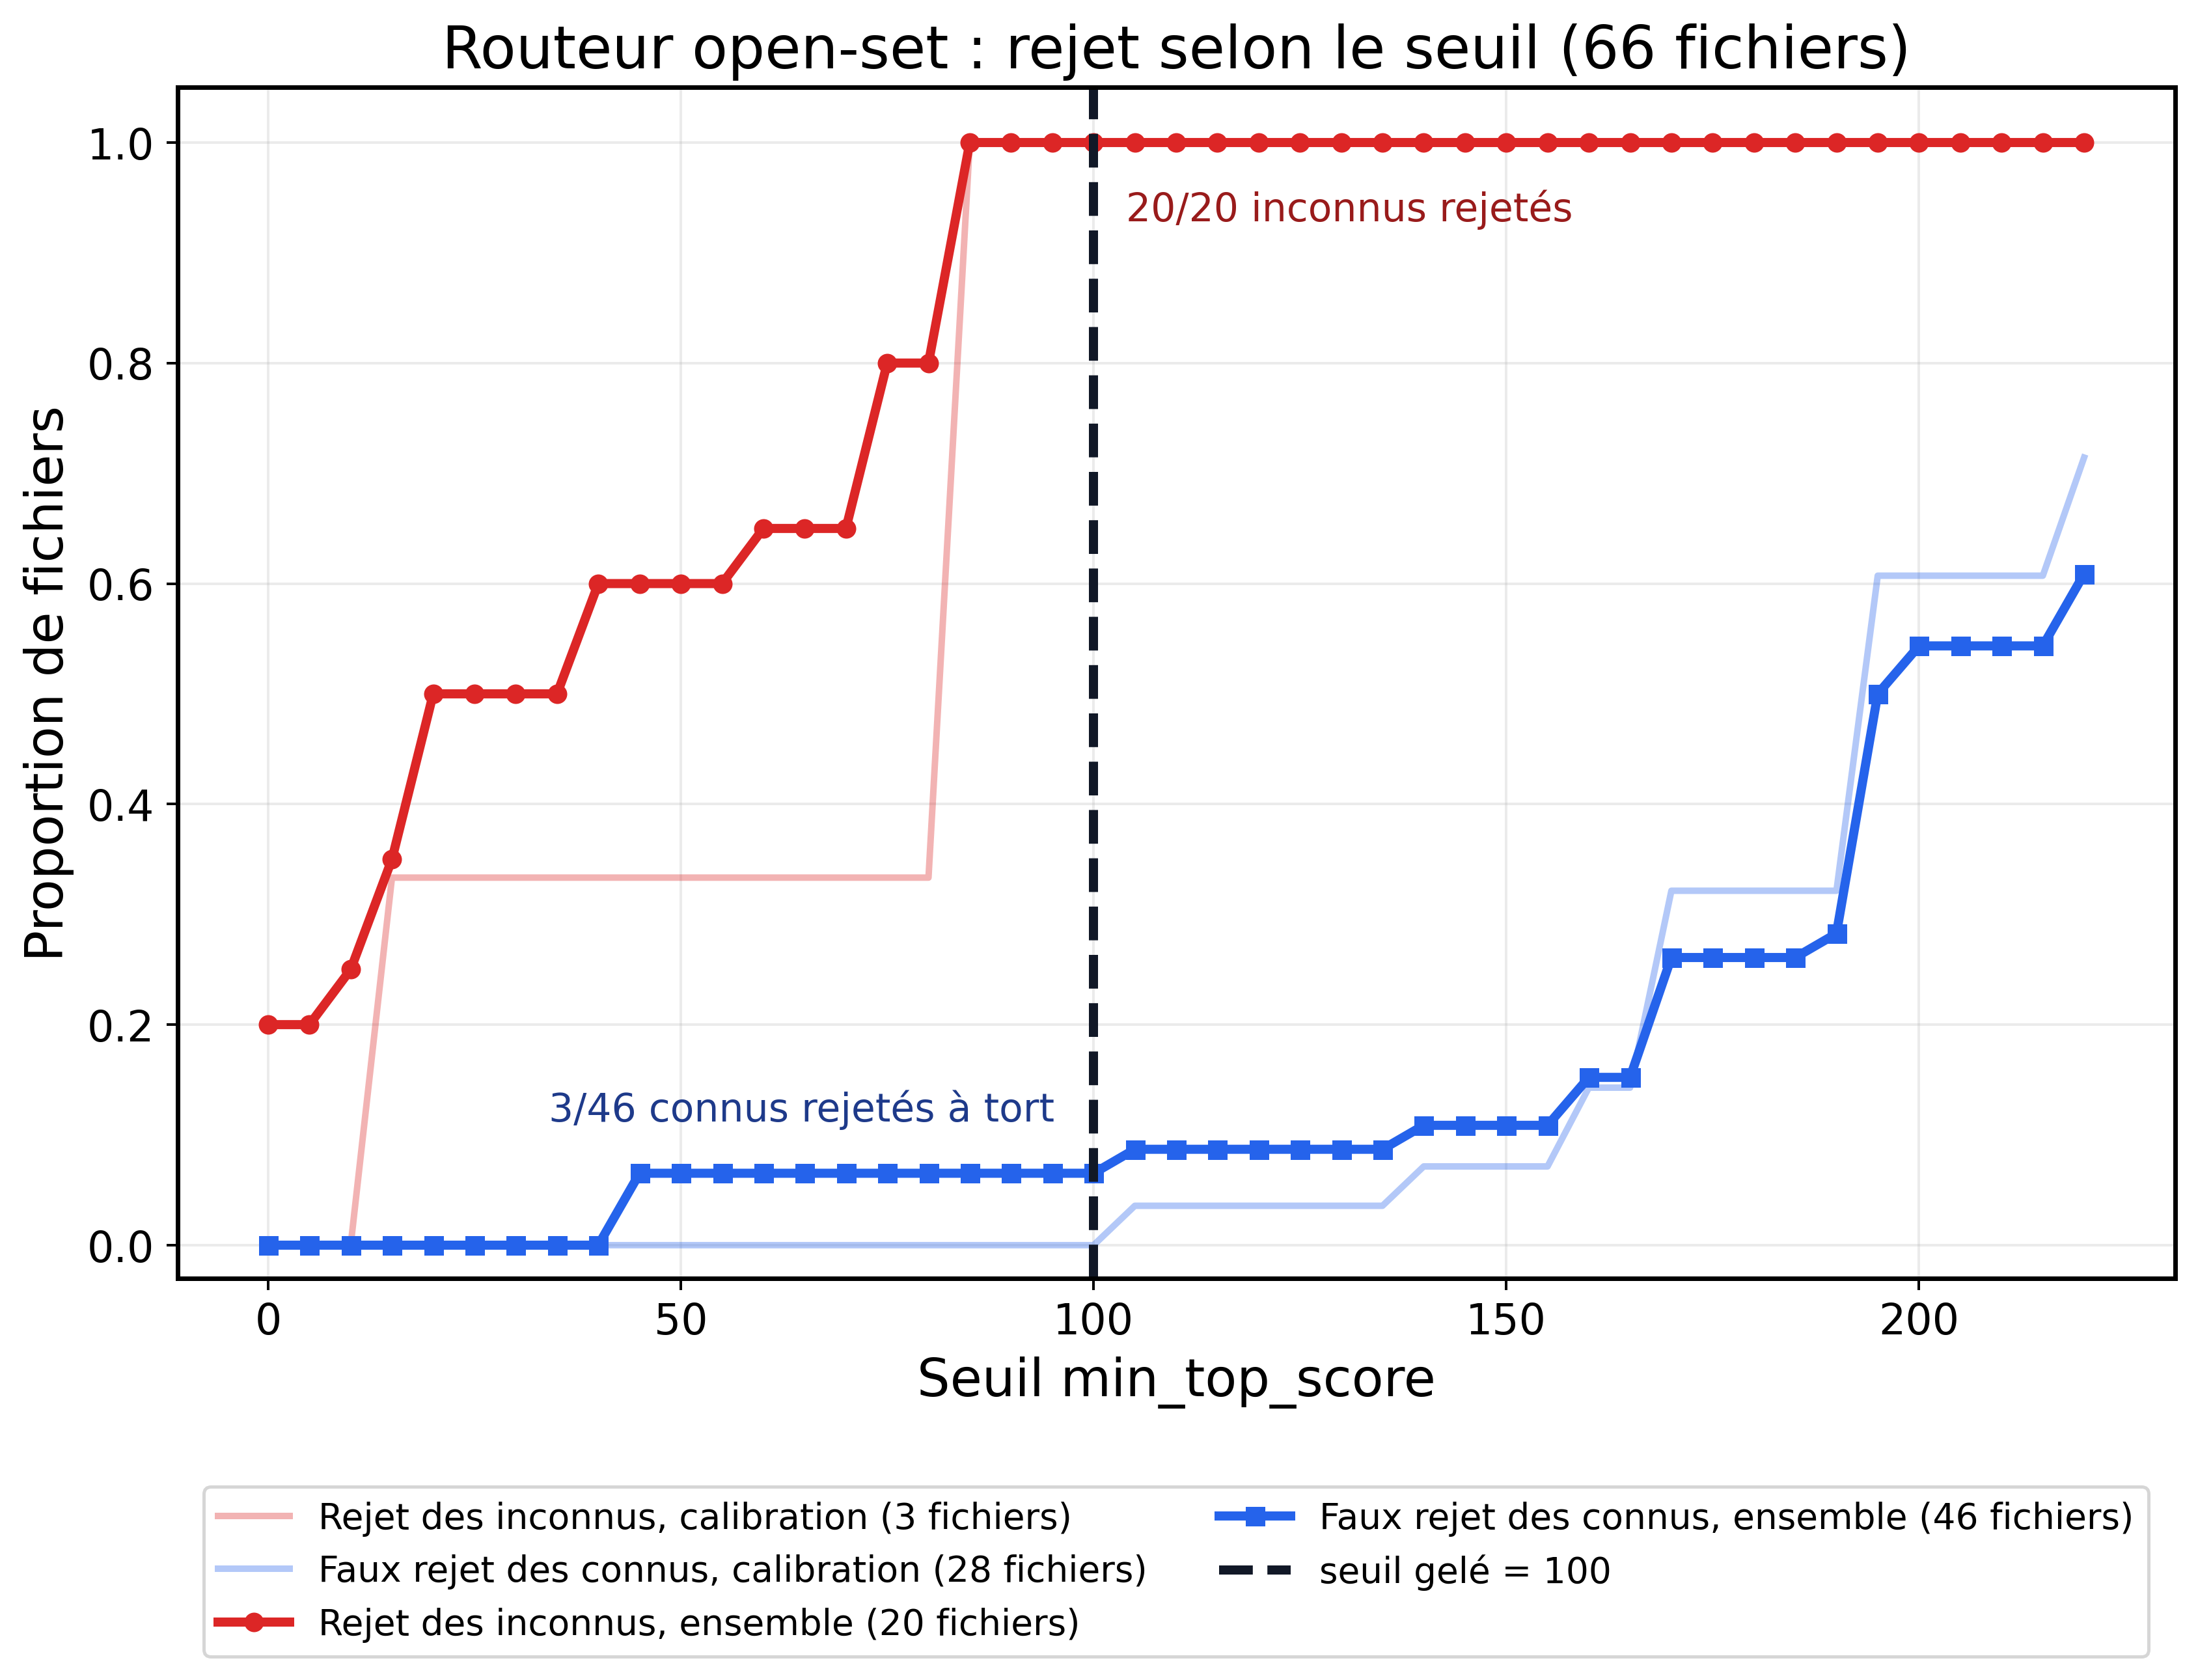
\includegraphics[width=0.97\textwidth]{fig_router_open_set_tradeoff.png}
  \caption[Rejet open-set du routeur selon le seuil, sur les 31 fichiers de calibration et les 66 fichiers.]{Rejet des inconnus et faux rejet des connus selon le seuil, sur les 31 fichiers de calibration et sur l'ensemble des 66 fichiers. Le seuil 100 a été fixé sur la calibration puis gelé ; le balayage est un diagnostic a posteriori. Source : évaluation open-set du routeur.}
  \label{fig:routeur-open-set}
\end{figure}

Pour les journaux texte, les scores du routeur reprennent les colonnes \texttt{dataset} et \texttt{subtype} produites par le parseur de format : le rejet des inconnus mesure donc en partie la capacité de ce parseur à ne pas reconnaître un format, et non une décision indépendante (section~\ref{sec:limites}). Le seuil gelé écarte en outre des sources connues dont le schéma n’a pas été vu à la calibration. Cette mesure porte sur le routage des sources, pas sur l'avantage prédictif des modèles sélectionnés.

\section{Spécialisation des modèles}
\label{sec:e-h3b}

Un protocole versionné avant son exécution compare un modèle commun aux trois familles à un modèle propre à chacune, avec le même espace de 17 variables et les mêmes hyperparamètres. Les familles sont CICIDS2017, UNSW-NB15 et Linux/auth ; ce dernier est un jeu public synthétique, généré avec la bibliothèque Faker et diffusé sur Kaggle, de sorte que ses résultats ne valent pas pour des journaux réels. Pour chaque famille, chaque catégorie d'attaque est tour à tour absente de l'entraînement, puis testée avec autant de lignes normales, à raison d'au plus $1\,500$ positifs par test, soit 18 catégories et cinq graines. Le test étant équilibré, la prédiction systématiquement positive atteint un F1 de $0{,}6667$. Le modèle spécialisé reçoit la famille correcte ; cette condition oracle ne teste donc pas le classifieur de routage. Le critère de non-infériorité exige, pour chaque famille, une borne inférieure de l'IC apparié à 95~\% d'au moins $-0{,}01$. L'intervalle est calculé sur les moyennes par graine et par famille, soit cinq valeurs appariées par famille ; les cinq graines partagent les mêmes fichiers sources.

\paragraph{Contenu de l'espace commun.} Les 17 variables sont treize grandeurs numériques et quatre catégorielles (protocole, service, état, statut). Elles ne désignent pas la même chose d'une famille à l'autre. Le port source vaut zéro pour les trois familles. Chaque famille ne renseigne qu'une partie des autres variables et met les autres à zéro ou à vide : la durée, les paquets, les octets et le débit pour les flux réseau ; les tentatives, l'heure et le jour pour Linux/auth ; le port de destination pour CICIDS2017 et Linux/auth seulement. Les quatre résumés numériques (moyenne, écart-type, maximum, part de valeurs non nulles), seules variables renseignées partout, sont calculés sur l'ensemble des colonnes d'origine pour les flux et sur quatre colonnes pour Linux/auth. L'espace commun juxtapose donc des sous-espaces propres à chaque famille ; le motif des zéros suffit à reconnaître la famille. La comparaison mesure ainsi l'effet d'un modèle séparé par famille face à un modèle unique sur cette juxtaposition, non la valeur d'une représentation partagée, qui n'existe pas ici. Elle reste pertinente pour H3, dont la seconde clause porte précisément sur ce choix d'architecture : faut-il un modèle par famille, ou un modèle unique suffit-il ? Comme la famille est reconnaissable par le modèle commun, un modèle unique dispose en principe de la même information qu'un modèle spécialisé ; séparer les modèles ne peut alors apporter qu'une capacité propre à chaque famille. Le résultat se lit dans ce sens : sur CICIDS2017, le modèle spécialisé n'est pas établi non inférieur au modèle commun, et la séparation n'y apporte rien de démontré.

\begin{table}[H]
\centering
\small
\caption{Modèle spécialisé et modèle commun, catégorie d'attaque tenue à l'écart, cinq graines appariées.}
\label{tab:e-h3b-family-models}
\begin{tabularx}{\textwidth}{XrrrXl}
\toprule
\textbf{Famille} & \textbf{F1 commun} & \textbf{F1 spécialisé} & \textbf{$\Delta$ F1} & \textbf{IC à 95~\% de $\Delta$} & \textbf{Critère} \\
\midrule
CICIDS & 0,1349 & 0,1514 & $+0{,}0165$ & [$-0{,}0190$ ; $0{,}0520$] & échoué \\
Linux/auth & 0,0528 & 0,2197 & $+0{,}1669$ & [$0{,}1081$ ; $0{,}2256$] & satisfait \\
UNSW & 0,7817 & 0,7910 & $+0{,}0093$ & [$0{,}0050$ ; $0{,}0135$] & satisfait \\
\bottomrule
\end{tabularx}
\end{table}

La non-infériorité globale n'est pas établie, car l'intervalle de CICIDS descend sous la marge. Cet échec tient à l'imprécision de l'estimation et non à un delta défavorable. Sur Linux/auth et UNSW, l'intervalle exclut zéro en faveur du modèle spécialisé. L'écart de Linux/auth provient surtout d'une catégorie, \texttt{port\_scan} ($0{,}7100$ contre $0{,}0675$) ; les variables \texttt{status} et \texttt{service}, qui en font partie, peuvent y servir de mandataires de l'étiquette dans ce corpus généré. Le niveau absolu reste le résultat principal : sur CICIDS et Linux/auth, les deux modèles restent très en dessous de la prédiction systématiquement positive, et le F1 vaut zéro pour Bot, Infiltration et \texttt{brute\_force}. UNSW dépasse ce niveau en moyenne, mais pas sur Fuzzers ($0{,}3391$). Spécialiser le modèle ne corrige donc pas la fragilité face à une attaque absente de l'entraînement. Les effectifs d'Infiltration (72 lignes de test) et de Worms (348) rendent leurs scores peu précis.

Une référence par séparation aléatoire stratifiée, sur les mêmes données chargées sans fuite de l'étiquette, donne des F1 spécialisés de $0{,}9904$ (CICIDS), $0{,}8157$ (Linux/auth) et $0{,}9035$ (UNSW), et satisfait le critère pour les trois familles. L'écart avec le tableau~\ref{tab:e-h3b-family-models} mesure le coût du retrait d'une catégorie. Une comparaison antérieure, en séparation aléatoire, est écartée pour un défaut de chargement (section~\ref{sec:limites}). Aucune de ces expériences n'établit la qualité du routeur ni la généralisation à une famille absente.

\section{Couverture multiformat}

La campagne de couverture multiformat est un test d’intégration des adaptateurs. Elle vise $1\,000$ unités par source. Sept sources fournissent $7\,000$ unités, dont Linux/auth, jeu public entièrement synthétique ; Apache n’est représenté que par une fixture synthétique d’une ligne, faute de corpus Apache réel disponible localement. Au total, $7\,001$ unités, dont cette ligne, sont lues et émises dans le schéma commun sans erreur d’exécution ni perte enregistrée.

\begin{figure}[H]
  \centering
  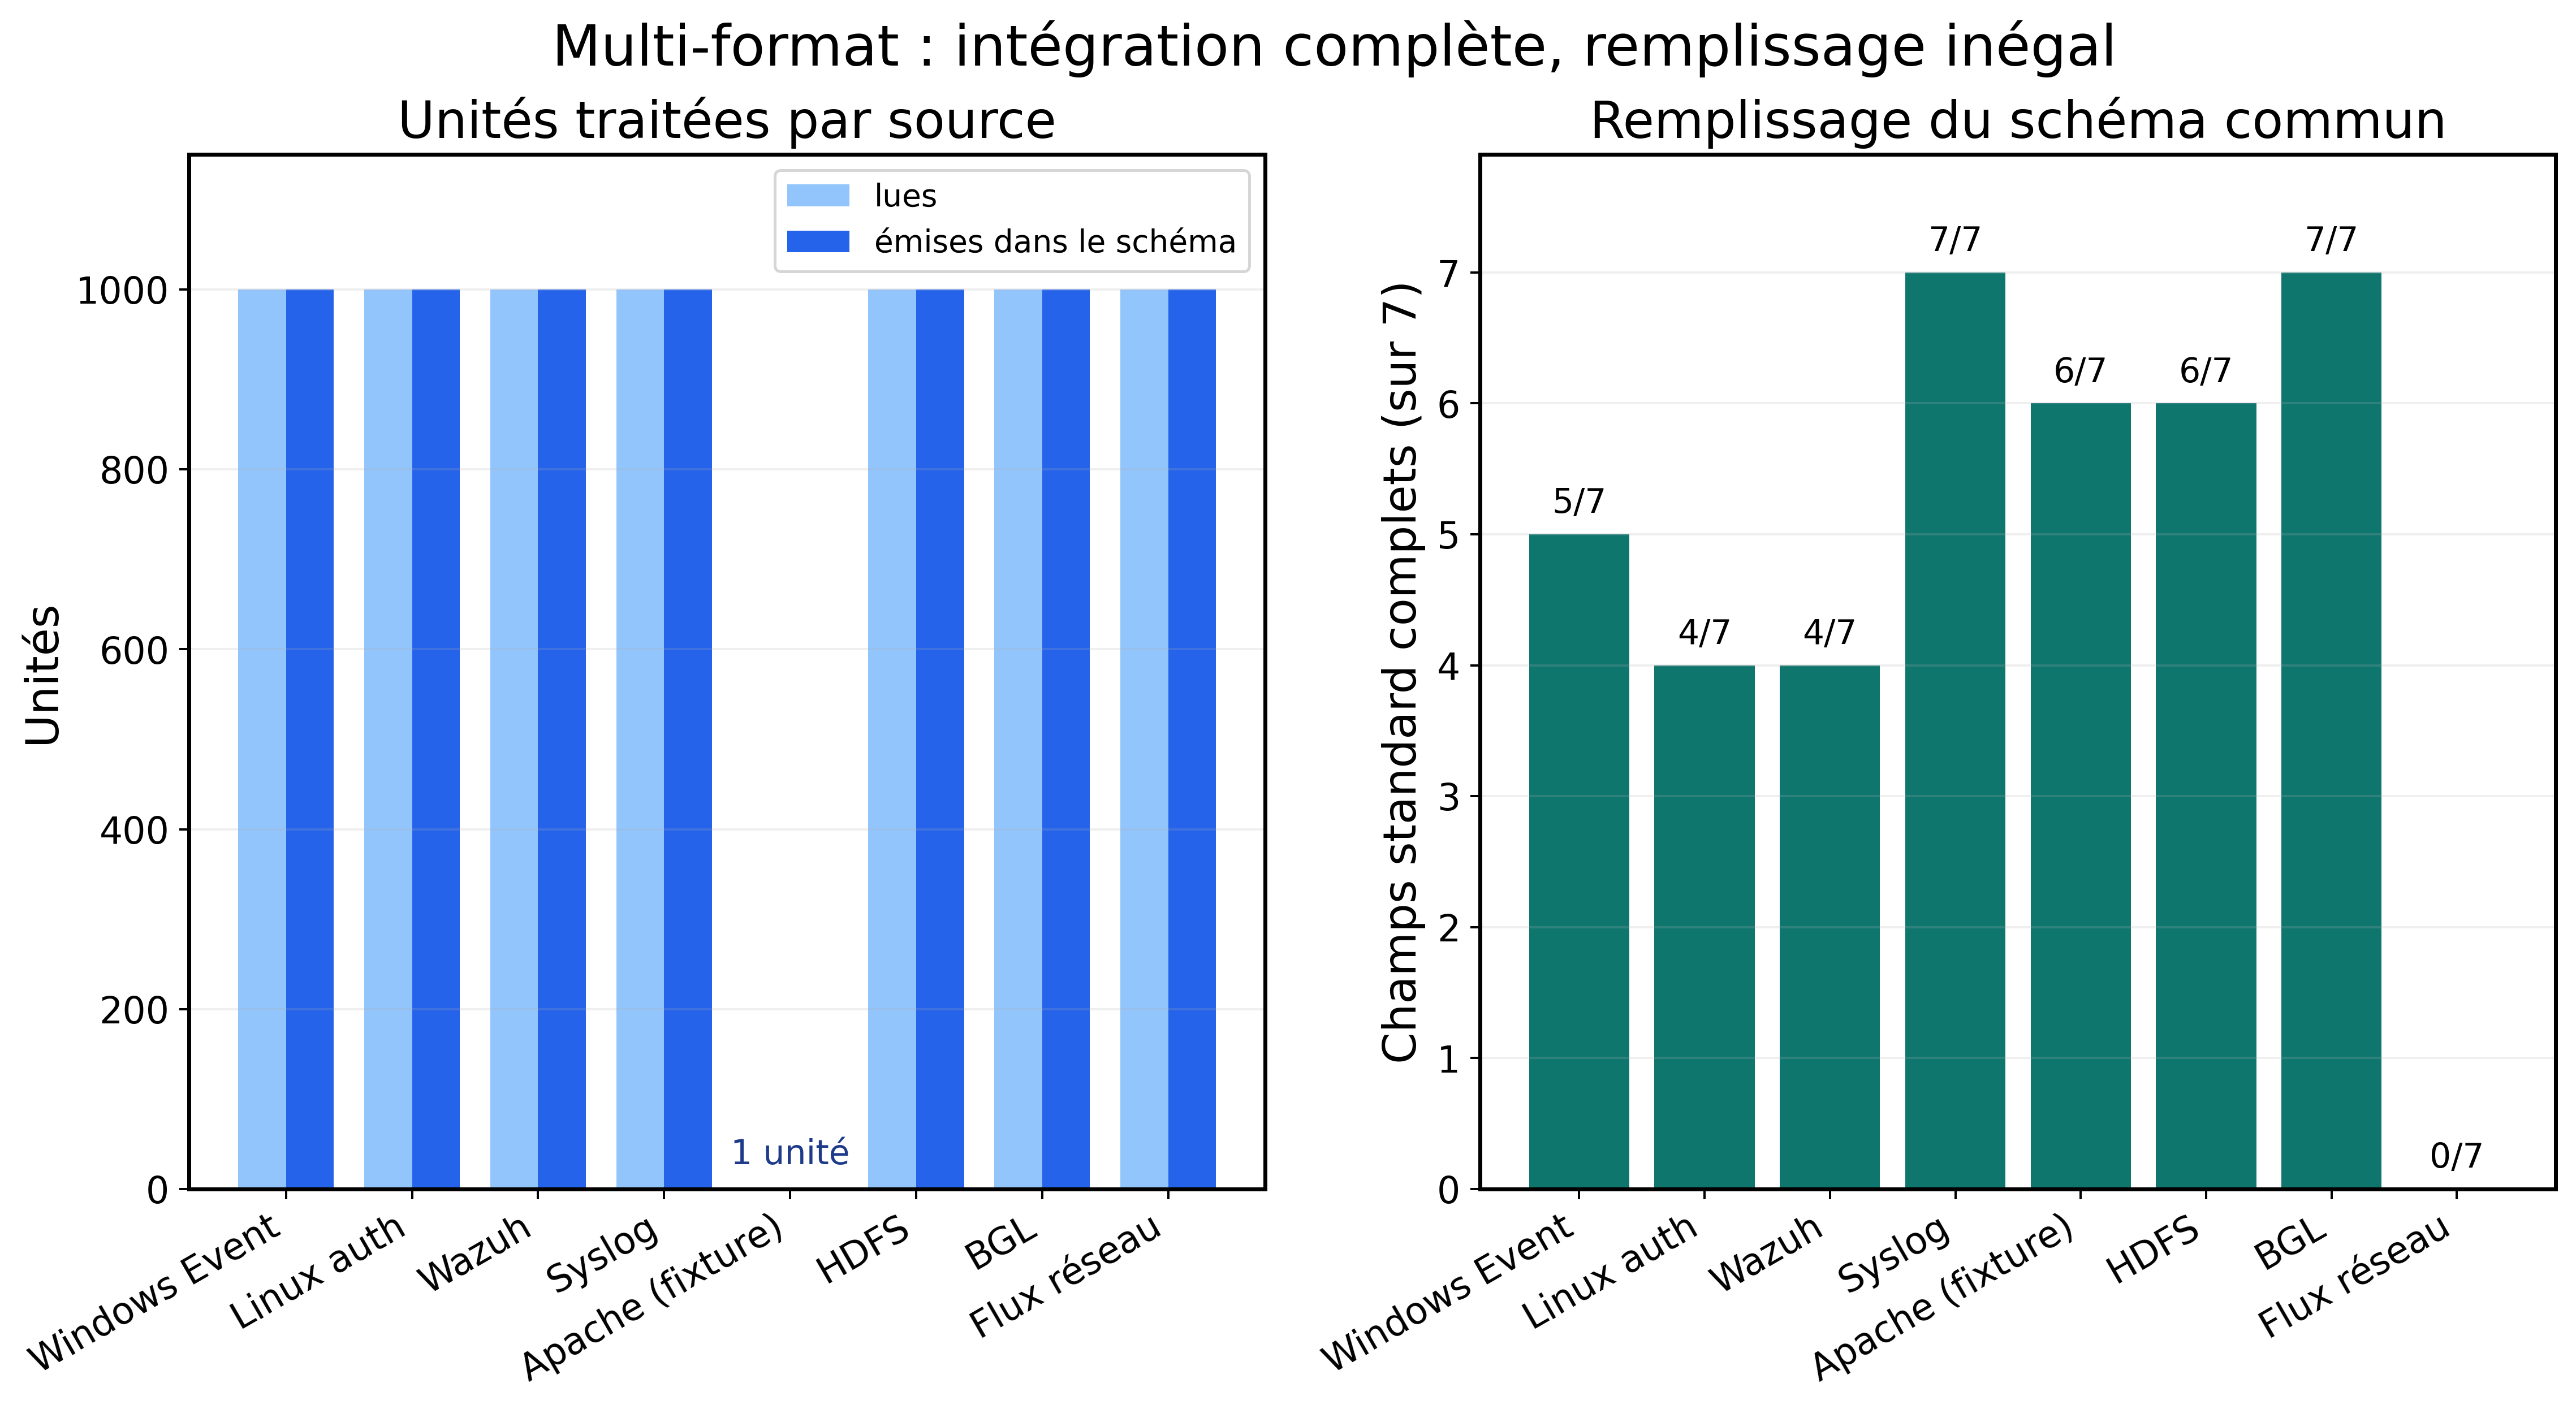
\includegraphics[width=0.98\textwidth]{fig_multiformat_coverage_by_source.png}
  \caption[Couverture et remplissage du schéma par source.]{Unités lues et émises dans le schéma commun, et nombre de champs standard complets, par source. Source : campagne de couverture multiformat.}
  \label{fig:couverture-multiformat}
\end{figure}

La campagne établit donc une propriété d’intégration : chaque unité présente dans le protocole produit une ligne, sans erreur d’exécution. Elle n'établit pas la fidélité sémantique de la normalisation : le remplissage du schéma commun varie de sept champs standard sur sept pour syslog et BGL à aucun pour les flux réseau tabulaires. Les sept champs mesurés (horodatage, source, hôte, famille, catégorie, sévérité, message) sont ceux d'un événement de journal ; le schéma en compte davantage, dont le remplissage n'est pas mesuré. Le score nul des flux ne tient pas aux données : la voie de préparation des flux ne projette aucune colonne vers ces champs, alors que CSE-CIC-IDS2018 fournit par exemple un horodatage, un port de destination et un protocole. Il mesure une lacune de l'adaptateur, non une limite intrinsèque des flux réseau. Un adaptateur de flux, ajouté et testé ensuite, projette les colonnes présentes vers les champs réseau du schéma ; il a été appliqué, sous un protocole versionné avant son exécution, aux 1~000 premières lignes de chacun des dix fichiers de flux locaux. Sur les sept champs réseau mesurés (horodatage, adresses et ports source et destination, protocole, octets émis), les huit fichiers CICIDS2017 en remplissent deux, le port de destination et les octets, et les deux fichiers CSE-CIC-IDS2018 quatre, avec l'horodatage et le protocole ; aucune valeur de l'étiquette n'apparaît dans un champ normalisé. Les champs restés vides, adresses IP, port source, sévérité et message, sont absents de ces exports : ce qui manque désormais tient aux données, non à l'adaptateur. Aucun incident n'est par ailleurs analysé conjointement à partir de sources système et réseau.

\section{Benchmark des architectures A--D}

Le benchmark compare quatre architectures : A, monolithe ; B, workers centralisés ; C, agents autonomes avec mémoire désactivée ; D, agents autonomes avec mémoire activée. Les charges sont 100, 500, $1\,000$ et $5\,000$ tâches. Chaque combinaison est répétée dix fois, soit 160 exécutions et $264\,000$ traitements. Aucun échec n’est enregistré. Les tâches sont des microtâches synthétiques, presque sans travail utile : le benchmark mesure le coût fixe de l'orchestration.

\paragraph{Machine de test.} Le benchmark et les campagnes locales s'exécutent sur un ordinateur portable non dédié : processeur Intel Core i5-8350U à 1,7~GHz (4 cœurs, 8 processeurs logiques), $8\,425\,529\,344$ octets de mémoire (7,8~Gio), Windows. Le benchmark A--D a été exécuté avec Python 3.11.9 ; les campagnes de contrôle de novembre 2026 avec Python 3.12.3, et celles qui appellent un modèle avec scikit-learn 1.8.0 et NumPy 2.4.5. Ces valeurs sont inscrites dans les manifestes d'environnement des campagnes. Redis 7.4.9 s'exécute dans un conteneur Docker sur le même hôte. Aucun cœur n'est réservé et la gestion d'énergie n'est pas désactivée : les débits absolus dépendent de cette machine, et seuls les rapports entre architectures mesurés dans une même exécution sont comparés.

\begin{figure}[H]
  \centering
  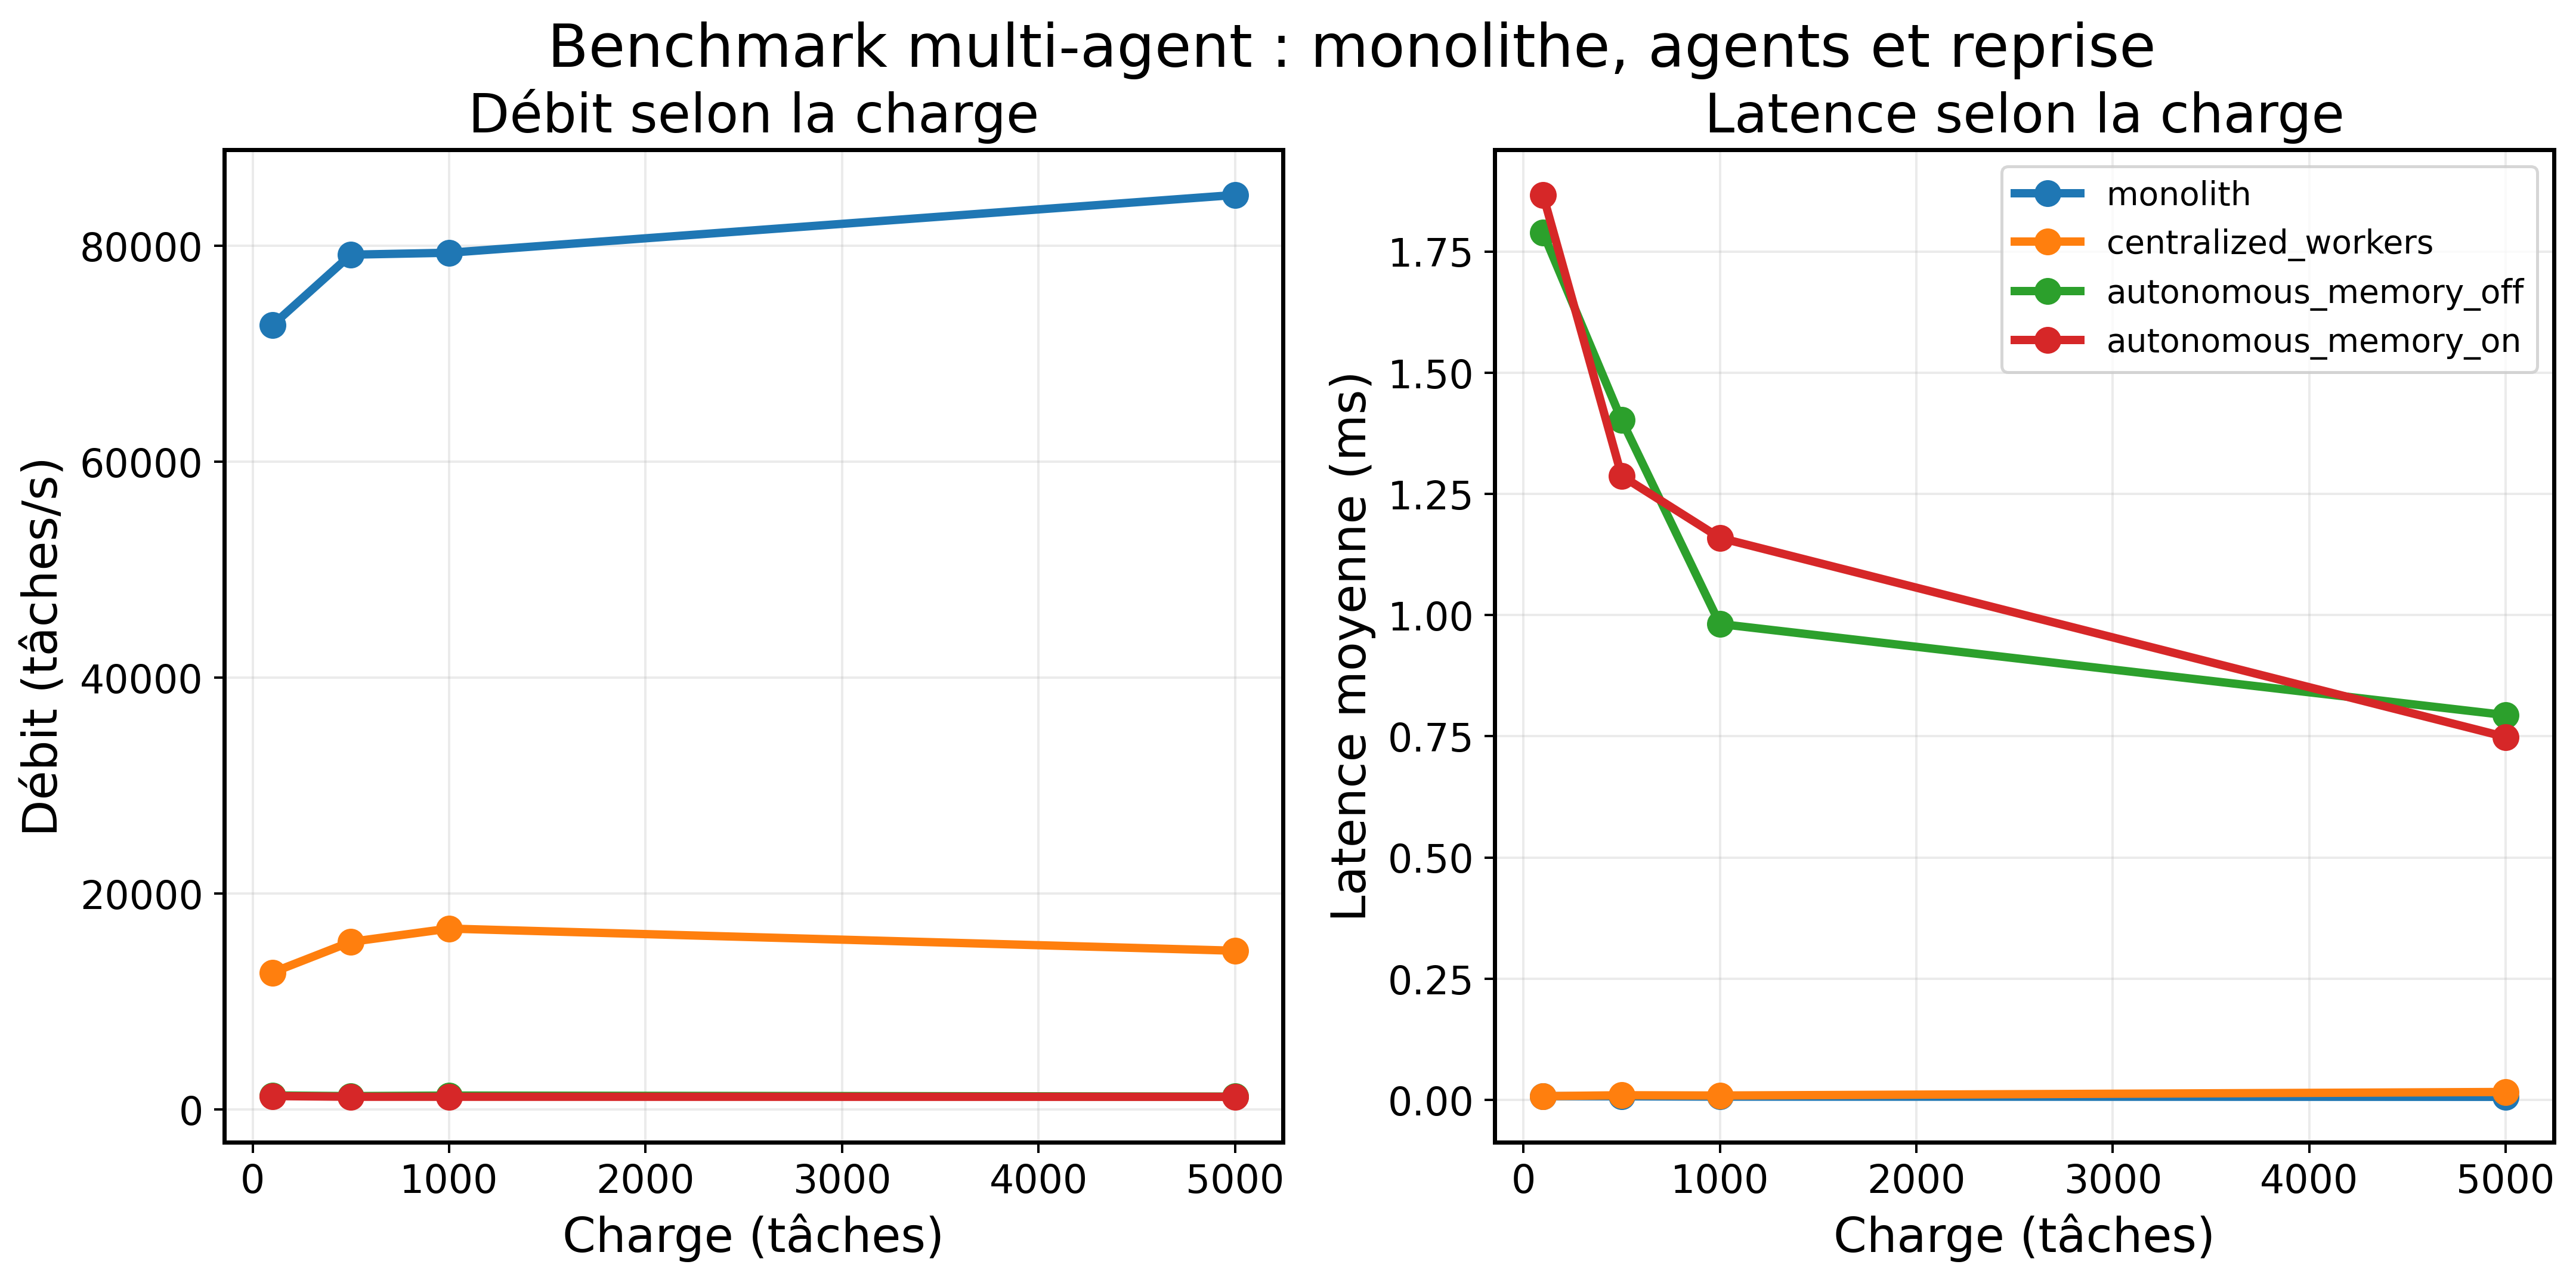
\includegraphics[width=0.99\textwidth]{fig_multi_agent_throughput_latency.png}
  \caption[Débit et latence des architectures A--D selon la charge.]{Débit et latence moyenne des architectures A--D selon la charge. Source : benchmark A--D.}
  \label{fig:benchmark-abcd}
\end{figure}

Le débit est exprimé en tâches par seconde et la latence en millisecondes. Le temps CPU est enregistré en secondes de processus et la mémoire comme pic de \emph{resident set size} ; ces mesures de processus local ne sont pas des consommations énergétiques.

\begin{table}[H]
\centering
\caption{Débit moyen du benchmark A--D (tâches/s) et IC à 95~\%, dix répétitions, charges extrêmes.}
\label{tab:benchmark-debit}
\small
\resizebox{\textwidth}{!}{%
\begin{tabular}{rcccc}
\toprule
\textbf{Charge} & \textbf{A, monolithe} & \textbf{B, workers} & \textbf{C, agents} & \textbf{D, agents + mémoire} \\
\midrule
100 & $72\,657$ [$56\,283$ ; $89\,030$] & $12\,694$ [$10\,762$ ; $14\,626$] & $1\,309$ [$1\,103$ ; $1\,514$] & $1\,249$ [$1\,094$ ; $1\,404$] \\
$5\,000$ & $84\,728$ [$79\,652$ ; $89\,803$] & $14\,714$ [$13\,059$ ; $16\,368$] & $1\,201$ [$1\,124$ ; $1\,278$] & $1\,178$ [$1\,124$ ; $1\,232$] \\
\bottomrule
\end{tabular}
}
\end{table}

Aux quatre charges, le monolithe traite 55 à 72 fois plus de tâches par seconde que les architectures à agents, et les workers centralisés une dizaine de fois plus. Sur ces microtâches, le coût d'orchestration domine entièrement le travail utile ; ce résultat était attendu et ne dit rien, à lui seul, du rapport qui s'établirait sur des tâches d'inférence réelles, lequel n'a pas été mesuré. Une estimation permet toutefois de situer ce coût. Le surcoût par tâche des agents sur le monolithe vaut $1/\text{débit}_{C} - 1/\text{débit}_{A}$, soit de $0{,}75$ à $0{,}84$~ms selon la charge et l'architecture. Rapporté à la latence moyenne d'inférence de la condition M, $105{,}5$~ms (section~\ref{sec:inference-e2e}), il représenterait de $0{,}71$ à $0{,}79\,\%$ de la durée d'une tâche réelle. Ce calcul suppose un surcoût additif, indépendant de la durée de la tâche ; il n'a pas été vérifié par une mesure.

\paragraph{Mesure sur une inférence réelle.} Une campagne complémentaire, sous un protocole versionné avant son exécution, remplace l'effet synthétique par un appel au modèle Isolation Forest HDFS du prototype, sur un vecteur dérivé de la tâche, et mesure dans la même exécution les microtâches et ces tâches réelles (200 tâches, 10 graines, 1 puis 3 workers). Le monolithe y traite une tâche réelle en $20{,}9$~ms. En exécution séquentielle, le rapport de débit de C sur A passe de $0{,}029$ sur microtâches à $0{,}988$ [$0{,}963$ ; $1{,}013$] sur tâches réelles ; le surcoût mesuré de C vaut $0{,}28$~ms par tâche [$-0{,}31$ ; $0{,}87$], soit $1{,}3\,\%$ [$-1{,}4$ ; $4{,}0$], et celui de D $2{,}6\,\%$ [$-0{,}8$ ; $6{,}0$]. Avec trois workers, C et D restent 6~\% plus lents que le monolithe (rapports $0{,}938$ et $0{,}940$). La règle préenregistrée, qui testait si le surcoût restait additif, ne tranche pas : l'intervalle mesuré sur tâche réelle est plus large que le seuil. Cette règle comparait des débits d'exécutions distinctes, dont la variabilité, environ 1~ms par tâche, dépassait le surcoût à détecter. Une seconde campagne, versionnée avant son exécution et décidée après lecture de la première, mesure donc le surcoût à l'intérieur de chaque tâche, comme la durée totale moins la durée de l'appel au modèle, en exécution séquentielle (10 graines, 200 tâches). Le surcoût médian de C passe de $0{,}23$~ms sur microtâche à $0{,}39$~ms sur tâche réelle, celui de D de $0{,}25$ à $0{,}41$~ms ; l'écart, $0{,}15$~ms [$0{,}13$ ; $0{,}18$], reste sous la marge préenregistrée de $0{,}25$~ms : le surcoût est additif. Rapporté à l'appel au modèle, environ $19{,}8$~ms, il vaut $1{,}95\,\%$ pour C et $2{,}05\,\%$ pour D ; le monolithe, contrôle, n'ajoute que $0{,}004$~ms. Sur une inférence réelle, l'écart de 55 à 72 fois observé sur microtâches disparaît donc ; pour une inférence de 105~ms, un surcoût additif de $0{,}4$~ms représenterait environ $0{,}4\,\%$. Aucune différence appariée D $-$ C n'établit de gain de la mémoire : l'intervalle du débit contient zéro à chaque charge ($-113$ tâches/s [$-229$ ; $4$] pour $1\,000$ tâches), de même que celui de la latence p95, et l'équité diminue à 500 tâches ($-0{,}040$ [$-0{,}064$ ; $-0{,}017$]). Aucune tâche n'échouant, la mémoire ne dispose d'aucune information utile à exploiter, situation que traite la section~\ref{sec:e-h5}.

\subsection{Panne contrôlée appariée}
\label{sec:panne-appariee}

Pour comparer la robustesse, la même panne est rejouée sur les quatre architectures. Sur une charge appariée de 40 tâches et dix graines, le worker s'arrête après l'effet durable et sa persistance, avant l'émission du résultat ; la tâche est rejouée une fois sur un worker vivant, ou après redémarrage pour le monolithe. Le délai de détection de la panne, commun à toutes les architectures, n'est pas inclus dans la latence de reprise.

\begin{table}[H]
\centering
\caption[Panne après persistance et avant \texttt{RESULT}, dix répétitions par architecture.]{Panne après persistance et avant \texttt{RESULT}, dix répétitions par architecture. $^{*}$~Ablation exécutée sous protocole préenregistré, dans une exécution qui rejoue aussi les six autres lignes avec les mêmes doublons et pertes.}
\label{tab:panne-appariee}
\small
\resizebox{\textwidth}{!}{%
\begin{tabular}{lcrrr}
\toprule
\textbf{Architecture} & \textbf{Magasin d'idempotence} & \textbf{Pertes} & \textbf{Effets dupliqués} & \textbf{Reprise médiane (ms)} \\
\midrule
A, monolithe & non & 0 & 10 & 0,022 \\
B, workers centralisés & non & 0 & 10 & 0,021 \\
C, agents, mémoire désactivée & oui & 0 & 0 & 5,819 \\
D, agents, mémoire activée & oui & 0 & 0 & 5,864 \\
A avec magasin & oui & 0 & 0 & 5,070 \\
B avec magasin & oui & 0 & 0 & 4,716 \\
\midrule
C sans magasin$^{*}$ & non & 0 & 10 & 0,139 \\
D sans magasin$^{*}$ & non & 0 & 10 & 0,148 \\
\bottomrule
\end{tabular}
}
\end{table}

Aucune architecture ne perd de tâche. Le monolithe A et les workers centralisés B dupliquent l'effet dans les dix répétitions, alors que les architectures C et D, qui partagent un magasin d'idempotence, rejouent le résultat persistant sans effet dupliqué, pour une latence de reprise médiane d'environ 6~ms. Une ablation dotant A et B du même magasin supprime également les doublons. L'ablation symétrique, exécutée sous un protocole versionné avant son exécution, prive C et D du magasin : les agents dupliquent alors l'effet dans les dix répétitions, comme A et B, et la même exécution reproduit les résultats des six autres architectures. Le magasin supprime le doublon dans toutes les architectures, et son retrait le fait réapparaître dans toutes : l'absence de doublon provient du magasin d'idempotence, et non de l'organisation en agents ni de la négociation Contract Net. Cette comparaison s'exécute dans un seul processus ; la reprise distribuée est examinée en section~\ref{sec:cnp-multivm}.

\begin{figure}[H]
  \centering
  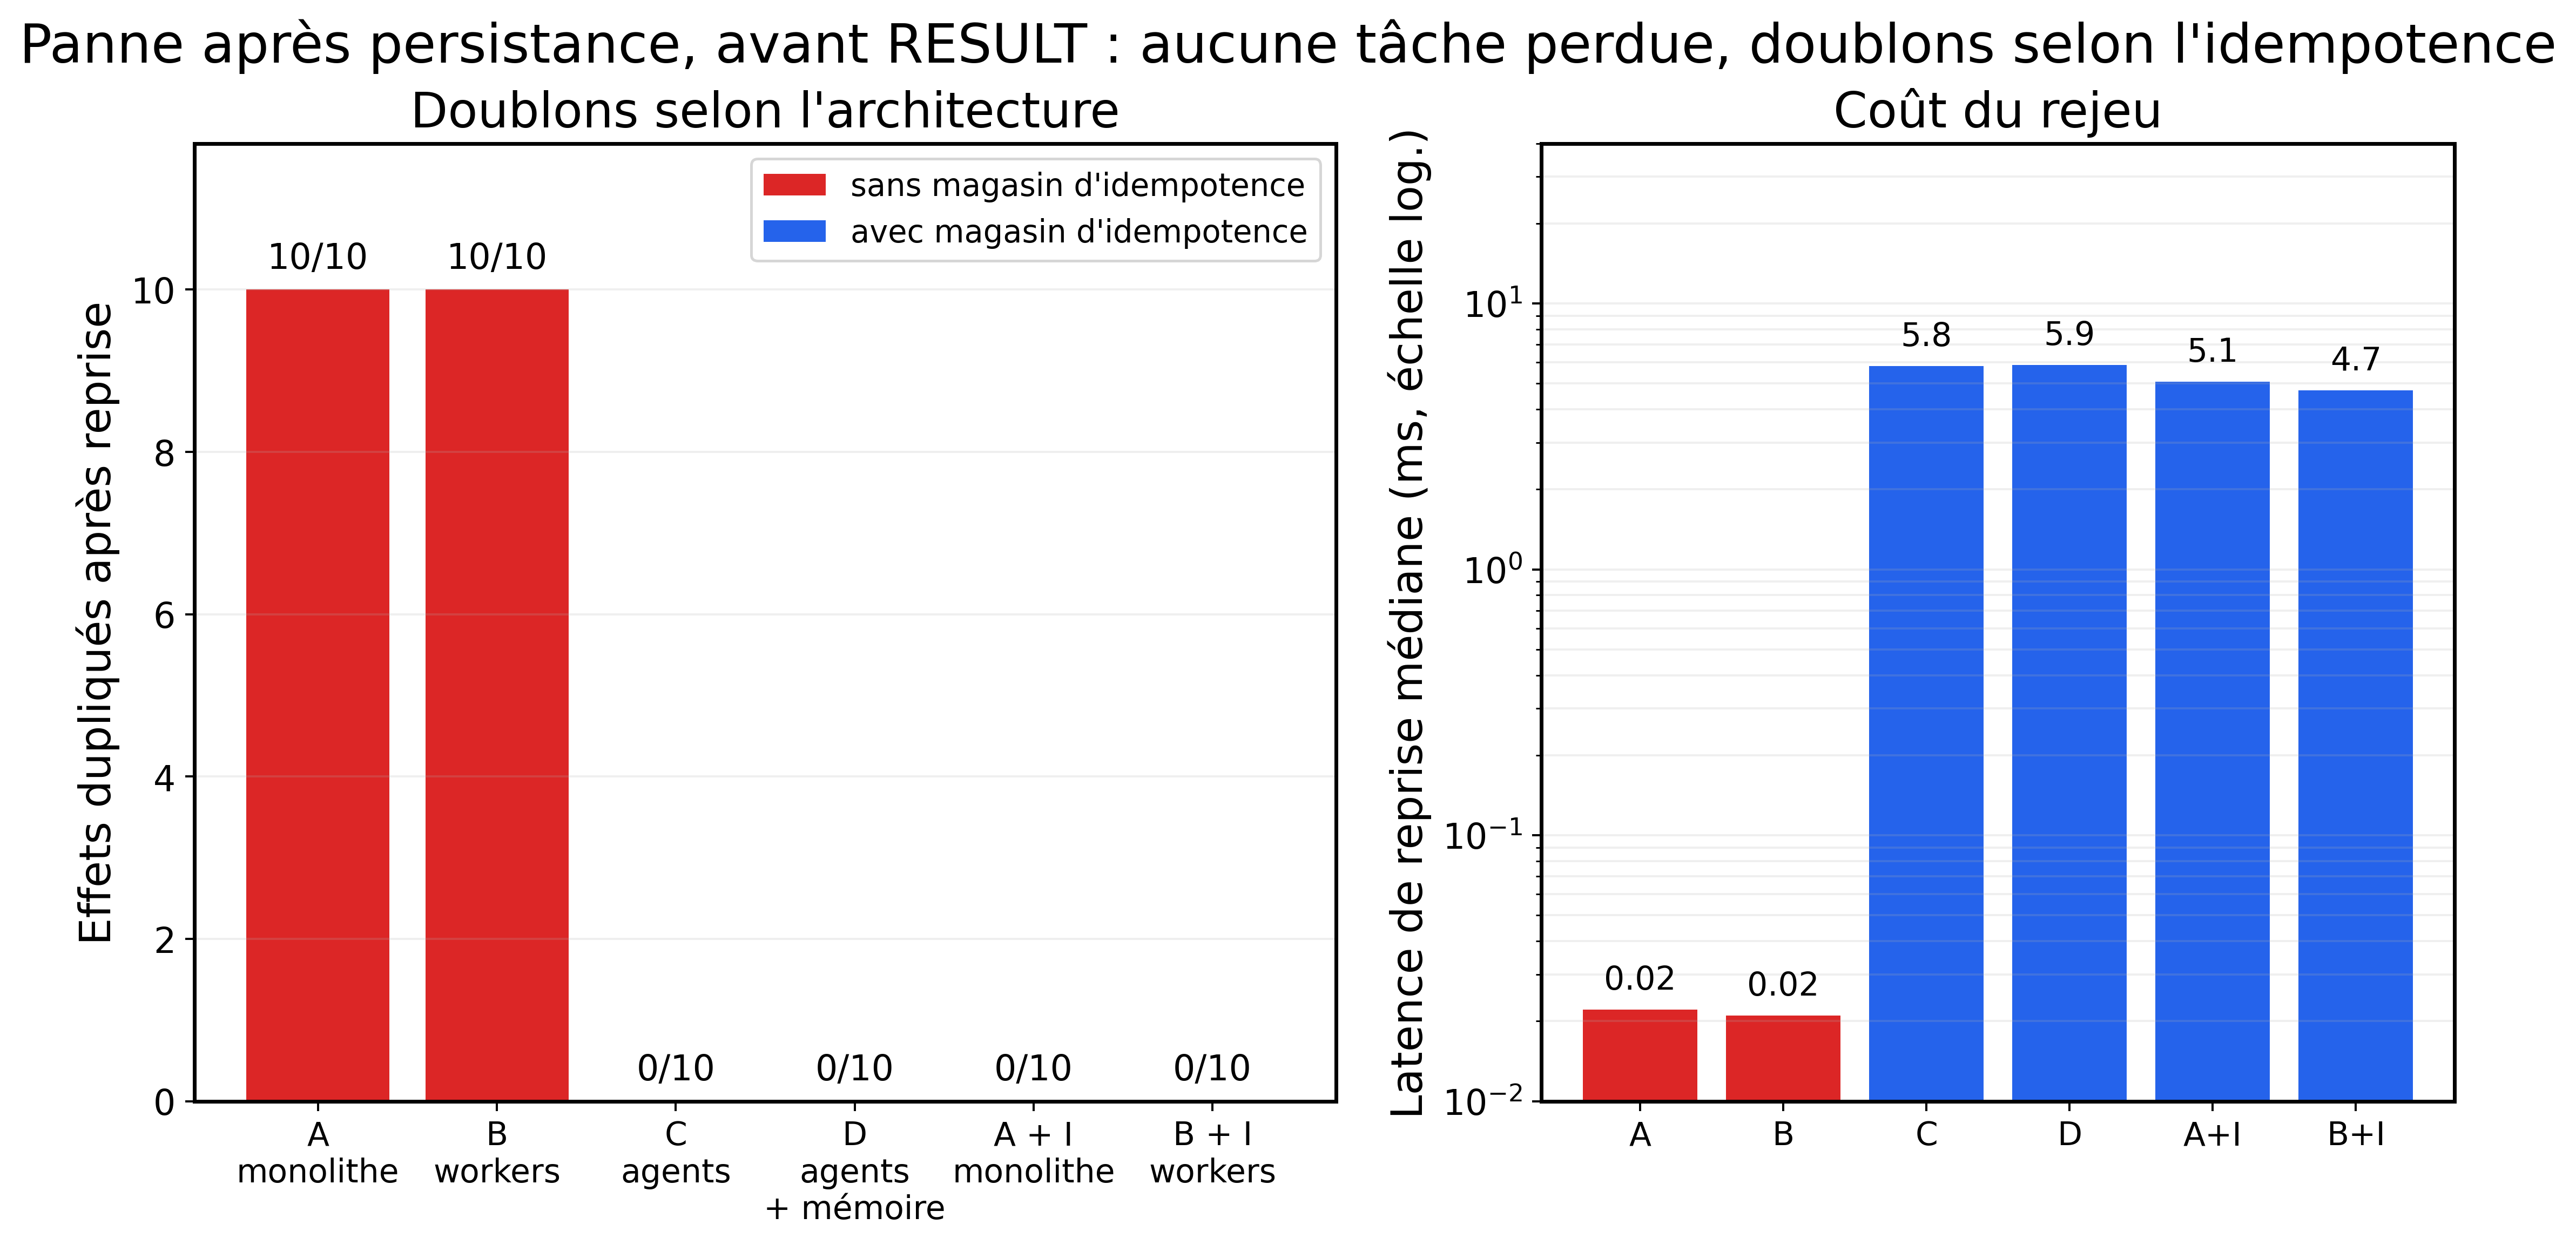
\includegraphics[width=0.98\textwidth]{fig_paired_failure_abcd.png}
  \caption[Panne appariée : doublons et coût du rejeu selon l'architecture.]{Effets dupliqués et latence de reprise médiane après une panne survenant entre la persistance et l'émission de \texttt{RESULT}, dix répétitions par architecture ; A\,+\,I et B\,+\,I désignent A et B dotés du magasin d'idempotence. Source : panne appariée A--D.}
  \label{fig:panne-appariee}
\end{figure}

\subsection{Mémoire sous fiabilité hétérogène}
\label{sec:e-h5}

Un protocole versionné avant son exécution compare C et D lorsque la fiabilité réelle des agents s'écarte de leur confiance déclarée. Pour chaque type de tâche, l'agent de plus forte confiance déclarée échoue avec une probabilité $p$, selon un tirage commun aux deux bras ; les autres agents ne reçoivent aucun échec. Les niveaux $0{,}3$, $0{,}6$ et $0{,}9$ ont été fixés pour couvrir un écart modéré, fort et extrême entre la confiance déclarée et la fiabilité réelle ; ils ne sont tirés d'aucune mesure opérationnelle. Chaque exécution porte sur $1\,000$ tâches synthétiques de 2~ms, avec trois coordinateurs concurrents et 30 graines. Le gain à un niveau exige que l'IC à 95~\% du delta du taux d'échec à la première exécution soit strictement négatif et que la borne inférieure de l'IC du rapport de débit atteigne au moins $0{,}95$.

\begin{table}[H]
\centering
\caption{Mémoire activée (D) contre désactivée (C) sous fiabilité hétérogène, 30 graines appariées.}
\label{tab:e-h5}
\footnotesize
\setlength{\tabcolsep}{4pt}
\begin{tabular}{lcccc}
\toprule
$p$ & \textbf{Échec initial C / D} & \textbf{Delta D $-$ C [IC 95~\%]} & \textbf{Débit D/C [IC 95~\%]} & \textbf{Gain} \\
\midrule
0,3 & 0,1096 / 0,1069 & $-0{,}0027$ [$-0{,}0086$ ; $0{,}0031$] & 0,972 [0,954 ; 0,991] & non \\
0,6 & 0,2405 / 0,2103 & $-0{,}0302$ [$-0{,}0389$ ; $-0{,}0215$] & 0,975 [0,942 ; 1,008] & non \\
0,9 & 0,3729 / 0,0736 & $-0{,}2993$ [$-0{,}3138$ ; $-0{,}2848$] & 1,210 [1,194 ; 1,225] & oui \\
\bottomrule
\end{tabular}
\end{table}

Selon la règle de décision, le gain est conditionnel : il n'est établi que pour $p = 0{,}9$, le niveau le plus éloigné d'une configuration réaliste. À $p = 0{,}6$, le taux d'échec diminue, mais le garde-fou de débit n'est pas satisfait ; à $p = 0{,}3$, l'intervalle contient zéro. Sur $30\,000$ tâches par niveau, les échecs finaux passent de 3 à 6, de 19 à 4 et de 44 à 3 entre C et D ; ces pertes relèvent du mécanisme de repli décrit en section~\ref{sec:e-cnp}. Même au niveau favorable, l'indice de Jain recule ($-0{,}037$ [$-0{,}041$ ; $-0{,}033$]).

L'analyse de sensibilité en exécution séquentielle, sur dix graines, ne participe pas à la décision. Elle montre un écart bien plus marqué : le taux de C reste voisin de $p$ ($0{,}303$ ; $0{,}602$ ; $0{,}901$), celui de D tombe à $0{,}033$, $0{,}006$ et $0{,}004$, tandis que l'indice de Jain baisse, selon le niveau, de $0{,}37$ à $0{,}41$. Sans concurrence, le terme de charge ne disperse plus les tâches : C reste sur l'agent défaillant et D se concentre sur un agent qui a réussi. Sous concurrence, l'étalement dû à la charge masque donc une grande partie de l'effet de la mémoire. L'expérience reste synthétique : échecs injectés, processus unique et confiance volontairement erronée. Elle concerne l'attribution entre agents, non la priorisation des anomalies, qui reste non mesurée.

\paragraph{Mémoire greffée sur un répartiteur centralisé.} Un contrôle décidé après la campagne précédente applique le même compteur lissé de Laplace à un répartiteur au moindre chargé. Il compare, sur 30 graines nouvelles et les mêmes trois niveaux, le répartiteur sans mémoire, sa version avec mémoire et D. Les tâches et les échecs potentiels sont appariés ; chaque exécution repart d'un état neuf. Le critère de gain est inchangé.

\begin{table}[H]
\centering
\caption{Mémoire activée ou non dans le répartiteur au moindre chargé, 30 graines appariées.}
\label{tab:e-h2-central}
\footnotesize
\setlength{\tabcolsep}{3pt}
\begin{tabularx}{\textwidth}{>{\centering\arraybackslash}p{0.7cm}>{\centering\arraybackslash}p{2.7cm}>{\centering\arraybackslash}X>{\centering\arraybackslash}p{3.0cm}>{\centering\arraybackslash}p{0.9cm}}
\toprule
$p$ & \textbf{Échec initial sans / avec} & \textbf{Delta avec $-$ sans [IC 95~\%]} & \textbf{Débit avec/sans [IC 95~\%]} & \textbf{Gain} \\
\midrule
0,3 & 0,1093 / 0,1055 & $-0{,}0038$ [$-0{,}0072$ ; $-0{,}0004$] & 0,987 [0,959 ; 1,015] & oui \\
0,6 & 0,2435 / 0,2191 & $-0{,}0243$ [$-0{,}0327$ ; $-0{,}0159$] & 1,024 [0,995 ; 1,053] & oui \\
0,9 & 0,3896 / 0,3496 & $-0{,}0400$ [$-0{,}0527$ ; $-0{,}0273$] & 1,010 [0,972 ; 1,049] & oui \\
\bottomrule
\end{tabularx}
\end{table}

Le gain est général selon la règle préenregistrée : les trois intervalles du delta sont strictement négatifs et les trois bornes inférieures du rapport de débit dépassent 0,95. Le contraste secondaire D contre le répartiteur sans mémoire n'est favorable qu'à $p=0{,}9$ ; la version centralisée avec mémoire ne surpasse D à aucun niveau. Le compteur lissé apporte donc aussi son effet sans négociation entre agents. Ce résultat soutient H2 pour le mécanisme de mémoire dans cette simulation, mais il relève de l'explication E2 : il ne permet d'attribuer le gain ni à Contract Net ni au caractère multi-agents. Il ne mesure pas davantage le coût d'un compteur partagé en environnement distribué.

\subsection{Contract Net face à une table statique}
\label{sec:e-cnp}

Un protocole versionné avant son exécution compare, sur les mêmes tâches et les mêmes agents, Contract Net sans mémoire (C), Contract Net avec mémoire (D) et une table statique. Celle-ci associe à chaque type de tâche la liste des agents par confiance déclarée décroissante, et passe à l'agent suivant en cas de refus ou d'échec. Elle exploite ainsi la même information déclarée, sans négociation, sans mémoire et sans observation de la charge. Le plan croise cinq scénarios, trois bras et 30 graines, pour $1\,000$ tâches par exécution et trois coordinateurs concurrents ; le scénario sans durée de service mesure le coût pur et n'entre pas dans la règle de décision.

\begin{table}[H]
\centering
\caption{Contract Net contre table statique, 30 graines appariées ; débits en tâches/s ; l'échec initial désigne l'échec à la première exécution.}
\label{tab:e-cnp}
\footnotesize
\setlength{\tabcolsep}{3pt}
\begin{tabularx}{\textwidth}{X>{\centering\arraybackslash}p{2.1cm}>{\centering\arraybackslash}p{3.0cm}>{\centering\arraybackslash}p{2.2cm}>{\centering\arraybackslash}p{1.9cm}}
\toprule
\textbf{Scénario} & \textbf{Débit table / C} & \textbf{C/table [IC 95~\%]} & \textbf{Échec initial table / C} & \textbf{Décision C / D} \\
\midrule
Coût pur, sans service & $13\,283$ / $2\,704$ & 0,211 [0,193 ; 0,229] & 0 / 0 & hors règle \\
Nominal, 2~ms & $1\,103$ / 956 & 0,867 [0,856 ; 0,878] & 0 / 0 & défav. / défav. \\
Fiabilité hétérogène, $p = 0{,}3$ & 856 / 865 & 1,011 [1,001 ; 1,020] & 0,2971 / 0,1095 & fav. / fav. \\
Panne silencieuse de \texttt{gamma} & 825 / 801 & 0,971 [0,964 ; 0,977] & 0,3500 / 0,2101 & fav. / fav. \\
\texttt{gamma} lent, 10~ms & 636 / 736 & 1,157 [1,149 ; 1,165] & 0 / 0 & fav. / indét. \\
\bottomrule
\end{tabularx}
\end{table}

La décision est un avantage conditionnel : favorable sur trois des quatre scénarios, défavorable en régime nominal. Contract Net échange environ dix messages par tâche. Il réduit le débit de 13\,\% lorsque le service dure 2~ms et ne conserve qu'un cinquième du débit de la table lorsque la tâche ne fait presque rien.

Ces gains ne proviennent pas d'une décision informée par les échecs : C n'a pas de mémoire et ignore ces derniers. Ils coïncident avec l'étalement produit par le terme de charge de l'utilité : en régime nominal, C répartit les exécutions à parts égales entre les trois agents, alors que la table en confie $49{,}3\,\%$ à \texttt{agent-gamma}. Comme les défaillances et la lenteur injectées visent les agents les plus sollicités par la table, s'en écarter suffit à les éviter. Le contraste C $-$ table ne sépare donc pas la négociation de la simple prise en compte de la charge ; la section~\ref{sec:e-cnp-moindre} teste ce point.

La table n'enregistre par ailleurs aucun échec final sur $30\,000$ tâches par scénario, alors que Contract Net perd quelques tâches lorsque des agents défaillent : 4 pour C et 8 pour D sous fiabilité hétérogène, 50 pour D sous panne silencieuse. Ces pertes n'apparaissent qu'avec plusieurs coordinateurs concurrents : en exécution séquentielle, aucune des $60\,000$ tâches de l'analyse de sensibilité de la section~\ref{sec:e-h5} n'est perdue, même lorsque l'agent préféré échoue neuf fois sur dix. Leur cause est dans la liste de repli. Elle est fixée au moment de l'appel d'offres et ne contient que les agents qui ont proposé ; or un agent occupé à cet instant refuse de proposer, et aucun nouvel appel d'offres n'est émis après un échec. La table statique et le répartiteur au moindre chargé, qui examinent tous les agents à chaque tentative, ne perdent aucune tâche. Ce défaut a été corrigé, et la comparaison reprise avec le coordinateur corrigé (section~\ref{sec:e-cnp-moindre}). Il s'agit d'un défaut de l'implémentation, non d'une propriété du protocole : une relance de l'appel d'offres après échec le corrigerait, mais elle n'a pas été testée. Que la mémoire, en concentrant les attributions, explique les 50 pertes de D sous panne silencieuse reste une hypothèse : les motifs de refus ne sont pas conservés.

\subsection{Contract Net face à un répartiteur au moindre chargé}
\label{sec:e-cnp-moindre}

Un protocole versionné avant son exécution, décidé après lecture de la comparaison précédente, sépare la négociation de la prise en compte de la charge. Un répartiteur choisit l'agent le moins occupé, avec la confiance déclarée en départage et le même repli, sans offre, sans mémoire et sans message de protocole. Les scénarios et la règle de décision sont inchangés ; les 30 graines sont nouvelles, soit 450 exécutions.

\begin{table}[H]
\centering
\caption{Contract Net sans mémoire (C) contre répartiteur au moindre chargé, 30 graines appariées ; débits en tâches/s.}
\label{tab:e-cnp-moindre}
\footnotesize
\setlength{\tabcolsep}{3pt}
\begin{tabularx}{\textwidth}{X>{\centering\arraybackslash}p{2.1cm}>{\centering\arraybackslash}p{3.0cm}>{\centering\arraybackslash}p{2.4cm}>{\centering\arraybackslash}p{1.7cm}}
\toprule
\textbf{Scénario} & \textbf{Débit répartiteur / C} & \textbf{C/répartiteur [IC 95~\%]} & \textbf{Échec initial répartiteur / C} & \textbf{Décision} \\
\midrule
Coût pur, sans service & $8\,402$ / $2\,598$ & 0,321 [0,298 ; 0,343] & 0 / 0 & hors règle \\
Nominal, 2~ms & $1\,098$ / 955 & 0,870 [0,857 ; 0,883] & 0 / 0 & défavorable \\
Fiabilité hétérogène, $p = 0{,}3$ & 962 / 824 & 0,859 [0,821 ; 0,897] & 0,1093 / 0,1094 & défavorable \\
Panne silencieuse de \texttt{gamma} & 882 / 783 & 0,890 [0,869 ; 0,912] & 0,2103 / 0,2099 & défavorable \\
\texttt{gamma} lent, 10~ms & 832 / 733 & 0,881 [0,868 ; 0,894] & 0 / 0 & défavorable \\
\bottomrule
\end{tabularx}
\end{table}

La décision est l'absence d'avantage : Contract Net est défavorable sur les quatre scénarios. Le répartiteur atteint les mêmes taux d'échec à la première exécution, les intervalles des deltas contenant zéro, et Contract Net perd 11 à 14\,\% de débit pour environ dix messages par tâche. Sur $30\,000$ tâches, le répartiteur ne perd aucune tâche sous fiabilité hétérogène, contre 5 pour Contract Net. Face à la table statique, le répartiteur est favorable sur les trois scénarios de charge inégale ou de défaillance et indéterminé en régime nominal (rapport de débit 0,991 [0,983 ; 1,000]). Sur ces nouvelles graines, C reste favorable face à la table lorsque \texttt{gamma} est lent et défavorable en régime nominal ; sous fiabilité hétérogène et panne silencieuse, il devient indéterminé, le garde-fou de débit n'étant plus satisfait (bornes inférieures 0,935 et 0,939). Les décisions favorables de la section~\ref{sec:e-cnp} sur ces deux scénarios ne sont donc pas stables d'un ensemble de graines à l'autre.

\paragraph{Tailles d'effet et réplication.} Une analyse secondaire, non préenregistrée, rapproche les deux jeux de 30 graines, qui contiennent tous deux le contraste C $-$ table. L'effet sur les échecs à la première exécution se réplique presque à l'identique : $-0{,}1877$ [$-0{,}1919$ ; $-0{,}1835$] puis $-0{,}1853$ [$-0{,}1899$ ; $-0{,}1807$] sous fiabilité hétérogène, $-0{,}1399$ puis $-0{,}1400$ sous panne silencieuse. Ce qui change d'un jeu à l'autre est le rapport de débit, dont la borne inférieure passe de $1{,}001$ à $0{,}935$ et de $0{,}964$ à $0{,}939$ : ces valeurs encadrent le seuil de $0{,}95$ du garde-fou. L'instabilité de la décision ne tient donc pas à l'effet sur les échecs, mais à un coût en débit situé au voisinage du seuil. Sur les 60 graines réunies, le rapport vaut $0{,}993$ [$0{,}972$ ; $1{,}014$] et $0{,}963$ [$0{,}954$ ; $0{,}971$]. Face au répartiteur, l'absence d'effet est informative : avec 30 graines, la plus petite différence d'échecs détectable avec une puissance de 80~\% est de $0{,}0064$ sous fiabilité hétérogène et de $0{,}0023$ sous panne silencieuse, et les intervalles observés, $[-0{,}0044 ; 0{,}0046]$ et $[-0{,}0021 ; 0{,}0012]$, excluent tout écart supérieur à un demi-point. Trente graines suffisent donc pour l'effet sur les échecs ; elles ne suffisent pas à trancher un rapport de débit proche de $0{,}95$.

\paragraph{Coordinateur à repli corrigé.} Le coordinateur comparé ci-dessus fixe sa liste de repli au premier appel d'offres, ce qui lui fait perdre des tâches. Une version corrigée émet un nouvel appel d'offres aux agents non encore tentés lorsque les offres en cours sont épuisées ; trois tests unitaires couvrent ce comportement, et l'ancien mode, conservé, reproduit sans écart l'ancien coordinateur. La comparaison au répartiteur a été reprise avec ce coordinateur, sous un protocole versionné avant son exécution, sur 30 nouvelles graines (450 exécutions). Contract Net ne perd plus aucune tâche, contre 5 auparavant, mais la décision est inchangée : il reste défavorable sur les quatre scénarios. Les deltas d'échec à la première exécution contiennent zéro ($0{,}0003$ [$-0{,}0029$ ; $0{,}0034$] sous fiabilité hétérogène, $-0{,}0003$ [$-0{,}0021$ ; $0{,}0015$] sous panne silencieuse), et le rapport de débit va de $0{,}848$ à $0{,}876$. L'absence d'avantage ne tenait donc pas au défaut de repli.

Cette comparaison avantage le répartiteur par construction. Il lit directement l'état de chaque agent dans la mémoire du processus, sans message, sans délai de transport et sans risque d'information périmée ; Contract Net, lui, fait transiter la même information par environ dix messages par tâche. Dans un système réparti, connaître la charge d'un agent distant a un coût et un retard, et l'écart mesuré ici pourrait se réduire ou s'inverser ; cette configuration n'a pas été testée, pas plus qu'une comparaison à Celery, à Kafka ou à un moteur de workflow. Les mêmes gains face à la table statique sont obtenus par le répartiteur seul : la prise en compte de la charge suffit à les expliquer. Dans le périmètre évalué, aucun résultat ne justifie le coût de la négociation, et rien n'établit qu'elle soit inutile hors de ce périmètre.

\section{Exécution de bout en bout avec modèles réels}

La campagne multi-source contient $1\,401$ unités : une unité Apache et 200 unités pour chacune des sept autres sources. La condition H suit une voie heuristique ; la condition M charge le modèle recommandé. M réalise $1\,400$ inférences réelles, utilise une voie de repli pour Apache et ne produit aucune erreur.

\begin{figure}[H]
  \centering
  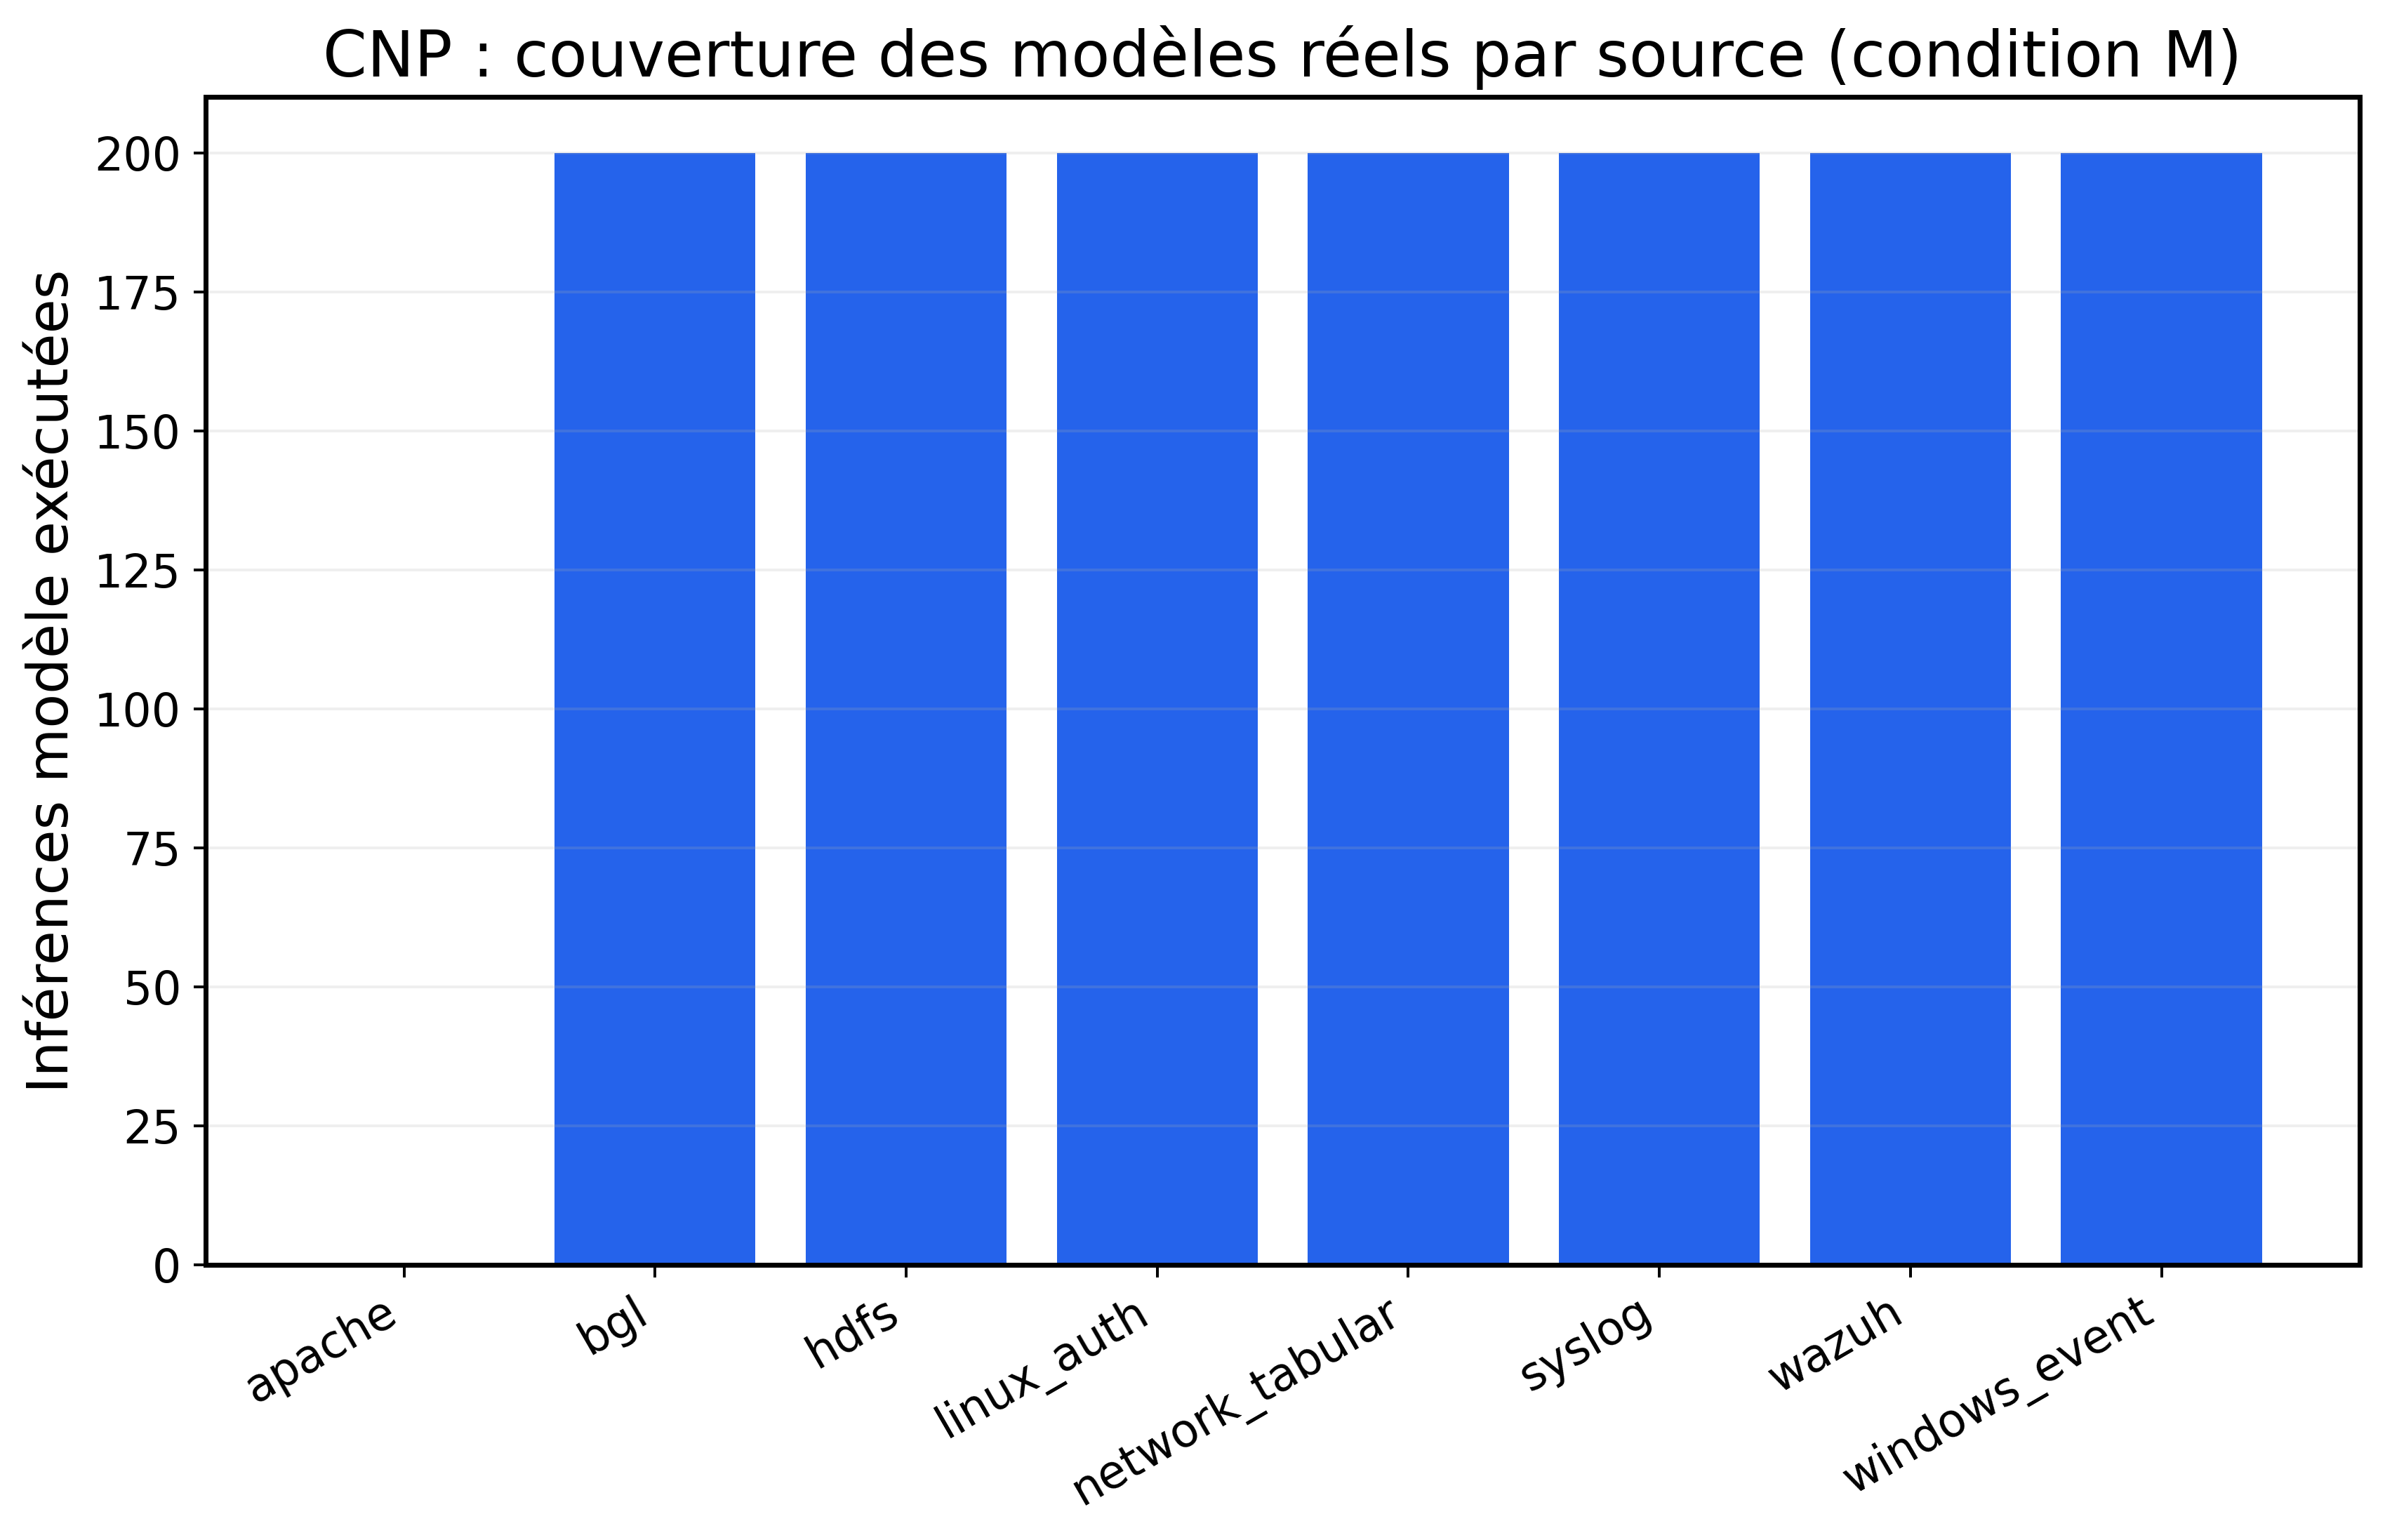
\includegraphics[width=0.97\textwidth]{fig_e2e_real_model_coverage.png}
  \caption[Couverture d’inférence de la condition M par source.]{Couverture d’inférence de la condition M par source. Source : exécution Contract Net multi-source.}
  \label{fig:e2e-couverture-modeles}
\end{figure}

La latence moyenne agrégée est $0{,}0310$~s pour H et $0{,}1054$~s pour M. Cette différence quantifie le coût du chargement et de l’inférence dans le protocole local.

\begin{figure}[H]
  \centering
  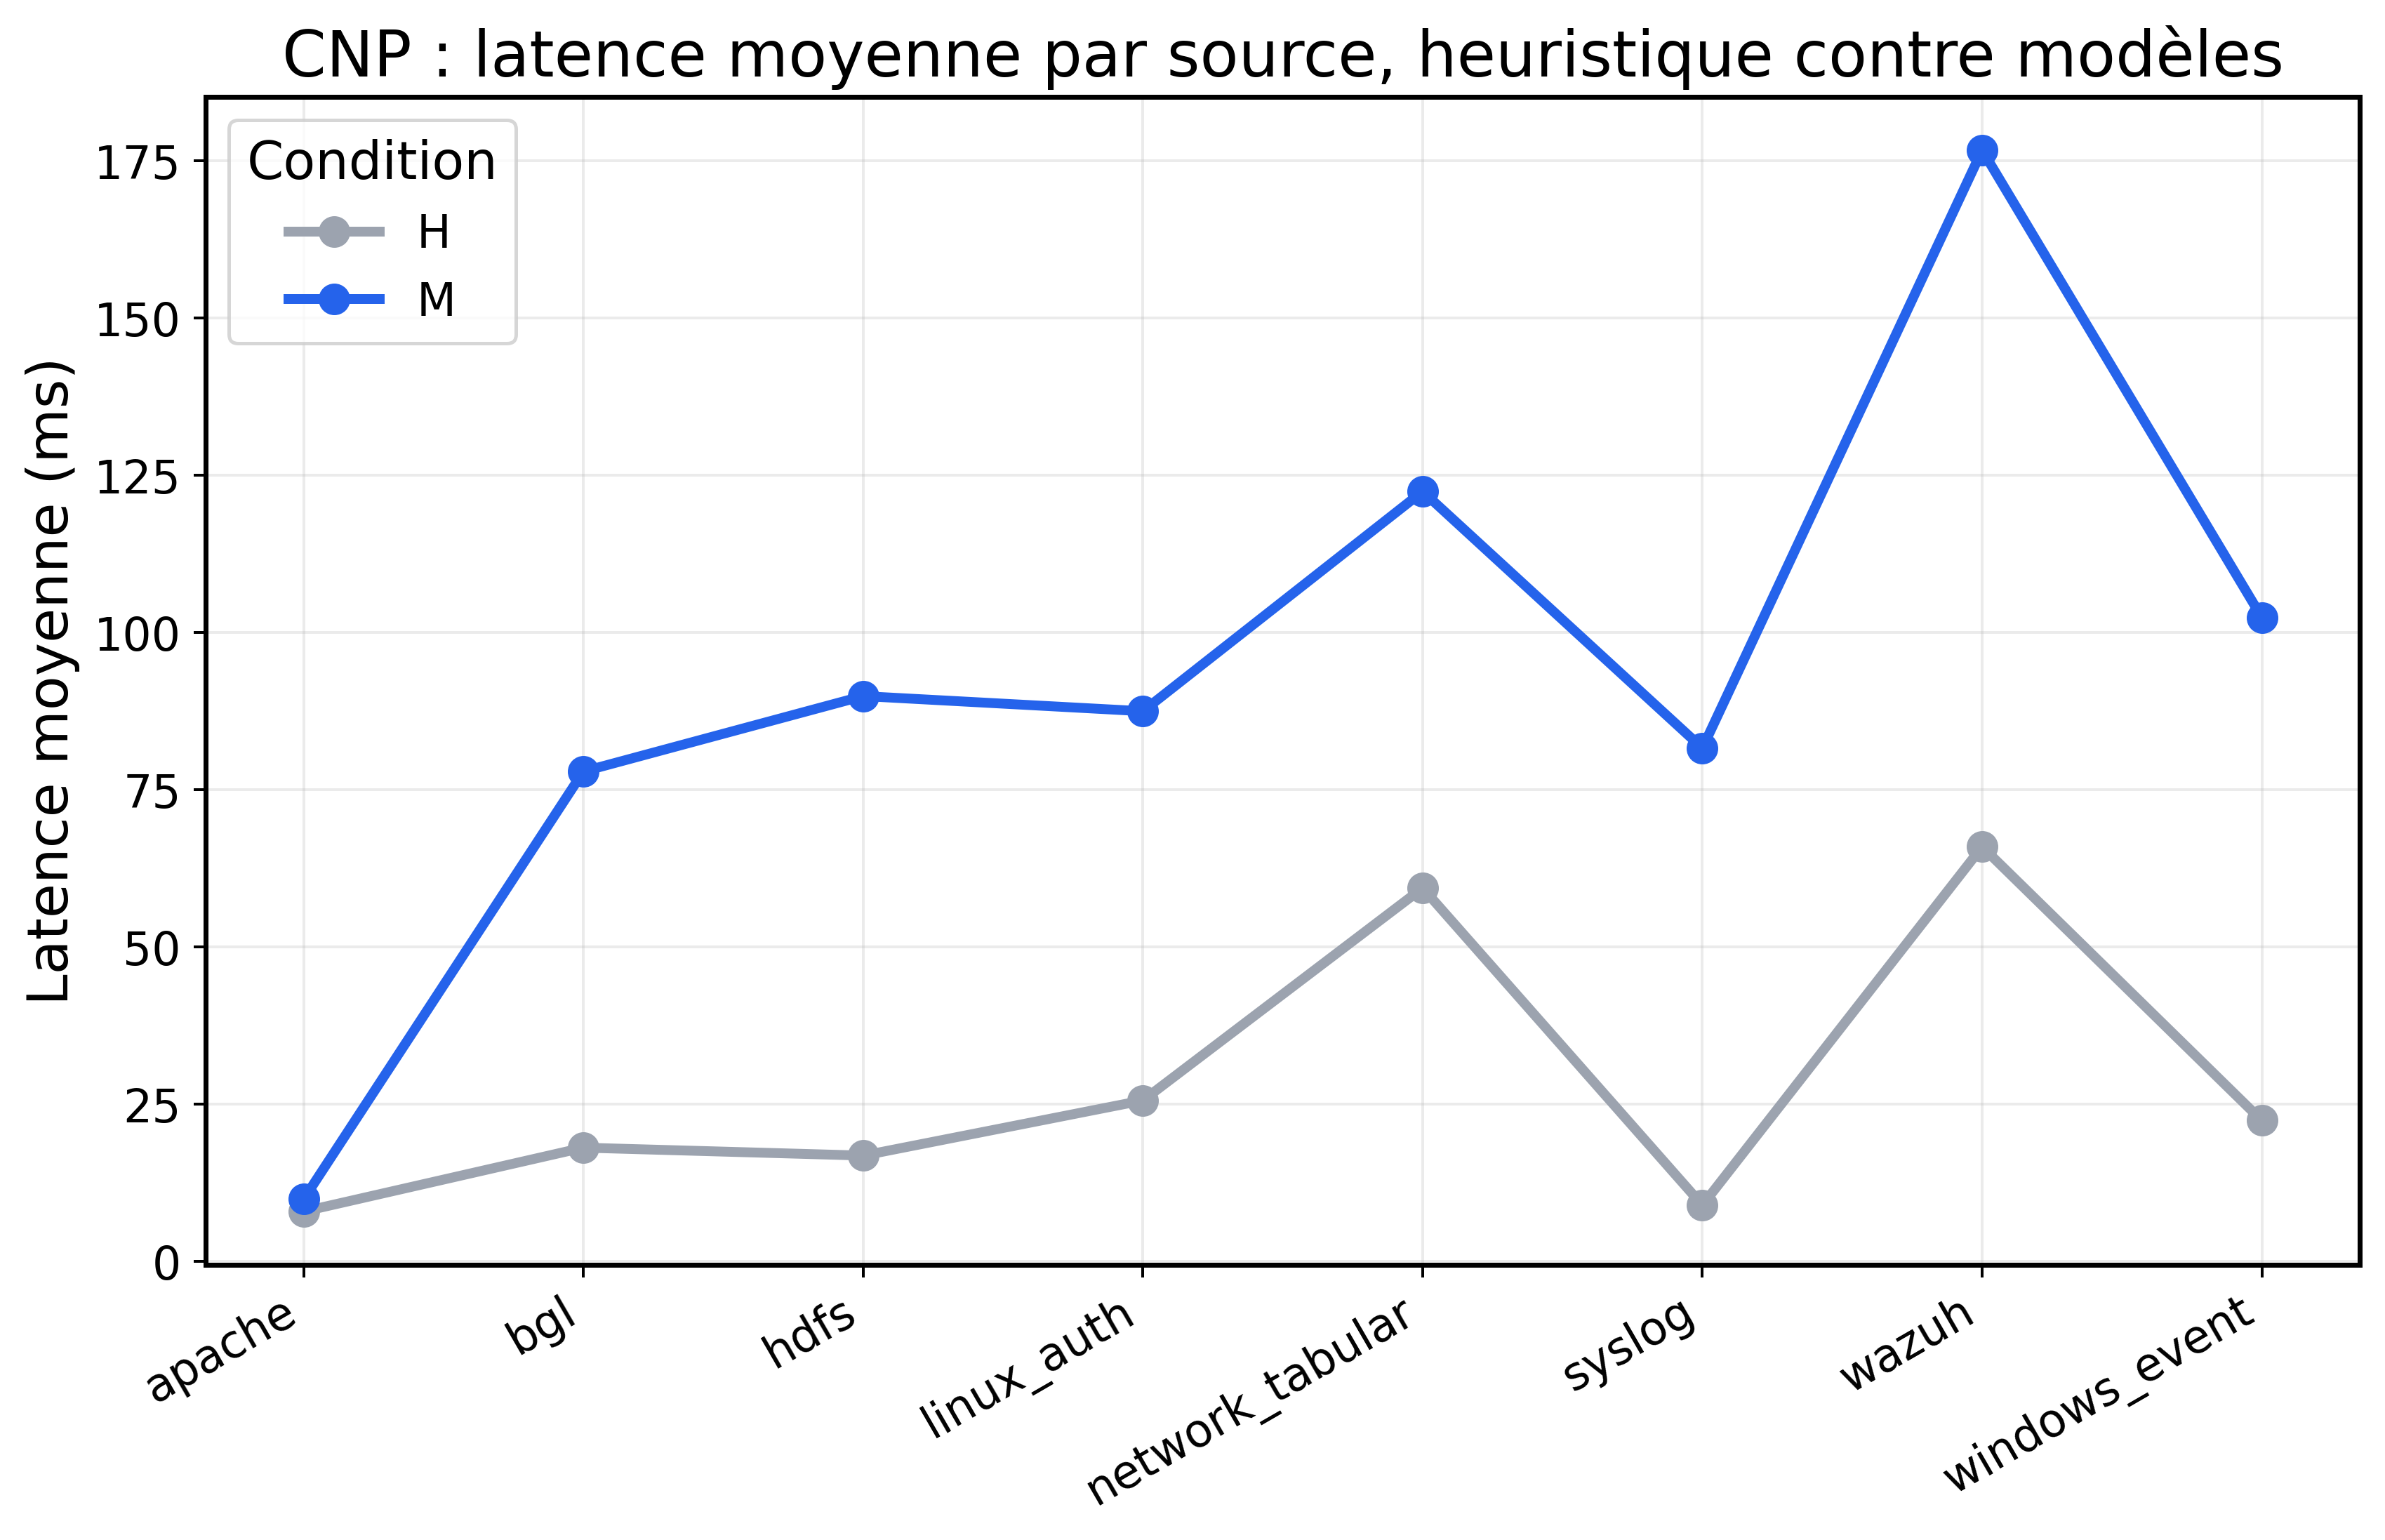
\includegraphics[width=0.98\textwidth]{fig_e2e_real_model_latency.png}
  \caption[Latence moyenne par source des conditions H et M.]{Latence moyenne par source des conditions heuristique H et modèles M. Source : exécution Contract Net multi-source.}
  \label{fig:e2e-latence-modeles}
\end{figure}

Les sources ne partageant pas une vérité terrain homogène, aucune exactitude globale n'est calculée. Le F1 de $0{,}3902$ observé sur Linux/auth, corpus synthétique, reste un résultat descriptif propre à cette source.

\section{Campagne Contract Net sur deux machines virtuelles}
\label{sec:cnp-multivm}

\subsection{Protocole}

Le coordinateur s’exécute sur l’hôte avec Redis 7.4.9 centralisé. Deux machines virtuelles participent : \texttt{debian-alpha} (Debian 13, Python 3.13.5) et \texttt{ubuntu-beta} (Ubuntu, Python 3.8.10). Chaque agent accepte au plus une tâche parallèle. La campagne d'endurance soumet une microtâche synthétique déterministe toutes les deux secondes pendant une heure, avec un point de reprise atomique toutes les cinq minutes. Cette charge cible la stabilité de l'orchestration ; elle ne mesure ni la qualité prédictive ni le coût d’une inférence réelle. Un scénario terminal force l’arrêt de l’agent Debian après persistance du résultat mais avant l’émission de \texttt{RESULT}, puis vérifie la réattribution et le rejeu idempotent.

\subsection{Endurance}

La durée observée atteint $3\,605{,}1$~s pour une cible de $3\,600$~s. Les $1\,800$ tâches planifiées se terminent toutes avec succès.

\begin{table}[H]
\centering
\caption{Résultats principaux de l'endurance d’une heure sur deux machines virtuelles.}
\label{tab:cnp-endurance}
\begin{tabularx}{0.92\textwidth}{p{0.42\textwidth} X}
\toprule
\textbf{Mesure} & \textbf{Observation} \\
\midrule
Durée cible / observée & $3\,600$ / $3\,605{,}1$ s \\
Tâches réussies & $1\,800/1\,800$ \\
Charge offerte (débit observé) & $0{,}4993$ tâche/s \\
Latence médiane / p95 / p99 & $53{,}98$ / $156{,}30$ / $836{,}73$ ms \\
Répartition & Debian : 451 ; Ubuntu : $1\,349$ \\
Reprise terminale & réattribution réussie ; rejeu idempotent \\
Effets persistants / dupliqués & 1 / 0 \\
\bottomrule
\end{tabularx}
\end{table}

Lors du scénario terminal, Debian persiste le résultat puis s’arrête avant de publier \texttt{RESULT}. Le coordinateur réattribue la tâche à Ubuntu ; le magasin Redis renvoie le résultat déjà persistant au lieu de répéter l’effet. Un seul effet est observé et aucun doublon n’apparaît. La répartition de 451 tâches pour Debian et $1\,349$ pour Ubuntu découle des profils de confiance configurés pour cette campagne, mémoire activée : le profil de Debian a la confiance la plus élevée pour l'analyse syntaxique ($0{,}95$ contre $0{,}78$, soit des premières offres de $0{,}86$ et $0{,}809$), celui d'Ubuntu pour le routage, la détection et la corrélation, et les quatre types de tâches sont soumis en rotation. La mémoire, qui ne s'enrichit que chez l'agent exécutant, accentue ensuite l'écart initial sans l'inverser. Debian remporte 450 tâches d'analyse syntaxique, Ubuntu 449 à 450 tâches de chacun des trois autres types ; les deux exceptions relèvent du scénario de panne.

\subsection{Saturation}

Un test de saturation en boucle ouverte soumet des tâches de décision HDFS à des débits croissants de 1 à 64 tâches/s, sur des fenêtres de 30~s répétées trois fois, avec 32 coordinateurs concurrents. Jusqu'à 8 tâches/s, le débit atteint suit la charge offerte et la latence médiane reste comprise entre $0{,}06$ et $0{,}22$~s. À partir de 16 tâches/s, le débit atteint plafonne entre $8{,}4$ et $15{,}0$ tâches/s et la latence p95 croît jusqu'à plus de 100~s, sous l'effet de l'attente côté coordinateur. Trois tâches sur $11\,430$ échouent par expiration de délai. L'agent Ubuntu ne reçoit des tâches qu'en saturation, lorsque l'agent Debian ne répond plus dans le délai imparti ; il remporte 143 attributions et en mène 140 à bien, soit $1{,}23\,\%$ des $11\,427$ tâches réussies, et les trois expirations le concernent toutes.

\paragraph{Origine du plafond.} Un diagnostic, versionné avant son exécution, a repris la saturation en trois configurations : les deux machines virtuelles, Debian seule, Ubuntu seule (débits offerts de 2 à 32 tâches/s, fenêtres de 20~s, trois répétitions). À 32 tâches/s, la capacité atteinte vaut $23{,}4$~tâches/s avec les deux machines et $24{,}4$ avec Debian seule : la seconde machine n'ajoute aucune capacité, et Ubuntu ne reçoit aucune tâche lorsque les deux agents sont présents. La cause tient au dispositif : chaque agent traite sa boîte de réception dans une seule boucle et n'exécute qu'une tâche à la fois ; les deux agents déclarent la même confiance, et le coordinateur départage les utilités égales par l'identifiant, ce qui attribue chaque tâche à Debian. Le plafond est donc la capacité d'un seul agent en série, et le dispositif ne pouvait pas montrer un partage de charge. Seule, Ubuntu plafonne à $14{,}9$~tâches/s, soit $0{,}61$ fois Debian ; cet écart ne peut pas être attribué à la seule version de Python (3.8.10 contre 3.13.5), les deux machines différant aussi par leur système et leurs ressources. Dans ce diagnostic, Debian atteint une capacité supérieure au plafond de 8,4 à 15,0~tâches/s mesuré plus haut ; cet écart n'est pas expliqué.

\begin{figure}[H]
  \centering
  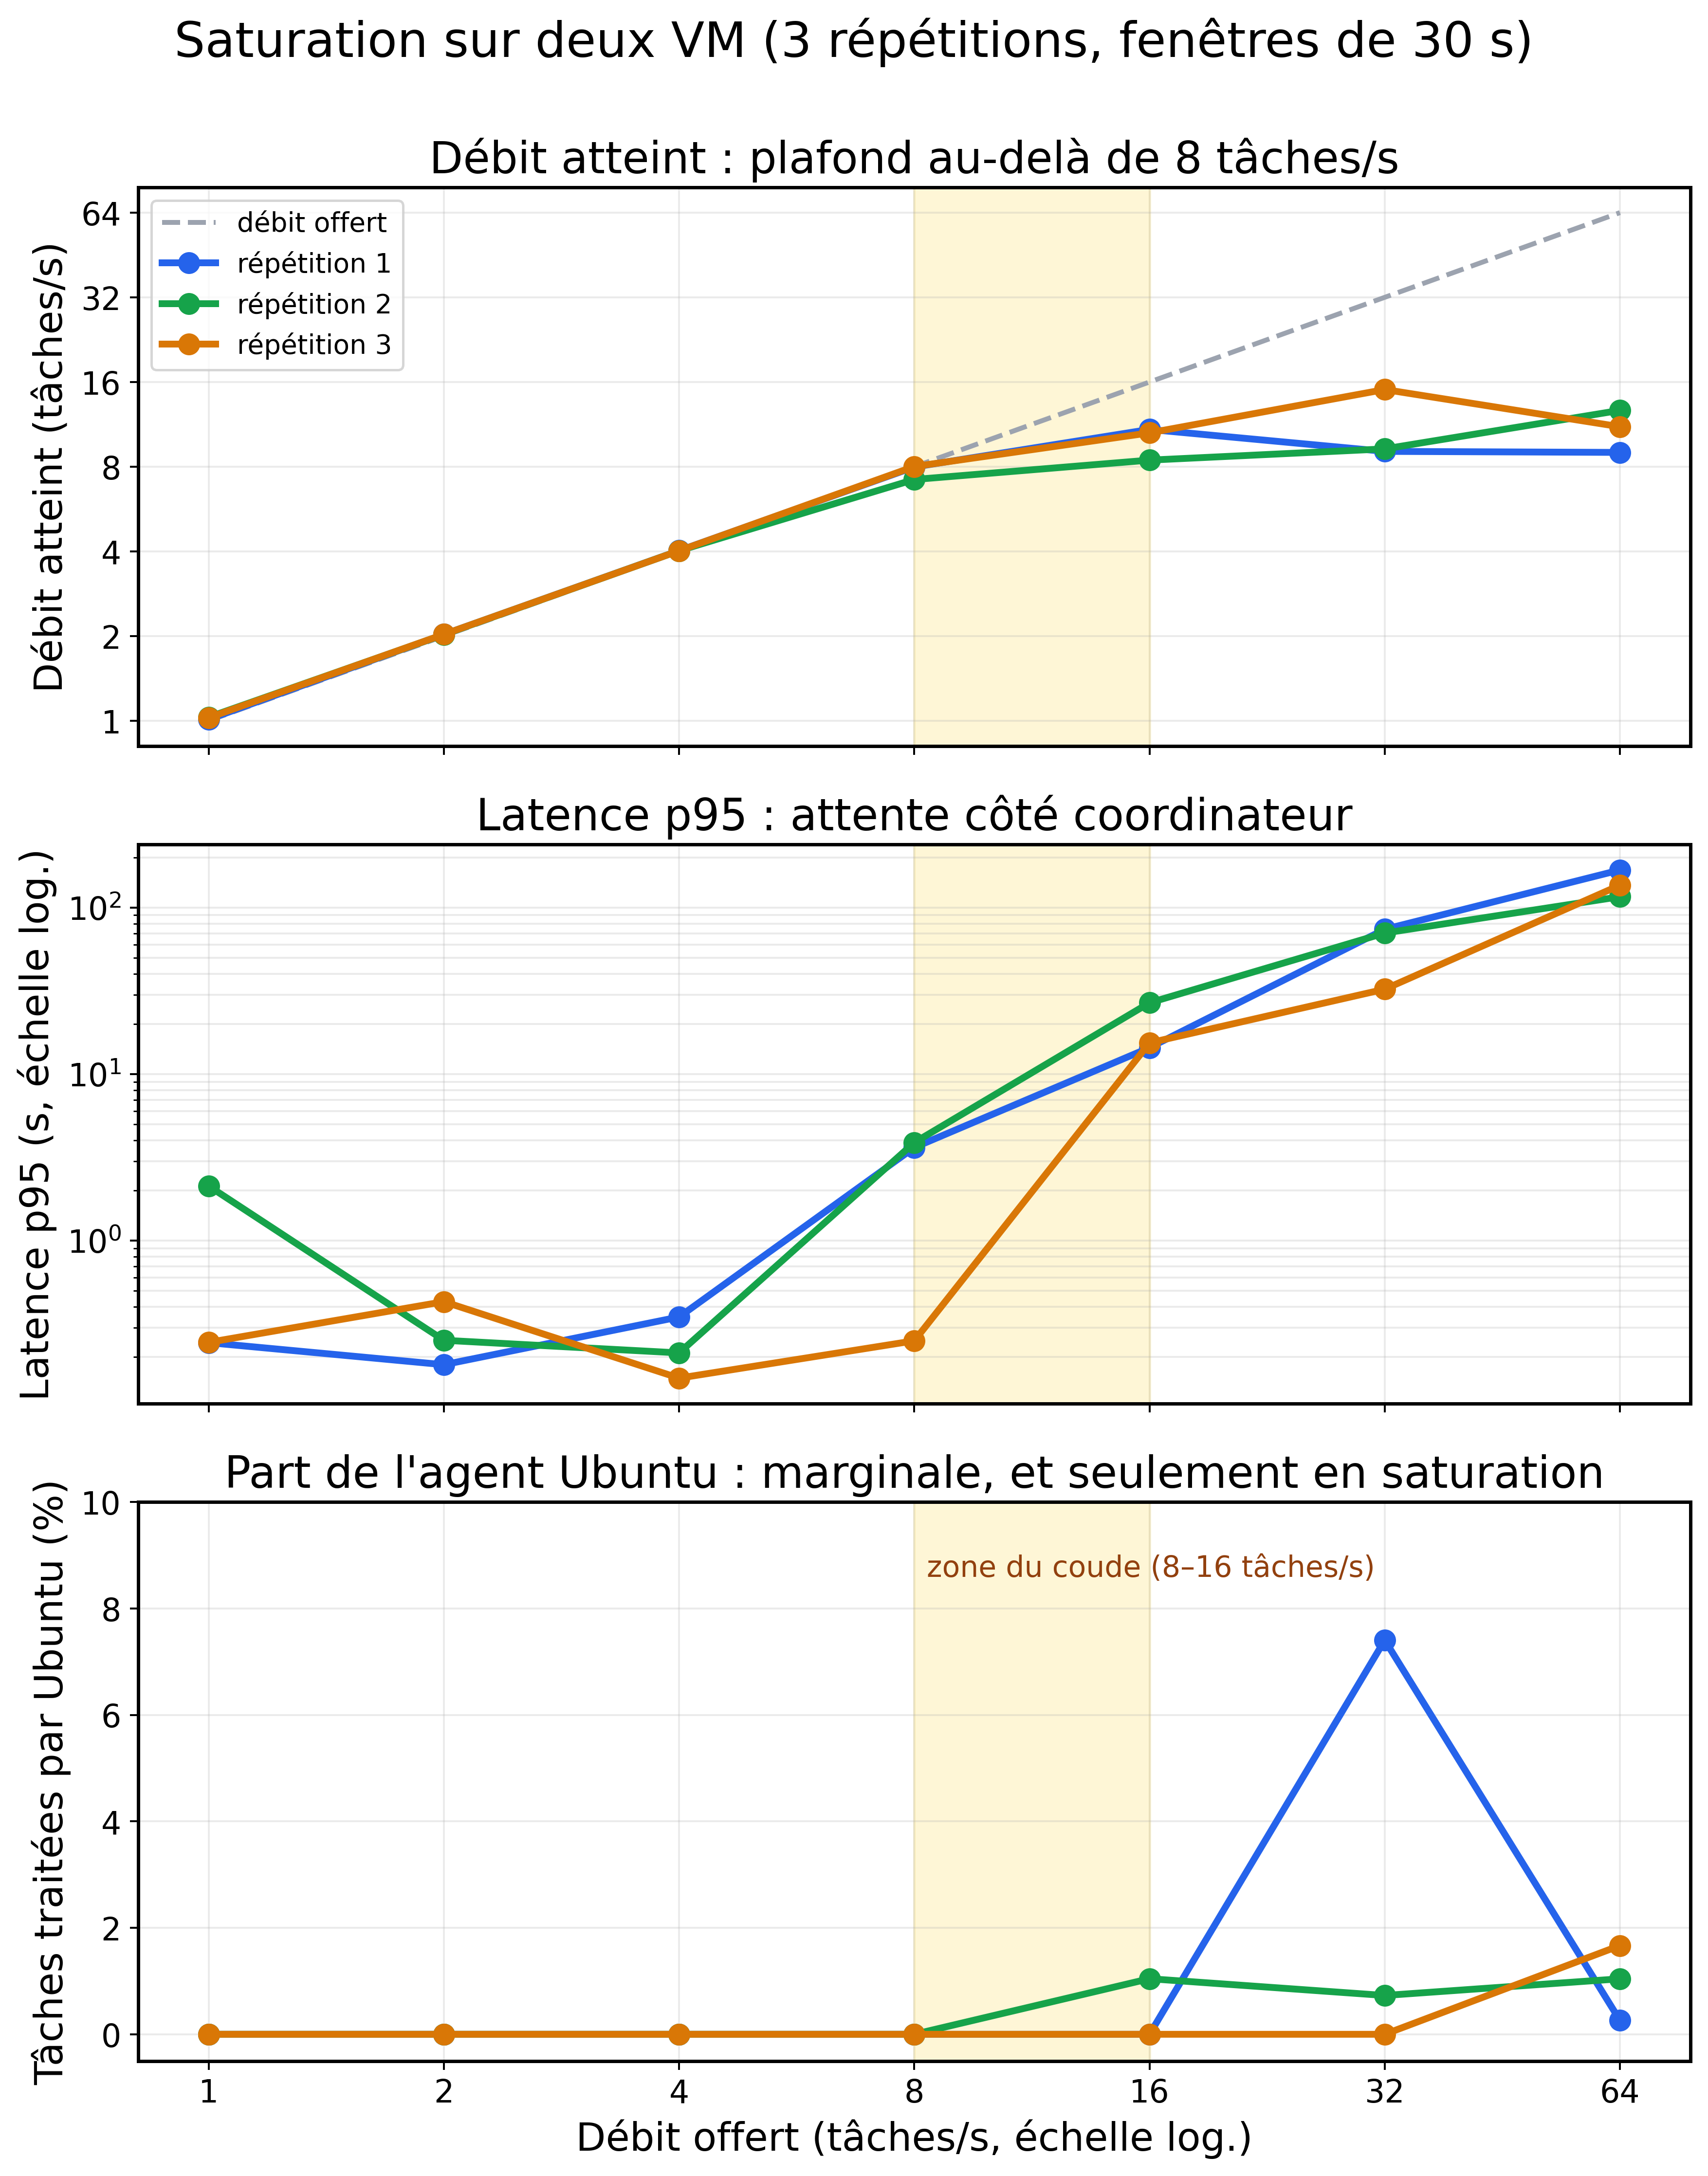
\includegraphics[width=0.80\textwidth]{fig_saturation_multivm.png}
  \caption[Saturation de la topologie à deux machines virtuelles.]{Débit atteint, latence p95 et part des tâches traitées par l'agent Ubuntu selon le débit offert, trois répétitions de 30~s par niveau. Source : saturation sur deux machines virtuelles.}
  \label{fig:saturation-multivm}
\end{figure}

\subsection{Détection HDFS répartie}
\label{sec:hdfs-distribue}

Un échantillon de $2\,000$ blocs du test HDFS, dont 29 positifs, passe par le Contract Net. Chaque tâche transporte l'identifiant du bloc, son étiquette et son score moyen calculé avec l'état Drain3 gelé ; l'agent attributaire applique le seuil figé $1{,}2729$ et renvoie sa prédiction. Les scores ne sont pas recalculés dans les machines virtuelles : l'expérience évalue la chaîne de décision distribuée, non un parsing distribué. Les $2\,000$ tâches aboutissent. La matrice de confusion vaut TP~$=29$, FP~$=7$, TN~$=1\,964$, FN~$=0$, soit un F1 de $0{,}8923$, identique au calcul centralisé sur les mêmes scores. La latence de négociation est de $57{,}69$~ms en médiane, $104{,}23$~ms au p95 et $236{,}23$~ms au p99, pour un débit de $14{,}92$ blocs/s en négociation séquentielle. Toutes les tâches sont attribuées à \texttt{debian-alpha}. Cette campagne n'emploie pas les profils de l'endurance : chaque agent déclare une seule capacité, de confiance $0{,}9$, pour l'unique type de tâche, et la mémoire est désactivée. Les deux agents proposent donc la même utilité ($0{,}845$, section~\ref{sec:spec-utilite}) et le coordinateur départage par ordre d'identifiant.

\subsection{Portée de la distribution}

La topologie à deux machines virtuelles démontre l'exécution répartie du protocole et la reprise idempotente entre hôtes, non un partage de charge ni une montée en capacité. En endurance, la charge offerte est très inférieure à la capacité, et la répartition découle des profils de confiance. En saturation, la seconde machine ne reçoit des tâches qu'une fois la première hors délai, et le plafond est atteint sans gain de capacité. En détection HDFS, toutes les tâches vont à un seul agent par départage. Les métriques par tâche, le résultat de reprise et le magasin d'idempotence sont complets ; les limites de cette validation, broker central compris, sont rassemblées à la section~\ref{sec:limites}.

\section{Corrélation d’incidents}
\label{sec:correlation-resultats}

Sur le corpus synthétique de référence (16 anomalies réparties en 6 incidents, soit 120 paires), le corrélateur réunit correctement 13 paires (TP), en réunit 4 à tort (FP) et en sépare 2 à tort (FN) : précision $13/17 = 0{,}7647$, rappel $13/15 = 0{,}8667$, F1 $0{,}8125$. Une baseline fondée sur la seule fenêtre temporelle obtient le même rappel avec 31 FP (précision $13/44 = 0{,}2955$).

Un générateur à graine produit en outre des corpus plus grands (20 graines, 80 incidents, 20 anomalies isolées et 40 événements non anomaux par corpus). Avec des clés stables, le corrélateur atteint, en comptes agrégés, $7\,076$ TP, 83 FP et $4\,770$ FN : précision $0{,}9884$ (intervalle bootstrap sur graines $[0{,}9808\,;\,0{,}9951]$) et rappel $0{,}5973$ ($[0{,}5837\,;\,0{,}6106]$). La fenêtre seule conserve le même rappel mais ne dépasse pas une précision de $0{,}2302$. Les omissions viennent de la fenêtre fixe, qui fragmente en moyenne 41 des 100 incidents vrais d’une graine ; ce total compte les 80 incidents et les 20 anomalies isolées, chacune formant un incident d'un seul événement. Lorsque 30\,\% des incidents enchaînent plusieurs catégories d’événements, le rappel tombe à $0{,}4835$ et la variante réduite à l’hôte et à la fenêtre obtient un meilleur F1 sur chacune des 20 graines ($0{,}7268$ contre $0{,}6496$). Les clés contextuelles apportent donc surtout de la précision ; elles fragmentent les incidents multi-étapes.

Ces corpus sont construits avec les clés mêmes qu'utilise le corrélateur : l'évaluation se fait en circuit fermé, et sa précision n'est pas transposable à des incidents réels (section~\ref{sec:limites}). Ces métriques décrivent uniquement la qualité du regroupement, distincte de celle de la détection en amont.

\section{Mise à jour contrôlée des modèles}

L’état de la gouvernance des modèles se lit par niveaux. Le code de comparaison existe et un mode d'essai à blanc calcule une décision sans remplacer le modèle actif. Certaines branches sont couvertes par des tests et plusieurs comparaisons ont été exécutées. Il manque une campagne complète où des candidats seraient successivement promus ou rejetés, puis évalués après mise à jour sur un jeu indépendant. Le statut retenu est donc : \textbf{IMPLÉMENTÉ} pour l’infrastructure de comparaison, \textbf{TESTÉ} pour les chemins couverts, \textbf{NON ÉVALUÉ} pour le bénéfice global et \textbf{PERSPECTIVE} pour une mise à jour autonome continue.

\section{Comparaison aux règles simples}
\label{sec:baselines-par-jeu}

Le tableau~\ref{tab:baselines-par-jeu} confronte, sous chaque protocole strict, le résultat principal à la meilleure règle simple évaluée sur le même test. La séparation aléatoire de CICIDS2017, qui dépasse la prédiction systématiquement positive, n'y figure pas, car elle ne mesure pas le transfert vers un scénario ou une période nouveaux.

\begin{table}[H]
\centering
\caption{Résultat principal et référence simple, par jeu et par protocole : F1, MCC et PR-AUC.}
\label{tab:baselines-par-jeu}
\small
\begin{tabularx}{\textwidth}{>{\raggedright\arraybackslash}p{0.2\textwidth} >{\raggedright\arraybackslash}X >{\raggedright\arraybackslash}p{0.15\textwidth} >{\raggedright\arraybackslash}p{0.27\textwidth}}
\toprule
\textbf{Jeu et protocole} & \textbf{Référence et statut} & \textbf{F1 réf. / modèle} & \textbf{MCC, PR-AUC du modèle} \\
\midrule
\multicolumn{4}{l}{\textit{Références fixées sans lecture du test}} \\
CICIDS2017, holdout par scénario & Tout positif ; critère préenregistré & 0,4737 / 0,2869 (SGD) & MCC moyen 0,11 à 0,18 selon le modèle (réf. 0), $\leq 0$ sur PortScan et Infiltration ; PR-AUC au-dessus de la prévalence dans les 25 cas \\
CICIDS2017, lundi--jeudi vers vendredi & Tout positif & 0,6667 / 0,5566 (LR) & MCC 0,436 (réf. 0) ; PR-AUC 0,871 (prévalence 0,5) \\
HDFS, test complet, niveau bloc & Surprise moyenne du template, apprise sur le normal (modèle léger ou règle) & 0,8724 / 0,8684 & MCC 0,874 (réf. 0,878) \\
HDFS, idem & Template jamais vu (règle triviale) & 0,0191 / 0,8684 & MCC 0,874 (réf. 0,093) \\
CSE-CIC-IDS2018, 16 vers 15 février & Tout positif ; port inférieur à 1024 & 0,095 ; 0,1215 / 0,2342 (LR) & MCC 0,229 (réf. 0,125) ; PR-AUC 0,141 (prévalence 0,050) \\
\midrule
\multicolumn{4}{l}{\textit{Références construites après lecture du test : exploratoires, hors de la preuve}} \\
BGL, niveau événement & Sévérité absente de l'entraînement & 0,9137 / 0,9137 & MCC 0,902 ; PR-AUC 0,841 (prévalence 0,145) \\
CSE-CIC-IDS2018, 15 vers 16 février & Port de destination inférieur à 1024 & 0,9997 / 0,9943 (LR) & MCC 0,987 ; sans le port : MCC 0,058 \\
\bottomrule
\end{tabularx}
\end{table}

Le critère préenregistré, le F1 face à la prédiction systématiquement positive sur le holdout par scénario de CICIDS2017, n'est atteint par aucun modèle ; pour ce jeu, le modèle indiqué est le meilleur des candidats, désigné après coup. Le MCC et la PR-AUC, ajoutés sans préenregistrement, nuancent cette lecture. Sur des tests équilibrés, le F1 de la prédiction systématiquement positive vaut $0{,}6667$ par construction et mesure surtout la prévalence ; en MCC comme en PR-AUC, les modèles dépassent la référence triviale, nettement sous séparation temporelle. Ils classent donc mieux que le hasard, mais leur seuil ne se transfère pas à une attaque absente de l'entraînement : sur PortScan et Infiltration, leur MCC est nul ou négatif. Sur HDFS, l'issue dépend du statut de la référence : la surprise moyenne des templates est apprise sur les blocs normaux avec un seuil calibré ; si on la tient pour un modèle léger, Histogram ne la dépasse pas, mais tous deux dépassent de loin la meilleure règle triviale. Les références de BGL et du transfert du 15 au 16 février dans CSE-CIC-IDS2018 ont été construites après lecture du test : elles éclairent la structure de ces tests sans servir de preuve. Dans le second cas, la régression logistique doit son score au port de destination ; sans cette variable, elle tombe au niveau de la prédiction systématiquement positive. Ces références ne sont pas des détecteurs recommandables ; elles fixent le niveau qu'un modèle doit dépasser pour que son score apporte une information. Les valeurs de MCC et de PR-AUC proviennent des artefacts des campagnes citées (annexe, tableau~\ref{tab:preuves-experimentales}).


% Chapitre 5
\chapter{Validité scientifique}
\label{chap:validite}

\section{Objet de l’analyse}

Les résultats présentés au chapitre précédent ne portent pas tous sur le même objet. Certains évaluent une performance prédictive, d’autres la reconnaissance d’un format, l’exécution distribuée ou encore la qualité de la corrélation. Ils ne se résument donc pas à une seule mesure.

Ce chapitre examine la solidité des conclusions selon quatre dimensions : validité interne, externe, de construit et statistique. L’objectif est moins de défendre chaque résultat que de préciser lesquels restent soutenus une fois leurs conditions d’obtention et leurs limites prises en compte.


\section{Validité interne}

La validité interne porte sur le lien entre le protocole expérimental et le résultat observé. Une difficulté majeure réside dans le risque de contamination entre les données utilisées pour préparer le modèle et celles destinées à son évaluation.

Dans HDFS, ce risque a été traité en séparant les blocs avant l’ajustement du parseur. Drain3 apprend 24 à 36 clusters selon la graine uniquement sur l’entraînement, puis fonctionne en mode \texttt{match\_only} sur la validation et le test. Le hash de son état reste identique avant et après l’inférence. L’agrégateur ainsi que le seuil sont, eux aussi, choisis à partir de la validation et non du test. Ces contrôles permettent d’écarter les formes de fuite explicitement instrumentées dans ce pipeline.

CICIDS2017 met en évidence un problème différent. Une partition aléatoire peut placer dans l’entraînement et le test des observations issues des mêmes scénarios. Dans ces conditions, le F1 de $0{,}9951$ reste correct pour la question posée par ce protocole, mais il ne décrit pas un transfert vers un scénario nouveau. Les holdouts par scénario et temporel répondent davantage à cette seconde question et produisent des performances nettement plus faibles.

Le cas de CSE-CIC-IDS2018 demande encore une autre lecture. La séparation par journée limite le mélange direct entre lignes d'entraînement et de test, mais elle n'empêche pas un raccourci propre à la journée de test. \texttt{Dst Port} utilisé seul atteint un F1 moyen de $0{,}9997$, et une règle fixe qui déclare attaque tout flux de port de destination inférieur à 1024 obtient le même score sur le 16 février, alors qu'elle n'atteint que $0{,}1215$ sur le 15 ; le transfert inverse, du 16 vers le 15 février, ne dépasse pas $0{,}2342$ (section~\ref{sec:csecic-raccourci}). La permutation des labels indique qu'aucune variable ne code directement le label, mais le score principal repose sur ce biais structurel entre les deux journées : la séparation par journée ne suffit donc pas à garantir que le modèle apprend une logique d'attaque transférable.

La comparaison des modèles communs et spécialisés illustre un autre risque. Une première exécution, pourtant préenregistrée et reproductible à l'identique, reposait sur un chargement qui incluait l'étiquette dans les variables d'UNSW et réduisait CICIDS aux attaques DDoS d'un seul fichier. Un rejeu ne révèle pas un tel défaut, puisqu'il le reproduit ; seule la lecture du code l'a mis en évidence (section~\ref{sec:e-h3b}). Les autres campagnes n'ont pas fait l'objet d'un audit de code aussi poussé.

Pour le routeur open-set, le seuil 100 est calibré uniquement à partir des sources connues. Après extension sans recalibration, les $20/20$ fichiers inconnus sont rejetés et $3/46$ fichiers connus le sont à tort. L’évaluation reste donc séparée de la calibration, mais les fichiers d'un même schéma ne sont pas indépendants et les faux rejets montrent la sensibilité aux variantes de schémas connus.


\section{Validité externe}

La validité externe concerne la possibilité d’étendre les observations à d’autres contextes que ceux effectivement testés.

Les datasets CICIDS2017 et CSE-CIC-IDS2018 reposent sur des scénarios construits et sur des caractéristiques de flux déjà extraites. Ils restent utiles pour comparer des protocoles dans un environnement contrôlé, mais leurs résultats ne peuvent pas être transférés automatiquement à d’autres capteurs, d’autres topologies ou d’autres périodes d’observation.

HDFS et BGL représentent eux aussi des contextes particuliers. Pour HDFS, l’évaluation finale porte sur les $115\,013$ blocs de test d'un seul système, dont $1\,679$ positifs. Les intervalles décrivent l'incertitude sur ce corpus ; ils ne décrivent pas une population universelle de systèmes distribués.

BGL présente une autre particularité : $89{,}8081\,\%$ des unités de test utilisent un template absent de l’entraînement. Une modification de ce taux de nouveauté pourrait donc changer sensiblement les performances observées.

La même prudence s’applique aux campagnes distribuées. Deux systèmes Linux participent à l’endurance avec un Redis central pendant $3\,605{,}1$~s et les $1\,800$ tâches planifiées réussissent. Une expérience de panne appariée, exécutée localement, montre séparément que l'idempotence évite l'effet dupliqué. Ces résultats ne renseignent pas sur les partitions réseau, le multi-site, un vieillissement sur plusieurs jours ou la haute disponibilité du broker.


\section{Validité de construit}

La validité de construit consiste à vérifier que la métrique employée représente bien la propriété annoncée.

Dans HDFS, la vérité terrain est définie au niveau du bloc. Le F1 calculé au niveau événement ne peut donc pas être considéré comme l’indicateur principal de la tâche. L’agrégation par \texttt{block\_id} est nécessaire pour aligner la prédiction sur l’unité des labels.

Pour BGL, un F1 global utilisé sans distinction entre templates connus et inconnus masquerait une partie importante du phénomène observé. La séparation de ces groupes permet de voir que la nouveauté lexicale participe fortement à la structure du test.

Le même principe vaut pour le routeur. La \texttt{decision\_margin} mesure un écart entre scores heuristiques ; elle ne représente pas une probabilité calibrée de bonne classification.

La couverture multi-format possède elle aussi une définition précise. Elle vérifie la lecture, le parsing et la normalisation des unités effectivement présentes dans la campagne. Elle ne mesure ni la conservation bit à bit du journal original, ni la complétude de tous les champs, ni la compatibilité avec toutes les implémentations possibles d’un format. La présence d’une seule fixture Apache doit donc rester visible dans l’interprétation.

Le caractère multi-agent ne se résume pas non plus au nombre de processus lancés. Dans ce travail, il est matérialisé par les capacités des agents, leur état local, la présence de plusieurs handlers et les comportements observés : proposition, refus, attribution, résultat ou échec. De la même manière, le replay idempotent montre qu’un effet logique instrumenté n’est pas dupliqué dans le scénario testé ; il ne transforme pas l’ensemble du système en transaction distribuée générale.

Dans les comparaisons de Contract Net, les défaillances et la lenteur sont injectées sur les agents que la table statique sollicite le plus. Un contraste favorable mesure donc l'évitement de ces agents, et non une qualité générale de la négociation ; c'est ce qui justifie la comparaison au moindre chargé.

Enfin, l’exécution effective d’un modèle et la qualité de sa prédiction sont deux propriétés distinctes. La campagne M établit que $1\,400$ inférences réelles sont réalisées sur $1\,401$ unités. Elle ne permet pas d’en déduire une exactitude globale, car les différentes sources ne partagent pas une vérité terrain homogène.


\section{Validité statistique}

La validité statistique dépend notamment du nombre de répétitions, de la variabilité observée et de l’unité choisie pour les calculs.

Les expériences CICIDS2017 et CSE-CIC-IDS2018 utilisent cinq graines. Le benchmark des architectures A--D répète quant à lui chaque combinaison dix fois. Ces répétitions rendent la dispersion observable, sans couvrir pour autant toutes les variations possibles des scénarios.

Cette limite est particulièrement visible dans les holdouts CICIDS2017. Leur écart-type élevé traduit des différences importantes de difficulté entre les attaques laissées hors entraînement. La moyenne doit donc être lue avec cette hétérogénéité.

Sur HDFS, les intervalles sont calculés au niveau \texttt{block\_id}, c’est-à-dire à l’unité utilisée par l’évaluation : intervalles exacts pour la précision, le rappel et le FPR, puis bootstrap multinomial de $20\,000$ réplications pour le F1 et le MCC. Ils ne corrigent cependant pas un éventuel biais de sélection du corpus.

BGL présente une difficulté différente : aucun positif n’est présent dans le groupe des templates connus. Il est donc impossible d’y calculer un rappel d’anomalies connues.

Le benchmark multi-agent porte enfin sur des micro-tâches. Dans ce contexte, le monolithe profite d’un coût de coordination très faible, alors que le Contract Net exige plusieurs échanges pour une même attribution. Des tâches plus lourdes pourraient modifier ce compromis, mais cette possibilité relève d’une hypothèse à tester. Les comparaisons préenregistrées utilisent 30 graines et des tâches de 2 à 10~ms : elles établissent que, dans un seul processus, la négociation n'apporte aucun avantage sur une répartition au moindre chargé. Elles ne couvrent ni les tâches plus lourdes ni l'exécution distribuée.


\section{Risques résiduels et mesures de contrôle}

Le tableau~\ref{tab:risques-validite} rassemble les principaux risques qui demeurent après les contrôles réalisés.

\begin{table}[H]

\centering

\caption{Principaux risques résiduels après consolidation.}

\label{tab:risques-validite}

\small

\begin{tabularx}{\textwidth}{p{0.22\textwidth} p{0.31\textwidth} X}

\toprule

\textbf{Risque} & \textbf{Contrôle réalisé} & \textbf{Limite restante} \\

\midrule

Proximité train/test & Splits scénario, temporel et par bloc & Datasets publics et scénarios limités. \\

Parsing contaminé & Drain3 ajusté sur l'entraînement, état gelé & Vérifié pour le pipeline HDFS étudié. \\

Nouveauté lexicale BGL & Groupes connu/inconnu et baseline & Aucun positif dans le groupe connu. \\

Dépendance aux variables & Mono-features, coefficients, ablation, permutation & Biais journalier toujours possible. \\

Surajustement du rejet & Calibration sur connus seulement ; extension à 20 inconnus sans recalibration & Faux rejets sur variantes de schémas connues ($3/46$). \\

Confusion distribution/HA & Deux VM et Redis central explicités & Broker et partitions non testés. \\

Confusion mémoire/gain & Comparaison ON/OFF, fiabilité hétérogène & Gain établi seulement à $p = 0{,}9$. \\

Confusion négociation/charge & Comparaison à un répartiteur au moindre chargé & Un seul processus ; exécution distribuée non testée. \\

\bottomrule

\end{tabularx}

\end{table}


\section{Conclusions soutenues}

Après ces contrôles, plusieurs conclusions restent directement soutenues par les expériences.

Le prototype parvient à lire, parser et normaliser les unités prévues dans la campagne multi-format. Avec le seuil gelé, le routeur rejette les $20/20$ fichiers inconnus du corpus étendu, tandis que $3/46$ fichiers connus sont rejetés à tort ; les 43 connus acceptés sont correctement orientés. Dans la campagne utilisant les modèles réels, $1\,400$ unités sur $1\,401$ passent effectivement par une inférence.

Le comportement des agents est également observable au-delà d’une simple description architecturale. Dans la campagne d'endurance multi-VM, ils proposent pour les tâches, les exécutent, produisent des résultats et participent à une réattribution après l'échec contrôlé. Le replay instrumenté ne produit pas de second effet persistant.

Ces résultats permettent de soutenir le fonctionnement du prototype dans les conditions expérimentales décrites. Ils ne suffisent cependant pas à conclure à une exactitude globale sur des sources hétérogènes, à une supériorité générale du routage spécialisé, à un bénéfice propre de la négociation, à un bénéfice général de la mémoire, à une mise à jour autonome des modèles ou à une disponibilité industrielle.

\section{Limites du travail}
\label{sec:limites}

Cette section est la seule qui rassemble les limites du travail ; les autres chapitres y
renvoient sans les reprendre.

\paragraph{Données et généralisation.}
CICIDS2017 repose sur des scénarios construits et sur des caractéristiques de flux déjà
extraites ; les CSV d'origine sont employés, sans les corrections publiées
\cite{engelen2021troubleshooting,lanvin2023errors}. Le score dépend fortement du
protocole : le même Random Forest passe de $0{,}9951$ en séparation aléatoire à $0{,}4374$
en séparation temporelle. Dans la campagne d'origine du holdout par scénario,
l'échantillonnage retenait les premières lignes du premier fichier lu, si bien que
l'entraînement ne couvrait qu'un seul scénario d'attaque ; cette campagne a été corrigée et
réexécutée, et ses anciens chiffres ne sont plus utilisés. Après correction, aucun des cinq
modèles évalués ne dépasse la prédiction systématiquement positive
(section~\ref{sec:cicids-resultats}). La provenance des deux fichiers CSE-CIC-IDS2018 a été
vérifiée par un nouveau téléchargement depuis la source : leurs empreintes coïncident avec
les copies utilisées par les campagnes. Seules les journées des 15 et 16 février sont
cependant évaluées, et les fichiers s'arrêtent à une limite de lignes compatible avec une
exportation par tableur. Le score du 15 vers le 16 repose sur le port de destination et ne
se transfère pas dans le sens inverse (section~\ref{sec:csecic-resultats}). Le corpus
Linux/auth est un jeu public entièrement synthétique, généré avec la bibliothèque Faker et
diffusé sur Kaggle ; ses variables \texttt{status} et \texttt{service} peuvent servir de
mandataires de l'étiquette. Aucun résultat obtenu sur Linux/auth ne vaut pour des journaux
d'authentification réels. Aucun de ces résultats ne se transpose sans nouvelle évaluation à
d'autres capteurs, topologies ou périodes d'observation.

\paragraph{Corpus et incertitude.}
Le test HDFS couvre les $115\,013$ blocs de la partition finale, dont $1\,679$ positifs.
L'intervalle bootstrap du F1, $[0{,}8568\,;\,0{,}8795]$, décrit l'incertitude sur ce corpus
d'un seul système, non sur une population de systèmes distribués. Les cinq graines ne
modifient que l'échantillon d'ajustement du parseur et donnent la même matrice de
confusion : elles constituent une seule observation du test. La sensibilité du résultat à la
taille de cet échantillon, $6\,000$ blocs, n'a pas été évaluée, et la prévalence plus faible
du test ($1{,}46\,\%$ contre $3{,}48\,\%$ en validation) abaisse mécaniquement la précision
au seuil choisi en validation. Sur BGL, le groupe des templates connus ne contient aucune
anomalie et $89{,}81\,\%$ du test relève d'un template inconnu de l'entraînement ;
Histogram y applique exactement la règle « sévérité absente de l'entraînement ». Les
variantes de protocole BGL, dont l'une a été conçue après lecture du test, sont
exploratoires et ne remplacent pas le protocole principal.

\paragraph{Routage et normalisation.}
La politique open-set rejette $20/20$ fichiers inconnus mais écarte aussi $3/46$ fichiers
connus. Ses scores reprennent pour les journaux texte les colonnes \texttt{dataset} et
\texttt{subtype} du parseur de format : le rejet mesure donc en partie la capacité du
parseur à ne pas reconnaître un format. Sa calibration ne repose que sur trois fichiers
inconnus, les fichiers d'un même schéma ne sont pas indépendants et la
\texttt{decision\_margin} n'est pas une probabilité calibrée. La comparaison à une chaîne
sans routage n'a pas été exécutée ; H3 reste non tranchée. La couverture multi-format mesure
la lecture, le parsing et l'émission des unités présentes ; la voie Apache repose sur une
seule fixture, et les flux réseau tabulaires ne renseignent aucun des sept champs standard
mesurés.

\paragraph{Grandeurs non mesurées.}
Les sources ne partagent pas de vérité terrain homogène : aucune exactitude globale n'est
calculée. Aucune expérience n'analyse conjointement un même incident à partir de journaux
système et de flux réseau ; l'hétérogénéité étudiée est celle des formats, lus séparément.
La corrélation est évaluée en circuit fermé, sur des corpus synthétiques construits avec les
clés mêmes du corrélateur. L'utilisabilité du tableau de bord, le temps d'investigation et
la charge cognitive n'ont fait l'objet d'aucune étude auprès d'analystes. La priorisation
des anomalies, les traitements périodiques et l'exécution par micro-lots ne sont pas
évalués. Le budget local de temps et de mémoire associé à H4 n'a jamais été fixé, et il ne
l'est pas après coup.

\paragraph{Distribution et exploitation.}
La validation distribuée porte sur deux machines virtuelles et un Redis central. La
campagne d'endurance offre environ $0{,}5$ tâche par seconde, loin de la capacité, et la
répartition de ses tâches suit les profils de confiance déclarés. En saturation, le coude se
situe entre 8 et 16 tâches/s, avec trois expirations de délai sur $11\,430$ tâches, et la
seconde machine ne traite que $1{,}23\,\%$ des tâches réussies : la distribution est
fonctionnelle, mais elle n'accroît pas la capacité observée. Dans la détection HDFS
répartie, les utilités égales sont départagées par un ordre fixe et toutes les tâches vont
au même agent ; l'inférence n'y est pas recalculée sur les machines virtuelles. La trace de
messages de l'endurance est tronquée à $10\,001$ événements, ce qui rend ses compteurs non
conclusifs. Ni panne du broker, ni partition réseau, ni fonctionnement multi-site, ni
vieillissement sur plusieurs jours ne sont testés. TLS, contrôle d'accès, gestion des
secrets, journalisation protégée, réplication, sauvegarde et observabilité distribuée ne
sont pas évalués.

\paragraph{Mécanismes adaptatifs.}
La fonction d'utilité est un classement à poids fixes, non appris
(section~\ref{sec:spec-utilite}). La mémoire n'apporte de gain qu'à une probabilité d'échec
de $0{,}9$, avec une équité moindre, dans un protocole où la confiance déclarée est
volontairement éloignée de la fiabilité réelle (section~\ref{sec:e-h5}). Contract Net
n'obtient aucun avantage sur un répartiteur au moindre chargé
(section~\ref{sec:e-cnp-moindre}) ; ce répartiteur lit l'état des agents dans un seul
processus, sans coût de communication ni information périmée, et la comparaison n'a pas été
reprise en exécution distribuée. Sous Contract Net, quelques tâches sont perdues, parce que
la liste de repli est figée au moment de l'appel d'offres. Dans la panne appariée, l'absence
de doublon provient du magasin d'idempotence, qui l'évite aussi lorsqu'il est ajouté aux
architectures de référence. La mise à jour contrôlée des modèles dispose d'un mode
\textit{dry-run}, mais d'aucun cycle complet et répété de promotion et de rejet
(tableau~\ref{tab:statut-model-update}).

\paragraph{Statut du système.}
Ariel \logminer{} est un prototype de laboratoire. Il ne constitue ni une plateforme
opérationnelle de SOC ni un système autonome prêt pour la production.



% Chapitre 6
\chapter{Discussion générale}

\section{Ce qui est implémenté, testé et effectivement supérieur}
\label{sec:synthese-mecanismes}

Trois niveaux de preuve doivent être distingués pour chaque mécanisme du prototype : sa
présence dans le code, son évaluation par une expérience, et son avantage mesuré sur une
alternative plus simple soumise au même protocole. Le tableau~\ref{tab:synthese-mecanismes}
les distingue mécanisme par mécanisme ; les valeurs figurent au
chapitre~\ref{chap:resultats}, et les statuts concordent avec le
tableau~\ref{tab:statut-hypotheses}.

\begin{table}[tbp]
\centering
\caption{Mécanismes du prototype : implémentation, évaluation et avantage mesuré.}
\label{tab:synthese-mecanismes}
\footnotesize
\begin{tabularx}{\textwidth}{p{0.16\textwidth} p{0.19\textwidth} p{0.27\textwidth} X}
\toprule
\textbf{Mécanisme} & \textbf{Implémenté} & \textbf{Testé (comparateur)} & \textbf{Supérieur à l'alternative simple ?} \\
\midrule
Lecture et normalisation & Adaptateurs, schéma commun & Lecture, émission et remplissage des champs par source & Sans objet : exigence R1 partiellement satisfaite ; rattachement assuré jusqu'au résultat, absent de la ligne émise pour deux sources et des incidents ; flux tabulaires : deux à quatre champs réseau sur sept avec l'adaptateur ajouté \\
Routage & Routeur open-set & Rejet des inconnus et faux rejets ; chaîne sans routage non exécutée & Non établi : H3 non tranchée \\
Spécialisation & Modèles par famille & Non-infériorité face à un modèle commun & Non établi (CICIDS) : H3 non tranchée \\
Détection & Histogram (HBOS), régression logistique, forêts, Isolation Forest & Meilleure règle simple sur le même test & Non sous le critère préenregistré (F1) ; discrimination réelle en MCC et PR-AUC, sans transfert du seuil \\
Négociation & Contract Net, utilité & Table statique ; répartiteur au moindre chargé, dans un processus et sur deux machines & Non : H1 réfutée dans un seul processus ; capacité équivalente sur deux machines (utilités égales, sans défaillance) \\
Reprise sans doublon & Magasin d'idempotence & Panne appariée, chaque architecture avec et sans magasin & Exigence R2 satisfaite ; l'effet vient du magasin, non des agents (ablation complète) ; réattribution conditionnée à un second agent capable \\
Mémoire & Compteur lissé par agent ou répartiteur & Mémoire activée ou non, fiabilité hétérogène, comparateur centralisé & H2 soutenue conditionnellement dans Contract Net ($p=0{,}9$), généralement dans le répartiteur centralisé ; effet non attribuable aux agents \\
Distribution & Deux machines, Redis & Endurance, saturation, détection HDFS répartie, allocation dynamique & Exécution répartie démontrée ; capacité non accrue sous la politique historique, $+25\,\%$ avec allocation par la charge (non confirmé) ; Contract Net non supérieur au moindre chargé \\
Corrélation & Hôte, fenêtre, clés & Baselines sur corpus synthétique & En circuit fermé seulement \\
Gouvernance, interface & Promotion, tableau de bord & Essai à blanc ; deux cycles de promotion et de rejet ; aucune mesure auprès d'analystes & Exigence R3 vérifiée sur un jeu ; interface non évaluée \\
\bottomrule
\end{tabularx}
\end{table}

Chaque mécanisme est implémenté, et la plupart sont testés ; aucun ne montre d'avantage
général sur l'alternative simple qui lui est opposée. Les propriétés observées du prototype
s'expliquent par des mécanismes simples qu'il embarque, et non par l'organisation en agents.

\section{Du score isolé à la validité du protocole}

Le résultat transversal le plus solide porte sur la dépendance d'un score à son unité
d'analyse, à sa partition et à ses baselines. Cette dépendance est connue en détection
d'intrusion : Sommer et Paxson soulignent le décalage entre le monde fermé du laboratoire et
les réseaux ouverts \cite{sommer2010outside}, et Arp et al. recensent les biais de
sélection, les fuites et les comparaisons inadéquates qui fragilisent l'apprentissage
appliqué à la sécurité \cite{arp2022dos}. Pour CICIDS2017, les erreurs de génération, de
caractéristiques et d'étiquetage du corpus sont documentées
\cite{engelen2021troubleshooting,lanvin2023errors,liu2022error} ; le verdict du holdout par
scénario reste pourtant le même sur la version corrigée. Pour les journaux, Le et Zhang
montrent que la sélection des données, le regroupement et le déséquilibre transforment
l'évaluation des détecteurs \cite{le2022logbased}, et Histogram suit le principe de HBOS
\cite{goldstein2012hbos}, dont la référence qui l'égale est une version réduite. Les
expériences de ce mémoire en fournissent une réplication sur quatre jeux, non une découverte
théorique : chaque score doit être présenté avec son unité, sa partition et la meilleure
règle simple évaluée sur le même test.

\section{Agents ou mécanismes simples}

\paragraph{Négociation et équilibrage de charge.}
Contract Net alloue une tâche à partir d'offres produites par des contractants
\cite{smith1980contract,fipa2002contractnet}. Son intérêt suppose que les agents détiennent
un état local pertinent et que la négociation améliore une décision par rapport à une règle
plus simple. Le gain observé face à la table statique provient de la prise en compte de la
charge : un répartiteur au moindre chargé, sans négociation, l'obtient aussi. Ce résultat
était prévisible : affecter chaque tâche à la file la plus courte est une politique très
efficace \cite{winston1977shortest}, et interroger seulement deux files tirées au hasard en
conserve l'essentiel du bénéfice \cite{azar1999balanced,mitzenmacher2001power}. Le
répartiteur lit toutefois l'état des agents sans coût de communication ni information
périmée : sur deux machines virtuelles, sous des utilités égales et sans défaillance injectée,
la négociation n'apporte pas davantage qu'un répartiteur qui lit la charge des agents dans Redis ;
la comparaison sous défaillances, en exécution répartie, reste à faire.

\paragraph{Reprise et idempotence.}
La reprise combine deux mécanismes : le transport conserve ou réattribue une tâche non
acquittée, et le magasin d'idempotence empêche que la nouvelle tentative répète l'effet
métier. Redis Streams documente une sémantique au moins une fois \cite{redis2026streams} ;
Celery exige des tâches idempotentes lorsque l'acquittement est tardif
\cite{celery2026tasks} ; Kafka rappelle que l'exactement-une-fois dépend du périmètre
transactionnel \cite{kafka2026semantics}. L'ablation, dans les deux sens, confirme cette
séparation : l'idempotence n'est pas un bénéfice propre aux agents. La réattribution, elle,
suppose un autre agent capable de traiter la tâche : dans la chaîne multi-source, où un seul
agent sait traiter la plupart des types de tâches, la panne n'est reprise que pour une source
sur huit, sans effet dupliqué (section~\ref{sec:r1-lineage}).

\paragraph{Routage et spécialisation : trois propositions dans H3.}
H3 réunit trois propositions qui n'appellent pas le même protocole. Nous les distinguons ici
après coup, pour lire les résultats, sans modifier l'énoncé fixé en introduction.
\emph{H3a} : le routage réduit les exécutions incompatibles. Avec le routeur, les 43 fichiers
connus acceptés sont tous orientés vers leur famille, les 20 fichiers inconnus sont rejetés et
3 fichiers connus sur 46 sont écartés à tort. La chaîne sans routage n'a pas été exécutée ;
une chaîne unique traiterait d'ailleurs, par construction, chaque fichier inconnu ou d'une
autre famille avec un traitement incompatible. La comparaison ne serait informative que face
à une alternative non triviale, comme une table statique, qu'aucun corpus de sources
indépendantes ne permettait d'exécuter (section~\ref{sec:limites}). H3a reste non tranchée.
\emph{H3b} : un modèle spécialisé par famille n'est pas inférieur à un modèle commun. C'est la
seule des trois propositions éprouvée par un protocole fixé avant l'exécution : la
non-infériorité est établie pour Linux/auth et UNSW-NB15, mais non pour CICIDS2017, dont la
borne inférieure vaut $-0{,}0190$ pour une marge de $-0{,}01$ (section~\ref{sec:e-h3b}) ;
selon la règle, H3b n'est pas établie. \emph{H3c} : le routage et la spécialisation réunis
préservent ou améliorent la performance de bout en bout. Aucune campagne ne la mesure :
l'évaluation de H3b suppose une affectation parfaite de la famille, et le routeur n'a pas été
chaîné aux modèles spécialisés sur un corpus étiqueté. Ainsi décomposée, H3 n'est pas réfutée,
mais une seule de ses trois propositions a été mise à l'épreuve, et elle n'est pas établie.
L'énoncé initial était sans doute trop large pour être tranché par une seule campagne.

\paragraph{Mémoire et gouvernance.}
La mémoire persistante fournit un état aux décisions sans démontrer, par sa présence, une
adaptation bénéfique ; son effet sur la priorisation des anomalies n'a pas été mesuré. De
même, le registre, l'essai à blanc et les chemins de promotion sont des briques, non une
validation MLOps : la littérature en exige des tests, une surveillance et des revues
continues \cite{sculley2015debt,breck2017mltest,nist2023airmf}. Les cycles réalisés
vérifient que la règle décide comme prévu et que chaque remplacement est réversible ; ils
montrent aussi ses limites. Avec un seuil de 0,02, un modèle initial déjà à 0,99 ne peut
plus être remplacé, si bien que le premier cycle n'exerce que le rejet ; dans le second, un
modèle promu peut faire obstacle à de meilleurs candidats, et la validation, tirée de la
même distribution, ne prévient pas l'échec sur le scénario DDoS
(section~\ref{sec:r3-cycle}). Une gouvernance en exploitation devrait donc évaluer les
candidats sur des données plus récentes que celles de l'entraînement.

\section{Hétérogénéité, normalisation et corrélation}

La lecture de plusieurs formats démontre une couverture d'adaptateurs, non une sémantique
commune. ECS spécifie des champs, des types et des conventions d'extension
\cite{elastic2026ecs} ; OCSF fournit une taxonomie d'événements indépendante du fournisseur
\cite{ocsf2026schema}. Le schéma d'Ariel Logminer est plus réduit, et chaque source publique
est évaluée séparément : l'hétérogénéité étudiée est celle des formats, non celle d'un même
incident vu par des journaux système et des flux réseau.

La corrélation montre la même différence entre intégration fonctionnelle et validation. Les
cadres classiques distinguent fusion d'alertes, corrélation de scénarios, vérification et
priorisation \cite{cuppens2002alert,valeur2004correlation}. Le mécanisme étudié regroupe par
fenêtre et égalité de clés, sans modèle causal ; une validation externe exigerait des
incidents authentifiés, non utilisés pour concevoir les règles.

\section{Nature de la contribution}
\label{sec:nature-contribution}

L'assemblage de l'ingestion, de la détection, de l'alerte et de la visualisation existe dans
des cadres établis : Wazuh \cite{wazuh2026architecture}, Elastic Security
\cite{elastic2026ecs,elastic2026security}, OpenSearch Security Analytics
\cite{opensearch2026securityanalytics}, et, dans la recherche, LogAI et Loglizer
\cite{cheng2023logai,he2016experience,logpai2026loglizer}. Ariel Logminer ne comble donc
pas un vide entre algorithme et plateforme, et ne se compare à aucun de ces cadres.

Ce travail ne propose ni algorithme de détection, ni schéma de normalisation, ni protocole
d'allocation nouveau. Il s'agit d'une étude expérimentale critique de l'intégration et de
l'orchestration, menée sur un prototype construit à cette fin. Ses constats n'ont pas le même
statut. Celui sur la détection réplique, sur les jeux étudiés, des critiques déjà publiées.
Ceux sur la reprise, la négociation et la mémoire proviennent de comparaisons
architecturales exécutées dans ce travail, ce qui en fait sa part propre ; leur issue reste
conforme à ce que laissaient attendre la documentation des transports à remise au moins une
fois et la théorie de l'équilibrage de charge, et le résultat sur la mémoire n'a pas
d'équivalent direct dans les travaux cités. La nouveauté tient donc à la mesure de ces effets
dans une même chaîne intégrée. La contribution est ainsi étroite : un banc instrumenté, des
ablations qui attribuent chaque propriété observée à son mécanisme effectif, et des résultats
négatifs documentés. Ce travail ne démontre ni la supériorité d'une architecture
multi-agents, ni sa capacité à analyser conjointement des journaux système et réseau.


% Chapitre 7
\chapter{Reproductibilité, déploiement et exploitation}
\label{chap:reproductibilite}

\section{Portée de la reproductibilité}

Trois niveaux doivent être distingués. La \emph{traçabilité} permet de retrouver l'origine
d'une valeur ; la \emph{répétabilité} consiste à réexécuter un programme dans un
environnement équivalent ; la \emph{reproductibilité indépendante} suppose qu'un tiers
reconstruise le résultat à partir du code, des données et des instructions remis. Le
travail documente les deux premiers niveaux. La matrice de
l'annexe~\ref{tab:preuves-experimentales} relie chaque résultat à sa campagne et à son
artefact ; les fichiers CSV et JSON y font foi, et les tableaux et figures du manuscrit en
sont des représentations.

Les empreintes SHA-256 établissent que les artefacts n'ont pas changé depuis leur
production ; elles n'établissent pas que les calculs sont exacts. Certaines campagnes ont été
rejouées à l'identique dans notre environnement ; aucune n'a été reproduite par un
tiers. Un rejeu reproduit d'ailleurs les défauts d'un programme aussi fidèlement que ses
résultats (section~\ref{sec:preenregistrement}).

\section{Paquet de preuves et procédure}

Les artefacts sont organisés par campagne. Chaque paquet de consolidation et chaque
campagne versionnée avant exécution possède un manifeste SHA-256 qui recense le chemin
relatif, la taille et l'empreinte de chaque fichier ; les protocoles et les empreintes des
programmes figurent dans un registre versionné avec eux. Les artefacts des campagnes écartées
pour un défaut de chargement sont conservés et signalés comme non retenus. Les identifiants
d'accès et les secrets des machines virtuelles sont exclus des preuves.

Pour chaque campagne, la reproduction suit la même procédure : obtenir les données depuis la
source documentée et vérifier leur empreinte ; préparer l'environnement et en consigner les
versions ; exécuter le programme avec les paramètres, partitions et graines documentés ;
comparer les métriques produites aux fichiers de référence ; vérifier les manifestes avant de
reconstruire tableaux et figures. Une divergence doit être rapportée avec l'entrée,
l'environnement, les paramètres et l'artefact concernés. La régénération d'une figure ne
constitue pas une reproduction du calcul qui l'alimente.

\section{Paramètres déterminants}

Les paramètres HDFS et ceux de la campagne sur deux machines virtuelles sont rassemblés aux
tableaux~\ref{tab:hdfs-parametres-annexe} et~\ref{tab:multivm-parametres-annexe}. Pour HDFS
et BGL, l'ordre des unités, la partition chronologique, l'échantillon d'ajustement de
Drain3, l'état gelé du parseur, l'agrégateur et le seuil choisi sur validation doivent être
conservés ; une comparaison n'est valide qu'au même niveau d'analyse. Pour CICIDS2017, le
scénario ou la période tenus à l'écart, le tirage de l'échantillon, la prévalence du test et
la règle de seuil doivent être publiés : des scores issus d'une séparation aléatoire, d'un
holdout par scénario ou d'une séparation temporelle ne répondent pas à la même question. Le
routeur doit être rejoué avec sa politique gelée, sans recalibration sur les sources
évaluées. Les micro-latences du banc d'architectures dépendent de la machine : une
reproduction sur un autre hôte doit vérifier les tendances relatives plutôt qu'une égalité à
la décimale. La détection HDFS répartie transporte des scores déjà calculés et applique un
seuil ; elle ne reproduit ni le parsing ni le calcul des scores sur les machines virtuelles.

\section{Disponibilité des éléments}
\label{sec:disponibilite}

Une archive contenant le code du prototype, les programmes qui ont produit les artefacts
cités, les configurations, les protocoles versionnés, les artefacts et leurs manifestes
SHA-256 est remise au jury avec le mémoire ; son empreinte SHA-256 est communiquée avec
elle. Les jeux de données publics n'y sont pas redistribués : l'archive donne pour chacun la
source, la version attendue, l'empreinte des fichiers utilisés et la procédure de
préparation. La matrice résultats--preuves renvoie à des chemins relatifs à la racine de
cette archive.

Aucun dépôt public n'est fourni. Sans lui, un lecteur extérieur au jury ne peut vérifier ni
les valeurs, faute de pouvoir les recalculer depuis les CSV et JSON, ni l'identité entre le
code décrit et le code exécuté, ni les partitions et graines effectives, ni l'ordre des
versions des protocoles. Même avec l'archive, certains éléments restent invérifiables :
l'antériorité des protocoles vis-à-vis d'un tiers, faute de dépôt auprès d'un registre
externe avant exécution, et le déroulé des tentatives techniques qui n'ont pas été
conservées. La certification d'une reproductibilité indépendante requiert une exécution par
un tiers et un compte rendu des écarts ; ce contrôle n'a pas été réalisé.

\section{Frontière d'exploitation}

Ariel \logminer{} s'exécute localement avec un bus en mémoire et un magasin d'idempotence
SQLite, ou avec Redis lorsque plusieurs processus participent au traitement. Redis demeure
un point central du laboratoire ; une exécution en réseau exige authentification, contrôle
d'accès et protection du transport. Les mécanismes requis par une exploitation
opérationnelle ne sont pas évalués (section~\ref{sec:limites}).


% Conclusion générale non numérotée
\chapter*{Conclusion générale et perspectives}

\addcontentsline{toc}{chapter}{Conclusion générale et perspectives}

\section*{Bilan}
\addcontentsline{toc}{section}{Bilan}

Ce mémoire a conçu et évalué Ariel Logminer, un prototype multi-agents léger destiné à l'analyse de journaux système et réseau de formats hétérogènes. Sa contribution n'est pas un nouvel algorithme de détection : c'est une étude expérimentale critique, qui confronte chaque propriété de la chaîne — reprise, attribution, adaptation, routage, détection — à une alternative conservant le mécanisme simple sans l'organisation en agents.

La réponse à la question centrale est nette pour trois des propriétés examinées. La reprise sans effet dupliqué tient au magasin d'idempotence, qui produit le même effet dans les architectures sans agents (section~\ref{sec:panne-appariee}). L'attribution des tâches sous pannes et lenteurs tient à la prise en compte de la charge : un répartiteur au moindre chargé, sans négociation, atteint les mêmes taux d'échec que Contract Net avec un débit supérieur, dans un seul processus où il lit directement l'état des agents (section~\ref{sec:e-cnp-moindre}). La détection ne dépasse, sur aucun des jeux étudiés, la meilleure règle triviale évaluée sur le même test (tableau~\ref{tab:baselines-par-jeu}). Ces trois propriétés relèvent donc de l'explication par les mécanismes simples. Deux restent non tranchées : l'adaptation à la fiabilité, dont le gain n'apparaît que sous défaillance extrême et n'a pas été comparé à un compteur greffé sur un répartiteur centralisé (section~\ref{sec:e-h5}), et le routage, dont le comparateur n'a pas été exécuté. Aucune propriété n'est attribuable à l'organisation en agents elle-même. Ce résultat rejoint ce que la littérature sur l'équilibrage de charge laissait attendre ; il n'en est pas moins établi ici par des comparaisons propres au travail.


\section*{Réponse aux questions de recherche}
\addcontentsline{toc}{section}{Réponse aux questions de recherche}

\begin{description}

    \item[\textbf{QR1.}]
    Les adaptateurs lisent et émettent dans le schéma commun toutes les unités du protocole multiformat, dont une fixture Apache d'une seule ligne (figure~\ref{fig:couverture-multiformat}). Ils remplissent ce schéma très inégalement : entièrement pour syslog et BGL, pas du tout pour les flux réseau tabulaires. L'hétérogénéité établie est celle des formats lus séparément ; aucun incident n'est analysé conjointement à partir de journaux système et de flux réseau.

    \item[\textbf{QR2.}]
    L'organisation en agents a un coût : sur les microtâches du protocole, le monolithe traite 55 à 72 fois plus de tâches par seconde (figure~\ref{fig:benchmark-abcd}). Ce rapport mesure le coût fixe des messages ; il n'a pas été mesuré sur des tâches d'inférence réalistes. L'exécution sur deux machines virtuelles fonctionne, mais n'augmente pas la capacité observée : en saturation, la seconde machine traite une part marginale des tâches, et en détection HDFS distribuée toutes les tâches vont au même agent (sections~\ref{sec:cnp-multivm} et~\ref{sec:hdfs-distribue}).

    \item[\textbf{QR3.}]
    La reprise sans doublon (R2) est satisfaite, et l'effet tient au magasin d'idempotence (section~\ref{sec:panne-appariee}). Face à une table statique, Contract Net obtient un avantage conditionnel (section~\ref{sec:e-cnp}) ; face au répartiteur au moindre chargé, il n'en obtient aucun, et H-CNP est réfutée dans un seul processus (section~\ref{sec:e-cnp-moindre}). La mémoire des agents ne réduit les échecs à la première exécution qu'à une probabilité d'échec de $0{,}9$, avec une équité moindre : H5a n'est pas établie en général (section~\ref{sec:e-h5}).

    \item[\textbf{QR4.}]
    Au seuil gelé, le routeur rejette tous les fichiers inconnus du corpus étendu et écarte à tort une petite part des fichiers connus, dont ceux qu'il accepte sont correctement orientés (figure~\ref{fig:routeur-open-set}). La comparaison avec la même chaîne sans routage n'a pas été exécutée. Sous partition stricte et avec affectation parfaite de la famille, un modèle spécialisé n'est pas établi non inférieur à un modèle commun : le critère échoue pour CICIDS2017 (section~\ref{sec:e-h3b}). H3 reste non tranchée.

    \item[\textbf{QR5.}]
    Les scores dépendent fortement du protocole. Sur CICIDS2017, le F1 du Random Forest passe de $0{,}9951$ en séparation aléatoire à $0{,}4374$ en séparation temporelle, et, lorsqu'un scénario d'attaque est tenu hors de l'entraînement, aucun des cinq modèles comparés ne dépasse la prédiction systématiquement positive (section~\ref{sec:cicids-resultats}). Sur HDFS au niveau bloc, Histogram reste légèrement sous une baseline de surprise moyenne des templates, qui en est une version réduite (tableau~\ref{tab:hdfs-block-baselines}) ; sur BGL, son score coïncide avec la règle « sévérité absente de l'entraînement » (section~\ref{sec:bgl-resultats}). Sur CSE-CIC-IDS2018, dont la provenance des deux journées a été vérifiée, une règle fixe sur le port de destination égale le score principal et ne se transfère pas dans le sens inverse (section~\ref{sec:csecic-resultats}). H4 est réfutée dans le périmètre testé. Ce constat réplique, sur ces jeux, des critiques déjà publiées sur l'évaluation de la détection par apprentissage \cite{sommer2010outside,arp2022dos,engelen2021troubleshooting} ; il ne constitue pas une découverte.

\end{description}


\section*{Statut des hypothèses et des exigences}
\addcontentsline{toc}{section}{Statut des hypothèses et des exigences}

Le tableau~\ref{tab:statut-hypotheses} complète le tableau~\ref{tab:qr-hypotheses} par le statut de chaque énoncé. Une composante est réfutée lorsque son comparateur a été exécuté et que l'observation prévue se produit ; elle reste non tranchée lorsque le comparateur n'a pas été exécuté ou que sa grandeur n'a pas été fixée avant l'expérience. La baseline d'un test est la meilleure règle évaluée sur ce test.

Aucune hypothèse comparative n'est validée. Deux exigences de réalisation sont satisfaites, la troisième n'est pas vérifiée. H4 et H-CNP sont réfutées dans le périmètre testé ; H3, H5a et H5b ne sont pas établies.

\begin{table}[H]
\centering
\caption{Statut des hypothèses et des exigences.}
\label{tab:statut-hypotheses}
\small
\begin{tabularx}{\textwidth}{p{0.09\textwidth} p{0.22\textwidth} X}
\toprule
\textbf{Énoncé} & \textbf{Statut} & \textbf{Éléments observés} \\
\midrule
R1 & Satisfaite (lecture, émission) & Toutes les unités du protocole multiformat sont lues et émises ; remplissage du schéma de complet à nul selon la source ; rattachement unité par unité non mesuré. \\
R2 & Satisfaite & Aucun doublon après reprise avec magasin d'idempotence, dans les architectures à agents comme dans les architectures de référence ; l'effet tient au magasin. \\
R3 & Non vérifiée & Implémentation, mode \textit{dry-run} et tests partiels ; aucun cycle de promotion et de rejet exécuté (tableau~\ref{tab:statut-model-update}). \\
H3 & Non tranchée & Chaîne sans routage non exécutée ; taux d'exécutions incompatibles jamais fixé ; non-infériorité du modèle spécialisé non établie (CICIDS2017). \\
H4 & Réfutée dans le périmètre testé & Sur CICIDS2017 (séparation temporelle et scénario tenu à l'écart), HDFS au niveau bloc, BGL au niveau événement et CSE-CIC-IDS2018 entre deux journées, aucun modèle ne dépasse la meilleure règle simple sur le même test. Le budget de temps et de mémoire n'a jamais été fixé et ne l'est pas après coup. \\
H5a & Non établie en général & Gain de la mémoire à une probabilité d'échec de $0{,}9$ seulement, avec une équité moindre ; aucun gain aux niveaux $0{,}3$ et $0{,}6$. \\
H5b & Non tranchée & Priorisation des anomalies non mesurée. \\
H-CNP & Réfutée dans un seul processus & Aucun avantage de Contract Net sur le répartiteur au moindre chargé dans les quatre scénarios ; débit inférieur. \\
\bottomrule
\end{tabularx}
\end{table}

Sur HDFS et BGL, le détecteur Histogram est une instance de HBOS, et la règle qui l'égale ou le dépasse en est une version réduite : la réfutation de H4 porte sur les modèles évalués, non sur l'apprentissage automatique en général.


\section*{Limites}
\addcontentsline{toc}{section}{Limites}

Les limites relatives aux données, aux protocoles, à l'incertitude, aux grandeurs non mesurées, à la distribution et aux mécanismes adaptatifs sont rassemblées à la section~\ref{sec:limites}. Elles bornent Ariel Logminer à un prototype de laboratoire et interdisent d'extrapoler ses résultats à un SOC industriel sans nouvelle évaluation.


\section*{Perspectives}
\addcontentsline{toc}{section}{Perspectives}

Deux questions décident de la portée du travail. La première est de savoir si la négociation retrouve un avantage en exécution réellement distribuée, où connaître la charge des agents a un coût et où l'information peut être périmée ; elle prolonge directement la comparaison au répartiteur au moindre chargé. La seconde est d'établir un bénéfice de l'hétérogénéité des sources, par l'analyse conjointe de journaux système et de flux réseau relatifs à un même incident, au moyen d'un schéma reconnu tel qu'ECS ou OCSF.

Trois comparaisons, non exécutées, trancheraient des énoncés restés ouverts : la même chaîne avec et sans routage, sur un critère d'exécutions incompatibles fixé avant l'expérience (H3) ; la mémoire de fiabilité greffée sur un répartiteur centralisé (H5a) ; le benchmark des architectures sur des tâches d'inférence réalistes plutôt que sur des microtâches (QR2). La gouvernance des modèles demanderait une campagne de promotion et de rejet avec des candidats volontairement meilleurs et moins bons, un jeu de validation gelé et un test indépendant (R3). Les expériences temporelles et open-set gagneraient enfin à être étendues à d'autres sources, et, pour BGL, à un protocole contenant des anomalies parmi les templates déjà connus.

Le passage vers une exploitation plus proche de la production exigerait de renforcer la couche distribuée : réplication du transport, tests de partition et de basculement, chiffrement, contrôle d'accès, gestion des secrets et observabilité. Ces travaux devraient conserver le principe du prototype : toute décision importante reste rattachable à une trace et à un artefact vérifiable.


\section*{Conclusion générale}
\addcontentsline{toc}{section}{Conclusion générale}

Ariel Logminer montre qu'une chaîne d'analyse de journaux de formats multiples peut être organisée en agents qui poursuivent des objectifs bornés, et que chaque effet de cette organisation peut être confronté à un mécanisme plus simple. Le prototype lit et émet dans un schéma commun les unités de plusieurs sources, qu'il remplit inégalement — entièrement pour syslog et BGL, pas du tout pour les flux réseau tabulaires —, oriente les sources connues et rejette les inconnues du corpus, attribue, délègue et reprend des tâches, et conserve les traces nécessaires à leur audit.

Aucune hypothèse comparative n'est validée. Pour la reprise, l'attribution des tâches et la détection, les expériences attribuent l'effet observé à un mécanisme plus simple — magasin d'idempotence, prise en compte de la charge, règle triviale — que l'organisation en agents ne fait qu'embarquer ; le routage et l'adaptation à la fiabilité restent non tranchés. Ce résultat négatif est la connaissance que produit le travail : dans le laboratoire étudié, l'organisation en agents rend les décisions explicites et traçables, mais elle n'apporte par elle-même aucun gain mesuré. Toute affirmation sur Ariel Logminer reste ainsi rattachée au protocole et au niveau de preuve qui la soutiennent.


% ============================================================
% ANNEXES
% ============================================================

\appendix
\chapter{Contrats et traçabilité}

\section{Structure exacte d’\texttt{AgentMessage}}

La structure métier présentée dans le mémoire correspond aux sept champs de l’implémentation :

\begin{verbatim}
{
  "run_id": "...",
  "source": "...",
  "target": "...",
  "message_type": "...",
  "payload": {...},
  "status": "...",
  "timestamp": "..."
}
\end{verbatim}

Le contrat ne possède pas de champ \texttt{event\_id} de premier niveau. Les identifiants de tâche, de CFP, de tentative et d’idempotence sont placés dans \texttt{payload} lorsqu’ils sont nécessaires. Les identifiants Redis Streams, groupes de consommateurs et accusés de réception appartiennent à l’enveloppe de transport.

\section{Messages du protocole}

\begin{table}[H]
\centering
\caption{Sémantique des messages Contract Net.}
\label{tab:messages-cnp-annexe}
\begin{tabularx}{\textwidth}{p{0.20\textwidth} X}
\toprule
\textbf{Type} & \textbf{Signification} \\
\midrule
\texttt{CFP} & Appel à propositions décrivant une tâche et ses contraintes. \\
\texttt{PROPOSE} & Offre d’un agent compatible, accompagnée de son utilité. \\
\texttt{REFUSE} & Refus explicite pour incompatibilité ou indisponibilité. \\
\texttt{AWARD} & Attribution de la tâche à l’offre retenue. \\
\texttt{REJECT} & Rejet d’une offre non sélectionnée. \\
\texttt{ACCEPT} & Accusé de prise en charge par l’agent retenu. \\
\texttt{RESULT} & Résultat d’une exécution réussie. \\
\texttt{FAIL} & Échec explicite du traitement. \\
\texttt{FEEDBACK} & Notification de l’issue au contractant ; la mémoire de l’agent est mise à jour localement après exécution, et non à partir de ce message. \\
\bottomrule
\end{tabularx}
\end{table}

\section{Reproductibilité et disponibilité des éléments}
\label{chap:reproductibilite}

\subsection{Portée de la reproductibilité}

Trois niveaux doivent être distingués. La \emph{traçabilité} permet de retrouver l'origine
d'une valeur ; la \emph{répétabilité} consiste à réexécuter un programme dans un
environnement équivalent ; la \emph{reproductibilité indépendante} suppose qu'un tiers
reconstruise le résultat à partir du code, des données et des instructions remis. Le
travail documente les deux premiers niveaux. La matrice du
tableau~\ref{tab:preuves-experimentales} relie chaque résultat à sa campagne et à son
artefact ; les fichiers CSV et JSON y font foi, et les tableaux et figures du manuscrit en
sont des représentations.

Les empreintes SHA-256 établissent que les artefacts n'ont pas changé depuis leur
production ; elles n'établissent pas que les calculs sont exacts. Certaines campagnes ont été
rejouées à l'identique dans notre environnement ; aucune n'a été reproduite par un
tiers. Un rejeu reproduit d'ailleurs les défauts d'un programme aussi fidèlement que ses
résultats (section~\ref{sec:preenregistrement}).

\subsection{Paquet de preuves et procédure}

Les artefacts sont organisés par campagne. Chaque paquet de consolidation et chaque
campagne versionnée avant exécution possède un manifeste SHA-256 qui recense le chemin
relatif, la taille et l'empreinte de chaque fichier ; les protocoles et les empreintes des
programmes figurent dans un registre versionné avec eux. Les artefacts des campagnes écartées
pour un défaut de chargement sont conservés et signalés comme non retenus. Les identifiants
d'accès et les secrets des machines virtuelles sont exclus des preuves.

Pour chaque campagne, la reproduction suit la même procédure : obtenir les données depuis la
source documentée et vérifier leur empreinte ; préparer l'environnement et en consigner les
versions ; exécuter le programme avec les paramètres, partitions et graines documentés ;
comparer les métriques produites aux fichiers de référence ; vérifier les manifestes avant de
reconstruire tableaux et figures. Une divergence doit être rapportée avec l'entrée,
l'environnement, les paramètres et l'artefact concernés. La régénération d'une figure ne
constitue pas une reproduction du calcul qui l'alimente.

\subsection{Paramètres déterminants}

Les paramètres HDFS et ceux de la campagne sur deux machines virtuelles sont rassemblés aux
tableaux~\ref{tab:hdfs-parametres-annexe} et~\ref{tab:multivm-parametres-annexe}. Pour HDFS
et BGL, l'ordre des unités, la partition chronologique, l'échantillon d'ajustement de
Drain3, l'état gelé du parseur, l'agrégateur et le seuil choisi sur validation doivent être
conservés ; une comparaison n'est valide qu'au même niveau d'analyse. Pour CICIDS2017, le
scénario ou la période tenus à l'écart, le tirage de l'échantillon, la prévalence du test et
la règle de seuil doivent être publiés : des scores issus d'une séparation aléatoire, d'un
holdout par scénario ou d'une séparation temporelle ne répondent pas à la même question. Le
routeur doit être rejoué avec sa politique gelée, sans recalibration sur les sources
évaluées. Les micro-latences du banc d'architectures dépendent de la machine : une
reproduction sur un autre hôte doit vérifier les tendances relatives plutôt qu'une égalité à
la décimale. La détection HDFS répartie transporte des scores déjà calculés et applique un
seuil ; elle ne reproduit ni le parsing ni le calcul des scores sur les machines virtuelles.

\subsection{Disponibilité des éléments}
\label{sec:disponibilite}

Une archive contenant le code du prototype, les programmes qui ont produit les artefacts
cités, les configurations, les protocoles versionnés, les artefacts et leurs manifestes
SHA-256 est remise au jury avec le mémoire ; son empreinte SHA-256 est communiquée avec
elle. Les jeux de données publics n'y sont pas redistribués : l'archive donne pour chacun la
source, la version attendue, l'empreinte des fichiers utilisés et la procédure de
préparation. La matrice résultats--preuves renvoie à des chemins relatifs à la racine de
cette archive.

Aucun dépôt public n'est fourni. Sans lui, un lecteur extérieur au jury ne peut vérifier ni
les valeurs, faute de pouvoir les recalculer depuis les CSV et JSON, ni l'identité entre le
code décrit et le code exécuté, ni les partitions et graines effectives, ni l'ordre des
versions des protocoles. Même avec l'archive, certains éléments restent invérifiables :
l'antériorité des protocoles vis-à-vis d'un tiers, faute de dépôt auprès d'un registre
externe avant exécution, et le déroulé des tentatives techniques qui n'ont pas été
conservées. La certification d'une reproductibilité indépendante requiert une exécution par
un tiers et un compte rendu des écarts ; ce contrôle n'a pas été réalisé.

\subsection{Frontière d'exploitation}

Ariel \logminer{} s'exécute localement avec un bus en mémoire et un magasin d'idempotence
SQLite, ou avec Redis lorsque plusieurs processus participent au traitement. Redis demeure
un point central du laboratoire ; une exécution en réseau exige authentification, contrôle
d'accès et protection du transport. Les mécanismes requis par une exploitation
opérationnelle ne sont pas évalués (section~\ref{sec:limites}).

\section{Matrice résultats--preuves}

La matrice ci-dessous relie chaque résultat cité à sa campagne et à son artefact. C'est le
seul endroit du mémoire où figurent les identifiants de campagne ; le corps du texte emploie
l'étiquette de la première colonne. Les valeurs sont celles des artefacts, à six décimales.
Les chemins sont relatifs à la racine de l'archive remise au jury (section~\ref{sec:disponibilite}) ; dans les paquets de consolidation, ils sont
abrégés à partir du sous-répertoire de campagne. Chaque paquet possède un manifeste
\texttt{MANIFEST\_SHA256.csv} qui permet d'en contrôler le chemin, la taille et l'empreinte.
Cette matrice établit la traçabilité des valeurs, non leur reproduction indépendante.

{\small
\begin{longtable}{p{0.24\textwidth} p{0.27\textwidth} p{0.40\textwidth}}
\caption{Traçabilité des résultats expérimentaux.}\label{tab:preuves-experimentales}\\
\toprule
\textbf{Étiquette} & \textbf{Valeur} & \textbf{Campagne et artefact} \\
\midrule
\endfirsthead
\toprule
\textbf{Étiquette} & \textbf{Valeur} & \textbf{Campagne et artefact} \\
\midrule
\endhead
\multicolumn{3}{l}{\textit{Détection et protocoles}} \\
CICIDS2017, séparation aléatoire & RF 0,995142 & \path{experiments/phase_dataset_strengthening/aggregated/cicids_protocol_comparison.csv} \\
CICIDS2017, séparation temporelle & RF 0,437429 ; LR 0,556615 & Même fichier ; \texttt{cicids\_temporal\_20260910T083015Z} \\
CICIDS2017, holdout par scénario corrigé & Tout positif 0,473652 ; SGDLogistic 0,286877 ; LR 0,251567 ; RF 0,159373 ; aucun modèle ne bat la règle & E-CICIDS-HOLDOUT-FIX ; \path{experiments/phase_revision_20261105/E-CICIDS-HOLDOUT-FIX/summary.csv}, \texttt{decision.json} \\
CICIDS2017, holdout par scénario d'origine & RF 0,157744 ; LR 0,233670. \textit{Défaut d'échantillonnage, non retenu} & Fichier de la séparation aléatoire ; \path{docs/memoire/pack_redaction_final/06_reproductibilite_preuves/cicids_model_candidates_summary.csv} \\
Contrôle Isolation Forest, CICIDS2017 & F1 0,115719 / 0,521436 selon le seuil & \texttt{agent6\_cicids\_iforest\_20261104T141904Z\_summary.csv} \\
Campagne HDFS, test complet & F1 0,868373, identique pour les cinq graines ; IC [0,856771 ; 0,879493] & \texttt{agent\_2\_hdfs/agent2\_hdfs\_full\_20261104T131314Z\_\_result.json} \\
Baselines HDFS au niveau bloc & Histogram 0,868373 ; surprise du template 0,872434 ; écart $-0{,}004061$ & E-H4-HDFS-BLOCK-BASELINES ; \path{experiments/phase_revision_20261105/E-H4-HDFS-BLOCK-BASELINES/summary.json} \\
MCC et PR-AUC face aux références (analyse secondaire, non préenregistrée) & CICIDS2017 temporel : MCC LR 0,436, PR-AUC 0,871 ; holdout : MCC $\leq 0$ sur PortScan et Infiltration ; HDFS : MCC 0,874 / 0,878 & \path{experiments/phase_revision_20261112/P1-H4-SECONDARY-METRICS/SYNTHESE_H4.md} \\
Campagne HDFS, échantillon de $2\,000$ blocs & F1 0,892308 & \texttt{hdfs\_block\_robustness\_20260911T002351Z} ; \texttt{ds\_hdfs\_block\_20260910T081756Z\_\_hdfs\_block\_result.json} \\
Campagne BGL, protocole principal & Histogram 0,913698 ; règle « template inconnu » 0,277885 & \texttt{ds\_bgl\_known\_unknown\_20260910T082706Z\_\_bgl\_group\_metrics.csv} \\
Campagne BGL, second protocole & Variantes exploratoires & \texttt{agent4\_bgl\_second\_protocol\_20261104T142629Z} \\
Campagne BGL, protocole contigu (G) & F1 0,941927 ; conçu après lecture du test, exploratoire & \texttt{revision\_reports/agent\_4/artifacts/bgl/agent4\_bgl\_contiguous\_horizon\_20261104T145740Z\_\_result.json} \\
Audit CSE-CIC-IDS2018 & LR 0,999212 ; \texttt{Dst Port} seul 0,999720 ; provenance vérifiée par retéléchargement et identité des SHA-256 & \texttt{external\_csecicids2018\_20260910T230136Z\_metrics.csv} ; \texttt{agent4\_csecic\_shortcut\_20261104T144738Z\_\_result.json} \\
\multicolumn{3}{l}{\textit{Routage, spécialisation, normalisation}} \\
Évaluation open-set du routeur & Calibration : rejet 3/3, faux rejet 0/28 ; extension : rejet 20/20, faux rejet 3/46 & \texttt{router\_open\_set\_final\_tradeoff\_diagnostic.csv} ; \texttt{agent5\_router\_open\_set\_20261104T145601Z} \\
Chaîne sans routage & Non exécutée : 45 sources locales indépendantes au plus, pour 90 requises & \texttt{sources\_config.json} de \texttt{agent5\_router\_open\_set\_20261104T145601Z} (68 sources déjà employées) \\
Modèle spécialisé / modèle commun & Non-infériorité non établie ; borne inférieure CICIDS $-0{,}0190$ & E-H3B-STRICT-HOLDOUT ; \path{experiments/phase_revision_20261105/E-H3B-STRICT-HOLDOUT/summary.json} \\
Première comparaison spécialisé / commun & \textit{Fuite de l'étiquette sur UNSW ; CICIDS réduit aux DDoS ; non retenue} & E-H3B-FAMILY-MODELS ; \path{experiments/phase_revision_20261105/E-H3B-FAMILY-MODELS/summary.json} \\
Corpus Linux/auth (provenance) & Jeu Kaggle « linux\_auth\_log-anomalies » (L\.{I}N \c{C}ORBACI, licence MIT, première version du 27 octobre 2025), entièrement synthétique (Faker) ; somme des tailles des quatre fichiers : $204\,854\,155$ octets, égale à la taille déclarée par Kaggle & \path{data/raw/Datasets/linux_auth_logs_*.csv} \\
Couverture multiformat & $7\,001/7\,001$ ; une fixture Apache & \texttt{multiformat\_balanced\_20260910T094422Z} ; \texttt{agent5\_multiformat\_20261104T150111Z} \\
Rattachement source -- ligne émise -- résultat, avec panne & Localisateur : $5\,001$ unités sur $7\,001$ (aucun pour Linux/auth et flux CICIDS) ; résultats rattachés $6\,994/6\,994$ ; panne reprise 1 source sur 8 ; rattachement partiel & E-R1-LINEAGE ; \path{experiments/phase_revision_20261112/E-R1-LINEAGE/summary.json} \\
Adaptateur de flux réseau, remplissage du schéma & CICIDS2017 : 2/7 champs réseau ; CSE-CIC-IDS2018 : 4/7 ; aucune fuite d'étiquette & E-NORM-NETWORK-FLOWS ; \path{experiments/phase_revision_20261112/E-NORM-NETWORK-FLOWS/summary.json} \\
CICIDS2017 corrigé (WTMC 2021), holdout par scénario & Aucun modèle ne bat le tout positif : F1 0,20 à 0,23 contre 0,34 ; DDoS 0,99 & E-CICIDS-WTMC2021-HOLDOUT ; \path{experiments/phase_revision_20261112/E-CICIDS-WTMC2021-HOLDOUT/decision.json} \\
CICIDS2017 corrigé, flux tentés comptés bénins & Même décision : F1 0,20 à 0,22 contre 0,34 ; au plus 2 scénarios gagnés sur 5 & E-CICIDS-WTMC2021-\allowbreak ATTEMPTED-BENIGN ; \path{experiments/phase_revision_20261112/}\allowbreak\path{E-CICIDS-WTMC2021-}\allowbreak\path{ATTEMPTED-BENIGN/decision.json} \\
Diagnostic de saturation sur deux VM & Deux VM 23,4 t/s ; Debian seule 24,4 ; Ubuntu seule 14,9 ; Ubuntu 0 \% des tâches & E-MULTIVM-SATURATION-DIAG ; \path{experiments/phase_revision_20261112/E-MULTIVM-SATURATION-DIAG/summary.json} \\
Allocation dynamique sur deux VM & Historique 14,4 t/s, Debian 100 \% ; par la charge 18,0 t/s, Ubuntu 35,4 \%, 1 échec sur 2 520 ; moindre chargé 18,05 t/s, 0 échec ; non confirmée & E-MULTIVM-DYNAMIC-ALLOCATION ; \path{experiments/phase_revision_20261112/E-MULTIVM-DYNAMIC-ALLOCATION/summary.json} \\
Inférence de bout en bout & $1\,400/1\,401$ & \texttt{multisource\_cnp\_model\_inference\_by\_source.csv} \\
\multicolumn{3}{l}{\textit{Orchestration et distribution}} \\
Benchmark A--D & 160 exécutions ; $264\,000$ tâches ; tableau~\ref{tab:benchmark-debit} & \texttt{ma\_20260909T160812Z\_34016\_\_statistics.csv} \\
Surcoût relatif estimé sur une inférence réelle & 0,75 à 0,84 ms par tâche ; 0,71 à 0,79\,\% de 105,5 ms (estimation, non mesurée) & \path{experiments/phase_revision_20261112/P1-OVERHEAD-ESTIMATE/overhead_estimate.csv} \\
Benchmark sur inférence réelle (Isolation Forest HDFS, environ 20 ms) & C/A 0,988 ; surcoût C 1,3 \% [$-1{,}4$ ; 4,0] ; 3 workers : C/A 0,938 ; additivité indéterminée & E-QR2-REAL-INFERENCE ; \path{experiments/phase_revision_20261112/E-QR2-REAL-INFERENCE/summary.json} \\
Surcoût intra-tâche (durée totale moins appel au modèle) & C : 0,23 ms micro, 0,39 ms réel, 1,95 \% ; D : 2,05 \% ; additif en exécution séquentielle seulement ; 3 workers : écart de bout en bout C 1,49 ms & E-QR2-OVERHEAD-DIRECT ; \path{experiments/phase_revision_20261112/E-QR2-OVERHEAD-DIRECT/summary.json} \\
Panne appariée A--D & Doublons A 10, B 10, C 0, D 0 ; A+I et B+I 0 & \texttt{agent3\_paired\_failure\_abcd\_20261104T141803Z\_\_summary.json} \\
Agents sans magasin d'idempotence (ablation) & C sans magasin 10, D sans magasin 10 doublons ; contrôles A--D, A+I, B+I reproduits & E-R2-AGENTS-NO-STORE ; \path{experiments/phase_revision_20261112/E-R2-AGENTS-NO-STORE/summary.json} \\
Mémoire et fiabilité & Contract Net : gain à $p=0{,}9$ seulement ; répartiteur centralisé : gain aux trois niveaux & E-H5-MEMORY-RELIABILITY ; E-H2-MEMORY-CENTRAL ; \path{experiments/phase_revision_20261112/E-H2-MEMORY-CENTRAL/summary.json} \\
Contract Net contre table statique & Avantage conditionnel ; rapport de débit nominal 0,867 & E-CNP-STATIC-ASSIGNMENT ; \path{experiments/phase_revision_20261105/E-CNP-STATIC-ASSIGNMENT/summary.json} \\
Contract Net contre moindre chargé & Aucun avantage ; rapport de débit nominal 0,870 & E-CNP-LEAST-LOADED ; \path{experiments/phase_revision_20261105/E-CNP-LEAST-LOADED/summary.json} \\
Contract Net à repli corrigé contre moindre chargé & Aucun avantage ; 0 tâche perdue (5 avant correction) ; rapport de débit 0,848 à 0,876 & E-CNP-RECFP-LEAST-LOADED ; \path{experiments/phase_revision_20261112/E-CNP-RECFP-LEAST-LOADED/summary.json} \\
Tailles d'effet et réplication Contract Net (analyse secondaire, non préenregistrée) & C $-$ table répliqué ($-0{,}188$ / $-0{,}185$) ; débit autour de 0,95 ; C $-$ moindre chargé : IC dans $\pm 0{,}005$ & \path{experiments/phase_revision_20261112/P1-CNP-EFFECT-SIZES/cnp_effect_sizes.csv} \\
Endurance sur deux VM & $1\,800/1\,800$ ; 1 h ; Debian 451, Ubuntu $1\,349$ & \texttt{cnp\_endurance\_multivm\_20260918T130822Z\_\_summary.json} \\
Saturation sur deux VM & Coude 8--16 tâches/s ; 3 échecs sur $11\,430$ & \texttt{agent3\_saturation\_multivm\_20261104T142325Z\_\_saturation\_summary.json} \\
Détection HDFS répartie sur deux VM & $2\,000/2\,000$ ; F1 0,892308 ; Debian $2\,000$, Ubuntu 0 & \texttt{hdfs\_multivm\_cnp\_20261104T135345Z\_\_hdfs\_multivm\_summary.json} \\
Cycle de promotion et de rejet, modèle initial fort & 25 décisions, contrôles 25/25 ; 0 promotion ; cycle non exercé & E-R3-GOVERNANCE-CYCLE ; \path{experiments/phase_revision_20261112/E-R3-GOVERNANCE-CYCLE/summary.json} \\
Cycle de promotion et de rejet, modèle initial faible & 6 promotions, 19 rejets, contrôles 25/25 ; R3 vérifiée ; test i.i.d. $+0{,}0358$ [$0{,}0255$ ; $0{,}0461$] ; test DDoS non confirmé & E-R3-GOVERNANCE-CYCLE-B ; \path{experiments/phase_revision_20261112/}\allowbreak\path{E-R3-GOVERNANCE-CYCLE-B/summary.json} \\
Évaluation de la corrélation & F1 0,812500 ; corpus étendu : précision 0,9884, rappel 0,5973 & \path{data/processed/final_experiments_2026/correlation_synthetic_summary.json} ; \texttt{agent5\_correlation} \\
\bottomrule
\end{longtable}
}

Les identifiants des campagnes de contrôle ont été attribués avant la numérotation définitive
des hypothèses ; ils reprennent les étiquettes de travail, sans effet sur les résultats. Le
tableau~\ref{tab:correspondance-hypotheses} donne la correspondance.

\begin{table}[H]
\centering
\caption{Correspondance entre hypothèses, étiquettes de travail et campagnes.}
\label{tab:correspondance-hypotheses}
\small
\begin{tabularx}{\textwidth}{p{0.08\textwidth} p{0.17\textwidth} p{0.22\textwidth} X}
\toprule
\textbf{Énoncé} & \textbf{Étiquette de travail} & \textbf{Origine} & \textbf{Campagnes} \\
\midrule
H1 & H-CNP & Contrôle, après les campagnes principales & E-CNP-LEAST-LOADED ; E-CNP-RECFP-LEAST-LOADED (repli corrigé) ; contexte : E-CNP-STATIC-ASSIGNMENT \\
H2 & H5a & Contrôle ; précise l'hypothèse initiale sur la mémoire & E-H5-MEMORY-RELIABILITY ; E-H2-MEMORY-CENTRAL (comparateur centralisé) \\
H3 & H3 & Programme initial & Routeur open-set ; E-H3B-STRICT-HOLDOUT (E-H3B-FAMILY-MODELS non retenue) \\
H4 & H4 & Programme initial & Campagnes CICIDS2017 dont E-CICIDS-HOLDOUT-FIX ; HDFS dont E-H4-HDFS-BLOCK-BASELINES ; BGL ; CSE-CIC-IDS2018 \\
R1, R2 & H1, H2 initiales & Programme initial, reclassées en exigences & Couverture multiformat ; E-R1-LINEAGE ; panne appariée A--D ; E-R2-AGENTS-NO-STORE \\
R3 & H5 initiale (partie) & Programme initial & E-R3-GOVERNANCE-CYCLE ; E-R3-GOVERNANCE-CYCLE-B (conçu après lecture du premier) \\
--- & H5b & Programme initial (priorisation) ; non retenue, faute de mesure & Aucune \\
\bottomrule
\end{tabularx}
\end{table}

\begin{table}[H]
\centering
\small
\caption{Différences appariées de F1 entre modèle spécialisé et modèle commun, catégorie tenue à l'écart, moyennes par graine.}
\label{tab:e-h3b-seed-deltas}
\begin{tabularx}{\textwidth}{Xrrrrr}
\toprule
\textbf{Famille} & \textbf{42} & \textbf{43} & \textbf{44} & \textbf{45} & \textbf{46} \\
\midrule
CICIDS & $-0{,}0103$ & $0{,}0533$ & $0{,}0348$ & $-0{,}0128$ & $0{,}0174$ \\
Linux/auth & $0{,}1771$ & $0{,}2183$ & $0{,}1956$ & $0{,}0962$ & $0{,}1471$ \\
UNSW & $0{,}0096$ & $0{,}0117$ & $0{,}0080$ & $0{,}0042$ & $0{,}0129$ \\
\bottomrule
\end{tabularx}
\end{table}

\begin{table}[H]
\centering
\small
\caption{F1 HDFS de chaque baseline au niveau bloc, par graine.}
\label{tab:hdfs-baselines-seeds}
\begin{tabularx}{\textwidth}{Xrrrrr}
\toprule
\textbf{Règle} & \textbf{42} & \textbf{43} & \textbf{44} & \textbf{45} & \textbf{46} \\
\midrule
Tout positif & 0,028777 & 0,028777 & 0,028777 & 0,028777 & 0,028777 \\
Au moins un template inédit & 0,025837 & 0,025837 & 0,010664 & 0,013018 & 0,020024 \\
Surprise moyenne du template & 0,872434 & 0,872434 & 0,872434 & 0,872434 & 0,872434 \\
Histogram (template, source, sévérité) & 0,868373 & 0,868373 & 0,868373 & 0,868373 & 0,868373 \\
\bottomrule
\end{tabularx}
\end{table}

\section{Paramètres HDFS}

\begin{table}[H]
\centering
\caption{Configuration du protocole HDFS principal (test complet).}
\label{tab:hdfs-parametres-annexe}
\begin{tabularx}{\textwidth}{p{0.33\textwidth} X}
\toprule
\textbf{Paramètre} & \textbf{Valeur} \\
\midrule
Unité de split & \texttt{block\_id} ordonné par première apparition \\
Partition complète & 60\,\% / 20\,\% / 20\,\%, soit $345\,036$ / $115\,012$ / $115\,013$ blocs \\
Blocs positifs & $11\,158$ / $4\,001$ / $1\,679$ \\
Ajustement du parseur & échantillon stratifié de $6\,000$ blocs d'entraînement (194 positifs) pour chacune des graines 42 à 46 \\
Validation et test & partitions complètes ; $2\,122\,752$ et $1\,766\,455$ événements \\
Drain3 & ajusté sur l'échantillon d'entraînement seul ; \texttt{match\_only} en validation/test ; \texttt{sim\_th=0.4}, profondeur 4, 100 enfants ; 24 à 36 clusters selon la graine, état inchangé après inférence \\
Représentation & score de rareté événementiel, agrégé par bloc \\
Agrégateur retenu & moyenne, choisie sur validation pour les cinq graines \\
Seuil gelé & entre $1{,}272927$ et $1{,}274817$ selon la graine, choisi sur validation \\
Test complet & TP $1\,679$, FP 509, TN $112\,825$, FN 0 ; F1 $0{,}868373$, identique pour les cinq graines \\
Échantillon de $2\,000$ blocs du test (exécution distribuée, section~\ref{sec:hdfs-distribue}) & 29 positifs ; seuil $1{,}272943$ (graine 42) ; TP 29, FP 7, TN $1\,964$, FN 0 ; F1 $0{,}892308$ \\
\bottomrule
\end{tabularx}
\end{table}

\section{Paramètres multi-VM}

\begin{table}[H]
\centering
\caption{Configuration et observations de la campagne d’endurance multi-VM retenue.}
\label{tab:multivm-parametres-annexe}
\small
\begin{tabularx}{\textwidth}{p{0.28\textwidth} X}
\toprule
\textbf{Champ} & \textbf{Valeur} \\
\midrule
Identifiant & \texttt{cnp\_endurance\_multivm\_20260918T130822Z} \\
Coordinateur & \texttt{andy-aaron} \\
Transport & Redis 7.4.9 centralisé, base 0 \\
Agent Debian & \texttt{debian-alpha}, Linux 6.12.96 Debian 13, Python 3.13.5 \\
Agent Ubuntu & \texttt{ubuntu-beta}, Linux 5.4.0-70, Python 3.8.10 \\
Parallélisme & un traitement simultané par agent \\
Durée & $3\,605{,}110$ s observées pour $3\,600$ s ciblées \\
Tâches & $1\,800$ réussies sur $1\,800$ ; Debian 451, Ubuntu $1\,349$ \\
Latence & médiane 53,98 ms ; p95 156,30 ms ; p99 836,73 ms \\
Reprise & arrêt post-persistance/pré-\texttt{RESULT}, une réattribution \\
Idempotence & rejeu du résultat, un effet persistant, zéro effet dupliqué \\
Trace de messages & fenêtre terminale de $10\,001$ événements ; compteurs non conclusifs \\
\bottomrule
\end{tabularx}
\end{table}

\section{Unités de performance}

Le débit est exprimé en tâches par seconde. Les latences moyennes, médianes, p95 et p99 du benchmark A--D sont en millisecondes. \texttt{cpu\_time\_sec} est un temps CPU de processus en secondes. \texttt{cpu\_core\_equivalent\_percent} rapporte ce temps à la durée comme occupation équivalente d’un cœur ; \texttt{cpu\_machine\_normalized\_percent} divise cette valeur par le nombre de processeurs logiques. \texttt{rss\_peak\_mb} est le pic de mémoire résidente en mégaoctets.

Les valeurs qui ne disposent pas de cette définition ne sont pas reprises dans le mémoire. Ces unités décrivent la machine locale du benchmark et ne constituent pas une mesure de consommation d’une infrastructure distribuée.

\section{Statut de la mise à jour des modèles}

\begin{table}[H]
\centering
\caption{Niveaux de preuve de la mise à jour contrôlée.}
\label{tab:statut-model-update}
\begin{tabularx}{\textwidth}{p{0.27\textwidth} p{0.22\textwidth} X}
\toprule
\textbf{Niveau} & \textbf{Statut} & \textbf{Interprétation} \\
\midrule
Code de comparaison & IMPLÉMENTÉ & Infrastructure présente dans le dépôt. \\
Essai à blanc & TESTÉ & Décision simulable sans remplacement du modèle actif. \\
Comparaison exécutée & VÉRIFIÉ & 50 décisions sur une validation figée, en deux cycles de 25 (CICIDS2017). \\
Promotion/rejet observé & VÉRIFIÉ & Premier cycle : 25 rejets, aucune promotion ; second cycle, conçu après lecture du premier : 6 promotions, 19 rejets ; intégrité vérifiée par empreintes. \\
Bénéfice après mise à jour & PARTIEL & Test i.i.d. : $+0{,}0358$ en F1, IC [$0{,}0255$ ; $0{,}0461$], depuis un modèle initial volontairement faible ; test DDoS : non confirmé. \\
Mise à jour autonome continue & PERSPECTIVE & Hors du prototype évalué. \\
\bottomrule
\end{tabularx}
\end{table}

\IfFileExists{chapters/annexe_variantes_bgl.tex}{\section{Variantes exploratoires BGL, conçues après lecture du test}
\label{sec:annexe-variantes-bgl}

Les variantes ci-dessous complètent le protocole principal BGL (section~\ref{sec:bgl-resultats}). Elles ont été explorées sans plan préalable, après observation du test : elles décrivent des mécanismes et ne constituent pas des estimations indépendantes de la performance. Toutes utilisent la même plage de test, sauf la partition chronologique 60/20/20, un Drain3 ajusté sans label sur le seul entraînement puis gelé, des histogrammes calculés sur les événements normaux de l'entraînement et un seuil choisi sur la validation.

\begin{table}[H]
\centering
\caption[BGL : variantes exploratoires.]{BGL : variantes exploratoires. Le seuil est choisi sur la validation, mais le choix des variantes dépend de l'observation du test. Source : campagnes BGL, second protocole et protocole contigu (tableau~\ref{tab:preuves-experimentales}).}
\label{tab:bgl-protocoles}
\small
\resizebox{\textwidth}{!}{%
\begin{tabular}{lrrrr}
\toprule
\textbf{Protocole} & \textbf{N test / positifs} & \textbf{Positifs connus} & \textbf{F1 Histogram} & \textbf{F1 template inconnu} \\
\midrule
Principal ($49\,999$ lignes) & $19\,908$ / $2\,885$ & 0 & 0,9137 & 0,2779 \\
5 blocs de $10\,000$ lignes & $19\,908$ / $2\,885$ & 4 & 0,9238 & 0,2801 \\
10 blocs & $19\,908$ / $2\,885$ & 5 & 0,8913 & 0,2803 \\
20 blocs & $19\,908$ / $2\,885$ & 6 & 0,7309 & 0,2924 \\
Drain3 adapté sur validation & $19\,908$ / $2\,885$ & 4 & 0,9137 & 0,2796 \\
Chronologique 60/20/20 & $97\,107$ / $2\,439$ & 7 & 0,5985 & 0,0576 \\
20 blocs avant le test & $19\,908$ / $2\,885$ & 6 & 0,9405 & 0,9156 \\
G : $80\,000$ lignes contiguës & $19\,908$ / $2\,885$ & $2\,880$ & 0,9419 & 0,0033 \\
\bottomrule
\end{tabular}
}
\end{table}

Les variantes à entraînement élargi ou adapté laissent au plus 7 positifs sur un template connu : $2\,874$ des $2\,885$ positifs du test appartiennent à une seule famille de messages (\texttt{ciod: Error reading message prefix on CioStream socket}), apparue peu avant le test. Le protocole G place un entraînement contigu de $80\,000$ lignes juste avant la validation ; il a été conçu après avoir observé la position de cette famille, et utilise donc une information sur le test. $2\,880$ positifs du test portent alors un template connu. Le seuil vaut $6{,}9770$ et la matrice de confusion compte $2\,879$ vrais positifs, 349 faux positifs, $16\,674$ vrais négatifs et 6 faux négatifs. Sur les $19\,723$ événements à template connu, dont $2\,880$ positifs, Histogram atteint une précision de $0{,}9347$, un rappel de $0{,}9983$ et un F1 de $0{,}9654$. La part d'événements de test à template inconnu tombe à $0{,}93\,\%$, et la règle « sévérité absente de l'entraînement » n'obtient plus qu'un F1 inférieur à $0{,}001$ : la décision ne repose plus sur la nouveauté de sévérité.

La couverture du parseur dépend donc surtout de la proximité temporelle entre entraînement et test, les familles d'anomalies de BGL survenant en rafales ; Drain3 reconnaît tous les messages de la famille dominante dès qu'il l'a rencontrée. Le F1 varie de $0{,}5985$ à $0{,}9419$ selon la variante, sans évolution monotone avec la taille de l'entraînement. Le score de G décrit ce que détecte Histogram lorsque cette famille est connue ; il ne constitue pas une performance attendue, et aucune variante ne remplace le protocole principal.
}{}


% ============================================================
% BIBLIOGRAPHIE
% ============================================================

\bibliographystyle{plain-fr-doi}
\bibliography{references}

\end{document}
